% =============================================================================
% Modèle LaTeX — style proche d'un rapport de fin d'études / stage (PFE)
% Inspiré de la structure : page de garde ISG-like, chapitres et sections
% numérotés en chiffres arabes (figures « Figure 1.1 »), annexes en lettres, etc.
% Police principale : Times (clone TeX Gyre Termes / newtx, équivalent Times New Roman en pdfLaTeX).
% Compiler avec : pdflatex main.tex (ou latexmk -pdf main.tex).
% Chaque chapitre / annexe : fichiers dans \texttt{chapters/} inclus par \verb|\input|.
% =============================================================================
% Taille de base du document : 12 pt (corps du texte = \normalsize).
\documentclass[12pt,a4paper,oneside]{report}

% --- Encodage & français ---
\usepackage[T1]{fontenc}
\usepackage[utf8]{inputenc}
\usepackage[french]{babel}
\usepackage[scale=1]{newtxtext,newtxmath}
\usepackage{microtype}

% --- Mise en page ---
\usepackage[a4paper,margin=2.5cm,footskip=32pt]{geometry}
\usepackage{setspace}
\usepackage{etoolbox}
\usepackage{needspace}% évite titres de section / sous-section isolés en bas de page
% Force les notes de bas de page en bas de page (au-dessus du footer)
\usepackage[bottom]{footmisc}
\setstretch{1.25}
% Pas d'indentation par défaut : on indentera seulement le 1er paragraphe après un titre.
\setlength{\parindent}{0pt}

% Indenter uniquement le 1er paragraphe après \section/\subsection/\subsubsection
\makeatletter
\newcommand{\PFEIndentAfterHeading}{%
  \global\let\PFE@doindent\relax
  \gdef\PFE@doindent{\hspace*{0.5cm}}%
  \everypar{%
    \PFE@doindent
    \global\let\PFE@doindent\relax
    \everypar{}%
    \ignorespaces
  }%
}
\makeatother

% --- Graphiques & couleurs (échantillonnées sur le PDF source) ---
\usepackage{graphicx}
\usepackage{pdflscape}% page paysage (PDF) — diagramme de classe, etc.
\usepackage{enumitem}
\usepackage{float}% option de figure [H] = à l’emplacement exact dans le source (pas de saut arbitraire)
\usepackage{array}
\usepackage{booktabs}
\usepackage{tabularx}
\usepackage{xltabular}
\usepackage{makecell}
\usepackage{multirow}
\setlength{\extrarowheight}{1pt}
\usepackage[table]{xcolor}
\usepackage{colortbl}
% Filet supérieur / logo ISG (teal)
\definecolor{ISGTeal}{RGB}{0,172,162}
% Accent logo (rose)
\definecolor{ISGPink}{RGB}{246,153,162}
% Texte secondaire / titres (gris du modèle)
\definecolor{ISGGray}{RGB}{134,136,139}
% Filets pied de page + numérotation (rouge carmin)
\definecolor{ISGRed}{RGB}{192,0,0}
% Alias pour titres principaux (lisibilité sur fond blanc : gris plus foncé)
\definecolor{TitreGris}{RGB}{55,55,58}
% Pied de page + titres section / sous-section — slate #1e293b
\definecolor{PFEFooterSlate}{HTML}{1E293B}
% Style général des tableaux (modèle inspiré de TeX.SE, couleur ajustée)
\definecolor{tableHeader}{HTML}{1E293B}
\definecolor{tableLineOne}{RGB}{245,245,245}
\definecolor{tableLineTwo}{RGB}{224,224,224}
% \color ne traverse pas les & en tabular : une couleur par cellule via \tableHeaderCell.
\newcommand{\tableHeaderStyle}{\rowcolor{tableHeader}}
\newcommand{\tableHeaderCell}[1]{\textcolor{white}{\textbf{#1}}}
\newcommand{\PFETableSetup}{\arrayrulecolor{tableHeader}}
\newcommand{\PFETableRowColors}{\rowcolors{2}{tableLineOne}{tableLineTwo}}
% Style commun (réf. tables/chapitre-01-tab-analyse.tex)
\newcommand{\PFETableBlockWidth}{1\textwidth}
\newlength{\PFEbacklogTabW}% largeur du longtable « product backlog » (\textwidth + débordement)
\newlength{\PFEdictTabW}% annexe B — dictionnaire de données (table un peu plus large que \textwidth)
\newcommand{\PFETableArrayStretch}{\renewcommand{\arraystretch}{1.25}}
% Colonnes X en m{…} — ouvrir/fermer autour de chaque tabularx concerné
\newcommand{\PFETableTabularXBegin}{%
  \begingroup
  \renewcommand{\tabularxcolumn}[1]{m{##1}}%
}
\newcommand{\PFETableTabularXEnd}{\endgroup}
% Centrage horizontal des longtable plus étroites que \textwidth
\newcommand{\PFETableLongMargins}{%
  \setlength{\LTleft}{\fill}%
  \setlength{\LTright}{\fill}%
}

% --- Liens PDF ---
\usepackage[hidelinks,plainpages=false,pdfpagelabels=true]{hyperref}
\hypersetup{
  pdftitle={Rapport PFE},
  pdfauthor={},
  unicode=true,
  pageanchor=false,
}
\usepackage{bookmark}
\usepackage{tikz}
\usepackage{pdfpages}
\usepackage[absolute]{textpos}

% --- En-têtes / pieds (filet épais + numéro seul, gras) ---
\usepackage{fancyhdr}
\newlength{\PFEFooterRuleExtra}
\setlength{\PFEFooterRuleExtra}{10mm}% moitié à gauche / droite du corps du texte
\newlength{\PFEFooterRuleThickness}
\setlength{\PFEFooterRuleThickness}{3pt}% filet « gras », visuellement aligné avec le numéro
\newcommand{\PFEFooterRule}{%
  \textcolor{PFEFooterSlate}{%
    \makebox[0pt][c]{\rule{\dimexpr\textwidth+\PFEFooterRuleExtra}{\PFEFooterRuleThickness}}%
  }%
}
\newlength{\PFEFooterPagePadV}
\newlength{\PFEFooterPagePadH}
\setlength{\PFEFooterPagePadV}{0.5em}
\setlength{\PFEFooterPagePadH}{0.5em}
\newcommand{\PFEFooterText}{%
  \begingroup
  \setlength{\fboxsep}{\PFEFooterPagePadV}%
  \colorbox{PFEFooterSlate}{%
    \textcolor{white}{%
      \bfseries\normalsize
      \hspace*{\PFEFooterPagePadH}\strut\thepage\strut\hspace*{\PFEFooterPagePadH}%
    }%
  }%
  \endgroup
}
\newcommand{\PFECoficabLogoFile}{image/COFICAB-LOGO.png}
\newcommand{\PFEFooterLogo}{%
  \IfFileExists{\PFECoficabLogoFile}{%
    \includegraphics[width=2.8cm,height=0.9cm,keepaspectratio]{\PFECoficabLogoFile}%
  }{}%
}
% Même largeur que le filet : bord droit du logo = bord droit du filet
\newcommand{\PFEFooterBandWidth}{\dimexpr\textwidth+\PFEFooterRuleExtra\relax}
\newlength{\PFEFooterRuleGap}
\setlength{\PFEFooterRuleGap}{0.3em}% espace filet → ligne numéro + logo (serré)
\newlength{\PFEFooterSideCol}
\setlength{\PFEFooterSideCol}{2.2cm}% colonnes gauche/droite identiques → numéro centré sur la bande
\newsavebox{\PFEFooterNumSbox}
\newlength{\PFEFooterNumRaise}
\setlength{\PFEFooterNumRaise}{0.42em}% décalage visuel du numéro vers le haut (logo inchangé)
\newcommand{\PFEFooterBlock}{%
  \parbox{\textwidth}{%
    \centering
    \PFEFooterRule\\[\PFEFooterRuleGap]%
    \makebox[0pt][c]{%
      \parbox{\PFEFooterBandWidth}{%
        \sbox{\PFEFooterNumSbox}{\PFEFooterText}%
        \noindent
        % Ligne horizontale uniquement (pas de tabular p/m) : évite du ressort
        % vertical infini avec longtable (\vsplit du pied de page).
        \hbox to \PFEFooterBandWidth{%
          \hbox to \PFEFooterSideCol{\strut\hss}%
          \hfill
          \raisebox{\PFEFooterNumRaise}[\ht\PFEFooterNumSbox][\dp\PFEFooterNumSbox]{%
            \usebox{\PFEFooterNumSbox}%
          }%
          \hfill
          \hbox to \PFEFooterSideCol{\hfill\PFEFooterLogo\hss}%
        }%
      }%
    }%
  }%
}
% Pied vide avant le corps (pas de i, ii… au pied : la numérotation « visible »
% commence au chapitre 1, tout en gardant \pagenumbering{roman} pour la TdM).
\newif\ifPFEmainmatter
\PFEmainmatterfalse
% Page de présentation en tête de chapitre — même logique visuelle que \tuberlintitle
% (def/tuberlin.cls : bande grise inclinée ; police = Times comme le reste du document).
\newcommand{\PFEDedicatedChapEmpty}{}
\newcommand{\PFEDedicatedChapterPageBody}[2]{%
  \clearpage
  \thispagestyle{empty}%
  \begingroup
  \rmfamily
  \null
  \vskip 2in
  \begin{tikzpicture}[remember picture, overlay]
    \begin{scope}[shift={(0,1.35)}]
      \fill[tuberlingrayarea, opacity=1, rotate=4] (-4.0,-2.5) rectangle (20,-13);
    \end{scope}
  \end{tikzpicture}%
  \raggedright
  \vskip 1.5in
  \noindent
  \begin{minipage}{0.92\textwidth}
    \def\PFEDCTprefix{#1}%
    \ifx\PFEDCTprefix\PFEDedicatedChapEmpty
      {\fontsize{34}{42}\selectfont
        \bfseries
        \color{PFEFooterSlate}%
        #2%
        \par}%
    \else
      {\bfseries\color{PFEFooterSlate}%
        {\fontsize{28}{34}\selectfont
          \chaptername~#1~:%
          \par
        }%
        \vspace{0.55\baselineskip}%
        {\fontsize{34}{42}\selectfont
          #2%
          \par
        }%
      }%
    \fi
  \end{minipage}%
  \vfill
  \endgroup
  \clearpage
}
% Page sans numéro (ex. Conclusion) : titre seul.
\newcommand{\PFEDedicatedChapterPage}[1]{%
  \PFEDedicatedChapterPageBody{}{#1}%
}
% Contenu numéroté : « Chapitre n : titre » ou « Annexe A : titre » après \appendix.
\newcommand{\PFEDedicatedChapterPageNumbered}[2]{%
  \PFEDedicatedChapterPageBody{#1}{#2}%
}
% Appeler avant le contenu du chapitre : insère la page dédiée puis \chapter{#1}
\newcommand{\PFEChapterOpening}[1]{%
  \stepcounter{chapter}%
  \edef\PFEChapNumDisplay{\thechapter}%
  \addtocounter{chapter}{-1}%
  \PFEDedicatedChapterPageNumbered{\PFEChapNumDisplay}{#1}%
  \PFEChapterSilentHeadtrue
  \chapter{#1}%
  \PFEChapterSilentHeadfalse
}
\newcommand{\PFEFancyFootContent}{%
  \ifPFEmainmatter\PFEFooterBlock\fi
}
\newcommand{\PFEFancyHeadContent}{%
  \ifPFEmainmatter
    \textcolor{ISGGray}{\nouppercase{\leftmark}}%
  \fi
}
\makeatletter
\renewcommand{\chaptermark}[1]{%
  \markboth{\chaptername~\thechapter~:~#1}{}%
}
\makeatother
\pagestyle{fancy}
\fancyhf{}
\fancyhead[L]{\PFEFancyHeadContent}
\fancyfoot[C]{\PFEFancyFootContent}
\renewcommand{\headrulewidth}{0.6pt}
\renewcommand{\headrule}{%
  \hbox to\headwidth{%
    \color{ISGGray}\leaders\hrule height \headrulewidth\hfill
  }%
}
\setlength{\headheight}{25pt}
% Réduit l’espace entre l’en-tête et le début du texte.
\setlength{\headsep}{10pt}
% Séparation texte → notes (footnotes)
\setlength{\skip\footins}{10pt}
% Position du footer (augmente l’espace entre notes et pied de page)
\setlength{\footskip}{40pt}
\fancypagestyle{plain}{
  \fancyhf{}
  \fancyhead[L]{\PFEFancyHeadContent}
  \fancyfoot[C]{\PFEFancyFootContent}
  \renewcommand{\headrulewidth}{0.6pt}
}
% Front-matter pages (remerciements, dédicaces, TdM, etc.) without headline.
\fancypagestyle{frontmatter}{
  \fancyhf{}
  \fancyfoot[C]{\PFEFancyFootContent}
  \renewcommand{\headrulewidth}{0pt}
}
\makeatletter
\let\PFEPlainStyleMain\ps@plain
\let\PFEPlainStyleFront\ps@frontmatter
\makeatother
\usepackage{longtable}
\newlength{\PFEsavedtabcolsep}
\AtBeginEnvironment{longtable}{%
  % longtable + flushbottom peut provoquer des warnings de découpe (vsplit).
  % On rend seulement les pages longtable "raggedbottom" pour stabiliser.
  \raggedbottom
  \singlespacing
  \setlength{\PFEsavedtabcolsep}{\tabcolsep}%
  \setlength{\tabcolsep}{1.8pt}%
}
\AtEndEnvironment{longtable}{%
  \setlength{\tabcolsep}{\PFEsavedtabcolsep}%
  \setstretch{1.0}
  \flushbottom
}
% Pour que les notes de bas de page se placent en bas de page (au-dessus du footer),
% on évite \raggedbottom global et on garde \flushbottom (comportement par défaut).
\flushbottom
% --- Numérotation (chiffres arabes) ---
% Chapitre : Chapitre 1, 2, … (comportement standard report)
\renewcommand{\chaptername}{Chapitre}
% Sections : 1.1, 1.2, … (standard report)
% Sous-sections : 1., 2., … puis 1.1., 1.2.
\usepackage{chngcntr}
\counterwithin{subsection}{section}
\counterwithin{subsubsection}{subsection}
\renewcommand{\thesubsection}{\thesection.\arabic{subsection}}
\renewcommand{\thesubsubsection}{\thesubsection.\arabic{subsubsection}}

% Figures : Figure 1.1
\counterwithin{figure}{chapter}
\renewcommand{\thefigure}{\thechapter.\arabic{figure}}
% Tableaux : Tableau 1.1
\counterwithin{table}{chapter}
\renewcommand{\thetable}{\thechapter.\arabic{table}}

% Profondeur table des matières (afficher jusqu’à 1.1.x comme dans l’original)
\setcounter{tocdepth}{3}
\setcounter{secnumdepth}{3}

% --- Titres de chapitres / sections ---
% nobottomtitles : ne pas laisser un titre seul en bas de page sans texte en dessous.
\usepackage[nobottomtitles]{titlesec}
% \appendix redéfinit \thechapter en lettres (Annexe A, B, …).

\titleformat{\section}
  {\normalfont\Large\bfseries\color{PFEFooterSlate}}
  {\thesection.}
  {0.5em}
  {}[\PFEIndentAfterHeading]
\titleformat{\subsection}
  {\normalfont\large\bfseries\color{PFEFooterSlate}}
  {\thesubsection.}
  {0.5em}
  {}[\PFEIndentAfterHeading]
\titleformat{\subsubsection}
  {\normalfont\normalsize\bfseries\color{PFEFooterSlate}}
  {\thesubsubsection.}
  {0.5em}
  {}[\PFEIndentAfterHeading]
% Espacement vertical des titres (réduit l’écart section→section et sous-section→texte).
\titlespacing*{\section}{0pt}{3.5ex plus .4ex minus .2ex}{1.35ex plus .15ex}
\titlespacing*{\subsection}{0pt}{2.25ex plus .25ex minus .15ex}{0.45ex plus .08ex}
\titlespacing*{\subsubsection}{0pt}{2ex plus .2ex}{0.4ex plus .08ex}
% Si moins de N lignes libres restent sur la page, saut de page avant le titre
% pour garder le titre avec le début du paragraphe qui suit.
% (6 lignes pour \section provoquait souvent un saut après une courte intro + notes.)
\pretocmd\section{\needspace{4\baselineskip}}{}{}
\pretocmd\subsection{\needspace{4\baselineskip}}{}{}
\pretocmd\subsubsection{\needspace{3\baselineskip}}{}{}

% Ne pas réafficher « Chapitre n : titre » sur la page qui suit la page dédiée.
\newif\ifPFEChapterSilentHead
\makeatletter
\newcommand{\PFE@wrap@makechapterhead}[1]{%
  \ifPFEChapterSilentHead
    \vspace*{0pt}%
  \else
    \PFE@orig@makechapterhead{#1}%
  \fi
}
\newcommand{\PFE@wrap@makeschapterhead}[1]{%
  \ifPFEChapterSilentHead
    \vspace*{0pt}%
  \else
    \PFE@orig@makeschapterhead{#1}%
  \fi
}
\AtBeginDocument{%
  \let\PFE@orig@makechapterhead\@makechapterhead
  \let\@makechapterhead\PFE@wrap@makechapterhead
  \let\PFE@orig@makeschapterhead\@makeschapterhead
  \let\@makeschapterhead\PFE@wrap@makeschapterhead
}
\makeatother

\usepackage{caption}
\captionsetup{
  labelfont={bf},
  labelsep=colon,
  font=normalsize,
  justification=justified,
}

% Page « Self-Archiving » TU Berlin (optionnel) — def/readMe, def/tuberlin.cls
\newif\ifPFEIncludeTuberlinCover
\PFEIncludeTuberlinCoverfalse
% Insérer la page « Self-Archiving » TU Berlin avant la page de garde ISG :
% \PFEIncludeTuberlinCovertrue
% Métadonnées du gabarit OA (anglais) : \renewcommand{\PFETuberlinDocumentType}{Report}
% \renewcommand{\PFETuberlinDocumentVersion}{\PFETuberlinAccepted}
% \renewcommand{\PFETuberlinVersionAvailableAt}{\PFEURL{https://doi.org/10.xxx/...}}
% -----------------------------------------------------------------------------
% Page « Self-Archiving Cover Sheet » — adaptée du template officiel TU Berlin
% (def/tuberlin.cls, Open Access UB). Utilisable avec la classe report du PFE.
% Voir def/readMe et def/tuberlin.cls pour la version PDF/A autonome (memoir).
% -----------------------------------------------------------------------------

\makeatletter

\definecolor{tuberlinred}{RGB}{196,13,30}
\definecolor{tuberlindarkgray}{RGB}{67,67,67}
\definecolor{tuberlingrayarea}{RGB}{249,247,247}

\newcommand{\PFE@tuberlin@docTypeHeader}{Document type}
\newcommand{\PFE@tuberlin@versionAvailableAtHeader}{This version is available at}
\newcommand{\PFE@tuberlin@citationDetailsHeader}{Citation details}
\newcommand{\PFE@tuberlin@termsOfUseHeader}{Terms of use}
\newcommand{\PFE@tuberlin@dateOfVersionHeader}{Date of this version}
\newcommand{\PFE@tuberlin@OAtuberlin}{Open Access via institutional repository of Technische Universität Berlin}

\newcommand{\PFE@tuberlin@submitted}{Submitted manuscript \newline (version that has been submitted for publication; not yet peer-reviewed)}
\newcommand{\PFE@tuberlin@accepted}{Accepted manuscript \newline (final author-created version; includes changes from peer review; accepted for publication)}
\newcommand{\PFE@tuberlin@published}{Published version \newline (Version of Record; peer-reviewed, formally published; copyedited, layouted and/or typeset by the publisher)}
\newcommand{\PFE@tuberlin@InCopyright}{This work is protected by copyright and/or related rights. You are free to use this work in any way permitted by the copyright and related rights legislation that applies to your usage. For other uses, you must obtain permission from the rights-holder(s).}

\newcommand{\PFETuberlinSubtitle}{}
\newcommand{\PFETuberlinDocumentType}{Report}
\newcommand{\PFETuberlinDocumentVersion}{}
\newcommand{\PFETuberlinFundingAck}{}
\newcommand{\PFETuberlinDateOfVersion}{}
\newcommand{\PFETuberlinVersionAvailableAt}{}
\newcommand{\PFETuberlinCitationDetails}{}
\newcommand{\PFETuberlinPublisherStatement}{}
\newcommand{\PFETuberlinTermsOfUse}{\PFE@tuberlin@InCopyright}

\newcommand{\PFEDOI}[1]{%
  \begingroup
  \urlstyle{rm}%
  \href{https://doi.org/#1}{DOI:~\nolinkurl{#1}}%
  \endgroup
}
\newcommand{\PFEURL}[1]{%
  \begingroup
  \urlstyle{rm}%
  \href{#1}{\nolinkurl{#1}}%
  \endgroup
}
\newcommand{\PFETuberlinVersionAvailableAtDOI}[1]{\renewcommand{\PFETuberlinVersionAvailableAt}{\PFEURL{https://doi.org/#1}}}

\newcommand{\PFETuberlinSubmitted}{\PFE@tuberlin@submitted}
\newcommand{\PFETuberlinAccepted}{\PFE@tuberlin@accepted}
\newcommand{\PFETuberlinPublished}{\PFE@tuberlin@published}
\newcommand{\PFETuberlinInCopyright}{\PFE@tuberlin@InCopyright}

\newcommand{\PFETuberlinSelfArchivingCover}{%
  \begingroup
  \rmfamily
  \begin{titlepage}
    \thispagestyle{empty}%
    \begin{textblock*}{42mm}(168mm,38mm)
      \IfFileExists{def/tu-berlin-logo-long-red.pdf}{%
        
\includegraphics[width=40mm]{def/tu-berlin-logo-long-red.pdf}}{%
        \fbox{\parbox{38mm}{\centering\scriptsize Logo TU Berlin manquant\\\texttt{def/tu-berlin-logo-long-red.pdf}}}%
      }%
    \end{textblock*}%
    \vskip 2in
    \begin{tikzpicture}[remember picture, overlay]
      \fill[tuberlingrayarea, opacity=1, rotate=4] (-4.0,-2.5) rectangle (20,-13);
    \end{tikzpicture}%
    \raggedright
    \vskip 1.5in
    {%
      \fontsize{16}{20}\selectfont
      \bfseries
      \color{tuberlindarkgray}%
      \PFEAuteurs
      \par
    }%
    \vskip 1.5\baselineskip
    {%
      \fontsize{20}{24}\selectfont
      \bfseries
      \color{tuberlindarkgray}%
      \PFETitre
      \par
    }%
    \vskip 0.5\baselineskip
    \ifdefempty{\PFETuberlinSubtitle}{}{%
      \vskip \baselineskip
      {%
        \fontsize{16}{20}\selectfont
        \bfseries
        \color{tuberlindarkgray}%
        \PFETuberlinSubtitle
        \par
      }%
    }%
    \vfill
    {%
      \textbf{\textcolor{tuberlindarkgray}{\PFE@tuberlin@OAtuberlin}}%
      \ifdefempty{\PFETuberlinDocumentType}{}{%
        \vskip 1.5\baselineskip
        \textbf{\textcolor{tuberlindarkgray}{\PFE@tuberlin@docTypeHeader}}\par
        \PFETuberlinDocumentType\hspace{0.5em}%
        \ifdefempty{\PFETuberlinDocumentVersion}{}{%
          \space|\space\PFETuberlinDocumentVersion
        }%
        \par
        \PFETuberlinFundingAck
      }%
      \ifdefempty{\PFETuberlinDateOfVersion}{}{%
        \vskip 1.5\baselineskip
        \textbf{\textcolor{tuberlindarkgray}{\PFE@tuberlin@dateOfVersionHeader}}\par
        \PFETuberlinDateOfVersion
      }%
      \ifdefempty{\PFETuberlinVersionAvailableAt}{}{%
        \vskip \baselineskip
        \textbf{\textcolor{tuberlindarkgray}{\PFE@tuberlin@versionAvailableAtHeader}}\par
        \PFETuberlinVersionAvailableAt
      }%
      \ifdefempty{\PFETuberlinCitationDetails}{}{%
        \vskip 2\baselineskip
        \textbf{\textcolor{tuberlindarkgray}{\PFE@tuberlin@citationDetailsHeader}}\par
        \PFETuberlinCitationDetails
      }%
      \vskip \baselineskip
      \PFETuberlinPublisherStatement
      \ifdefempty{\PFETuberlinTermsOfUse}{%
        \vskip 1.5\baselineskip
      }{%
        \vskip 2\baselineskip
        \textbf{\textcolor{tuberlindarkgray}{\PFE@tuberlin@termsOfUseHeader}}\par
        \PFETuberlinTermsOfUse
      }%
      \vskip \baselineskip
    }%
  \end{titlepage}%
  \endgroup
}

\makeatother


\begin{document}

\ifPFEIncludeTuberlinCover
  \PFETuberlinSelfArchivingCover
\fi

% ----- Page de garde (fichier PDF fourni) -----

\includepdf[pages=1,fitpaper=true,pagecommand={\thispagestyle{empty}}]{pageDeGardeLicence.pdf}

\cleardoublepage
\pagenumbering{roman}
\setcounter{page}{1}

% ----- Remerciements -----
\pagestyle{frontmatter}
\makeatletter\let\ps@plain\PFEPlainStyleFront\makeatother
% Remerciements (hors numérotation de chapitre)
\chapter*{Remerciements}
\addcontentsline{toc}{chapter}{Remerciements}
Vos remerciements ici.


\cleardoublepage

% ----- Dédicaces -----
% Dédicaces (hors numérotation de chapitre)
\chapter*{Dédicaces Khalil}
\addcontentsline{toc}{chapter}{Dédicaces}
Vos dédicaces ici.

% Dédicaces (hors numérotation de chapitre)
\chapter*{Dédicaces Malek}
\addcontentsline{toc}{chapter}{Dédicaces}
Vos dédicaces ici.


\cleardoublepage

% ----- Tables -----
\tableofcontents
\cleardoublepage
\listoffigures
\cleardoublepage
% \listoftables  % décommenter si besoin
\chapter*{Liste des abréviations}
\addcontentsline{toc}{chapter}{Liste des abréviations}

\begin{description}
  \item[API] \emph{Application Programming Interface} (interface de programmation d’application).
  \item[BI] \emph{Business Intelligence} (informatique décisionnelle).
  \item[ETL] \emph{Extract, Transform, Load} (extraction, transformation et chargement des données).
  \item[ERP] \emph{Enterprise Resource Planning} (progiciel de gestion intégré).
  \item[HTTPS] \emph{Hypertext Transfer Protocol Secure}.
  \item[JWT] \emph{JSON Web Token}.
  \item[KPI] \emph{Key Performance Indicator} (indicateur clé de performance).
  \item[MES] \emph{Manufacturing Execution System} (système d’exécution de la production).
  \item[OLAP] \emph{Online Analytical Processing} (traitement analytique en ligne).
  \item[OLTP] \emph{Online Transaction Processing} (traitement transactionnel en ligne).
  \item[ORM] \emph{Object-Relational Mapping} (mapping objet-relationnel).
  \item[RSE - CSR] \emph{Responsabilité sociétale des entreprises - Corporate Social Responsibility}
  \item[RUP] \emph{Rational Unified Process}.
  \item[SSIS] \emph{SQL Server Integration Services}.
  \item[SSMS] \emph{SQL Server Management Studio}.
  \item[UML] \emph{Unified Modeling Language} (langage de modélisation unifié).
\end{description}

\cleardoublepage

% ----- Corps du rapport (numérotation arabe) -----
\cleardoublepage
\pagenumbering{arabic}
\setcounter{page}{1}
\PFEmainmattertrue
\pagestyle{fancy}
\makeatletter\let\ps@plain\PFEPlainStyleMain\makeatother
\hypersetup{pageanchor=true}

% Importé depuis Chapitre.docx (partie 1)
\PFEChapterOpening{Etude préalable}
\pagestyle{fancy}
\markboth{Chapitre 1 : Etude préalable}{}
% Force l'en-tête du chapitre 1 sur toutes ses pages.
\fancyhead[L]{\textcolor{ISGGray}{Chapitre 1 : Etude préalable}}
\renewcommand{\headrulewidth}{0.6pt}
\renewcommand{\headrule}{%
  \hbox to\headwidth{%
    \color{ISGGray}\leaders\hrule height \headrulewidth\hfill
  }%
}

\section{Introduction}
\begingroup
\noindent
Ce premier chapitre est consacré à l’étude préalable du projet. Il présente l’organisme d’accueil ainsi que le cadre général du projet, en mettant en évidence la problématique, la mission et les objectifs de la plateforme. Il aborde ensuite l’étude de l’existant et la solution proposée. Enfin, il propose une présentation des méthodologies de gestion de projet, notamment les méthodes agiles, avant de préciser et de justifier le choix de la méthodologie adoptée.
\section{Présentation de l’organisme d’accueil}
Notre stage a été effectué au sein de COFICAB, filiale du Groupe Elloumi, acteur majeur de la fabrication de câbles pour l’industrie automobile.
\subsection{Présentation de groupe ELLOUMI}%
Le Groupe Elloumi \cite{elloumi-website}, fondé en 1946 par M.Taoufik Elloumi, s'impose aujourd'hui comme le plus grand groupe industriel et exportateur tunisien, avec environ 30 filiales à travers le monde. Le groupe intervient dans de nombreux secteurs câbles et composants automobiles, électroménager notamment à travers sa filiale COFICAB.

La figure 1.1 présente la structure du groupe ELLOUMI.
\vspace{-0.35\baselineskip}% léger resserrement avant la figure
\endgroup
\begin{figure}[H]
  \centering
  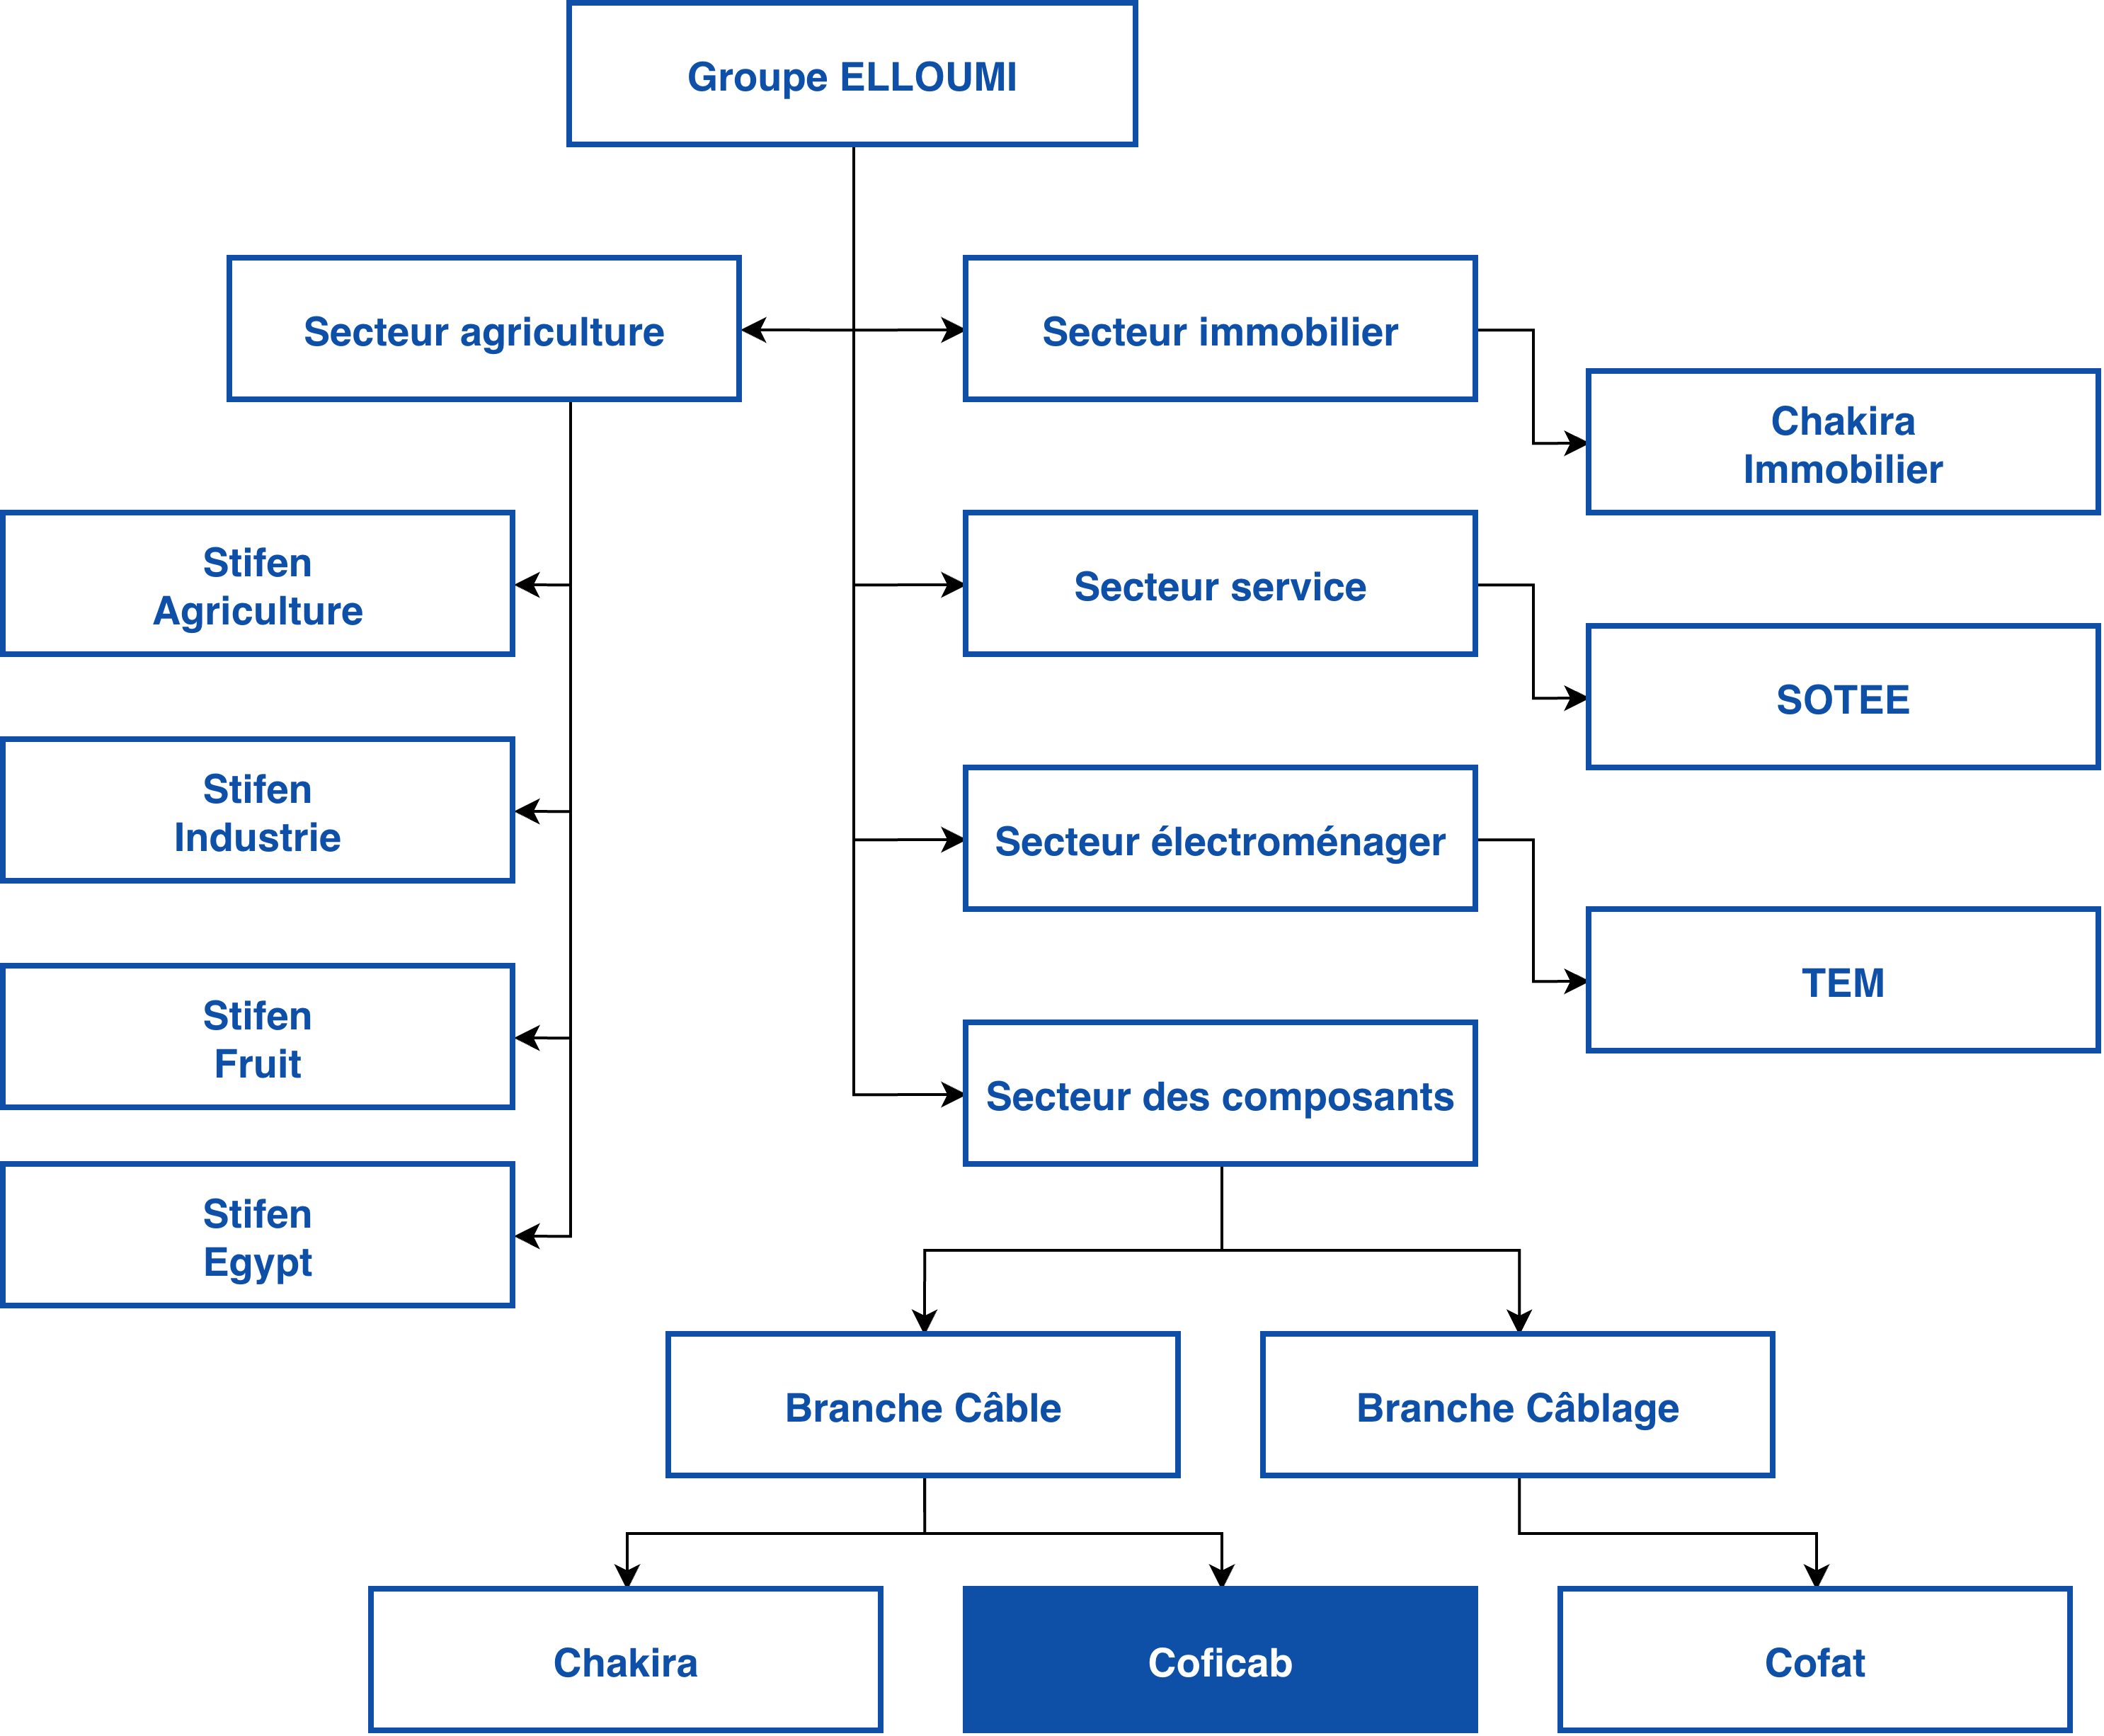
\includegraphics[width=0.78\linewidth]{figures/chapitre-01/groupe_elloumi.png}
  \caption{Organigramme du groupe Elloumi.}
  \label{fig:Organigramme_groupe_Elloumi}
\end{figure}

\subsection{Présentation de l’entreprise COFICAB}
COFICAB \cite{coficab-website} est une entreprise industrielle internationale fondée en 1992 et  spécialisée dans la conception, la fabrication et la commercialisation de câbles et fils électriques pour l’industrie automobile. Elle détient environ 23\% de part de marché mondiale et accompagne les évolutions technologiques du secteur, notamment en mobilité électrique, sécurité et performance. Grâce à une implantation internationale couvrant quatre continents et seize pays, COFICAB opère à travers un réseau structuré de sites industriels, de centres de recherche et d’unités commerciales, employant environ 9 000 collaborateurs.

La figure 1.2 présente le logo de la société COFICAB.
\vspace{0.5cm}
\begin{figure}[H]
  \centering
  
\includegraphics[width=0.4\linewidth]{figures/chapitre-01/coficab-logo.png}
  \caption{Logo de COFICAB.}
  \label{fig:Logo_Coficab}
\end{figure}
Pour mieux comprendre la stratégie de COFICAB, il est essentiel d’analyser l’implantation de ses unités de production, ce qui permet de mettre en évidence sa stratégie territoriale et son positionnement sur les marchés \cite{global-footprint-coficab}.

La figure 1.3 présente la répartition géographique des sites de COFICAB.


\begin{figure}[H]
  \centering
  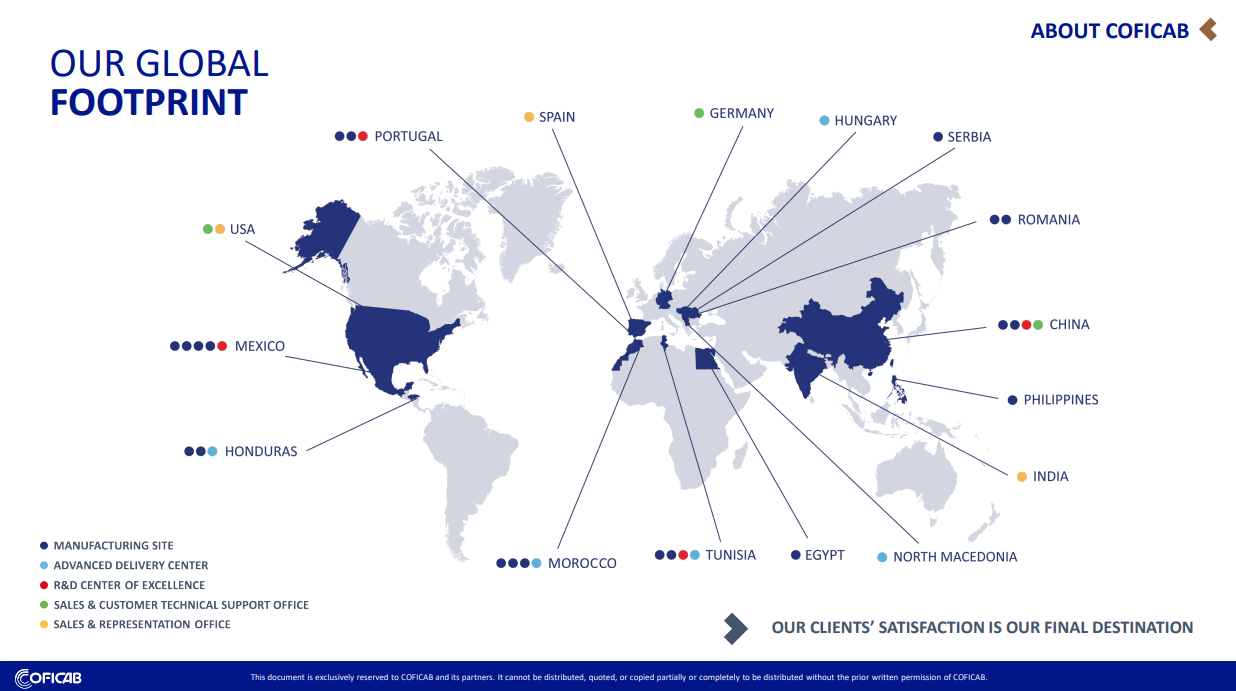
\includegraphics[width=1\linewidth]{figures/chapitre-01/global_footprint_coficab.png}
  \caption{Implantations géographiques de COFICAB.}
  \label{fig:doc-ch1-3}
\end{figure}

\subsection{Outils de gestion utilisés au sein de la société}
Afin d’assurer une gestion efficace et structurée de ses activités, COFICAB s’appuie sur des outils de gestion modernes et intégrés, permettant d’optimiser les processus internes, de faciliter la prise de décision et d’améliorer la performance globale de l’entreprise.
Les principaux outils utilisés sont :

\begin{itemize}[label=\textbullet]
  \item \textbf{Odoo \cite{odoo-docs}} : pour la gestion intégrée des processus de production, logistique, ressources humaines et finance.
  \item \textbf{Power BI \cite{powerbi-docs}} : pour le pilotage de la performance, la création de tableaux de bord et le suivi des KPI\footnote{KPI : \emph{Key Performance Indicator} (indicateur clé de performance). Il s’agit de mesures quantitatives permettant d’évaluer l’atteinte des objectifs et de piloter la performance organisationnelle ou opérationnelle.}.
  \item \textbf{MES\footnote{MES : \emph{Manufacturing Execution System}. Il s’agit d’un système d’exécution de la production permettant de suivre et piloter les opérations de fabrication en temps réel (traçabilité, contrôle, collecte des données de production, indicateurs).} \cite{mes-docs}} : pour le suivi en temps réel des opérations de production, la traçabilité des produits et le contrôle des processus industriels.
  \item \textbf{Trello \cite{trello-docs}} : pour faciliter la communication interne, la gestion documentaire et le travail en équipe.
\end{itemize}
L’utilisation combinée de ces outils contribue à l’amélioration continue des processus, à l’optimisation des performances et au maintien de la compétitivité internationale de COFICAB.

\section{Cadre général du projet}

\subsection{Problématique}

Face aux enjeux croissants liés à la Responsabilité Sociale des Entreprises (RSE) et à la nécessité d’un pilotage performant des actions environnementales, sociales et de gouvernance, les grandes organisations industrielles doivent aujourd’hui disposer de systèmes d’information fiables, centralisés et orientés décision. La multiplication des sites, la diversité des initiatives RSE et l’exigence de reporting structuré rendent les méthodes traditionnelles basées sur des fichiers Excel et des échanges par emails insuffisants pour assurer un suivi efficace et cohérent.

Dans ce contexte, la société COFICAB a exprimé le besoin de mettre en place une solution permettant de planifier, suivre, consolider et analyser les activités RSE à l’échelle de l’ensemble de ses sites.

\subsection{Définition de la mission}

Le présent projet consiste à concevoir et développer une plateforme RSE centralisée, destinée à améliorer la gouvernance, la visibilité et la prise de décision au niveau corporate. La mission principale de ce projet est de :


\begin{itemize}[label=\textbullet, itemsep=0.15ex, parsep=0pt, topsep=0pt, partopsep=0pt]
  \item Concevoir une plateforme web permettant la planification annuelle des activités RSE par site avec un processus de validation structuré.
  \item Assurer le suivi en temps réel des activités réalisées, incluant les activités hors plan.
  \item Centraliser les données RSE afin de fournir une vue consolidée au niveau corporate.
  \item Mettre en place des tableaux de bord Power BI et des indicateurs clés de performance (KPI) Power BI afin d’analyser le taux de réalisation des plans, les budgets des activités, la participation... 
  \item Faciliter l’analyse historique et la gestion des changements à travers un mécanisme de demandes de modification pour les périodes clôturées
\end{itemize}

Cette plateforme vise ainsi à renforcer la performance RSE de COFICAB, à fiabiliser le reporting et à soutenir la prise de décision stratégique grâce à une exploitation optimale des données.

\subsection{Objectifs à atteindre}

Les principaux objectifs que nous visons à atteindre à travers notre application sont :

\begin{enumerate}
  \item \textbf{Centraliser et structurer la gestion des activités des sites dans une plateforme unique}.
  \item \textbf{Fiabiliser le suivi des plans et des activités sur l’ensemble du cycle de vie} avec un workflow de validation, des statuts maîtrisés et une historisation des opérations.
  \item \textbf{Renforcer le contrôle d’accès et la sécurité des données sensibles} par une authentification sécurisée, une gestion des rôles et une restriction d’accès par site.
  \item \textbf{Améliorer la gestion des demandes de modification et la traçabilité des actions} sur les périodes clôturées et les données déjà validées.
  \item \textbf{Assurer une traçabilité complète des opérations via un journal d’audit (log)} pour suivre les créations, modifications, validations, rejets et suppressions.
  \item \textbf{Intégrer un chatbot d’assistance intelligent} pour guider les utilisateurs, répondre aux questions fréquentes et faciliter l’accès rapide aux informations clés de la plateforme.
  \item \textbf{Optimiser le reporting et l’analyse des performances CSR} par la comparaison planifié/réalisé, le calcul automatique des KPI et des tableaux de bord dynamiques.
\end{enumerate}

\section{Étude de l’existant}

\subsection{Analyse de l’existant}

\subsubsection{Description de la gestion des activités RSE au niveau de COFICAB}

La gestion des activités RSE au sein de COFICAB repose sur une organisation fortement décentralisée et peu structurée. Chaque site industriel gérait de manière autonome ses activités RSE, depuis la phase de planification jusqu’au suivi de leur réalisation, sans cadre unifié ni outil centralisé permettant d’harmoniser les pratiques.

Concrètement, les responsables RSE au niveau des différents sites utilisaient principalement des outils bureautiques classiques, notamment des fichiers Excel pour la planification annuelle (\textit{CSR Plan}), la saisie des données réelles des activités (\textit{CSR Report}) et la consolidation globale (\textit{CSR consolidé}) permettant le calcul des KPIs.

\begin{itemize}[label=\textbullet, itemsep=0.15ex, parsep=0pt, topsep=0pt, partopsep=0pt]
  \item Le CSR Plan représente le plan annuel élaboré par le responsable RSE de chaque site, puis soumis à un processus de validation selon le mode de validation défini. Ce plan regroupe les informations essentielles nécessaires au suivi et à la gestion des activités RSE, notamment l’identifiant du plan, le site concerné, l’année de référence, le mode de validation, le budget alloué ainsi que l’effectif total du site.
  Les activités planifiées associées à ce plan sont décrites à travers plusieurs informations, notamment l’identifiant de l’activité, la catégorie, le partenaire externe éventuel, l’intitulé, l’organisation, le type de contrat, la description, la nature de la collaboration, la périodicité, le budget prévu, l’objectif d’impact, l’unité d’impact, la durée de l’impact, le nombre d’employés impliqués, l’année de démarrage, le numéro d’édition et l’organisateur.
  
  La figure~\ref{fig:doc-ch1-csr-plan-workflow} présente le tableau du plan annuel CSR utilisé pour la planification des activités.
  \begin{figure}[H]
  \centering
  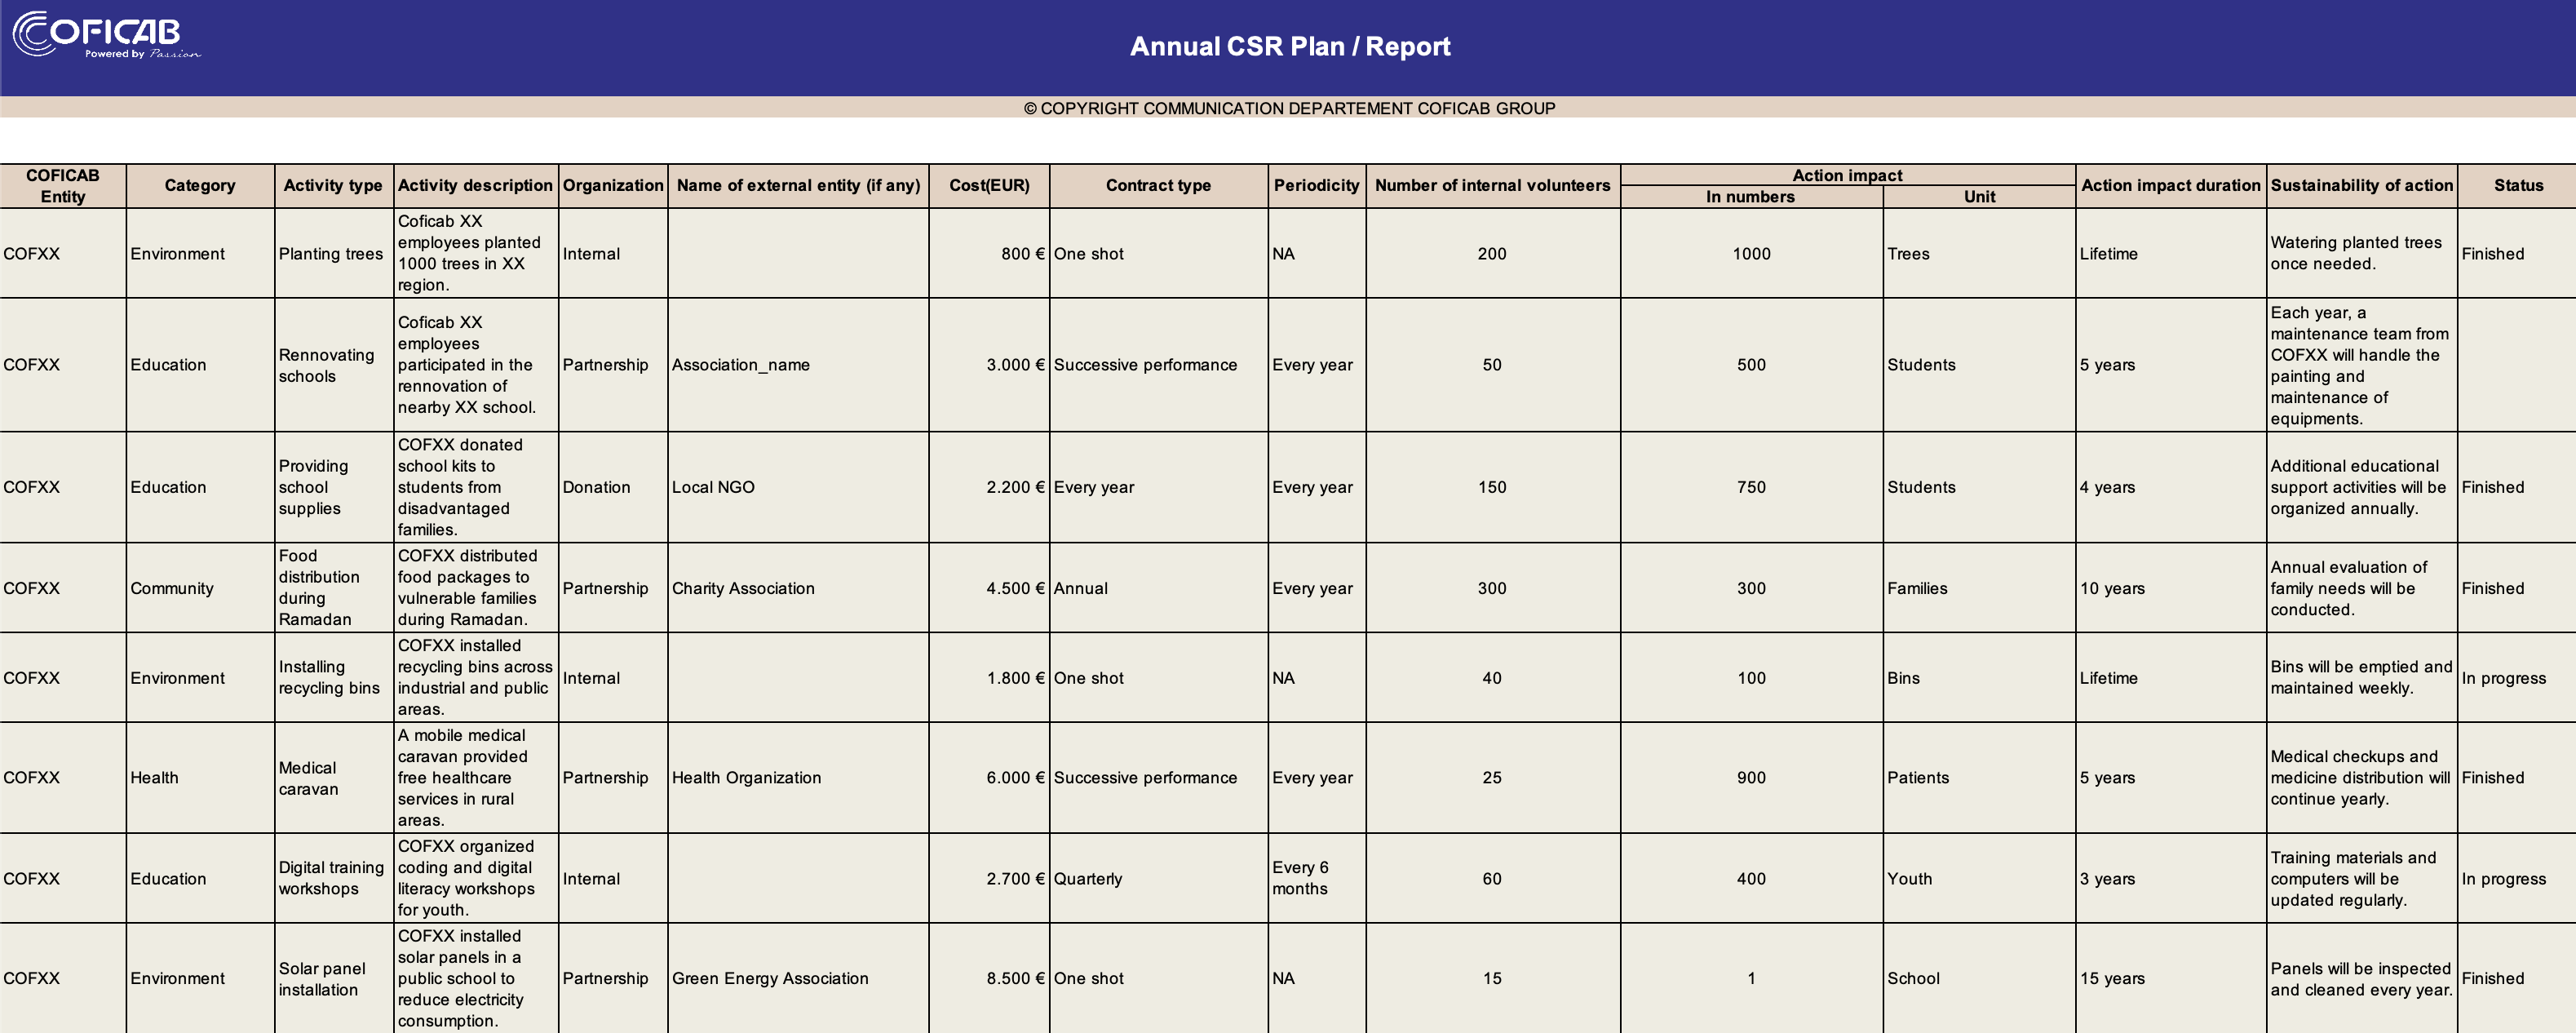
\includegraphics[width=1\linewidth]{figures/chapitre-01/annual-csr-plan.png}
  \caption{Tableau du plan annuel CSR utilisé pour la planification des activités.}
  \label{fig:doc-ch1-csr-plan-workflow}
\end{figure}
\newpage
 \item Le CSR Report correspond aux données réelles des activités réalisées. Il regroupe les informations essentielles liées à chaque activité, telles que l’activité, le nombre de participants, le nombre de participants internes, les indicateurs d’impact, le nombre d’incidents, le département du contact, le budget réellement dépensé, l’impact réalisé, l’unité d’impact, la date de réalisation ainsi que les informations de contact.
 
 La figure~\ref{fig:doc-ch1-csr-report-workflow} présente la formulaire du rapport des activités de contribution sociale.
 \begin{figure}[H]
  \centering
  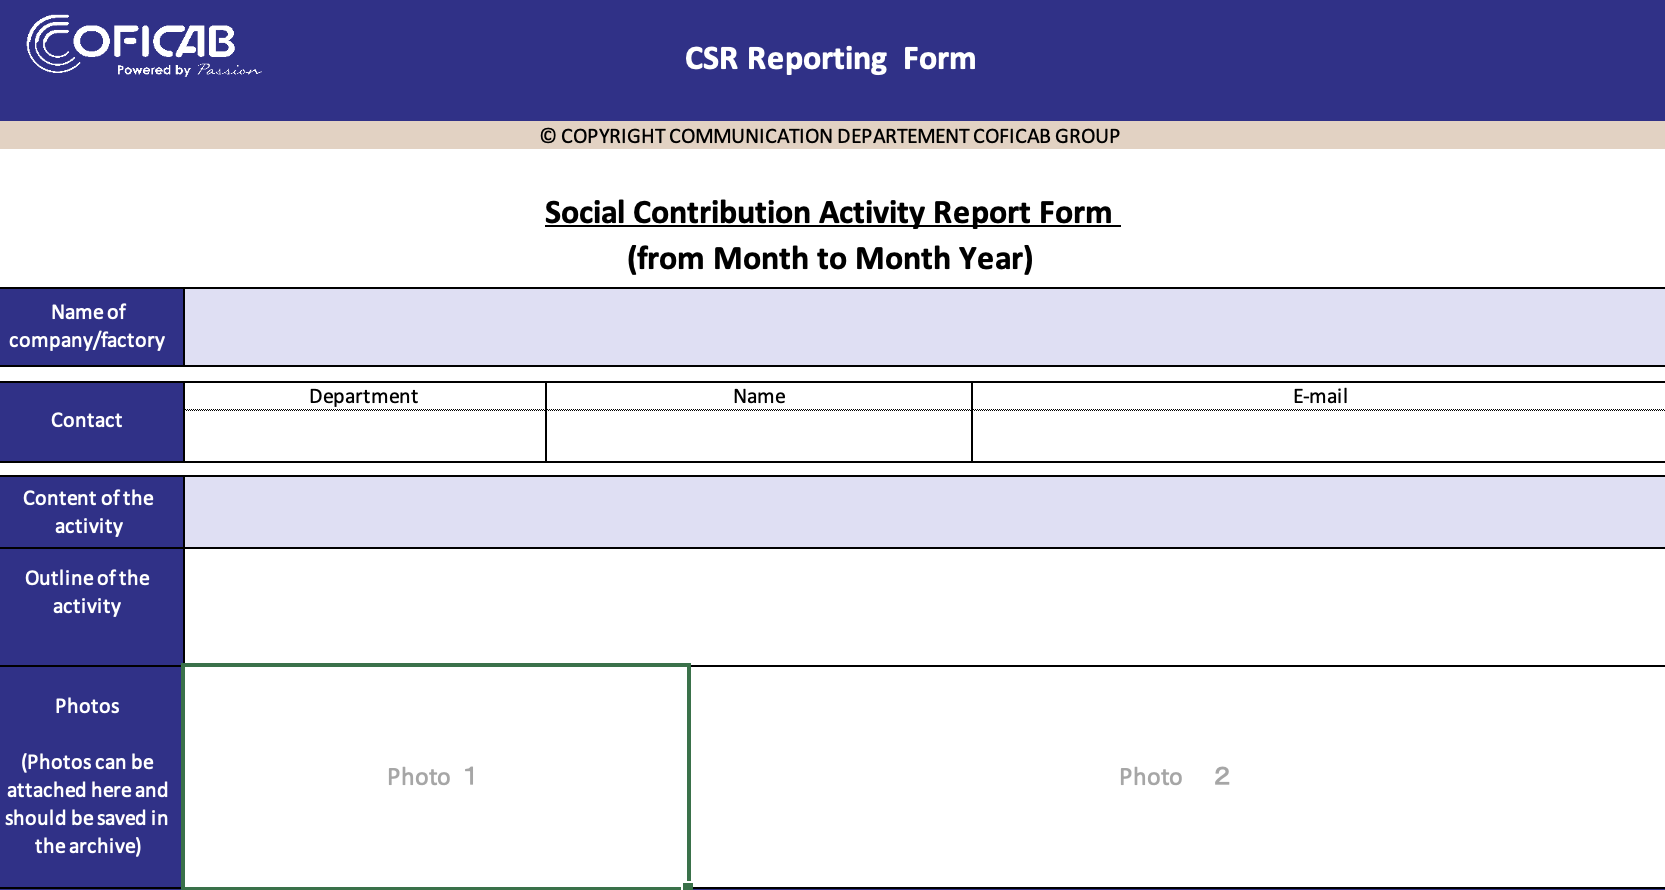
\includegraphics[width=0.9\linewidth]{figures/chapitre-01/csr-report.png}
  \caption{Formulaire du rapport des activités de contribution sociale}
  \label{fig:doc-ch1-csr-report-workflow}
\end{figure}

\item Le CSR Consolidé offre une vue synthétique de l’ensemble des activités RSE réalisées. Il permet de comparer les budgets prévus et réels, d’évaluer les impacts générés et de suivre l’implication des parties prenantes internes et externes. Il constitue un outil de pilotage global facilitant l’analyse et le suivi des performances RSE à l’échelle de l’organisation, en intégrant le calcul des principaux KPI.

La figure~\ref{fig:doc-ch1-csr-kpi-realise} présente le tableau consolidé des activités CSR réalisées.
\begin{figure}[H]
  \centering
  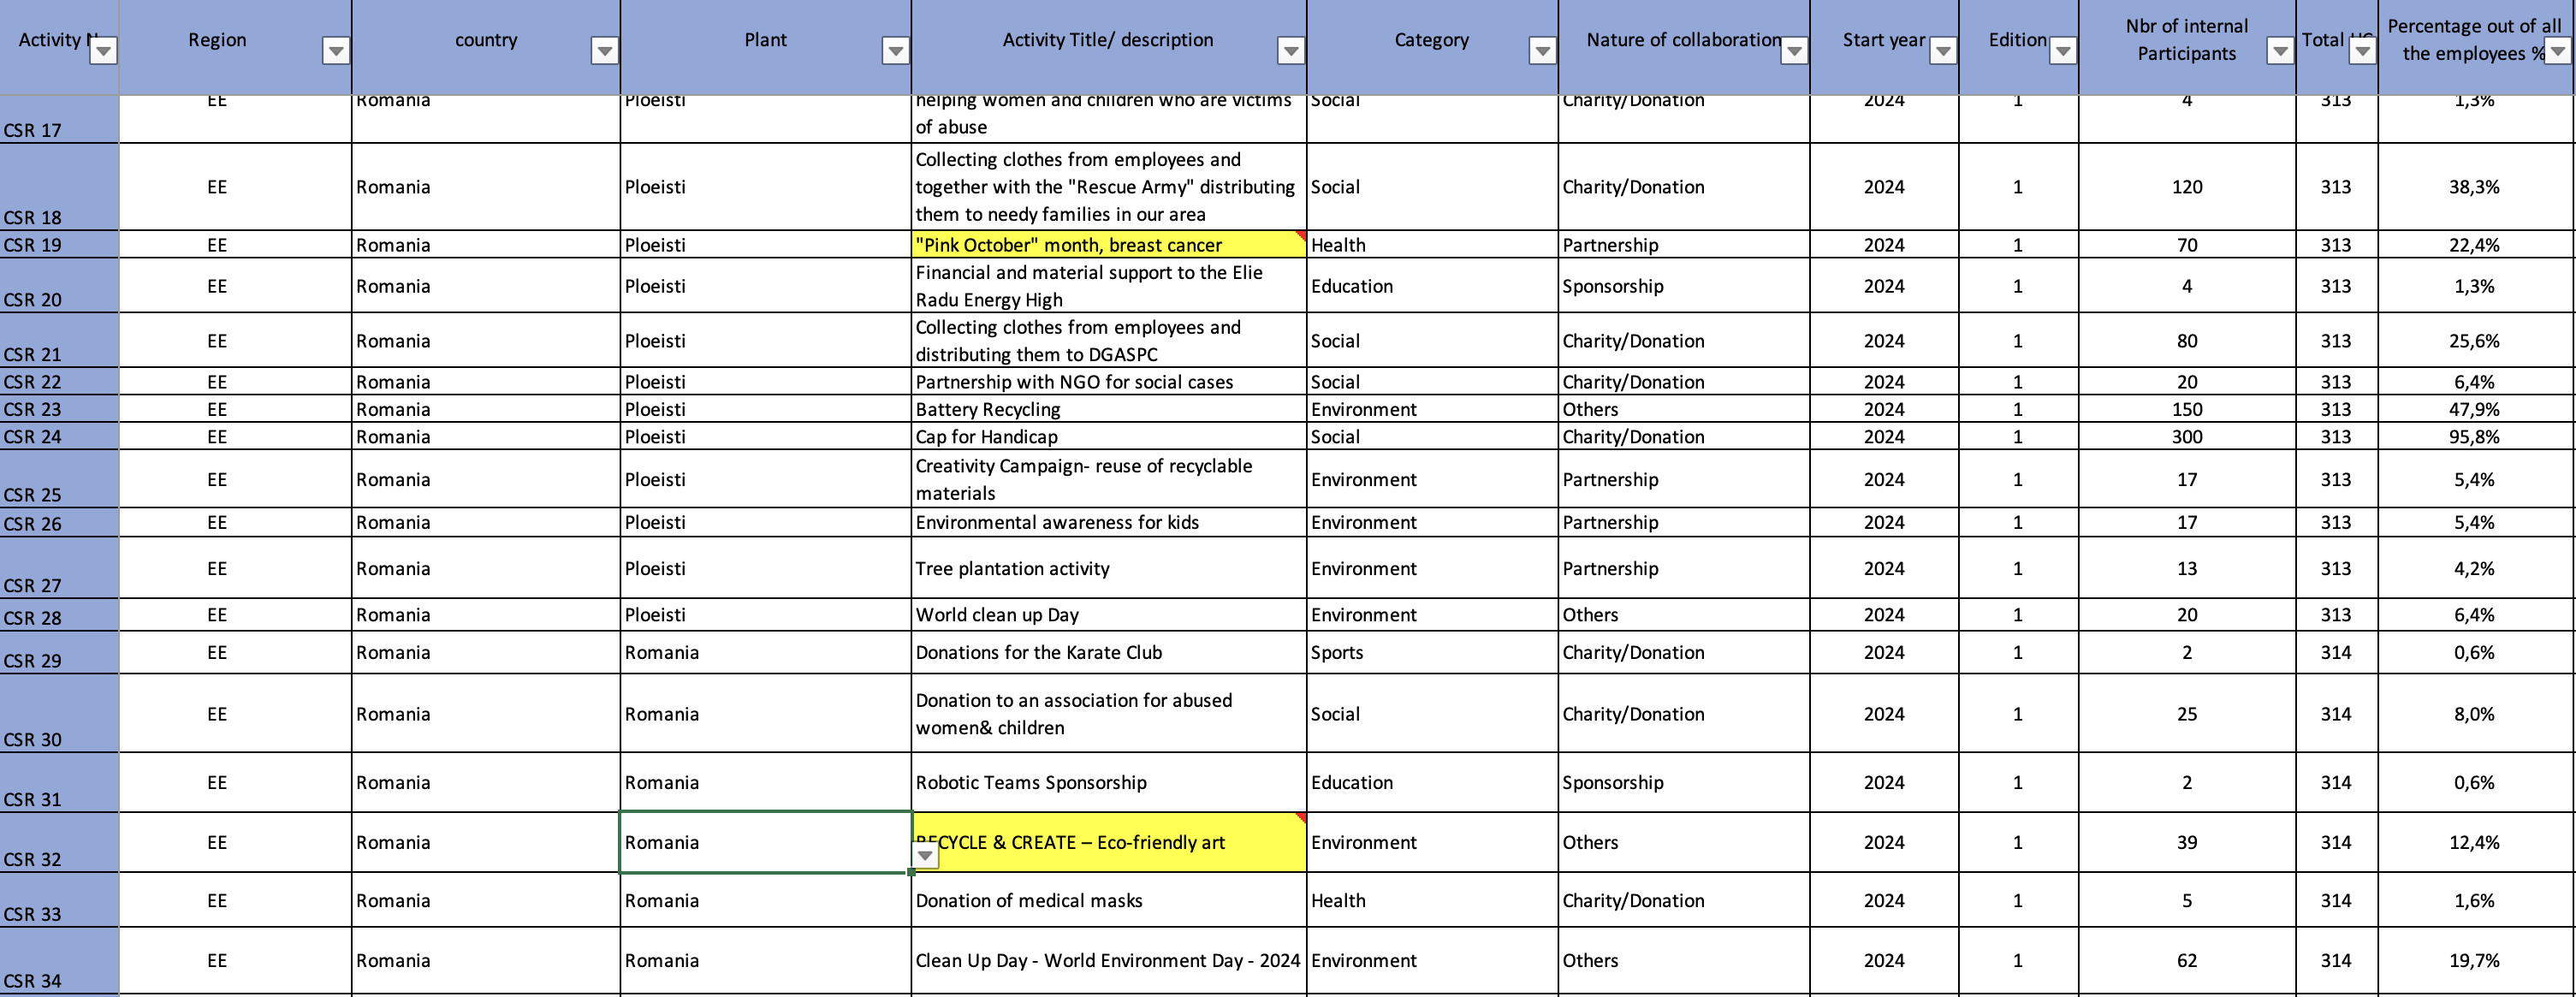
\includegraphics[width=1\linewidth]{figures/chapitre-01/kpi-tout-activitties.png}
  \caption{Tableau consolidé des activités CSR réalisées}
  \label{fig:doc-ch1-csr-kpi-realise}
\end{figure}
\end{itemize}

La figure~\ref{fig:doc-ch1-csr-kpi-workflow} présente un exemple des KPIs calculés à partir du tableau consolidé.
\begin{figure}[H]
  \centering
  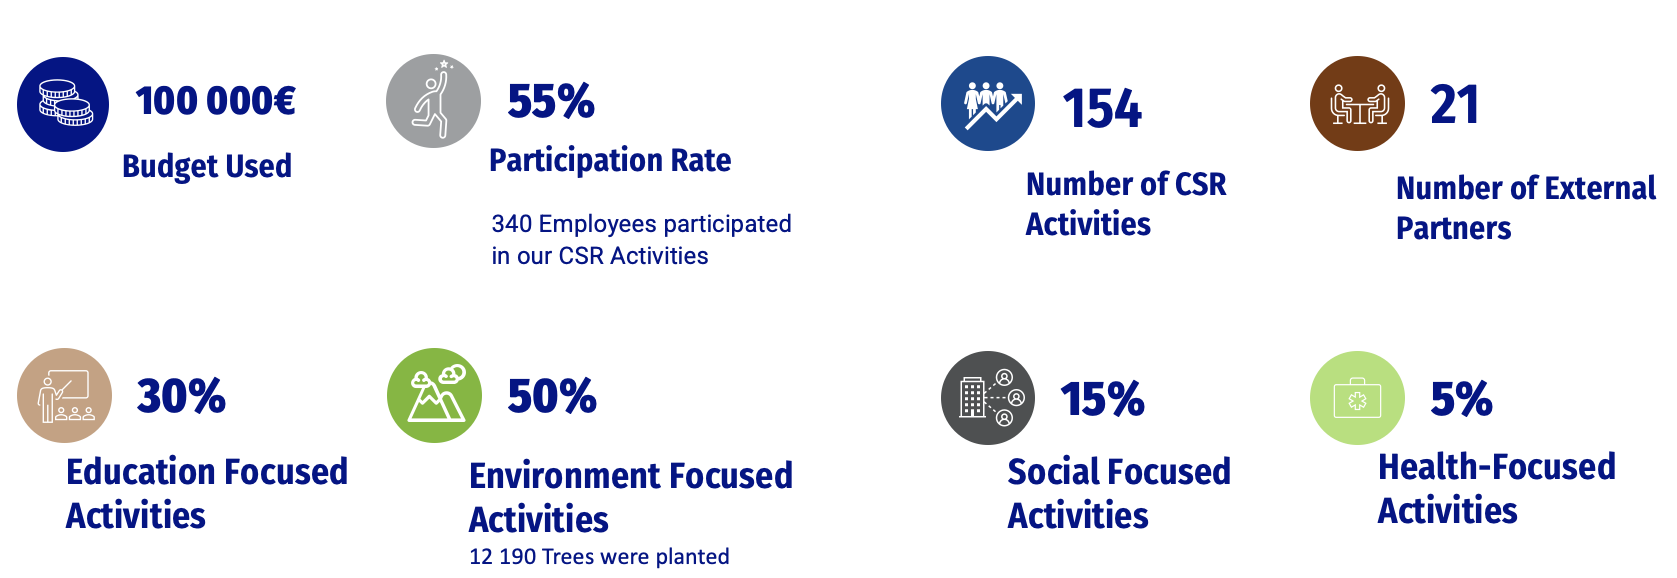
\includegraphics[width=0.9\linewidth]{figures/chapitre-01/exemple-kpi.png}
  \caption{Exemple des KPIs calculés à partir du tableau consolidé.}
  \label{fig:doc-ch1-csr-kpi-workflow}
\end{figure}

Les échanges d’informations se faisaient principalement par email, tandis que chaque site utilisait ses propres formats de fichiers, indicateurs et méthodes de calcul. Les données étaient ensuite regroupées et harmonisées afin de permettre le suivi global des activités RSE et la comparaison entre les différents sites.

Le processus de gestion des activités RSE ne reposait pas sur un workflow de validation formalisé, tandis que le suivi des activités et le reporting étaient réalisés manuellement à partir de plusieurs sources.

La figure~\ref{fig:doc-ch1-workflow-processus-actuel} présente la processus actuel de gestion des activités RSE chez COFICAB.
\begin{figure}[H]
  \centering
  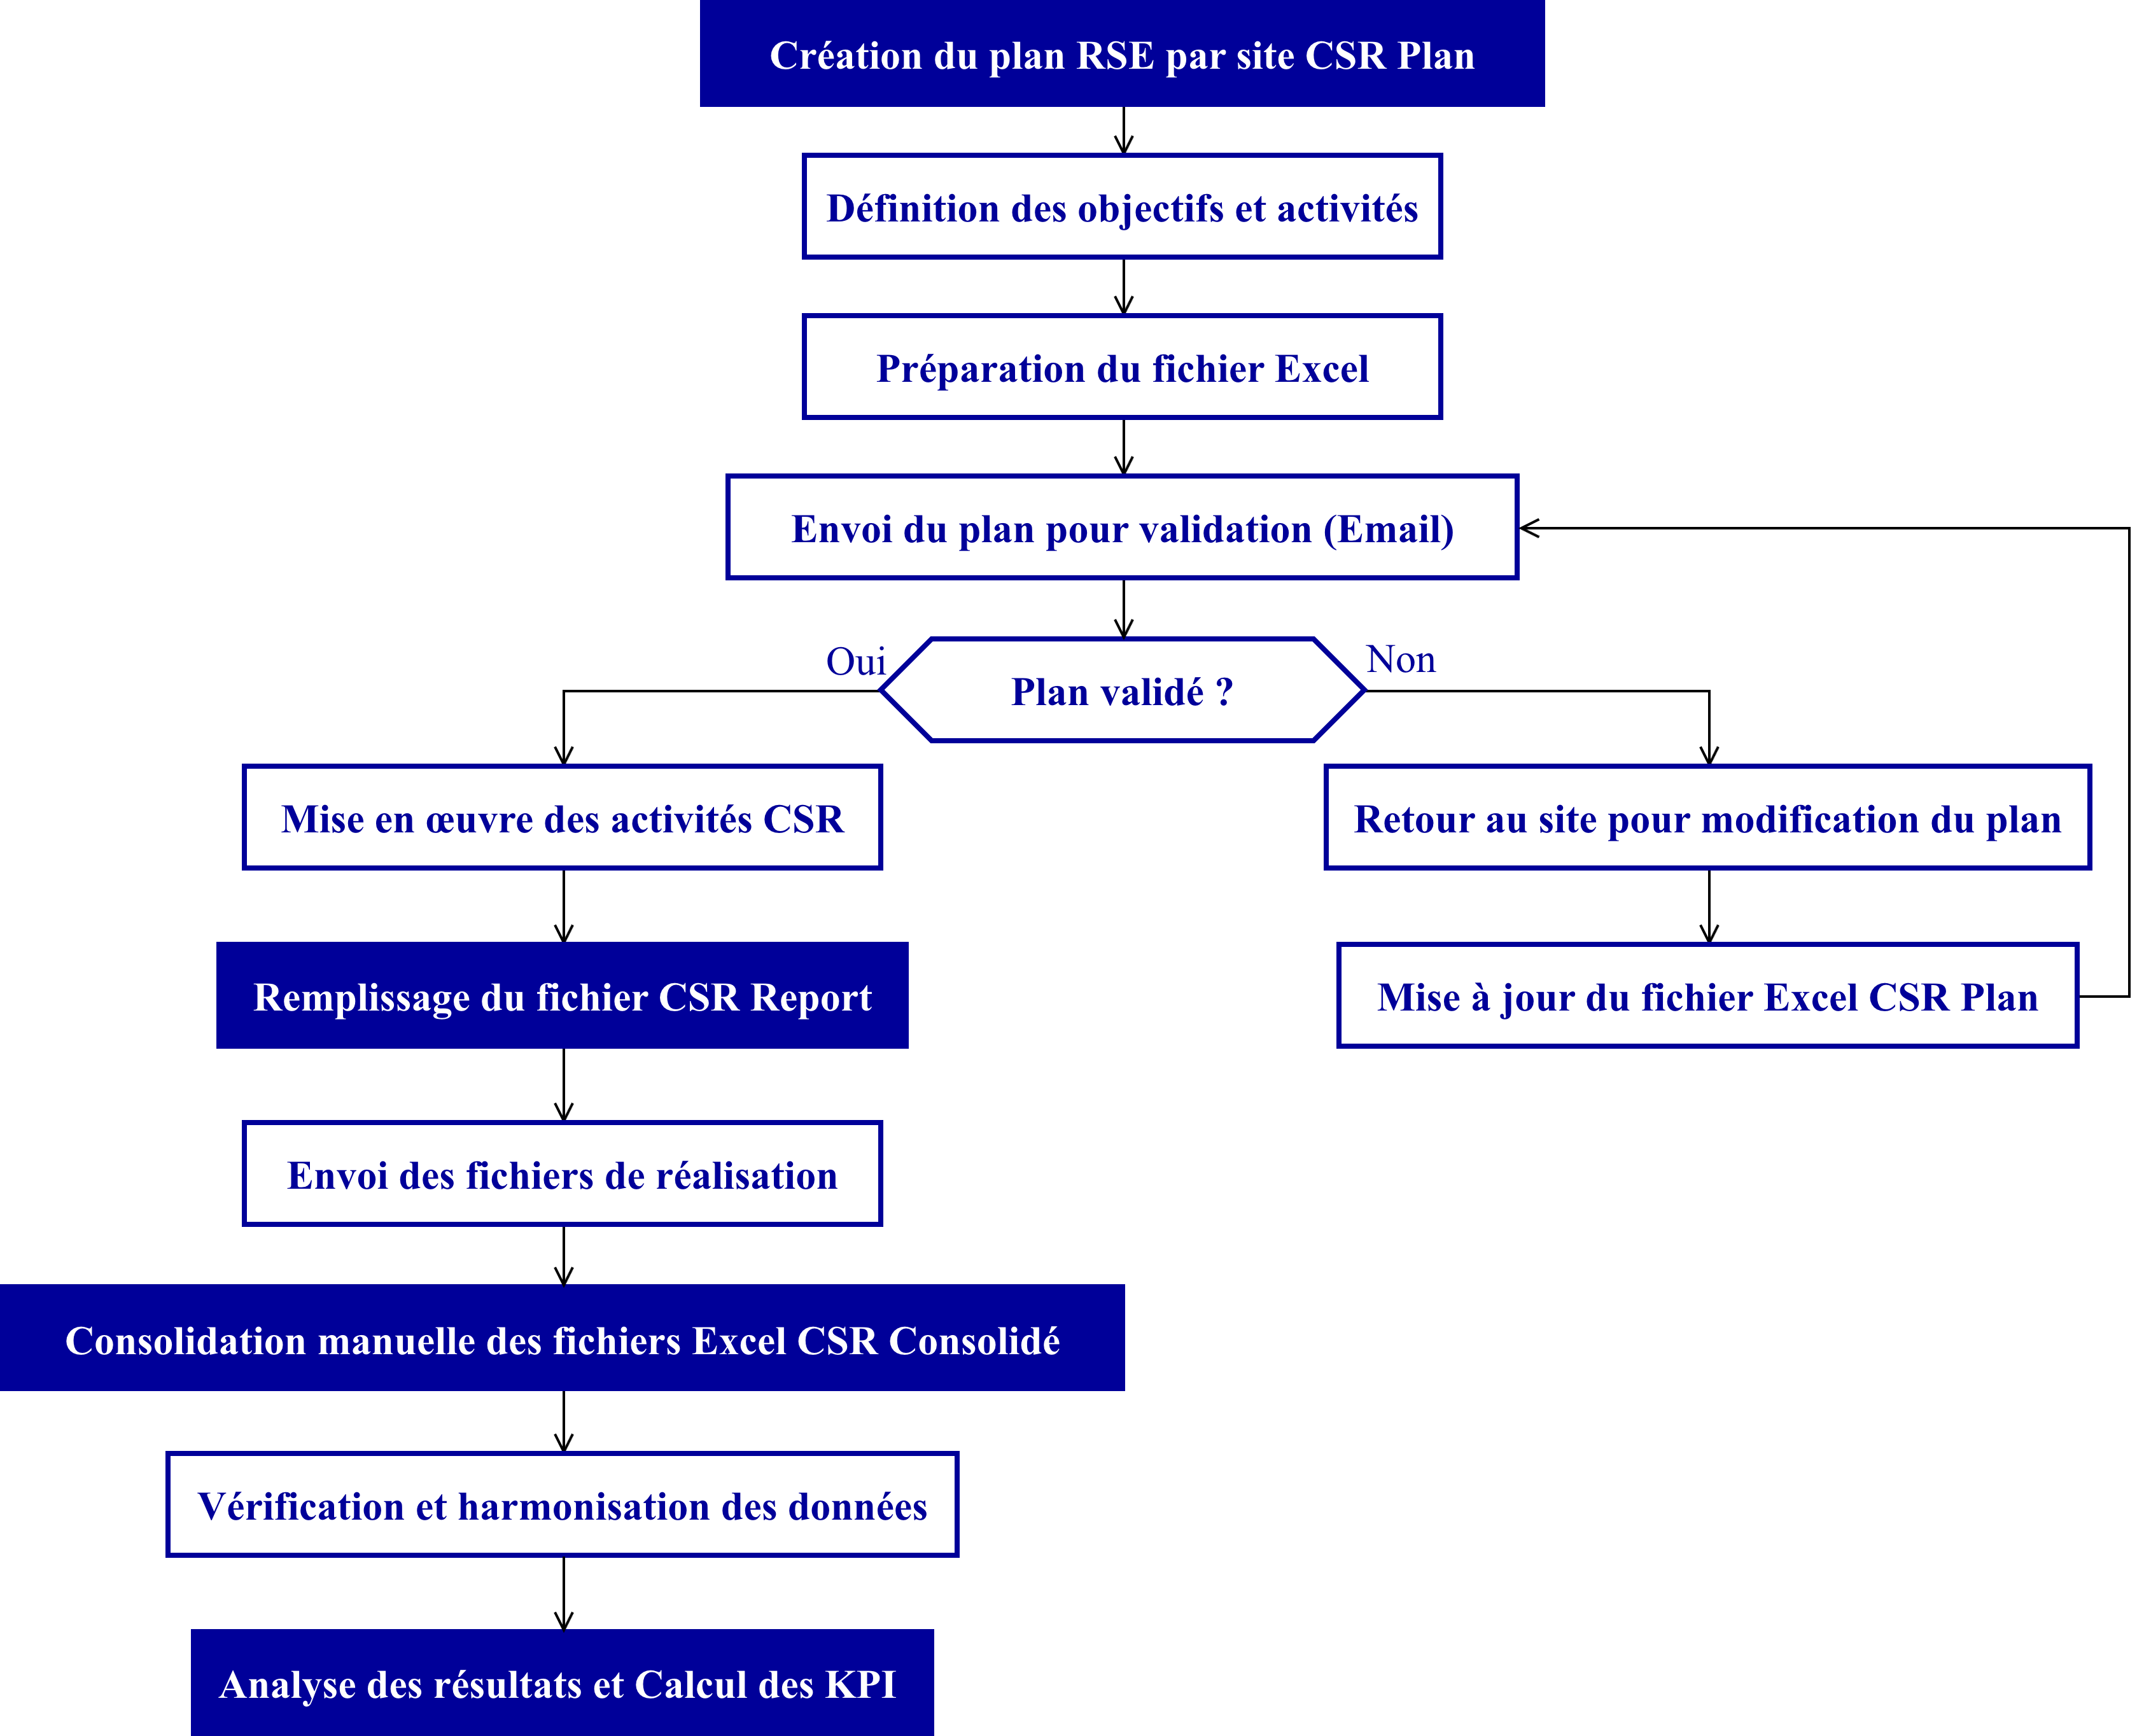
\includegraphics[width=0.85\linewidth]{figures/chapitre-01/workflow_prosessus_actuelle.png}
  \caption{Processus actuel de gestion des activités RSE chez COFICAB.}
  \label{fig:doc-ch1-workflow-processus-actuel}
\end{figure}

\newpage
\subsubsection{Description d’applications d’analyse d’activité RSE similaires}
\begin{itemize}[label=\textbullet]
  \item \textbf{Generous Connect :} \url{www.generousconnect.com}
\end{itemize}


Generous Connect \cite{Generous-Connect} est une plateforme numérique dédiée à la gestion et au suivi des initiatives de responsabilité sociétale des entreprises. Elle permet aux organisations de planifier, coordonner et analyser les activités sociales et environnementales réalisées au sein de leurs sites.

La figure~\ref{fig:doc-ch1-4} présente un aperçu de l’interface de statistiques de Generous Connect.

\begin{figure}[H]
  \centering
  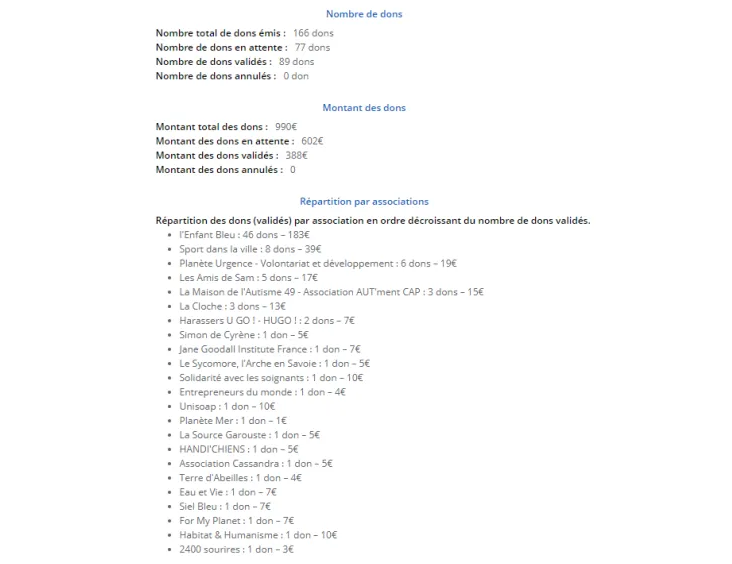
\includegraphics[width=1.1\linewidth]{figures/chapitre-01/generous-connect-statistiques.png}
  \caption{Aperçu de l’interface de statistiques de Generous Connect.}
  \label{fig:doc-ch1-4}
\end{figure}
L’application centralise les informations relatives aux projets RSE, telles que les actions menées, les ressources mobilisées et les indicateurs de performance. Grâce à des outils d’analyse et de reporting, les responsables peuvent suivre l’avancement des initiatives, évaluer leur impact et améliorer la gestion des programmes RSE à travers des tableaux de bord analytiques facilitant la prise de décision.

\newpage
\begin{itemize}[label=\textbullet]
  \item \textbf{Optimy : Solution d’efficacité en gestion de programmes :} \url{www.optimy.com}
\end{itemize}
Optimy \cite{Optimy} est une plateforme spécialisée dans la gestion et le suivi des programmes d’impact, notamment les initiatives de responsabilité sociétale des entreprises. Elle permet aux entreprises de planifier, organiser et gérer efficacement leurs projets sociaux, environnementaux ou de sponsoring.

La solution centralise les informations liées aux programmes, facilite le suivi des activités et permet de mesurer leur performance à l’aide d’indicateurs et de rapports analytiques. Grâce à ses outils de gestion et de reporting, Optimy aide les responsables à évaluer l’impact des initiatives et à améliorer la prise de décision dans la gestion des programmes RSE.

La figure~\ref{fig:doc-ch1-5} présente un aperçu du tableau de bord de la plateforme Optimy.

\begin{figure}[H]
  \centering
  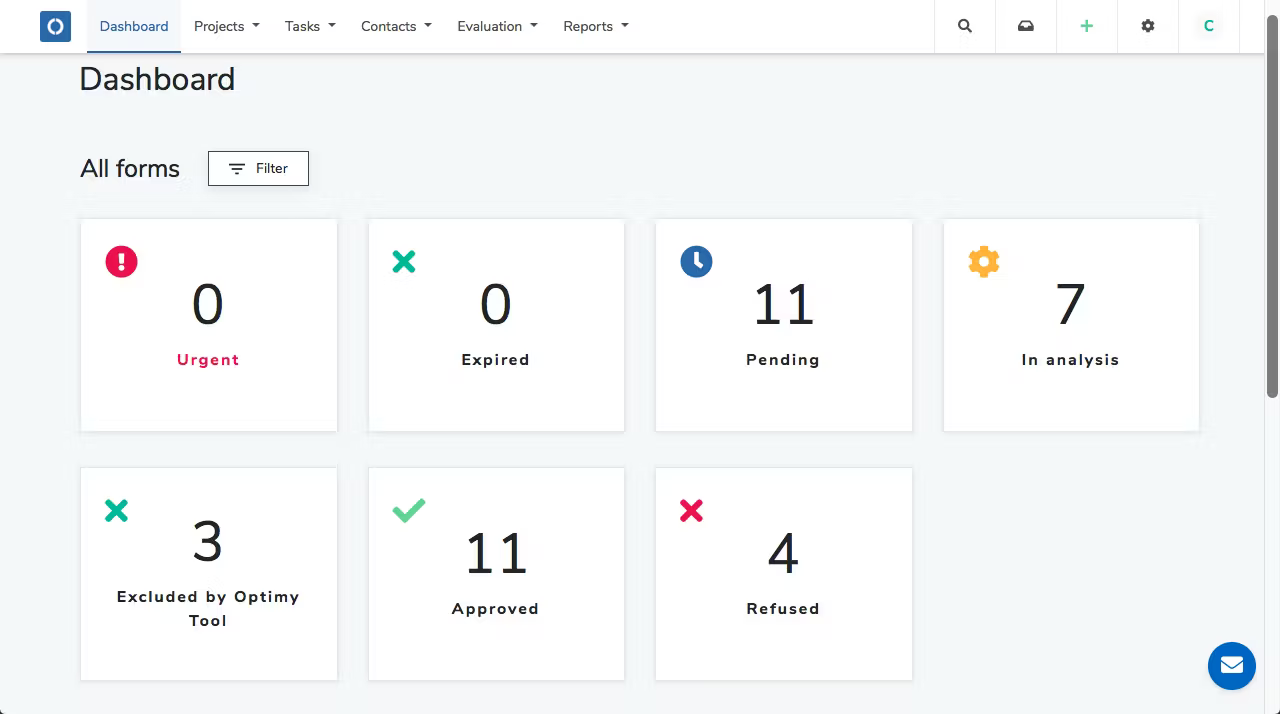
\includegraphics[width=1.1\linewidth]{figures/chapitre-01/optimy-dashboard.png}
  \caption{Aperçu du tableau de bord de la plateforme Optimy.}
  \label{fig:doc-ch1-5}
\end{figure}
\newpage
\subsection{Critique de l’existant}

\subsubsection{Critique des activités RSE au niveau de COFICAB}

L’analyse du système actuel de gestion des activités RSE au sein de COFICAB révèle plusieurs limites. 
\begin{itemize}[label=\textbullet, itemsep=0.15ex, parsep=0pt, topsep=0pt, partopsep=0pt]
  \item L’utilisation de fichiers Excel et de documents dispersés entraîne une gestion décentralisée et une hétérogénéité des données entre les différents sites. Cette situation rend difficile la consolidation des informations et limite la visibilité globale au niveau corporate.
  \item Le processus de validation des plans reste peu structuré (étapes, statuts, responsabilités), ce qui complique le suivi des approbations, allonge les délais de traitement et réduit la traçabilité des décisions.
  \item La comparaison entre les données planifiées et les données réelles n’est pas réalisée de manière systématique ni fiable, ce qui limite l’identification rapide des écarts de budget, d’impact et d’avancement des activités.
  \item Le reporting repose sur un traitement manuel des données, ce qui est chronophage et augmente le risque d’erreurs.
  \item L’absence d’un système centralisé et d’outils d’analyse adaptés réduit également la capacité de l’entreprise à suivre efficacement ses performances RSE et à prendre des décisions basées sur des indicateurs fiables.
\end{itemize}
Dans ce contexte, le système existant de gestion des activités RSE ne permettait ni un suivi efficace et structuré des activités RSE par site, ni une vision consolidée au niveau corporate, ni une analyse approfondie basée sur des KPI pertinents. Ces limitations ont mis en évidence la nécessité de concevoir et de déployer une plateforme CSR intégrée, capable de centraliser les données, standardiser les processus, automatiser les workflows de validation et offrir des outils avancés d’analyse et de reporting.
\subsubsection{Critique des applications similaires}

Les plateformes telles que Generous Connect et Optimy offrent des solutions avancées pour la gestion des programmes RSE. Cependant, ces solutions restent généralement génériques et ne répondent pas toujours aux besoins spécifiques de chaque entreprise.

De plus, leur adoption peut impliquer des coûts importants liés aux licences et à l’intégration. Leur niveau de personnalisation peut également être limité, ce qui rend parfois difficile leur adaptation complète aux processus internes de l’organisation.

Le tableau~\ref{tab:analyse-comparative-rse} présente une analyse comparative entre les différentes solutions existantes et les processus actuels de COFICAB.

\begin{table}[H]
  \centering
  \small
  \caption{Analyse comparative entre le processus actuel COFICAB et les solutions RSE}
  \label{tab:analyse-comparative-rse}
  \PFETableSetup
  \PFETableRowColors
  \PFETableArrayStretch
  \PFETableTabularXBegin
  \begin{tabularx}{\PFETableBlockWidth}{@{}%
    >{\raggedright\arraybackslash\hsize=1.40\hsize}X%
    >{\centering\arraybackslash\hsize=0.775\hsize}X%
    >{\centering\arraybackslash\hsize=0.775\hsize}X%
    >{\centering\arraybackslash\hsize=0.775\hsize}X%
  @{}}
    \tableHeaderStyle \tableHeaderCell{Critères} & \tableHeaderCell{Processus actuel COFICAB} & \tableHeaderCell{Generous Connect} & \tableHeaderCell{Optimy} \\
    Centralisation des données & absent & limité & présent \\
    Visibilité globale des activités & absent & présent & présent \\
    Suivi des activités RSE & partiellement & présent & présent \\
    Validation des plans et activités & absent & partiellement & absent \\
    Comparaison planifié et réalisé & absent & limité & absent \\
    Reporting et tableaux de bord & absent & limité & présent \\
    Analyse des indicateurs (KPI) & absent & partiellement & présent \\
    Personnalisation selon les besoins de l’entreprise & présent & limité & limité \\
  \end{tabularx}%
  \PFETableTabularXEnd
\end{table}


\section{Solution proposée}

En tenant compte des limites des systèmes existants et des objectifs fixés, nous proposons de développer une plateforme web centralisée de gestion de la Responsabilité Sociétale des Entreprises (RSE), conçue pour aider les différentes entités de COFICAB à planifier, suivre et évaluer leurs activités CSR à l’échelle de tous leurs sites.

\begin{itemize}[label=\textbullet, itemsep=0.15ex, parsep=0pt, topsep=0pt, partopsep=0pt]
  \item La plateforme permettra à chaque site de définir son plan annuel,  en précisant : les activités à réaliser, les catégories (Environnement, Social. . .), les budgets prévisionnels, les périodes de réalisation, les responsables et les indicateurs de performance. Ces plans passent par un workflow de validation structuré, assurant l’alignement avec la stratégie globale.
  \item Tout au long de l’année, la plateforme permettra aux sites de saisir en temps réel les activités réalisées, incluant coûts, nombre de participants, impact et documents justificatifs (rapports, photos). Ainsi, la plateforme permettra un suivi continu et une comparaison automatique entre activités planifiées et réalisées.
  \item La sécurité sera assurée à travers une authentification sécurisée, une gestion des rôles et permissions (site/corporate), un contrôle d’accès par site et une traçabilité complète des opérations via un journal d’audit.
  \item Un entrepôt de données sera construit pour consolider les données historiques et préparer les analyses décisionnelles. Le processus ETL sera implémenté avec SSIS pour extraire, transformer, nettoyer et charger les données issues du système opérationnel.
  \item Au niveau corporate, la plateforme fournira un tableau de bord consolidé donnant une vision globale de la performance. Les décideurs peuvent analyser des indicateurs tels que le taux de réalisation, les écarts budgétaires, la participation et l’évolution de l’impact, grâce à des visualisations interactives et des rapports détaillés.
  \item En remplaçant les outils manuels comme Excel et les échanges par e-mail, la solution améliore la visibilité, cohérence et traçabilité, renforce la collaboration entre sites et direction, facilite la prise de décision basée sur les données et permet d’évaluer plus efficacement l’impact réel.
\end{itemize}
\section{Méthodologies de gestion de projet}

Dans cette section, nous présentons une étude comparative des différentes méthodologies de gestion de projet et de développement des systèmes d’information afin d’identifier l’approche la plus appropriée pour la réalisation de la plateforme.


\subsection{Revue des méthodologies agiles}

La méthodologie Agile est une approche de gestion de projet qui repose sur l’adaptabilité, la collaboration avec les parties prenantes et la livraison continue de fonctionnalités à forte valeur ajoutée. Elle favorise le découpage du projet en itérations courtes et incrémentales, permettant de réagir rapidement aux changements et d’intégrer les retours des utilisateurs tout au long du cycle de développement.

Cette approche est particulièrement adaptée aux projets informatiques modernes, notamment les applications web, où les besoins évoluent fréquemment. Parmi les frameworks Agile existants nous distinguons Scrum, Kanban, RUP et GIMSI.

\subsubsection{Scrum}

Scrum est un framework Agile basé sur des cycles courts appelés Sprints, généralement de deux à quatre semaines, favorisant la transparence, le suivi continu et l’amélioration progressive. Le projet débute par la définition des besoins, gérés dans un Product Backlog par le Product Owner sous forme de User Stories. Chaque Sprint commence par une planification, suivie de réunions quotidiennes pour suivre l’avancement et résoudre les obstacles. Il se termine par une revue des livrables et une rétrospective pour améliorer le processus \cite{pm-partners-scrum-overview}.




La figure~\ref{fig:doc-ch1-7} présente une vue d’ensemble du processus Scrum.

\begin{figure}[H]
  \centering
  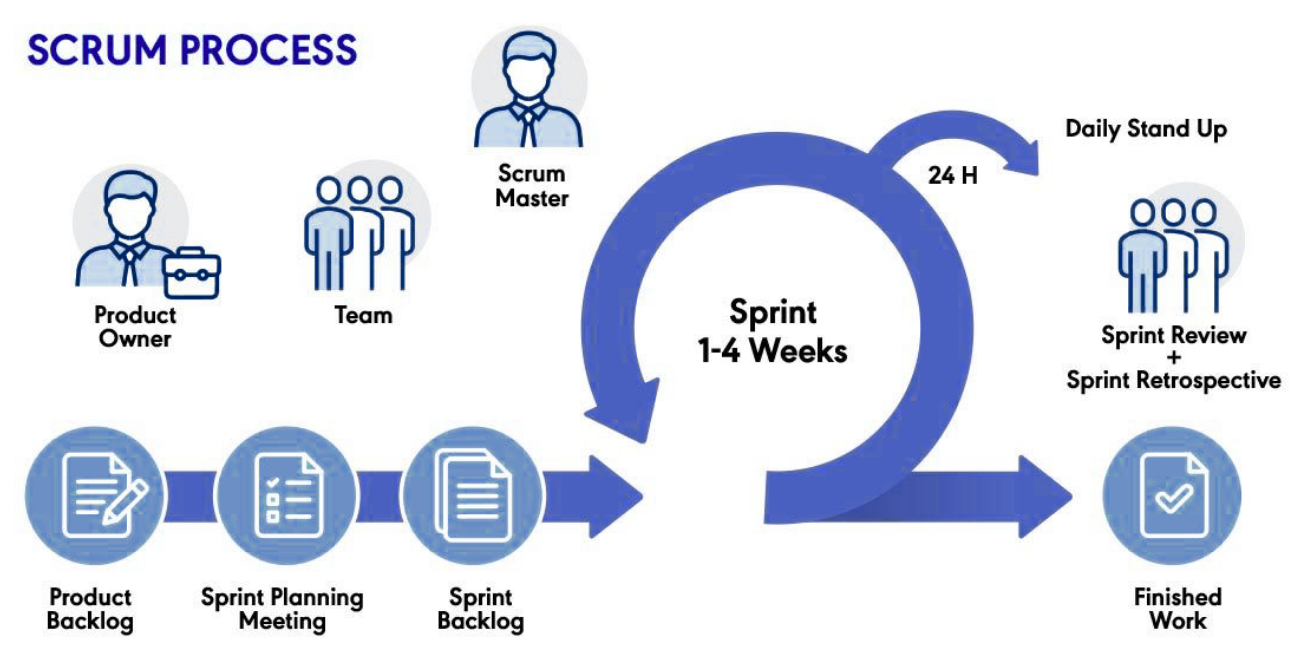
\includegraphics[width=0.8\linewidth]{figures/chapitre-01/scrum-process.png}
  \caption{Vue d’ensemble du processus Scrum.}
  \label{fig:doc-ch1-7}
\end{figure}

\subsubsection{Kanban}

Kanban est une méthode Agile orientée flux continu, basée sur la visualisation des tâches et la limitation du travail en cours. Les activités sont organisées dans un tableau composé de colonnes représentant les étapes du processus. Cette approche permet d’identifier rapidement les blocages, de fluidifier l’avancement et d’améliorer les délais de traitement \cite{kanban-method}.

La figure~\ref{fig:doc-ch1-8} présente une vue d’ensemble du processus Kanban.

\begin{figure}[H]
  \centering
  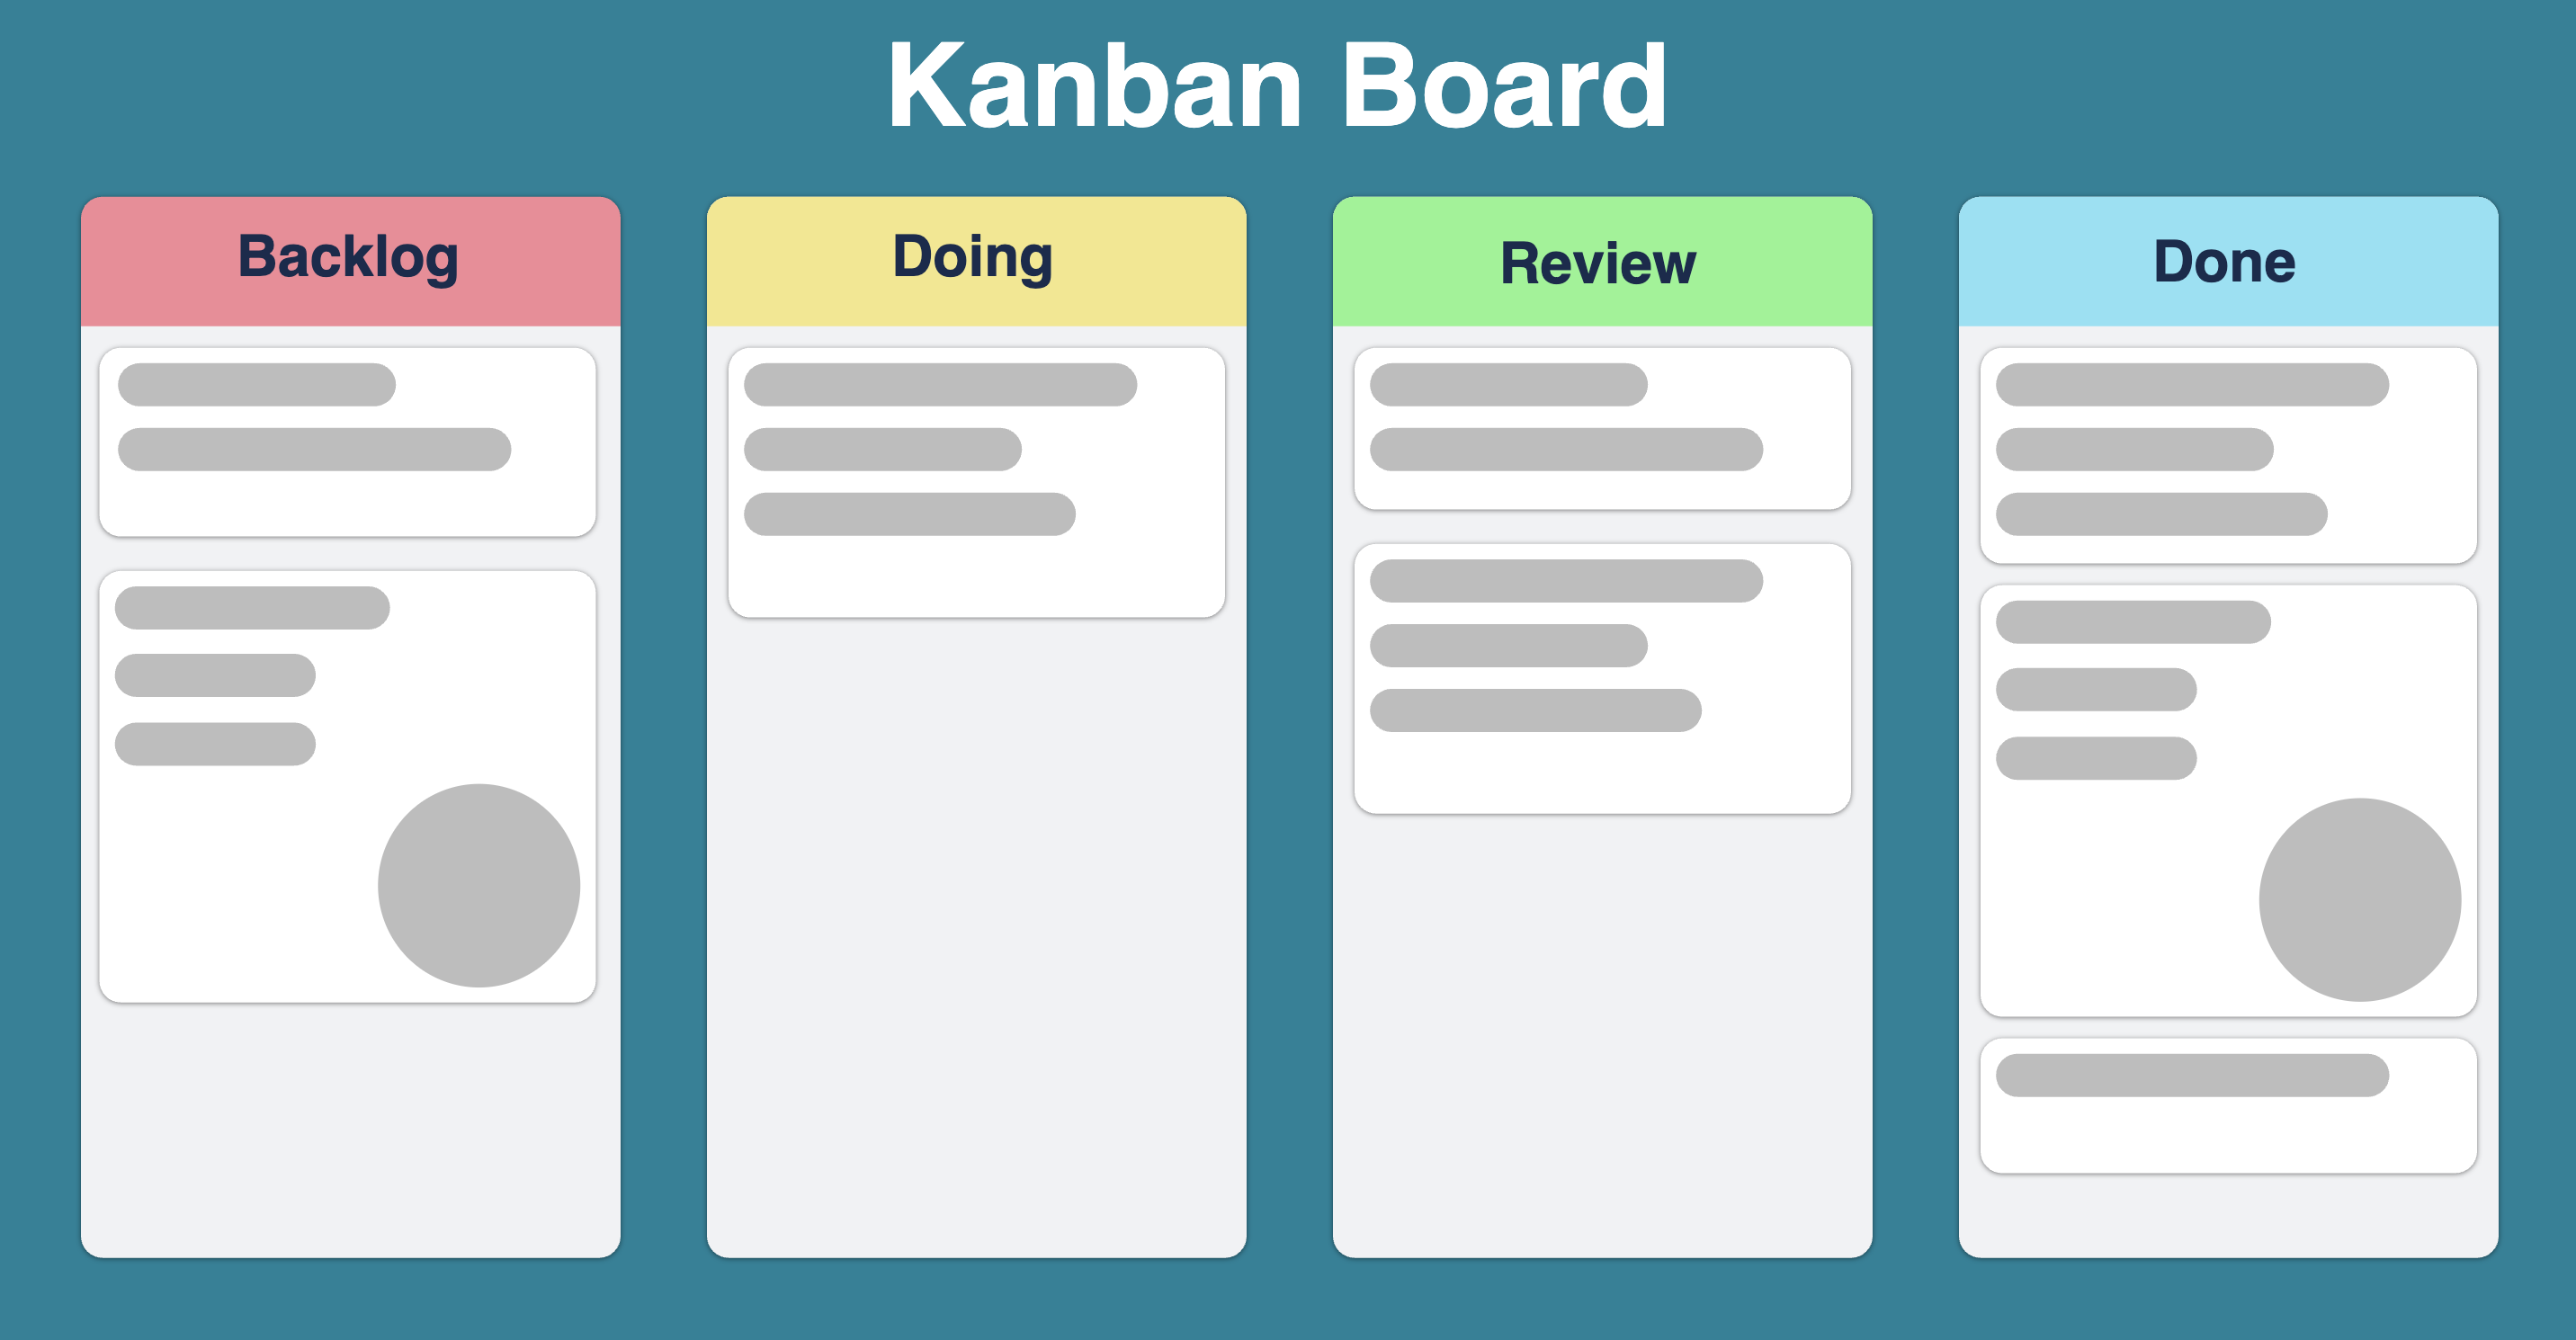
\includegraphics[width=0.7\linewidth]{figures/chapitre-01/kanban-process.png}
  \caption{Vue d’ensemble du processus Kanban.}
  \label{fig:doc-ch1-8}
\end{figure}
\subsubsection{Rational Unified Process (RUP)}

RUP est une méthodologie itérative et structurée basée sur quatre phases principales : inception, élaboration, construction et transition. Elle met l’accent sur la modélisation UML, la gestion des risques et une documentation détaillée \cite{sketchbubble-rup}.

Bien que RUP offre une bonne structuration du projet, sa complexité et sa lourdeur documentaire peuvent constituer un frein dans le cadre d’un projet académique à durée limitée.

La figure~\ref{fig:doc-ch1-9} illustre les phases principales de la méthodologie RUP.

\begin{figure}[H]
  \centering
  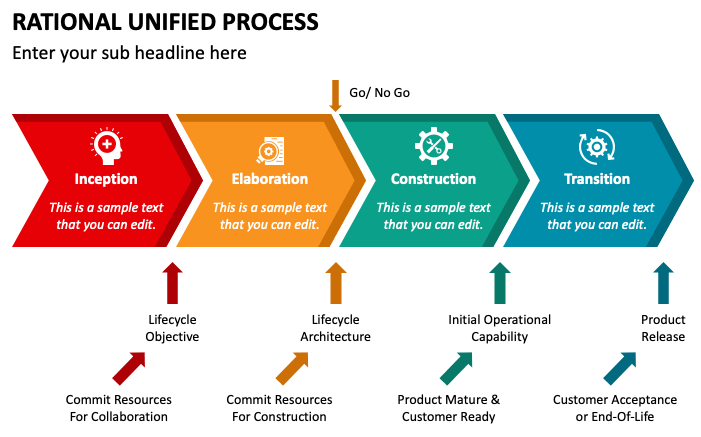
\includegraphics[width=0.92\linewidth]{figures/chapitre-01/rup-phases.png}
  \caption{Phases principales de la méthodologie RUP.}
  \label{fig:doc-ch1-9}
\end{figure}

\subsubsection{GIMSI}

GIMSI est une méthodologie de gestion de projets de systèmes d’information, souvent utilisée pour les projets de Business Intelligence et de tableaux de bord décisionnels. Elle vise à aligner les objectifs métier avec les indicateurs de performance \cite{headmind-bi-intro}.

Cette méthodologie est pertinente pour la partie reporting et indicateurs de performance, mais elle ne couvre pas de manière complète l’ensemble du cycle de développement logiciel.

La figure~\ref{fig:doc-ch1-10} présente les étapes principales de la méthodologie GIMSI.

\begin{figure}[H]
  \centering
  
\includegraphics[width=0.92\linewidth]{figures/chapitre-01/gimsi-etapes-simplifiees.png}
  \caption{Étapes principales de la méthodologie GIMSI.}
  \label{fig:doc-ch1-10}
\end{figure}


\subsection{Comparaison des méthodologies}

Afin de sélectionner la méthodologie la plus adaptée au projet de Plateforme, plusieurs critères ont été définis en tenant compte des spécificités du projet, notamment la gestion multi-sites, l’évolution continue des besoins métier et l’intégration d’une forte composante Business Intelligence.

Les critères d’évaluation retenus sont les suivants :

\begin{itemize}[label=\textbullet, itemsep=0.15ex, parsep=0pt, topsep=0pt, partopsep=0pt]
  \item Orientation du méthodologie
  \item Structure et flexibilité
  \item Couverture du cycle SI
  \item Collaboration \& parties prenantes
  \item Scalabilité \& maintenabilité
  \item Adaptation au projet CSR
  \item Adaptation au BI \& décisionnel
\end{itemize}


\Needspace{22\baselineskip}%
Le tableau~\ref{tab:comparaison-methodes} présente une analyse comparative des méthodologies agiles étudiées.

\begin{table}[H]
  \centering
  \small
  \caption{Analyse comparative des méthodologies agiles étudiées}
  \label{tab:comparaison-methodes}
  \PFETableSetup
  \PFETableRowColors
  \PFETableArrayStretch
  \PFETableTabularXBegin
  \begin{tabularx}{\PFETableBlockWidth}{@{}%
    >{\raggedright\arraybackslash\hsize=0.95\hsize}X%
    >{\raggedright\arraybackslash\hsize=0.95\hsize}X%
    >{\raggedright\arraybackslash\hsize=0.95\hsize}X%
    >{\raggedright\arraybackslash\hsize=0.95\hsize}X%
    >{\raggedright\arraybackslash\hsize=0.95\hsize}X%
  @{}}
    \tableHeaderStyle \tableHeaderCell{Critères} &
    \tableHeaderCell{Scrum} &
    \tableHeaderCell{Kanban} &
    \tableHeaderCell{RUP} &
    \tableHeaderCell{GIMSI} \\

    Nombre d’étapes &
    5 étapes &
    Processus continu &
    4 étapes &
    4 étapes \\

    Étapes principales &
    Initialisation, Planification, Conception, Implémentation, Revue &
    Visualisation du flux, Limitation du travail en cours, Gestion continue du flux &
    Inception, Élaboration, Construction, Transition &
    Identification, Préparation, Implémentation, Évaluation \\

    Orientation &
    Développement logiciel agile &
    Gestion visuelle du flux de travail &
    Systèmes d’information &
    BI \& SI \\

    Structure &
    Flexible et itérative &
    Flexible et continue &
    Itérative et structurée &
    Hautement structurée \\

    Couverture du cycle SI &
    Élevée &
    Élevée &
    Très élevée &
    Élevée \\

    Collaboration des parties prenantes &
    Très élevée &
    Élevée &
    Élevée &
    Élevée \\

    Scalabilité \& maintenabilité &
    Élevée &
    Élevée &
    Élevée &
    Moyenne \\

    Adaptation au projet CSR &
    Très adaptée &
    Très adaptée &
    Adaptée &
    Adaptée \\

    Adéquation BI \& décisionnel &
    Adaptée &
    Moyenne &
    Moyenne &
    Très adaptée \\
  \end{tabularx}
  \PFETableTabularXEnd
\end{table}


\subsection{Méthodologie adoptée}

Sur la base de l’analyse comparative des méthodologies et en tenant compte de la nature hybride du projet, une approche combinée Scrum et GIMSI a été retenue.

Scrum sera utilisée pour le développement de la plateforme applicative CSR, permettant une livraison incrémentale des fonctionnalités, une prise en compte continue des retours utilisateurs et une forte collaboration entre les équipes techniques et métiers.

GIMSI sera adoptée pour la conception et la mise en œuvre de la couche Business Intelligence, notamment pour la définition des indicateurs clés (KPIs), la structuration des données, l’ETL\footnote{ETL : \emph{Extract, Transform, Load} (extraction, transformation et chargement des données). Il désigne le processus d’extraction des données depuis les systèmes sources, de leur transformation (nettoyage, règles métier, formats) et de leur chargement dans une zone ou un entrepôt destiné à l’analyse et au reporting.} et l’exploitation des tableaux de bord Power BI.

Cette combinaison méthodologique permet d’assurer la flexibilité et la réactivité face aux évolutions des besoins métier grâce à Scrum, tout en garantissant une démarche structurée et orientée décisionnel pour l’analyse et la valorisation des données CSR via GIMSI, ce qui favorise un alignement efficace de la plateforme opérationnelle avec les objectifs stratégiques et analytiques de COFICAB .

Ainsi, l’utilisation conjointe de Scrum et GIMSI constitue un choix pertinent et cohérent pour répondre aux exigences fonctionnelles, techniques et décisionnelles du projet.

\section{Conclusion}

Tout au long de ce chapitre, nous avons présenté le contexte de notre projet au sein  de la société COFICAB. Nous avons présenté la problématique, la mission et les objectifs du projet. Par ailleurs, nous avons mené une étude de l’existant et des solutions similaires avant d’esquisser la plateforme RSE proposée. Nous avons également comparé Scrum, RUP et GIMSI et retenu une approche hybride Scrum–GIMSI pour le développement et la partie décisionnelle. Dans le chapitre suivant, nous enchaînerons avec la fondation et l’initiation du projet.

% Importé depuis Chapitre.docx (partie 2)
\PFEChapterOpening{Fondation \& Initiation}

\section{Introduction}

Ce chapitre présente la \textbf{conception} et l’\textbf{architecture} de la plateforme CSR : \textbf{exigences fonctionnelles et non fonctionnelles}, \textbf{gestion de projet Scrum} (\emph{product backlog}, sprints et chronologie), schémas \textbf{UML}\footnote{UML : \emph{Unified Modeling Language} (langage de modélisation unifié). Il s’agit d’un ensemble de notations graphiques standardisées pour représenter, analyser et concevoir des systèmes logiciels orientés objet (cas d’utilisation, classes, séquences, etc.).} (cas d’utilisation, diagramme de classes), puis \textbf{choix technologiques} et \textbf{environnements} matériel et logiciel de développement.

\section{Spécification des exigences}

\subsection{Exigences fonctionnelles}

Les exigences fonctionnelles suivantes spécifient les fonctionnalités que le système doit fournir :

\textbf{Gestion des utilisateurs et des sites}

\begin{itemize}
  \item Assurer l’authentification des utilisateurs via un mécanisme sécurisé.
  \item Émettre des jetons d’accès (JWT) et gérer les sessions (rafraîchissement des jetons).
  \item Gérer des profils utilisateurs distincts (Utilisateur Site, Utilisateur Corporate).
  \item Restreindre l’accès aux données en fonction du rôle de l’utilisateur et du site associé.
  \item Permettre au niveau corporate de créer, modifier, désactiver et affecter des utilisateurs aux différents sites.
  \item Gérer les sites et les catégories d’activités CSR.
\end{itemize}

\textbf{Gestion du plan annuel CSR}

\begin{itemize}
  \item Créer des plans annuels CSR (un plan par couple site/année) avec gestion des statuts (brouillon, soumis, validé, rejeté, etc.).
  \item Prendre en charge les modes de validation 101 et 111 (chaîne de validation adaptée aux processus groupe/site).
  \item Ajouter et modifier des activités planifiées rattachées au plan (catégorie, budget prévisionnel, responsable, dates, partenaire externe, impact cible, etc.).
  \item Intégrer la gestion des activités hors plan lorsque le modèle le prévoit.
  \item Gérer le cycle de vie du plan (modification, soumission, validation, rejet, verrouillage).
  \item Autoriser la modification tant que le plan est en état modifiable (brouillon ou période de déverrouillage).
  \item Permettre la soumission du plan pour validation.
  \item Assurer l’approbation ou le rejet par les acteurs corporate, avec validation multi-niveaux si nécessaire.
  \item Verrouiller le plan après validation définitive ou en dehors de la fenêtre de modification.
  \item Importer des fichiers Excel consolidés avec prévisualisation, contrôles (région/pays/site), détection de conflits et paramétrage par plan.
\end{itemize}

\textbf{Gestion des activités CSR réalisées}

\begin{itemize}
  \item Enregistrer la réalisation des activités planifiées.
  \item Ajouter des activités hors plan.
  \item Autoriser la modification des activités tant qu’elles ne sont pas validées.
  \item Soumettre les activités pour validation corporate.
\end{itemize}

\textbf{Comparaison Planifié vs Réalisé}

\begin{itemize}
  \item Comparer automatiquement les budgets prévisionnels et les budgets réels.
  \item Calculer le taux de réalisation des activités.
  \item Identifier les écarts budgétaires.
  \item Mettre en évidence les activités en dépassement de budget.
\end{itemize}

\textbf{Gestion des demandes de modification}

\begin{itemize}
  \item Permettre la soumission de demandes de modification pour les plans ou activités verrouillés (avec justification et pièces jointes).
  \item Permettre aux acteurs corporate de consulter, approuver ou rejeter les demandes.
  \item Définir une durée de déverrouillage lorsque le processus l’exige.
  \item Gérer les documents associés aux demandes ou aux entités métier (plans, activités).
\end{itemize}

\textbf{Gestion des tableaux de bord}

\begin{itemize}
  \item Visualiser les données CSR sous forme de tableaux de bord interactifs.
  \item Afficher les indicateurs clés de performance (KPI) liés aux activités CSR.
  \item Suivre et comparer les budgets planifiés et réalisés.
  \item Analyser l’impact des activités CSR (global et par participant).
  \item Filtrer les données par site, période, catégorie et type d’activité.
  \item Comparer les performances entre sites et régions.
  \item Suivre l’évolution des indicateurs dans le temps.
  \item Distinguer les activités planifiées et hors plan.
  \item Restreindre l’accès aux tableaux de bord selon le rôle utilisateur (Corporate / Site).
  \item Assurer la mise à jour automatique des données à partir de l’entrepôt de données.
\end{itemize}

\textbf{Fonctionnalités transverses}
\begin{itemize}
  \item Gérer le dépôt et la consultation des documents liés aux sites ou aux entités métier.
  \item Notifier les utilisateurs (validation, rejet, rappels, etc.).
  \item Enregistrer les actions significatives dans un journal d’audit.
  \item Assurer l’internationalisation de l’interface (français et anglais) avec gestion des préférences utilisateur.
  \item Permettre la consultation et la mise à jour du profil utilisateur (informations personnelles et préférences de notification).
\end{itemize}

\subsection{Exigences non fonctionnelles}

Afin d’assurer le bon fonctionnement du système, les exigences non fonctionnelles suivantes doivent être respectées :

\textbf{Sécurité}

\begin{itemize}
  \item Protéger les données d’authentification (hachage des mots de passe, absence de stockage en clair).
  \item Authentifier les utilisateurs par jetons et contrôler systématiquement les requêtes API.
  \item Séparer les droits d’accès (Corporate vs Site) et limiter l’accès aux données autorisées.
  \item Protéger les données sensibles (plans, budgets, indicateurs) conformément aux bonnes pratiques (HTTPS, configuration sécurisée du serveur et de la base).
\end{itemize}

\textbf{Fiabilité}

\begin{itemize}
  \item Garantir la cohérence des règles métier (statuts, validations, verrouillages).
  \item Gérer les erreurs côté API et fournir des retours explicites côté interface utilisateur.
  \item Assurer la persistance des données dans une base MySQL avec contraintes d’intégrité.
\end{itemize}

\textbf{Performance}

\begin{itemize}
  \item Garantir des temps de réponse acceptables pour les usages courants (consultation, tableaux de bord, import de fichiers volumineux).
  \item Assurer la montée en charge via une architecture client/serveur (Angular + API Flask).
\end{itemize}
\newpage
\textbf{Traçabilité}

\begin{itemize}
  \item Enregistrer les opérations importantes dans un journal d’audit (création, modification, validation, suppression, etc.).
  \item Conserver l’historique des validations et des demandes de modification.
  \item Assurer l’horodatage et l’identification des acteurs.
\end{itemize}

\textbf{Ergonomie et maintenabilité}

\begin{itemize}
  \item Proposer une interface web responsive avec une navigation structurée par modules.
  \item Organiser le code en modules fonctionnels côté backend (Flask) et frontend (Angular) pour faciliter la maintenance et l’évolution.
\end{itemize}

\subsection{Identification des Acteurs}

Les principaux acteurs du système sont :

\begin{description}
  \item[Utilisateur Corporate] Cet acteur dispose de tous les droits d'accès lui permettant d'administrer l'ensemble de la plateforme CSR. Il gère les comptes utilisateurs et configure les sites et leurs paramètres. Il valide les plans et activités soumis par les sites, traite les demandes de modification des périodes clôturées et analyse les performances consolidées de tous les sites à travers les tableaux de bord et les dashboards Power BI.
  \item[Utilisateur Site] Cet acteur est soit un responsable CSR soit un collaborateur désigné au sein d'un site géographique de l'entreprise. Il dispose de droits d'accès limités à son propre site, ce qui lui permet d'assurer la gestion opérationnelle des activités CSR qui lui sont rattachées. Il crée et soumet le plan annuel CSR, déclare les activités réalisées planifiées ou hors plan, renseigne les données de réalisation et suit l'avancement de son budget et de ses KPIs. En cas de besoin, il soumet des demandes de modification pour les périodes clôturées et apporte les corrections suite à un rejet.
\end{description}

\subsection{Diagramme de cas d’utilisation générale}

La figure 2.1 présente le diagramme de cas d’utilisation général, décrivant les interactions entre les acteurs et les fonctionnalités du système.

\begin{figure}[H]
  \centering
  \includegraphics[width=0.9\linewidth]{figures/chapitre-02/diagramme_de_cas_utilisation_global.png}
  \caption{Diagramme de cas d’utilisation général.}
  \label{fig:doc-ch2-1}
\end{figure}

\section{Le pilotage du projet par SCRUM}

\subsection{Product Backlog}

Le \emph{product backlog} est une liste dynamique des fonctionnalités qui définissent le périmètre du projet. Il regroupe des \textbf{user stories}, c’est-à-dire des descriptions de besoins du point de vue de l’utilisateur final, généralement structurées selon le schéma suivant : 
 
\vspace{0.8em}
« En tant que \emph{[utilisateur]}, je veux \emph{[réaliser une action]} afin de \emph{[atteindre un objectif]}. »
\vspace{0.8em}

Cette distinction facilite le cadrage entre les fonctionnalités visibles côté interface et les traitements de niveau système lors de la planification et du découpage en sprints.

Le tableau~\ref{tab:product-backlog} présente le product backlog retenu pour notre projet.

% --- Product backlog (version finale validée) ---
\small
\PFETableSetup

\setlength{\PFEbacklogTabW}{\dimexpr\textwidth+2.8cm\relax}
\setlength{\LTcapwidth}{\PFEbacklogTabW}
% Centrage visuel du longtable (marges symétriques)
\setlength{\LTleft}{\fill}
\setlength{\LTright}{\fill}

\setlength{\LTpre}{0pt}
\setlength{\LTpost}{0pt}

\PFETableArrayStretch
\setlength{\extrarowheight}{4pt}
\renewcommand{\arraystretch}{1.4}

\arrayrulecolor{black}

\begin{longtable}{|
>{\centering\arraybackslash}m{1.2cm}|
>{\centering\arraybackslash}m{3.2cm}|
>{\centering\arraybackslash}m{1.15cm}|
>{\raggedright\arraybackslash}m{8.5cm}|
>{\centering\arraybackslash}m{1.7cm}|}

\caption{Product backlog du projet}\label{tab:product-backlog}\\

\hline
\tableHeaderStyle
\tableHeaderCell{ID} & \tableHeaderCell{Fonctionnalité} & \tableHeaderCell{US} & \tableHeaderCell{User story} & \tableHeaderCell{Priorité} \\
\hline
\endfirsthead

\hline
\multicolumn{5}{|c|}{\tablename\ \thetable{} — \textit{(suite)}} \\
\hline
\tableHeaderStyle
\tableHeaderCell{ID} & \tableHeaderCell{Fonctionnalité} & \tableHeaderCell{US} & \tableHeaderCell{User story} & \tableHeaderCell{Priorité} \\
\hline
\endhead

\hline
\multicolumn{5}{|r|}{\textit{Suite page suivante...}} \\
\hline
\endfoot

\hline
\endlastfoot

1 & Authentification \& Gestion d’Accès & 1.1 &
En tant qu’utilisateur, je veux me connecter avec mon email et mot de passe afin d’accéder à la plateforme de manière sécurisée. & Haute \\
\cline{3-5}
& & 1.2 &
En tant qu’utilisateur corporate, je veux gérer les utilisateurs afin de contrôler les accès et les rôles. & Haute \\
\cline{3-5}
& & 1.3 &
En tant qu’administrateur, je veux restreindre l’accès aux données par site afin de garantir la sécurité et l’isolation. & Haute \\
\cline{3-5}
& & 1.4 &
En tant qu’administrateur corporate, je veux paramétrer les informations de l’entreprise et les sites afin de disposer d’un référentiel à jour. & Haute \\
\cline{3-5}
& & 1.5 &
En tant qu’utilisateur corporate, je veux déposer et consulter les documents de référence afin de les partager avec les sites. & Moyenne \\
\cline{3-5}
& & 1.6 &
En tant qu’utilisateur, je veux gérer mes paramètres (profil, mot de passe, préférences) afin d’adapter l’accès à mon compte. & Moyenne \\
\hline

2 & Gestion du plan annuel CSR & 2.1 &
En tant qu’utilisateur site, je veux créer un plan annuel CSR afin de planifier les activités. & Haute \\
\cline{3-5}
& & 2.2 &
En tant qu’utilisateur site, je veux importer un plan annuel CSR depuis un fichier Excel afin de gagner du temps. & Haute \\
\cline{3-5}
& & 2.3 &
En tant qu’utilisateur site, je veux modifier mon plan annuel CSR avant validation afin de pouvoir l’ajuster. & Moyenne \\
\cline{3-5}
& & 2.4 &
En tant qu’utilisateur site, je veux soumettre mon plan annuel CSR pour validation afin qu’il soit approuvé par le corporate. & Haute \\
\cline{3-5}
& & 2.5 &
En tant qu’utilisateur corporate, je veux valider ou rejeter un plan annuel CSR afin d’assurer la conformité globale. & Haute \\
\cline{3-5}
& & 2.6 &
En tant qu’utilisateur corporate, je veux consulter les plans validés afin d’avoir une vue consolidée. & Moyenne \\
\cline{3-5}
& & 2.7 &
En tant qu’utilisateur site, je veux consulter l’historique des modifications du plan annuel CSR afin de suivre les changements. & Moyenne \\
\cline{3-5}
& & 2.8 &
En tant qu’utilisateur site, je veux créer, modifier et supprimer des activités planifiées dans mon plan annuel avant validation afin de construire mon programme CSR. & Haute \\
\hline

3 & Gestion des activités CSR réalisées & 3.1 &
En tant qu’utilisateur site, je veux saisir une activité CSR réalisée afin de suivre l’exécution du plan. & Haute \\
\cline{3-5}
& & 3.2 &
En tant qu’utilisateur site, je veux ajouter une activité hors plan afin de tracer les actions imprévues. & Moyenne \\
\cline{3-5}
& & 3.3 &
En tant qu’utilisateur site, je veux enregistrer les données réelles (budget réel, participants, heures de volontariat, impact mesuré) afin d’assurer un suivi précis. & Haute \\
\cline{3-5}
& & 3.4 &
En tant qu’utilisateur site, je veux joindre des fichiers justificatifs afin de fournir des preuves. & Moyenne \\
\cline{3-5}
& & 3.5 &
En tant qu’utilisateur site, je veux soumettre mes activités pour validation afin qu’elles soient confirmées. & Haute \\
\cline{3-5}
& & 3.6 &
En tant qu’utilisateur corporate, je veux consulter les activités validées afin de suivre l’avancement global. & Haute \\
\cline{3-5}
& & 3.7 &
En tant qu’utilisateur site, je veux modifier une activité avant validation afin de corriger les erreurs. & Haute \\
\cline{3-5}
& & 3.8 &
En tant qu’utilisateur corporate, je veux valider ou rejeter une activité afin d’assurer la qualité des données. & Haute \\
\hline

4 & Gestion des demandes de modification & 4.1 &
En tant qu’utilisateur site, je veux soumettre une demande de modification afin de corriger des données clôturées. & Moyenne \\
\cline{3-5}
& & 4.2 &
En tant qu’utilisateur corporate, je veux approuver ou rejeter une demande afin de garder le contrôle. & Haute \\
\cline{3-5}
& & 4.3 &
En tant qu’utilisateur site, je veux modifier les données après validation afin de les mettre à jour. & Moyenne \\
\cline{3-5}
& & 4.4 &
En tant qu’utilisateur corporate, je veux consulter l’historique des demandes afin d’assurer la traçabilité. & Moyenne \\
\hline

5 & Dashboard \& Reporting & 5.1 &
En tant qu’utilisateur corporate, je veux consulter un tableau de bord consolidé afin de piloter la performance CSR. & Haute \\
\cline{3-5}
& & 5.2 &
En tant qu’utilisateur corporate, je veux filtrer les données afin d’affiner l’analyse. & Moyenne \\
\cline{3-5}
& & 5.3 &
En tant qu’utilisateur corporate, je veux comparer le planifié et le réalisé afin de mesurer les écarts. & Haute \\
\cline{3-5}
& & 5.4 &
En tant qu’utilisateur corporate, je veux exporter les données afin de les partager. & Moyenne \\
\cline{3-5}
& & 5.5 &
En tant qu’utilisateur corporate, je veux visualiser des graphiques dynamiques afin de faciliter l’analyse. & Haute \\
\cline{3-5}
& & 5.6 &
En tant qu’utilisateur corporate, je veux consulter les KPI clés afin de piloter la performance. & Haute \\
\hline

6 & Reporting \& Power BI & 6.1 &
En tant que système, je veux synchroniser les données vers Power BI afin d’alimenter les tableaux de bord. & Haute \\
\cline{3-5}
& & 6.2 &
En tant qu’utilisateur corporate, je veux analyser l’évolution annuelle afin d’identifier les tendances. & Moyenne \\
\cline{3-5}
& & 6.3 &
En tant que système, je veux actualiser automatiquement les données afin d’assurer des rapports à jour. & Haute \\
\hline

7 & Gestion des notifications & 7.1 &
En tant qu’utilisateur corporate, je veux recevoir une notification lorsqu’un plan est soumis afin de pouvoir le valider ou le rejeter. & Haute \\
\cline{3-5}
& & 7.2 &
En tant qu’utilisateur corporate, je veux recevoir une notification lorsqu’une demande de modification est soumise afin de la traiter. & Haute \\
\cline{3-5}
& & 7.3 &
En tant qu’utilisateur site, je veux recevoir une notification lorsque mon plan est validé afin de continuer l’exécution. & Haute \\
\cline{3-5}
& & 7.4 &
En tant qu’utilisateur site, je veux recevoir une notification lorsque mon plan est rejeté afin de le corriger. & Haute \\
\cline{3-5}
& & 7.5 &
En tant qu’utilisateur site, je veux recevoir une notification lorsque ma demande de modification est validée afin d’effectuer les changements. & Haute \\
\cline{3-5}
& & 7.6 &
En tant qu’utilisateur site, je veux recevoir une notification lorsque ma demande de modification est rejetée afin de comprendre la décision. & Haute \\
\cline{3-5}
& & 7.7 &
En tant qu’utilisateur, je veux consulter la liste de mes notifications afin de suivre l’historique des alertes et agir en conséquence. & Moyenne \\
\hline

8 & Gestion des fichiers & 8.1 &
En tant qu’utilisateur site, je veux téléverser des fichiers justificatifs afin de prouver les activités réalisées. & Haute \\
\cline{3-5}
& & 8.2 &
En tant qu’utilisateur, je veux télécharger les fichiers afin de les consulter. & Moyenne \\
\cline{3-5}
& & 8.3 &
En tant qu’utilisateur site, je veux supprimer ou remplacer un fichier afin de corriger les erreurs. & Moyenne \\
\hline

9 & Assistant conversationnel (Chatbot) & 9.1 &
En tant qu’utilisateur, je veux poser des questions à l’assistant afin d’obtenir de l’aide sur la plateforme. & Faible \\
\cline{3-5}
& & 9.2 &
En tant qu’utilisateur, je veux consulter une FAQ afin de résoudre mes problèmes rapidement. & Faible \\
\cline{3-5}
& & 9.3 &
En tant que système, je veux enregistrer les échanges afin d’améliorer la qualité des réponses. & Faible \\
\hline

10 & KPI \& pilotage GIMSI & 10.1 &
En tant qu’utilisateur corporate, je veux identifier et formaliser les besoins décisionnels afin d’aligner GIMSI avec Scrum. & Haute \\
\cline{3-5}
& & 10.2 &
En tant qu’utilisateur corporate, je veux définir et faire évoluer les KPI afin de couvrir la phase de conception GIMSI. & Haute \\
\cline{3-5}
& & 10.3 &
En tant que système, je veux calculer les KPI consolidés afin d’alimenter les tableaux de bord. & Haute \\
\cline{3-5}
& & 10.4 &
En tant qu’utilisateur corporate, je veux suivre les KPI afin d’assurer l’amélioration continue. & Haute \\
\hline

11 & Gestion des tâches opérationnelles & 11.1 &
En tant qu’utilisateur, je veux suivre les tâches liées aux validations, aux corrections et aux échéances afin de traiter les actions en attente sans les oublier. & Moyenne \\
\cline{3-5}
& & 11.2 &
En tant qu’utilisateur corporate, je veux prioriser et filtrer les tâches par site ou par type afin de piloter le traitement des dossiers. & Moyenne \\
\hline

12 & Gestion des catégories & 12.1 &
En tant qu’administrateur corporate, je veux créer et mettre à jour les catégories d’activités afin de disposer d’un référentiel structuré et cohérent. & Haute \\
\cline{3-5}
& & 12.2 &
En tant qu’utilisateur, je veux associer chaque activité à une catégorie afin de faciliter le filtrage et le reporting. & Moyenne \\
\hline

13 & Consultation du journal d’audit & 13.1 &
En tant qu’utilisateur corporate, je veux consulter le journal d’audit afin de tracer les actions sensibles et renforcer la conformité. & Moyenne \\
\hline

\end{longtable}

\normalsize

\begingroup
\renewcommand{\needspace}[1]{}%
\subsection{Division du projet}
Le projet est organisé en quatre sprints cohérents, GIMSI n’a pas été appliquée de façon séquentielle : l’identification des besoins et des KPI a été intégrée au Product Backlog dans une approche Scrum.
Ainsi, une approche hybride Scrum–GIMSI a été adoptée.
\endgroup

La figure~\ref{fig:doc-ch2-division-projet} résume visuellement cette division en quatre sprints.

\begin{figure}[H]
  \centering
  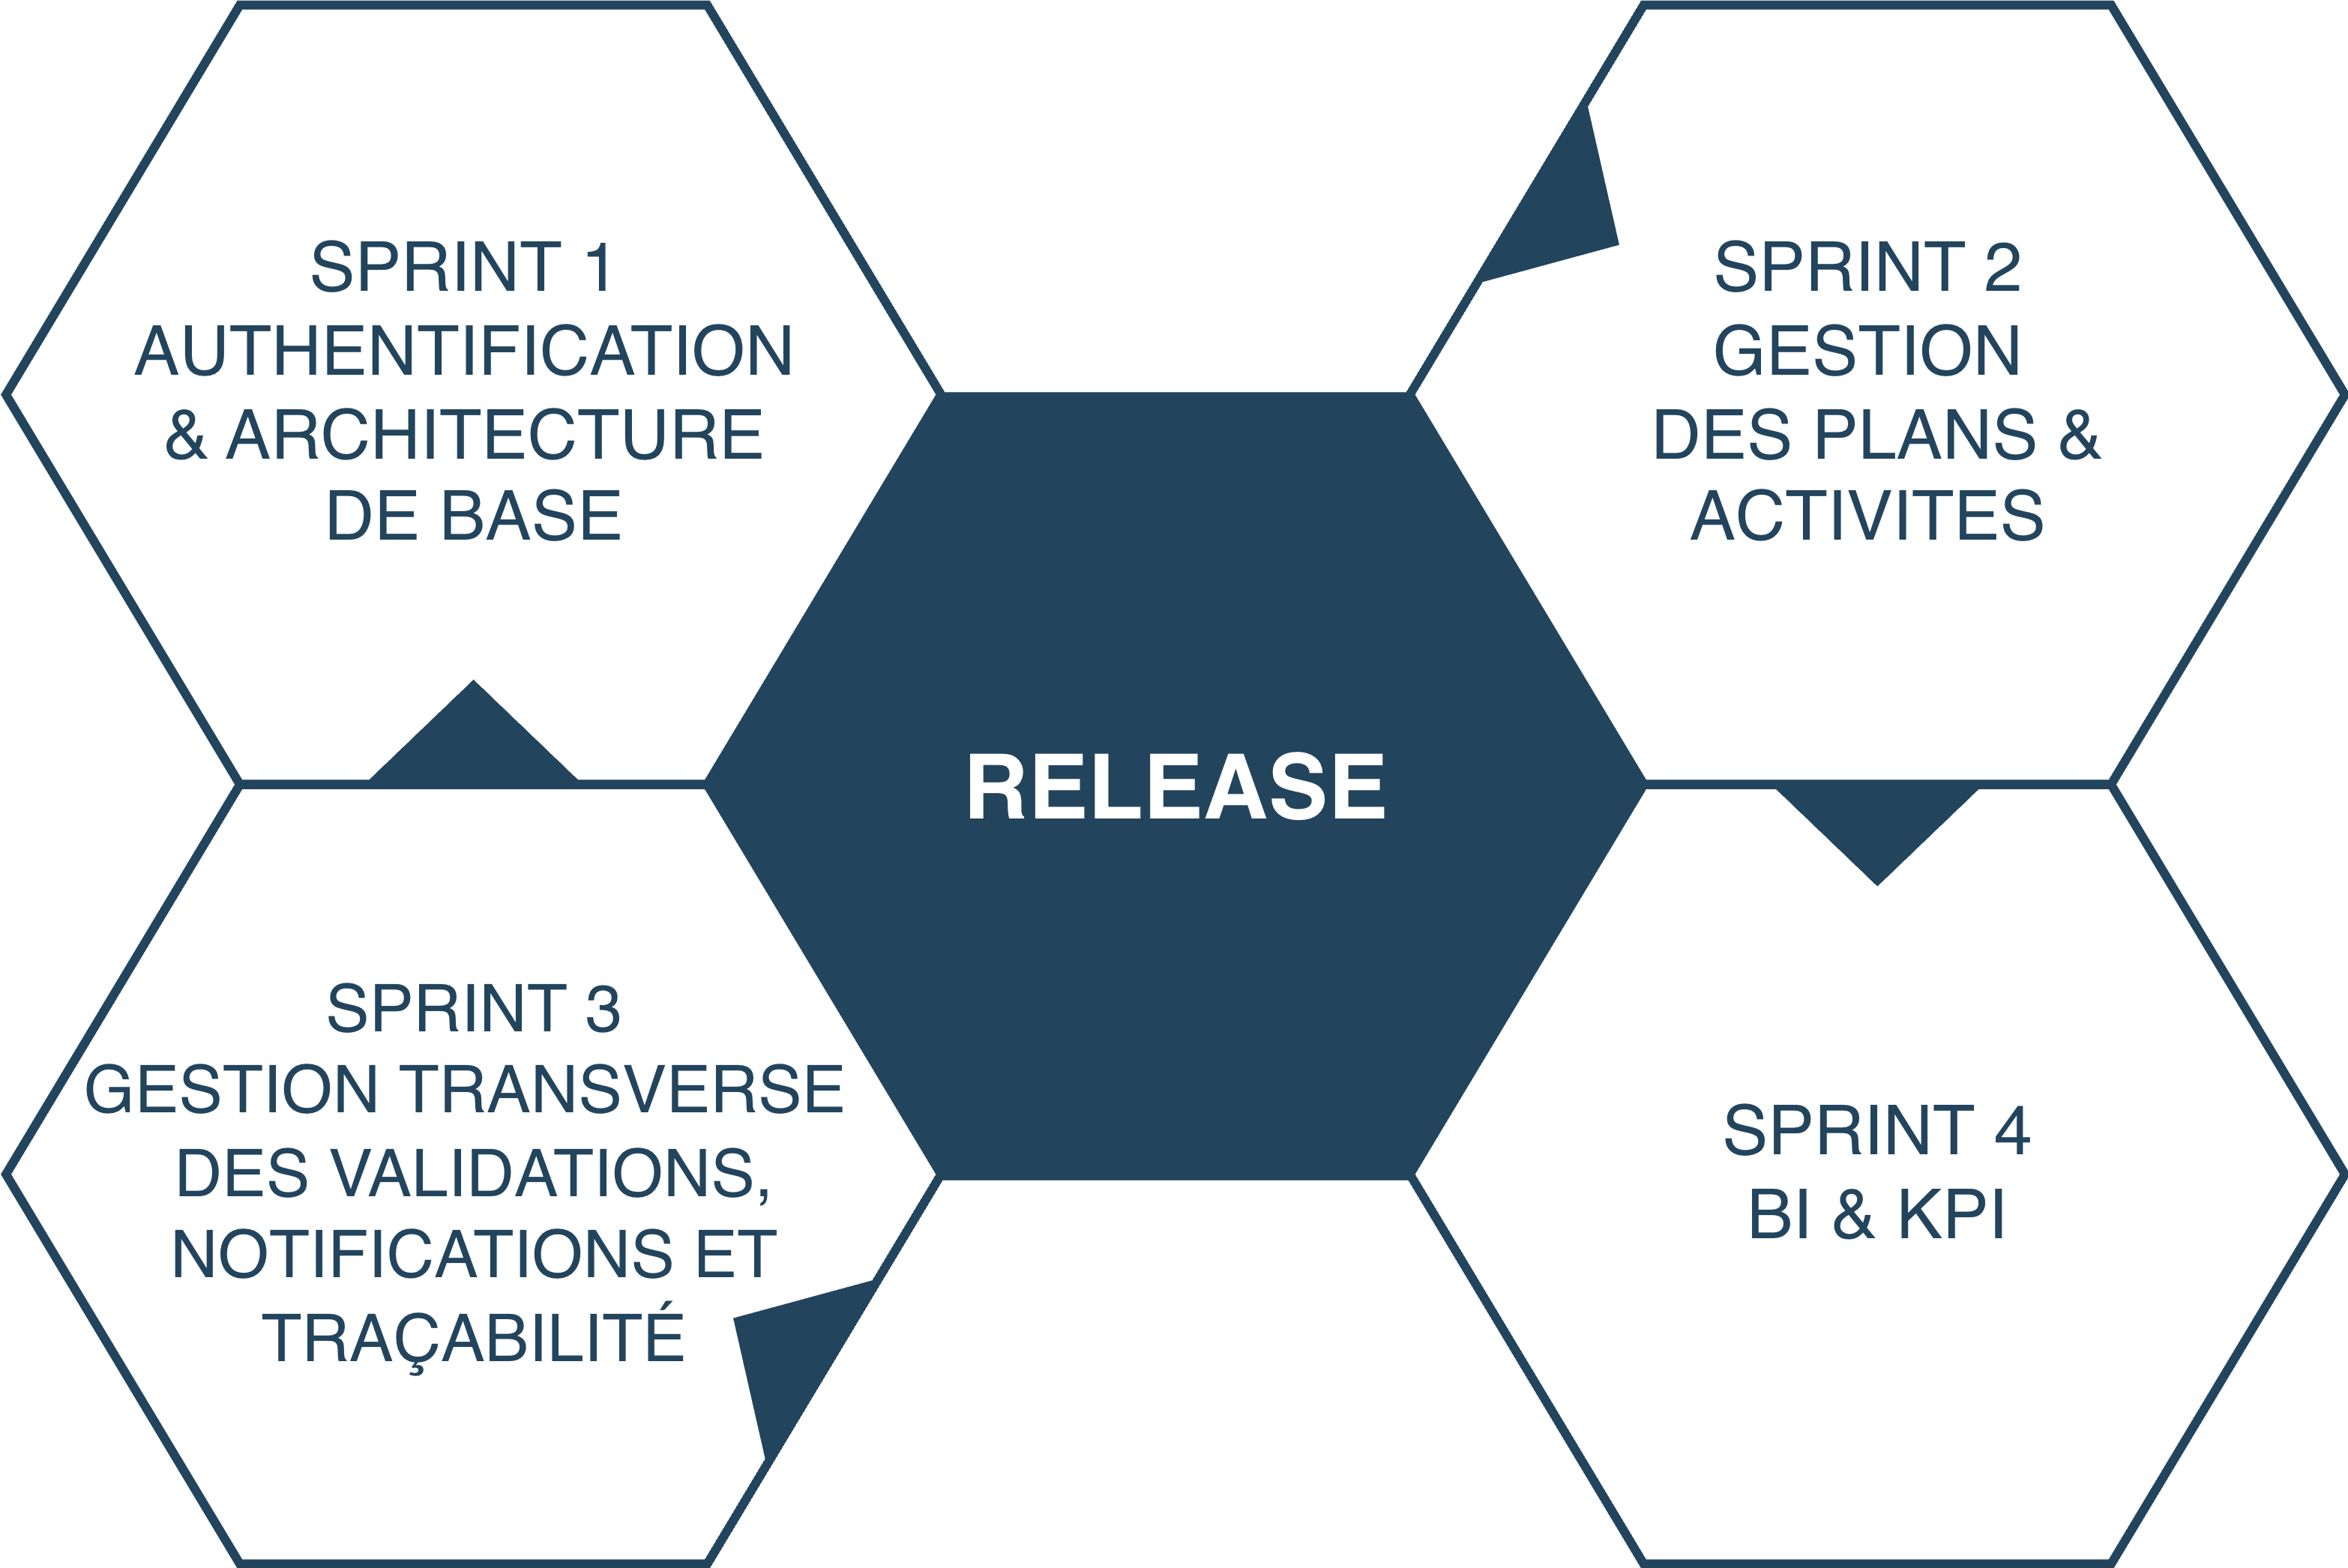
\includegraphics[width=0.9\linewidth]{figures/chapitre-02/Division-du-projet.png}
  \caption{Division du projet en sprints.}
  \label{fig:doc-ch2-division-projet}
\end{figure}

\begin{table}[H]
  \centering
  \small
  \caption{Méthode GIMSI adaptée dans un contexte Scrum.}
  \label{tab:ch02-gimsi-phases}
  \PFETableSetup
  % Tableau plus large que le bloc de texte : déborde de façon symétrique dans les marges.
  \makebox[\textwidth][c]{%
  \begingroup
  \renewcommand{\tabularxcolumn}[1]{>{\raggedright\arraybackslash}m{#1}}%
  \PFETableArrayStretch
  \arrayrulecolor{black}%
  \begin{tabularx}{\dimexpr\PFETableBlockWidth+2.8cm\relax}{%
    |>{\centering\arraybackslash}m{3.1cm}%
    |>{\centering\arraybackslash}m{0.55cm}%
    |>{\raggedright\arraybackslash}m{2.45cm}%
    |>{\raggedright\arraybackslash}X|}%
    \hline
    \tableHeaderStyle
    \tableHeaderCell{Phase} &
    \tableHeaderCell{N\textsuperscript{o}} &
    \tableHeaderCell{Étape} &
    \tableHeaderCell{Adaptation dans Scrum} \\
    \hline
    \multirow{2}{*}{\parbox{3.0cm}{\centering\bfseries Identification}} &
      \textbf{1} & Environnement de l’entreprise &
      Défini progressivement dans le Product Backlog. \\
    \cline{2-4}
    & \textbf{2} & Identification des acteurs &
      Réalisé via les User Stories et échanges avec les parties prenantes. \\
    \hline
    \multirow{5}{*}{\parbox{3.0cm}{\centering\bfseries Conception}} &
      \textbf{3} & Définition des objectifs &
      Affinés à chaque Sprint Planning. \\
    \cline{2-4}
    & \textbf{4} & Construction du tableau de bord &
      Conception itérative avec retour utilisateur. \\
    \cline{2-4}
    & \textbf{5} & Choix des indicateurs &
      KPI ajustés selon les besoins métiers évolutifs. \\
    \cline{2-4}
    & \textbf{6} & Collecte des informations &
      Données intégrées progressivement. \\
    \cline{2-4}
    & \textbf{7} & Système de tableaux de bord &
      Amélioration continue des tableaux de bord. \\
    \hline
    \multirow{2}{*}{\parbox{3.0cm}{\centering\bfseries Mise en œuvre}} &
      \textbf{8} & Choix des outils &
      Power BI retenu selon les besoins du projet. \\
    \cline{2-4}
    & \textbf{9} & Intégration &
      Réalisé par incréments à chaque sprint. \\
    \hline
    \parbox{3.0cm}{\centering\bfseries Suivi permanent} &
      \textbf{10} & Audit et amélioration &
      Amélioration continue via retours et itérations Scrum. \\
    \hline
  \end{tabularx}%
  \endgroup
  }%
\end{table}


\subsection{Planification des Sprints}

Après finalisation du \emph{product backlog}, nous avons estimé l’effort et le temps requis pour chaque élément et regroupé ceux-ci en phases de développement cohérentes. Le projet a été découpé en \textbf{quatre sprints}, chacun visant un ensemble de fonctionnalités du backlog avec une durée définie.

Le tableau~\ref{tab:ch02-planification-sprints} synthétise cette planification.

\begin{table}[H]
  \centering
  \small
  \caption{Planification du projet par sprints.}
  \label{tab:ch02-planification-sprints}
  \PFETableSetup
  \PFETableRowColors
  \PFETableArrayStretch
  \arrayrulecolor{black}
  \PFETableTabularXBegin
  \begin{tabularx}{\textwidth}{@{}>{\centering\arraybackslash}p{0.95cm}>{\raggedright\arraybackslash}p{2.35cm}>{\raggedright\arraybackslash}X>{\centering\arraybackslash}p{1.95cm}@{}}
    \hline
    \tableHeaderStyle
    \tableHeaderCell{N\textsuperscript{o}} &
    \tableHeaderCell{Nom du sprint} &
    \tableHeaderCell{Fonctionnalités couvertes} &
    \tableHeaderCell{Durée} \\
    \hline
    1 &
    Authentification \& Fondations &
    \begin{minipage}[t]{\linewidth}
      \begin{itemize}[leftmargin=*, itemsep=0.15ex, parsep=0pt, topsep=0.5pt, partopsep=0.5pt, label=\textbullet]
        \item Accès, rôles, cloisonnement (1)
        \item Fichiers (8)
        \item Référentiel entreprise/sites et documents (US\,1.4--1.5)
      \end{itemize}
    \end{minipage} &
    4 semaines \\
    \hline

    2 &
    Plans \& activités &
    \begin{minipage}[t]{\linewidth}
      \begin{itemize}[leftmargin=*, itemsep=0.15ex, parsep=0pt, topsep=0pt, partopsep=0pt, label=\textbullet]
        \item Plan annuel (2)
        \item Activités (3)
        \item Hors plan, indicateurs, pièces jointes, validation (5)
        \item Écarts planifié/réalisé et pilotage
      \end{itemize}
    \end{minipage} &
    4 semaines \\
    \hline
    3 &
    Workflow transverse &
    \begin{minipage}[t]{\linewidth}
      \begin{itemize}[leftmargin=*, itemsep=0.15ex, parsep=0pt, topsep=0pt, partopsep=0pt, label=\textbullet]
        \item Validation (2--3)
        \item Demandes de modification (4)
        \item Notifications (7)
        \item Chatbot (9)
        \item Tâches (11)
        \item Traçabilité (US\,2.7, 4.4)
      \end{itemize}
    \end{minipage} &
    4 semaines \\
    \hline
    4 &
    BI \& KPI &
    \begin{minipage}[t]{\linewidth}
      \begin{itemize}[leftmargin=*, itemsep=0.15ex, parsep=0pt, topsep=0pt, partopsep=0pt, label=\textbullet]
        \item Dashboards (5)
        \item Power BI (6)
        \item KPI et GIMSI (10)
      \end{itemize}
    \end{minipage} &
    3 semaines \\
    \hline
  \end{tabularx}
  \PFETableTabularXEnd
\end{table}



\subsection{Diagramme de classe générale}

La figure~\ref{fig:doc-ch2-3} illustre le diagramme de classe général de la solution. Le dictionnaire de données détaillant les attributs de ce schéma est fourni en annexe~B (tableau~\ref{tab:dictionnaire-donnees-classe}).

\clearpage
\newgeometry{margin=0pt}
\begin{landscape}
  \begingroup
  % Page dédiée au diagramme (sans footer/numéro/logo) + image au maximum de la page.
  \pagestyle{empty}
  \thispagestyle{empty}
  \captionsetup{aboveskip=2pt,belowskip=0pt,font=small}
  \begin{figure}[p]
    \thispagestyle{empty}
    \centering
    \includegraphics[
      width=1.3\paperwidth,
      height=\paperheight,
      keepaspectratio
    ]{figures/chapitre-02/diagramme-classe-general.png}
    \caption{Diagramme de classe général.}
    \label{fig:doc-ch2-3}
  \end{figure}
  \endgroup
\end{landscape}
\restoregeometry
\clearpage
\section{Architecture du système}

L’architecture de la plateforme est conçue pour orchestrer la création, la validation et l’exploitation des données CSR de manière sécurisée. Après authentification, le flux principal se divise en deux branches.
\par\addvspace{2ex}%

L’architecture repose sur une approche en couches permettant d’assurer une séparation claire des responsabilités et une meilleure maintenabilité du système. Elle s’organise autour de plusieurs niveaux : la couche de présentation, la couche d’authentification, la couche applicative, la couche de données opérationnelles et la couche décisionnelle.
\par\addvspace{2ex}%
Au niveau de la couche de présentation, l’utilisateur interagit avec une application web développée en Angular. L’accès aux fonctionnalités est sécurisé grâce à un mécanisme d’authentification basé sur des tokens JWT, géré par une API Flask dédiée.
\par\addvspace{2ex}%
La couche applicative est assurée par une API REST développée avec Flask, structurée en plusieurs modules métiers (plans, activités, workflow, documents, audit). Cette couche implémente la logique métier du système, notamment la validation des données, la gestion des droits d’accès et le pilotage des processus de workflow.
\par\addvspace{2ex}% 
Les données sont ensuite persistées dans une base de données MySQL via une couche ORM\footnote{ORM : \emph{Object-Relational Mapping} (mapping objet-relationnel). Il s’agit d’une approche de persistance qui met en correspondance les objets manipulés dans le code applicatif et les enregistrements d’une base relationnelle, afin de structurer les accès aux données et de limiter le SQL ad hoc~\cite{orm-wikipedia}. Dans ce projet, cette couche est assurée par SQLAlchemy et Flask-SQLAlchemy~\cite{sqlalchemy-docs}.}
, garantissant une abstraction efficace entre l’application et la base de données. Les fichiers et documents associés sont stockés dans un espace de stockage dédié.
\par\addvspace{2ex}%
Par ailleurs, la plateforme intègre un mécanisme de communication en temps réel via Socket.IO, permettant la diffusion instantanée des notifications et des mises à jour vers l’interface utilisateur.
\par\addvspace{2ex}%

Enfin, une couche décisionnelle vient compléter l’architecture. Les données issues de la base opérationnelle sont extraites, transformées et chargées via SSIS vers un Data Warehouse. Ce dernier est exploité à l’aide de SSMS pour la modélisation et l’analyse, puis connecté à Power BI pour la création de tableaux de bord interactifs et avancés. Cette séparation entre les systèmes transactionnels (OLTP) et analytiques (OLAP) permet d’optimiser les performances globales et de faciliter la prise de décision.

La figure~\ref{fig:doc-ch2-system-architecture} illustre l'architecture globale du système.

\begin{figure}[H]
  \centering
  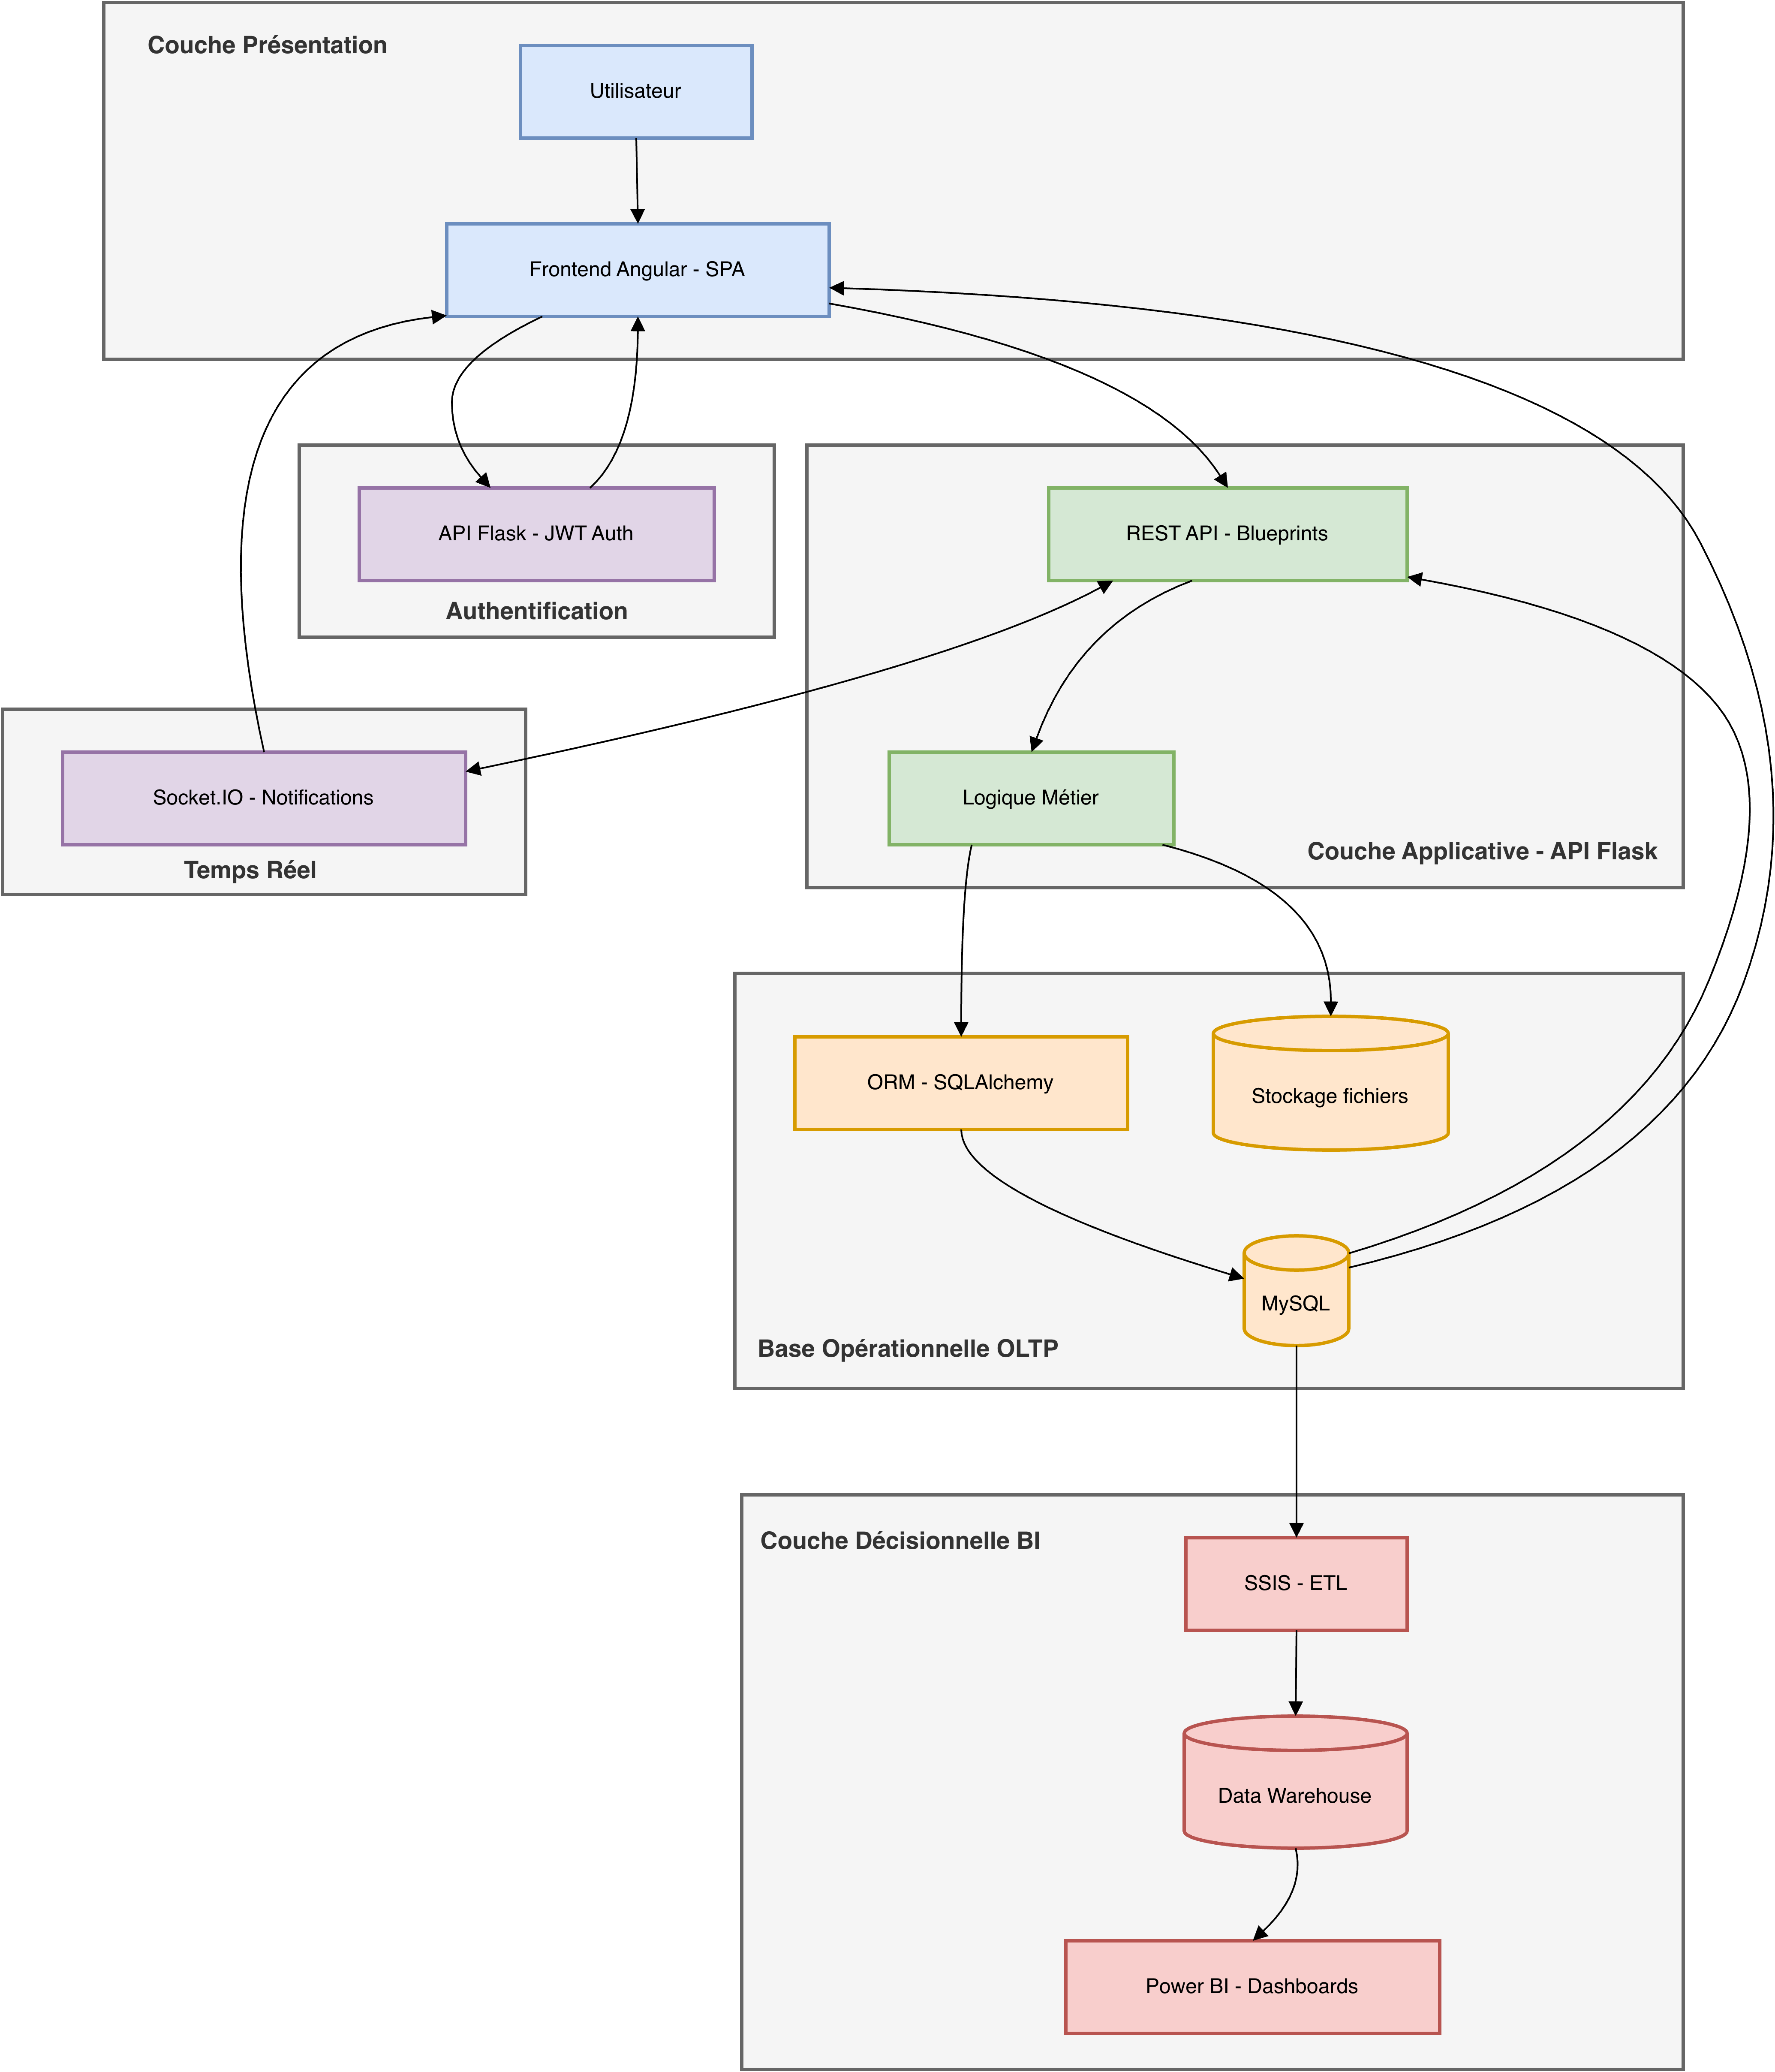
\includegraphics[width=\linewidth]{figures/chapitre-02/architecture-systeme-csr.png}
  \caption{Architecture globale du système.}
  \label{fig:doc-ch2-system-architecture}
\end{figure}
\footnote{SSIS : \emph{SQL Server Integration Services}. Il s’agit de la composante ETL (\emph{Extract, Transform, Load}) de SQL Server permettant de concevoir des flux d’intégration entre sources de données hétérogènes, de transformer et charger des données, puis d’orchestrer et de déployer ces traitements sous forme de packages~\cite{ssis-docs}.}
\footnote{SSMS : \emph{SQL Server Management Studio}. Il s’agit de l’outil graphique fourni par Microsoft pour administrer une instance SQL Server : exécution de requêtes T-SQL, gestion des bases et des schémas, configuration de la sécurité, sauvegardes et surveillance~\cite{ssms-docs}.}
\section{Choix des technologies}

Dans le cadre du développement de notre projet, nous avons retenu une pile technologique répondant aux exigences de \textbf{performance}, de \textbf{sécurité} (authentification, contrôle d’accès, cloisonnement par site) et de \textbf{scalabilité}. Chaque technologie a été choisie pour un rôle précis afin d’assurer une implémentation robuste et une maintenance aisée.


\subsection{Backend}

\vspace{0.35em}
\textbf{Python }\cite{python-docs} est un langage de programmation polyvalent, largement utilisé pour le développement web et l’intégration de services. 

La figure~\ref{fig:doc-ch2-tech-python-logo} présente le logo officiel de Python.
\begin{figure}[H]
  \centering
  
\includegraphics[height=1.8cm]{figures/chapitre-02/python.png}
  \caption[Logo de Python.]{Logo de Python.}
  \label{fig:doc-ch2-tech-python-logo}
\end{figure}

\vspace{0.35em}
\textbf{Flask }\cite{flask-docs} est un micro-framework Python \emph{open source} permettant de développer des applications web et des API REST de façon modulaire (blueprints, extensions). 

La figure~\ref{fig:doc-ch2-tech-flask-logo} présente le logo officiel de Flask.
\begin{figure}[H]
  \centering
  
\includegraphics[height=1.8cm]{figures/chapitre-02/flask.png}
  \caption[Logo de Flask.]{Logo de Flask.}
  \label{fig:doc-ch2-tech-flask-logo}
\end{figure}

\vspace{0.35em}
\textbf{MySQL}\cite{mysql-docs} est un système de gestion de base de données relationnelle fondé sur SQL, adapté au stockage structuré des entités métier et aux requêtes d’analyse.

La figure~\ref{fig:doc-ch2-tech-mysql-logo} présente le logo officiel de MySQL.
\begin{figure}[H]
  \centering
  
\includegraphics[height=1.8cm]{figures/chapitre-02/MySQL.png}
  \caption[Logo de MySQL.]{Logo de MySQL.}
  \label{fig:doc-ch2-tech-mysql-logo}
\end{figure}

\subsection{Frontend}

\vspace{0.2em}
\textbf{Angular }\cite{angular-docs} est un framework front-end basé sur des composants, proposant routage et injection de dépendances pour structurer une application web. 

La figure~\ref{fig:doc-ch2-tech-angular-logo} présente le logo officiel d’Angular.
\begin{figure}[H]
  \centering
  
\includegraphics[height=1.8cm]{figures/chapitre-02/angular.png}
  \caption[Logo d’Angular.]{Logo d’Angular.}
  \label{fig:doc-ch2-tech-angular-logo}
\end{figure}

\vspace{0.2em}
\textbf{TypeScript }\cite{typescript-docs} est un sur-ensemble typé de JavaScript, améliorant la robustesse du code (typage statique, outillage). 

La figure~\ref{fig:doc-ch2-tech-typescript-logo} présente le logo officiel de TypeScript.
\begin{figure}[H]
  \centering
  
\includegraphics[height=1.8cm]{figures/chapitre-02/TypeScript.png}
  \caption[Logo de TypeScript.]{Logo de TypeScript.}
  \label{fig:doc-ch2-tech-typescript-logo}
\end{figure}

\subsection{Interface utilisateur}

\vspace{0.2em}
\textbf{Tailwind CSS }\cite{tailwind-docs} est un framework utilitaire de styles permettant de composer rapidement des interfaces cohérentes. 

La figure~\ref{fig:doc-ch2-tech-tailwind-logo} présente le logo officiel de Tailwind CSS.
\begin{figure}[H]
  \centering
  
\includegraphics[height=1.8cm]{figures/chapitre-02/tailwind-css.png}
  \caption[Logo de Tailwind CSS.]{Logo de Tailwind CSS.}
  \label{fig:doc-ch2-tech-tailwind-logo}
\end{figure}

\vspace{0.2em}

\subsection{Communication temps réel}

\vspace{0.2em}
\textbf{Socket.IO }\cite{socketio-docs} est une bibliothèque de communication temps réel (événements) reposant sur WebSocket avec mécanismes de repli. 

La figure~\ref{fig:doc-ch2-tech-socketio-logo} présente le logo officiel de Socket.IO.
\begin{figure}[H]
  \centering
  
\includegraphics[height=1.8cm]{figures/chapitre-02/socket-io.png}
  \caption[Logo de Socket.IO.]{Logo de Socket.IO.}
  \label{fig:doc-ch2-tech-socketio-logo}
\end{figure}

\subsection{Outil de test}

\vspace{0.2em}
\textbf{Postman}\cite{postman-docs} est l’outil utilisé pour tester les API REST de la plateforme. Il permet de construire des requêtes, vérifier les réponses (succès/erreur) et valider les scénarios fonctionnels des endpoints backend.

La figure~\ref{fig:doc-ch2-tech-postman-logo} présente le logo de Postman.
\begin{figure}[H]
  \centering
  \IfFileExists{figures/chapitre-02/Postmam.png}{%
    
\includegraphics[height=2.cm]{figures/chapitre-02/Postmam.png}
  }{%
    \fbox{\parbox{4.6cm}{\centering\textit{Logo Postman à insérer}\\\texttt{figures/chapitre-02/Postmam.png}}}
  }
  \caption[Logo de Postman.]{Logo de Postman.}
  \label{fig:doc-ch2-tech-postman-logo}
\end{figure}

\section{Environnement et outils de développement}

Cette section décrit l’\textbf{environnement matériel} et l’\textbf{environnement logiciel} mobilisés pour concevoir, tester et documenter la plateforme.

\subsection{Environnement matériel}

Le développement a été réalisé sur \textbf{deux postes de travail}. 

Le tableau~\ref{tab:ch2-materiel} récapitule leurs caractéristiques principales.

\begin{table}[H]
  \centering
  \small
  \caption{Environnement matériel utilisé pour le développement.}
  \label{tab:ch2-materiel}
  \PFETableSetup
  \PFETableRowColors
  \PFETableArrayStretch
  \begin{tabular}{@{}>{\raggedright\arraybackslash}p{4.2cm}p{5.0cm}p{5.0cm}@{}}
    \tableHeaderStyle \tableHeaderCell{Élément} & \tableHeaderCell{MacBook Pro M1} & \tableHeaderCell{HP Vectus 15} \\
    Processeur (CPU) & M1 8 c\oe urs  & AMD Ryzen 5 5600H \\
    Carte graphique (GPU) & 8 c\oe urs (Apple GPU) & Nvidia GeForce GTX 1650 \\
    Neural Engine & 16 c\oe urs & 16 c\oe urs \\
    Mémoire vive & 8~Go & 24~Go RAM \\
    Stockage & SSD 256~Go & SSD 512~Go \\
    Système d’exploitation & macOS 26.3.1 (Tahoe) & Windows 11 (64 bits) \\
  \end{tabular}
\end{table}

\subsection{Environnement logiciel}

Notre projet s’appuie sur un ensemble d’outils logiciels adaptés aux phases de conception, de développement, de collaboration et de reporting. Chaque outil répond à un besoin précis afin d’assurer une mise en œuvre efficace et une documentation de qualité.

\subsection{Conception et architecture}

\vspace{0.2em}
\textbf{draw.io }\cite{diagrams-net-docs} est un outil de création de diagrammes (schémas d’architecture, diagrammes UML, organigrammes) avec export vers plusieurs formats. 

La figure~\ref{fig:doc-ch2-drawio-logo} présente le logo officiel de draw.io.

\begin{figure}[H]
  \centering
  
\includegraphics[height=1.4cm]{figures/chapitre-02/draw-io.png}
  \caption[Logo de draw.io.]{Logo de draw.io.}
  \label{fig:doc-ch2-drawio-logo}
\end{figure}

\subsection{Gestion de versions et collaboration}

\vspace{0.2em}
\textbf{Git }\cite{git-docs} est un système de contrôle de version distribué permettant de suivre l’historique, gérer des branches et faciliter le travail collaboratif. 

La figure~\ref{fig:doc-ch2-git-logo} montre le logo officiel de Git.
\begin{figure}[H]
  \centering
  
\includegraphics[height=1.4cm]{figures/chapitre-02/Git.png}
  \caption[Logo de Git.]{Logo de Git.}
  \label{fig:doc-ch2-git-logo}
\end{figure}

\vspace{0.2em}
\textbf{GitHub }\cite{github-docs} est une plateforme d’hébergement de dépôts Git offrant des fonctionnalités de collaboration (issues, pull requests, revue de code). 

La figure~\ref{fig:doc-ch2-github-logo} montre le logo officiel de GitHub.
\begin{figure}[H]
  \centering
  
\includegraphics[height=1.4cm]{figures/chapitre-02/github.png}
  \caption[Logo de GitHub.]{Logo de GitHub.}
  \label{fig:doc-ch2-github-logo}
\end{figure}

\vspace{0.2em}
\textbf{Monday.com }\cite{monday-docs} est un outil de gestion de projet et de travail collaboratif basé sur des tableaux visuels, facilitant l’organisation des tâches, le suivi de l’avancement et la coordination des équipes.

La figure~\ref{fig:doc-ch2-monday-logo} présente le logo officiel de Monday.com.
\begin{figure}[H]
  \centering
  
\includegraphics[width=8cm]{figures/chapitre-02/Monday_logo.svg.png}
  \caption[Logo de Monday.com.]{Logo de Monday.com.}
  \label{fig:doc-ch2-monday-logo}
\end{figure}

\subsection{Développement}

\vspace{0.2em}
\textbf{Visual Studio Code }\cite{vscode-docs} est un éditeur de code extensible et multiplateforme proposant notamment l’auto-complétion, le débogage et l’intégration Git. 

La figure~\ref{fig:doc-ch2-vscode-logo} présente le logo officiel de Visual Studio Code.
\begin{figure}[H]
  \centering
  
\includegraphics[height=3cm]{figures/chapitre-02/visual-studio-code.jpeg}
  \caption[Logo de Visual Studio Code.]{Logo de Visual Studio Code.}
  \label{fig:doc-ch2-vscode-logo}
\end{figure}

\vspace{0.2em}
\textbf{Microsoft Visual Studio } \cite{visualstudio-docs} est un environnement de développement intégré (IDE) permettant de concevoir, compiler, tester et déboguer des applications. 

La figure~\ref{fig:doc-ch2-visualstudio-logo} présente le logo officiel de Microsoft Visual Studio.
\begin{figure}[H]
  \centering
  
\includegraphics[height=1.4cm]{figures/chapitre-02/Microsoft-Visual-Studio.png}
  \caption[Logo de Microsoft Visual Studio.]{Logo de Microsoft Visual Studio.}
  \label{fig:doc-ch2-visualstudio-logo}
\end{figure}

\vspace{0.2em}
\textbf{Microsoft SQL Server } \cite{sqlserver-docs} est un système de gestion de base de données relationnelle (SGBDR) développé par Microsoft, destiné au stockage et à l’analyse de données. 

La figure~\ref{fig:doc-ch2-sqlserver-logo} présente le logo officiel de Microsoft SQL Server.
\begin{figure}[H]
  \centering
  
\includegraphics[height=1.4cm]{figures/chapitre-02/sql-serveur.png}
  \caption[Logo de Microsoft SQL Server.]{Logo de Microsoft SQL Server.}
  \label{fig:doc-ch2-sqlserver-logo}
\end{figure}

\vspace{0.2em}
\textbf{Mapping objet-relationnel (ORM)} \cite{orm-wikipedia} désigne une approche de persistance qui établit une correspondance entre les objets manipulés dans le code applicatif et les tables (ou vues) d’une base relationnelle, afin de structurer les accès aux données et de réduire le SQL répétitif. Dans le backend de la plateforme CSR, cette couche est assurée par \textbf{SQLAlchemy} \cite{sqlalchemy-docs} (avec Flask-SQLAlchemy comme pont vers l’API Flask). 

La figure~\ref{fig:doc-ch2-sqlalchemy-logo} présente le logo de SQLAlchemy.
\begin{figure}[H]
  \centering
  
\includegraphics[height=1.4cm]{figures/chapitre-02/sqlalchemy.png}
  \caption[Logo de SQLAlchemy (ORM et accès SQL).]{Logo de SQLAlchemy (ORM et accès SQL).}
  \label{fig:doc-ch2-sqlalchemy-logo}
\end{figure}

\vspace{0.2em}
\textbf{XAMPP }\cite{xampp-docs} est une distribution regroupant un serveur web (Apache) et des composants associés (dont MySQL/MariaDB et PHP), utilisée pour mettre en place rapidement un environnement serveur local. 

La figure~\ref{fig:doc-ch2-xampp-logo} montre le logo officiel de XAMPP.
\begin{figure}[H]
  \centering
  
\includegraphics[height=1.4cm]{figures/chapitre-02/Xampp.png}
  \caption[Logo de XAMPP.]{Logo de XAMPP.}
  \label{fig:doc-ch2-xampp-logo}
\end{figure}

\subsection{Reporting et documentation}

\vspace{0.2em}
\textbf{Power BI }\cite{powerbi-docs} est une plateforme de \emph{business intelligence} permettant de créer des rapports et tableaux de bord interactifs. 

La figure~\ref{fig:doc-ch2-powerbi-logo} montre le logo officiel de Power BI.
\begin{figure}[H]
  \centering
  
\includegraphics[height=1.8cm]{figures/chapitre-02/power-bi.png}
  \caption[Logo de Power BI.]{Logo de Power BI.}
  \label{fig:doc-ch2-powerbi-logo}
\end{figure}

\vspace{0.2em}
\textbf{LaTeX } \cite{latex-docs} est un système de composition de documents basé sur \TeX, permettant de produire des documents structurés avec une typographie stable. 

La figure~\ref{fig:doc-ch2-latex-logo} présente le logo officiel de \LaTeX.
\begin{figure}[H]
  \centering
  
\includegraphics[height=1.8cm]{figures/chapitre-02/LaTeX_project_logo_bird.png}
  \caption[Logo de \LaTeX.]{Logo de \LaTeX.}
  \label{fig:doc-ch2-latex-logo}
\end{figure}

\section{Conclusion}

Ce chapitre a posé les bases du projet : exigences fonctionnelles, démarche Scrum, formalisation du \emph{product backlog} et des \emph{user stories}, planification et chronologie des sprints, puis architecture et choix technologiques. Les environnements matériel et logiciel mobilisés pour concevoir la plateforme CSR ont également été décrits. Les chapitres suivants présentent successivement les quatre sprints retenus — \emph{Authentification \& Fondations}, \emph{Plans \& activités}, \emph{Workflow transverse}, \emph{BI \& KPI} — et leur mise en œuvre.


% Importé depuis Chapitre 1 Draft.docx (partie 3) — titre de chapitre inchangé côté \PFEChapterOpening
\PFEChapterOpening{Sprint 1 - Authentification \& Architecture de base}

\section{Introduction}
Ce chapitre présente le premier sprint du projet, qui consiste à poser les bases du système. Il inclut la gestion des accès, des utilisateurs, des sites et des documents.Nous y décrivons les fonctionnalités développées, les choix de conception ainsi que les modèles UML utilisés. Des captures d’écran et une phase de test permettent également de montrer le fonctionnement des éléments réalisés.

\section{Objectif attendu}

Ce premier sprint a pour objectif de mettre en place les fondations du système à travers le développement du module d’authentification et de gestion des accès. Il vise à garantir un accès sécurisé à la plateforme tout en assurant une gestion structurée des utilisateurs selon leurs rôles (site ou corporate). Ce module permettra de contrôler efficacement les droits d’accès, d’isoler les données propres à chaque site et d’offrir une expérience utilisateur adaptée, où chaque acteur interagit uniquement avec les informations qui le concernent. Ainsi, cette étape constitue une base essentielle pour assurer la fiabilité, la sécurité et la cohérence du reste du système.

\section{Sprint Backlog}

Le Sprint Backlog regroupe l'ensemble des fonctionnalités retenues depuis le Product Backlog pour être développées au cours de ce sprint. Il constitue une vision détaillée et opérationnelle du travail à accomplir, en décomposant chaque fonctionnalité en tâches concrètes et réalisables.

Le tableau~\ref{tab:sprint-backlog-1} présente le backlog du premier sprint.

% --- Sprint backlog — même style que product backlog + colonnes alignées sur chapitre 4 ---
% Contenu aligné sur le tableau Word « Tableau 3.1 : Sprint backlog du sprint 1 » (Chapitre 1 Draft).
\small
\PFETableSetup

\setlength{\PFEbacklogTabW}{\dimexpr\textwidth+2.8cm\relax}
\setlength{\LTcapwidth}{\PFEbacklogTabW}
\setlength{\LTleft}{\fill}
\setlength{\LTright}{\fill}

\setlength{\LTpre}{0pt}
\setlength{\LTpost}{0pt}

\PFETableArrayStretch
\setlength{\extrarowheight}{4pt}
\renewcommand{\arraystretch}{1.4}

\arrayrulecolor{black}

\begin{longtable}{|
>{\centering\arraybackslash}m{1.2cm}|
>{\raggedright\arraybackslash}m{5.2cm}|
>{\centering\arraybackslash}m{1.6cm}|
>{\raggedright\arraybackslash}m{5.5cm}|
>{\centering\arraybackslash}m{1.7cm}|}

\caption{Sprint backlog — Authentification \& Architecture de base}\label{tab:sprint-backlog-1}\\

\hline
\tableHeaderStyle
\tableHeaderCell{ID} & \tableHeaderCell{User story} & \tableHeaderCell{Tâche ID} & \tableHeaderCell{Tâche} & \tableHeaderCell{Priorité} \\
\hline
\endfirsthead

\hline
\multicolumn{5}{|c|}{\tablename\ \thetable{} — \textit{(suite)}} \\
\hline
\tableHeaderStyle
\tableHeaderCell{ID} & \tableHeaderCell{User story} & \tableHeaderCell{Tâche ID} & \tableHeaderCell{Tâche} & \tableHeaderCell{Priorité} \\
\hline
\endhead

\hline
\multicolumn{5}{|r|}{\textit{Suite page suivante\ldots}} \\
\hline
\endfoot

\hline
\endlastfoot

1 & En tant qu'utilisateur (Corporate ou Site User), je veux m'authentifier afin d'accéder de manière sécurisée à la plateforme & 1.1 &
Implémenter le module d'authentification & +++++ \\
\cline{3-5}
& & 1.2 &
Vérifier les informations d'identification (email et mot de passe chiffré) & +++++ \\
\cline{3-5}
& & 1.3 &
Générer les tokens d'accès (Access Token et Refresh Token) & +++++ \\
\cline{3-5}
& & 1.4 &
Mettre en place la fonctionnalité de déconnexion avec invalidation du token & +++++ \\
\cline{3-5}
& & 1.5 &
Implémenter le mécanisme de renouvellement des tokens expirés & ++++ \\
\cline{3-5}
& & 1.6 &
Gérer l'expiration de session après inactivité & +++ \\
\hline
2 & En tant qu'utilisateur Corporate, je veux gérer les comptes utilisateurs afin de contrôler l'accès à la plateforme & 2.1 &
Implémenter les fonctionnalités de gestion des utilisateurs & +++++ \\
\cline{3-5}
& & 2.2 &
Ajouter une méthode de création d'un utilisateur avec ses informations & +++++ \\
\cline{3-5}
& & 2.3 &
Ajouter une méthode d'afficher la liste des utilisateurs avec leurs rôles et sites & +++++ \\
\cline{3-5}
& & 2.4 &
Ajouter une méthode de  modification des informations d'un utilisateur & +++++ \\
\cline{3-5}
& & 2.5 &
Ajouter une méthode de désactivation d'un utilisateur & ++++ \\
\cline{3-5}
& & 2.6 &
Ajouter une fonctionnalité de réinitialisation du mot de passe utilisateur & ++++ \\
\cline{3-5}
& & 2.7 &
Ajouter une fonctionnalité de recherche des utilisateurs & ++++ \\
\cline{3-5}
& & 2.8 &
Ajouter une fonctionnalité de filtrage des utilisateurs & ++++ \\
\hline
3 & En tant qu'utilisateur Corporate, je veux attribuer les grades aux utilisateurs afin de gérer leurs permissions d'accès & 3.1 &
Définir les grades principaux (employé, manager) & +++++ \\
\cline{3-5}
& & 3.2 &
Associer un grade à chaque utilisateur & +++++ \\
\cline{3-5}
& & 3.3 &
Ajouter une méthode de  modification du grade d'un utilisateur & ++++ \\
\hline
4 & En tant qu'utilisateur Corporate, je veux sécuriser l'accès aux données en fonction du site afin de garantir la confidentialité des informations & 4.1 &
Implémenter le contrôle d'accès basé sur le site de l'utilisateur & +++++ \\
\cline{3-5}
& & 4.2 &
Restreindre l'accès aux données en fonction du site assigné & +++++ \\
\cline{3-5}
& & 4.3 &
Implémenter des intercepteurs HTTP pour ajouter automatiquement le token aux requêtes & ++++ \\
\cline{3-5}
& & 4.4 &
Gérer les erreurs d'accès (non authentifié, accès refusé) & ++++ \\
\hline
5 & En tant qu'utilisateur, je veux gérer des fichiers afin de documenter les activités CSR & 5.1 &
Implémenter la fonctionnalité d'upload de fichiers & +++++ \\
\cline{3-5}
& & 5.2 &
Gérer les types de fichiers autorisés (PDF, images, Excel) & +++++ \\
\cline{3-5}
& & 5.3 &
Ajouter une méthode de téléchargement des fichiers & ++++ \\
\cline{3-5}
& & 5.4 &
Ajouter une méthode de suppression des fichiers & ++++ \\
\cline{3-5}
& & 5.5 &
Ajouter une méthode de modification des fichiers & ++++ \\
\cline{3-5}
& & 5.6 &
Ajouter une fonctionnalité de consultation des documents & +++++ \\
\cline{3-5}
& & 5.7 &
Ajouter une fonctionnalité de recherche des documents & ++++ \\
\cline{3-5}
& & 5.8 &
Ajouter une fonctionnalité de filtrage des documents & ++++ \\
\cline{3-5}
& & 5.9 &
Ajouter une fonctionnalité de renommage d'un document & ++++ \\
\cline{3-5}
& & 5.10 &
Ajouter une fonctionnalité d'épinglage d'un document & +++ \\
\cline{3-5}
& & 5.11 &
Ajouter une vue des statistiques des fichiers & +++ \\
\cline{3-5}
& & 5.12 &
Ajouter une vue de l'activité récente sur les documents & +++ \\
\hline
6 & En tant qu'utilisateur Corporate, je veux gérer les sites afin d'organiser les activités CSR & 6.1 &
Ajouter une méthode de création d'un site avec ses informations & +++++ \\
\cline{3-5}
& & 6.2 &
Ajouter une méthode de modification des informations d'un site & +++++ \\
\cline{3-5}
& & 6.3 &
Ajouter une méthode de désactivation d'un site & +++++ \\
\cline{3-5}
& & 6.4 &
Associer un utilisateur à un site & +++++ \\
\cline{3-5}
& & 6.5 &
Ajouter une fonctionnalité de consultation d'un site & ++++ \\
\hline
7 & En tant qu'utilisateur, je veux accéder au dashboard afin de consulter une vue synthétique des données & 7.1 &
Implémenter l'accès au dashboard après authentification & +++++ \\
\hline

\end{longtable}

\normalsize


\section{Analyse détaillée des besoins}

\subsection{Diagramme de cas d’utilisation}

La figure~\ref{fig:doc-ch3-1} illustre le diagramme de cas d’utilisation de ce premier sprint.

\begin{figure}[H]
  \centering
  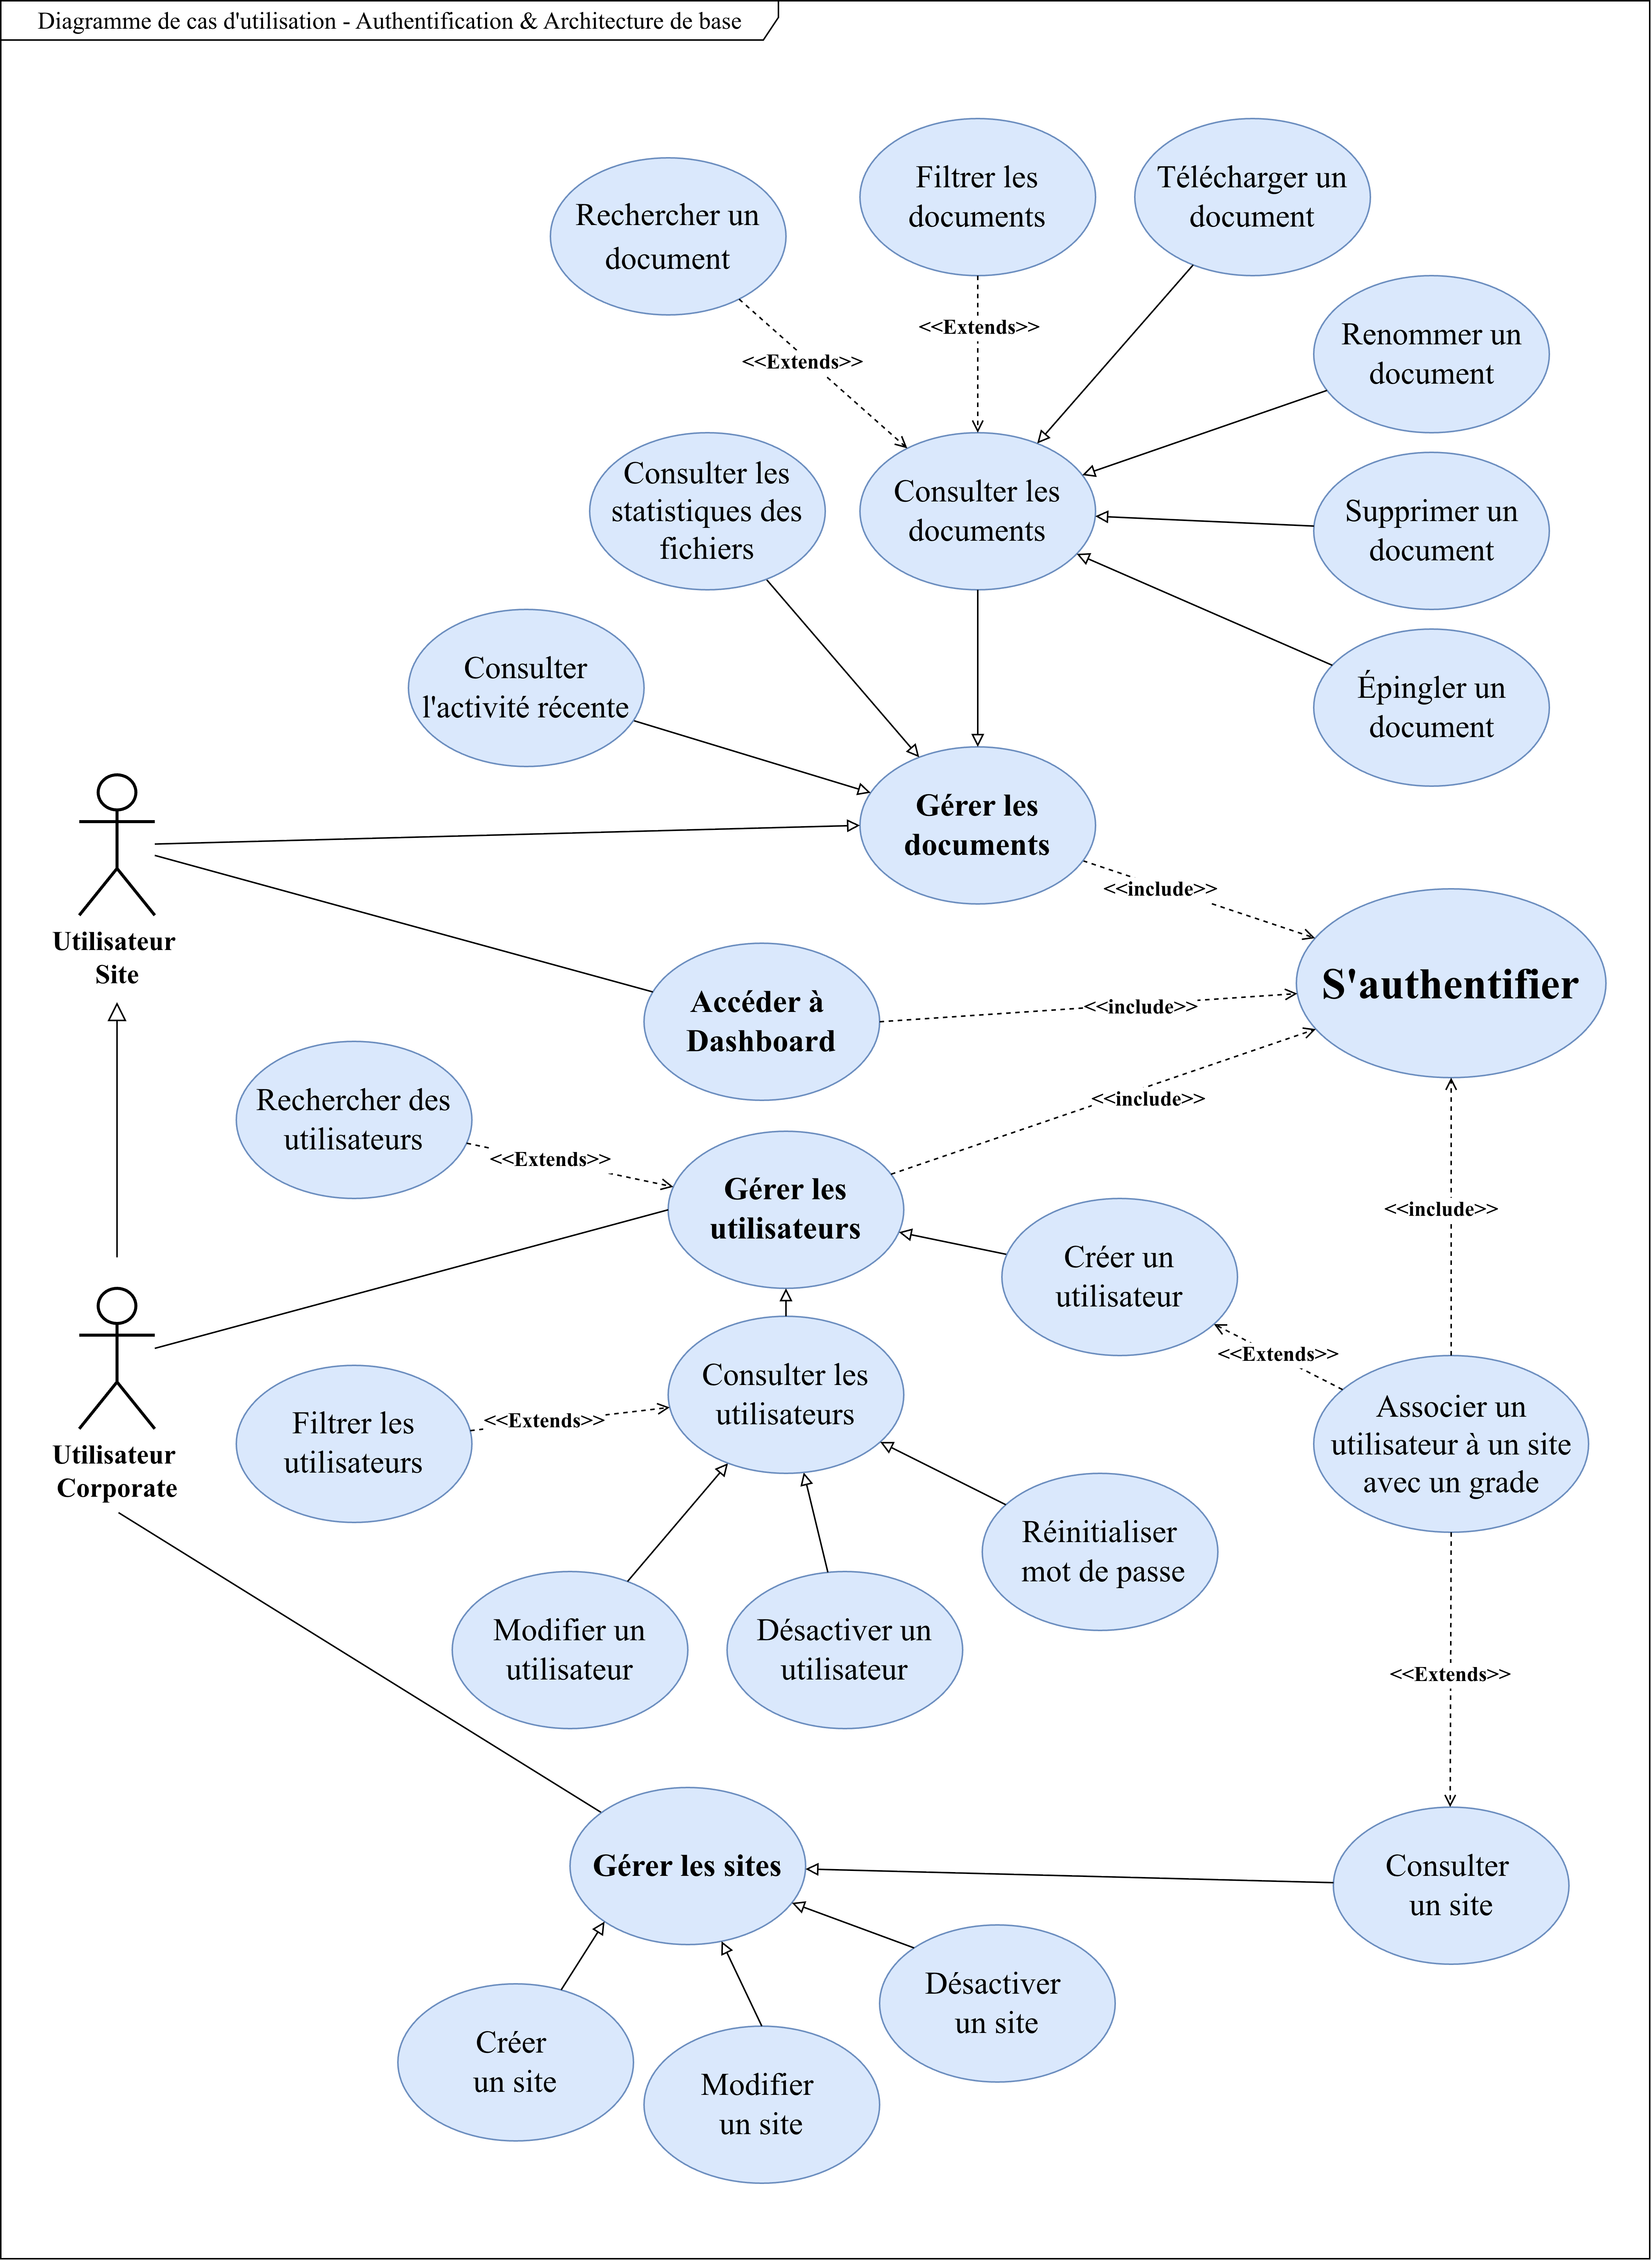
\includegraphics[width=0.92\linewidth]{figures/chapitre-03/diagramme-cas-utilisation-auth-sites-utilisateurs.png}
  \caption{Diagramme de cas d’utilisation — Authentification \& Architecture de base.}
  \label{fig:doc-ch3-1}
\end{figure}

\subsection{Description textuelle du cas d’utilisation : «~Créer un site~»}

Le tableau~\ref{tab:cu-gerer-sites} expose la description textuelle du cas d’utilisation «~Créer un site~».

\begin{table}[H]
  \centering
  \small
  \caption{Description textuelle du cas d’utilisation : «~Créer un site~»}
  \label{tab:cu-gerer-sites}
  \PFETableSetup
  \PFETableRowColors
  \PFETableArrayStretch
  \PFETableTabularXBegin

  \begin{tabularx}{\PFETableBlockWidth}{@{}>{\raggedright\arraybackslash}p{3.2cm} >{\raggedright\arraybackslash}X@{}}
    
    \tableHeaderStyle 
    \tableHeaderCell{Champ} & \tableHeaderCell{Contenu} \\

    \textbf{Titre} & Créer un site \\

    \textbf{Acteurs} & Utilisateur Corporate \\

    \textbf{Objectif} &
    Permettre à l’utilisateur Corporate de créer les sites de Coficab afin d’organiser les activités CSR et structurer l’accès aux données par site. \\

    \textbf{Préconditions} &
    1. L’utilisateur Corporate est authentifié.\par
    2. Un token est obtenu pour accéder aux ressources protégées. \\

    \textbf{Postconditions} &
    1. Les informations du site sont enregistrées.\par
    2. Le nouveau site est disponible pour les autres modules de la plateforme. \\

    \textbf{Scénario nominal} &
    1. L’utilisateur Corporate accède au module de gestion des sites. \par
    2. Le système affiche la liste des sites existants. \par
    3. L’utilisateur choisit l’action : créer un site. \par
    4. L’utilisateur saisit les informations du site (nom, code, pays, région…). \par
    5. Le système valide les données saisies. \par
    6. Si les données sont valides, le système enregistre la création du site et met à jour la liste des sites. \\

    \textbf{Scénario alternatif} &
    \textbf{A. Site déjà existant :} \par
    A.1 L’utilisateur tente de créer un site avec un code déjà existant. \par
    A.2 Le système rejette l’opération. \par
    A.3 Un message est affiché : «~Code site déjà existant~». \\

  \end{tabularx}%

  \PFETableTabularXEnd
\end{table}


\subsection{Description textuelle du cas d’utilisation : «~Créer un utilisateur~»}

Le tableau~\ref{tab:cu-gerer-utilisateurs} expose la description textuelle du cas d’utilisation «~Créer un utilisateur~».

\begin{table}[H]
  \centering
  \small
\caption{Description textuelle du cas d’utilisation : «~Créer un utilisateur~»}
  \label{tab:cu-gerer-utilisateurs}
  \PFETableSetup
  \PFETableRowColors
  \PFETableArrayStretch
  \PFETableTabularXBegin
  \begin{tabularx}{\PFETableBlockWidth}{@{}>{\raggedright\arraybackslash}p{3.2cm} >{\raggedright\arraybackslash}X@{}}
    \tableHeaderStyle \tableHeaderCell{Champ} & \tableHeaderCell{Contenu} \\
    \textbf{Titre} & Créer un utilisateur \\
    \textbf{Acteurs} & Utilisateur Corporate \\
    \textbf{Objectif} &
      Permettre à l’utilisateur Corporate de créer des comptes utilisateurs afin de gérer l’accès à la plateforme. \\
    \textbf{Préconditions} &
      1. L’utilisateur Corporate est authentifié.\par
      2. Un token est obtenu pour accéder aux ressources protégées. \\
    \textbf{Postconditions} &
      1. Les informations du nouvel utilisateur sont enregistrées.\par
      2. Le compte utilisateur est disponible dans la liste des utilisateurs. \\
    \textbf{Scénario nominal} &
      1. L’utilisateur Corporate accède au module de gestion des utilisateurs. \par
      2. Le système affiche la liste des utilisateurs existants. \par
      3. L’utilisateur choisit l’action : créer un utilisateur. \par
      4. L’utilisateur saisit les informations du nouvel utilisateur (nom, email, rôle, site associé, mot de passe…). \par
      5. Le système valide les données saisies. \par
      6. Si les données sont valides, le système enregistre la création de l’utilisateur et met à jour la liste des utilisateurs. \\
    \textbf{Scénario alternatif} &
      \textbf{A. Email déjà utilisé :} \par
      A.1 L’utilisateur Corporate saisit une adresse email déjà existante. \par
      A.2 Le système rejette l’opération. \par
      A.3 Un message est affiché : «~Un utilisateur avec cet email existe déjà~». \par
      \textbf{B. Mot de passe non sécurisé :} \par
      B.1 L’utilisateur Corporate saisit un mot de passe ne respectant pas les critères. \par
      B.2 Le système rejette l’opération. \par
      B.3 Un message est affiché : «~Le mot de passe doit contenir au moins 8 caractères, une majuscule, une minuscule et un caractère spécial~». \\
  \end{tabularx}%
  \PFETableTabularXEnd
\end{table}

\section{Modélisation conceptuelle}

Nous abordons maintenant l'exposé de la conception retenue pour ce premier sprint. À cet effet, nous présentons un diagramme de classe, suivi de la description de plusieurs cas d’utilisation via l'élaboration des diagrammes de séquence appropriés.

\subsection{Diagramme de classe}

Dans le langage UML, le diagramme de classes est un outil essentiel. Il donne une vue claire sur la structure d'un système en décrivant ses classes, leurs attributs, leurs méthodes ainsi que les relations qui les relient entre elles.

La figure~\ref{fig:doc-ch3-2} représente le diagramme de classe du premier sprint.

\begin{figure}[H]
  \centering
  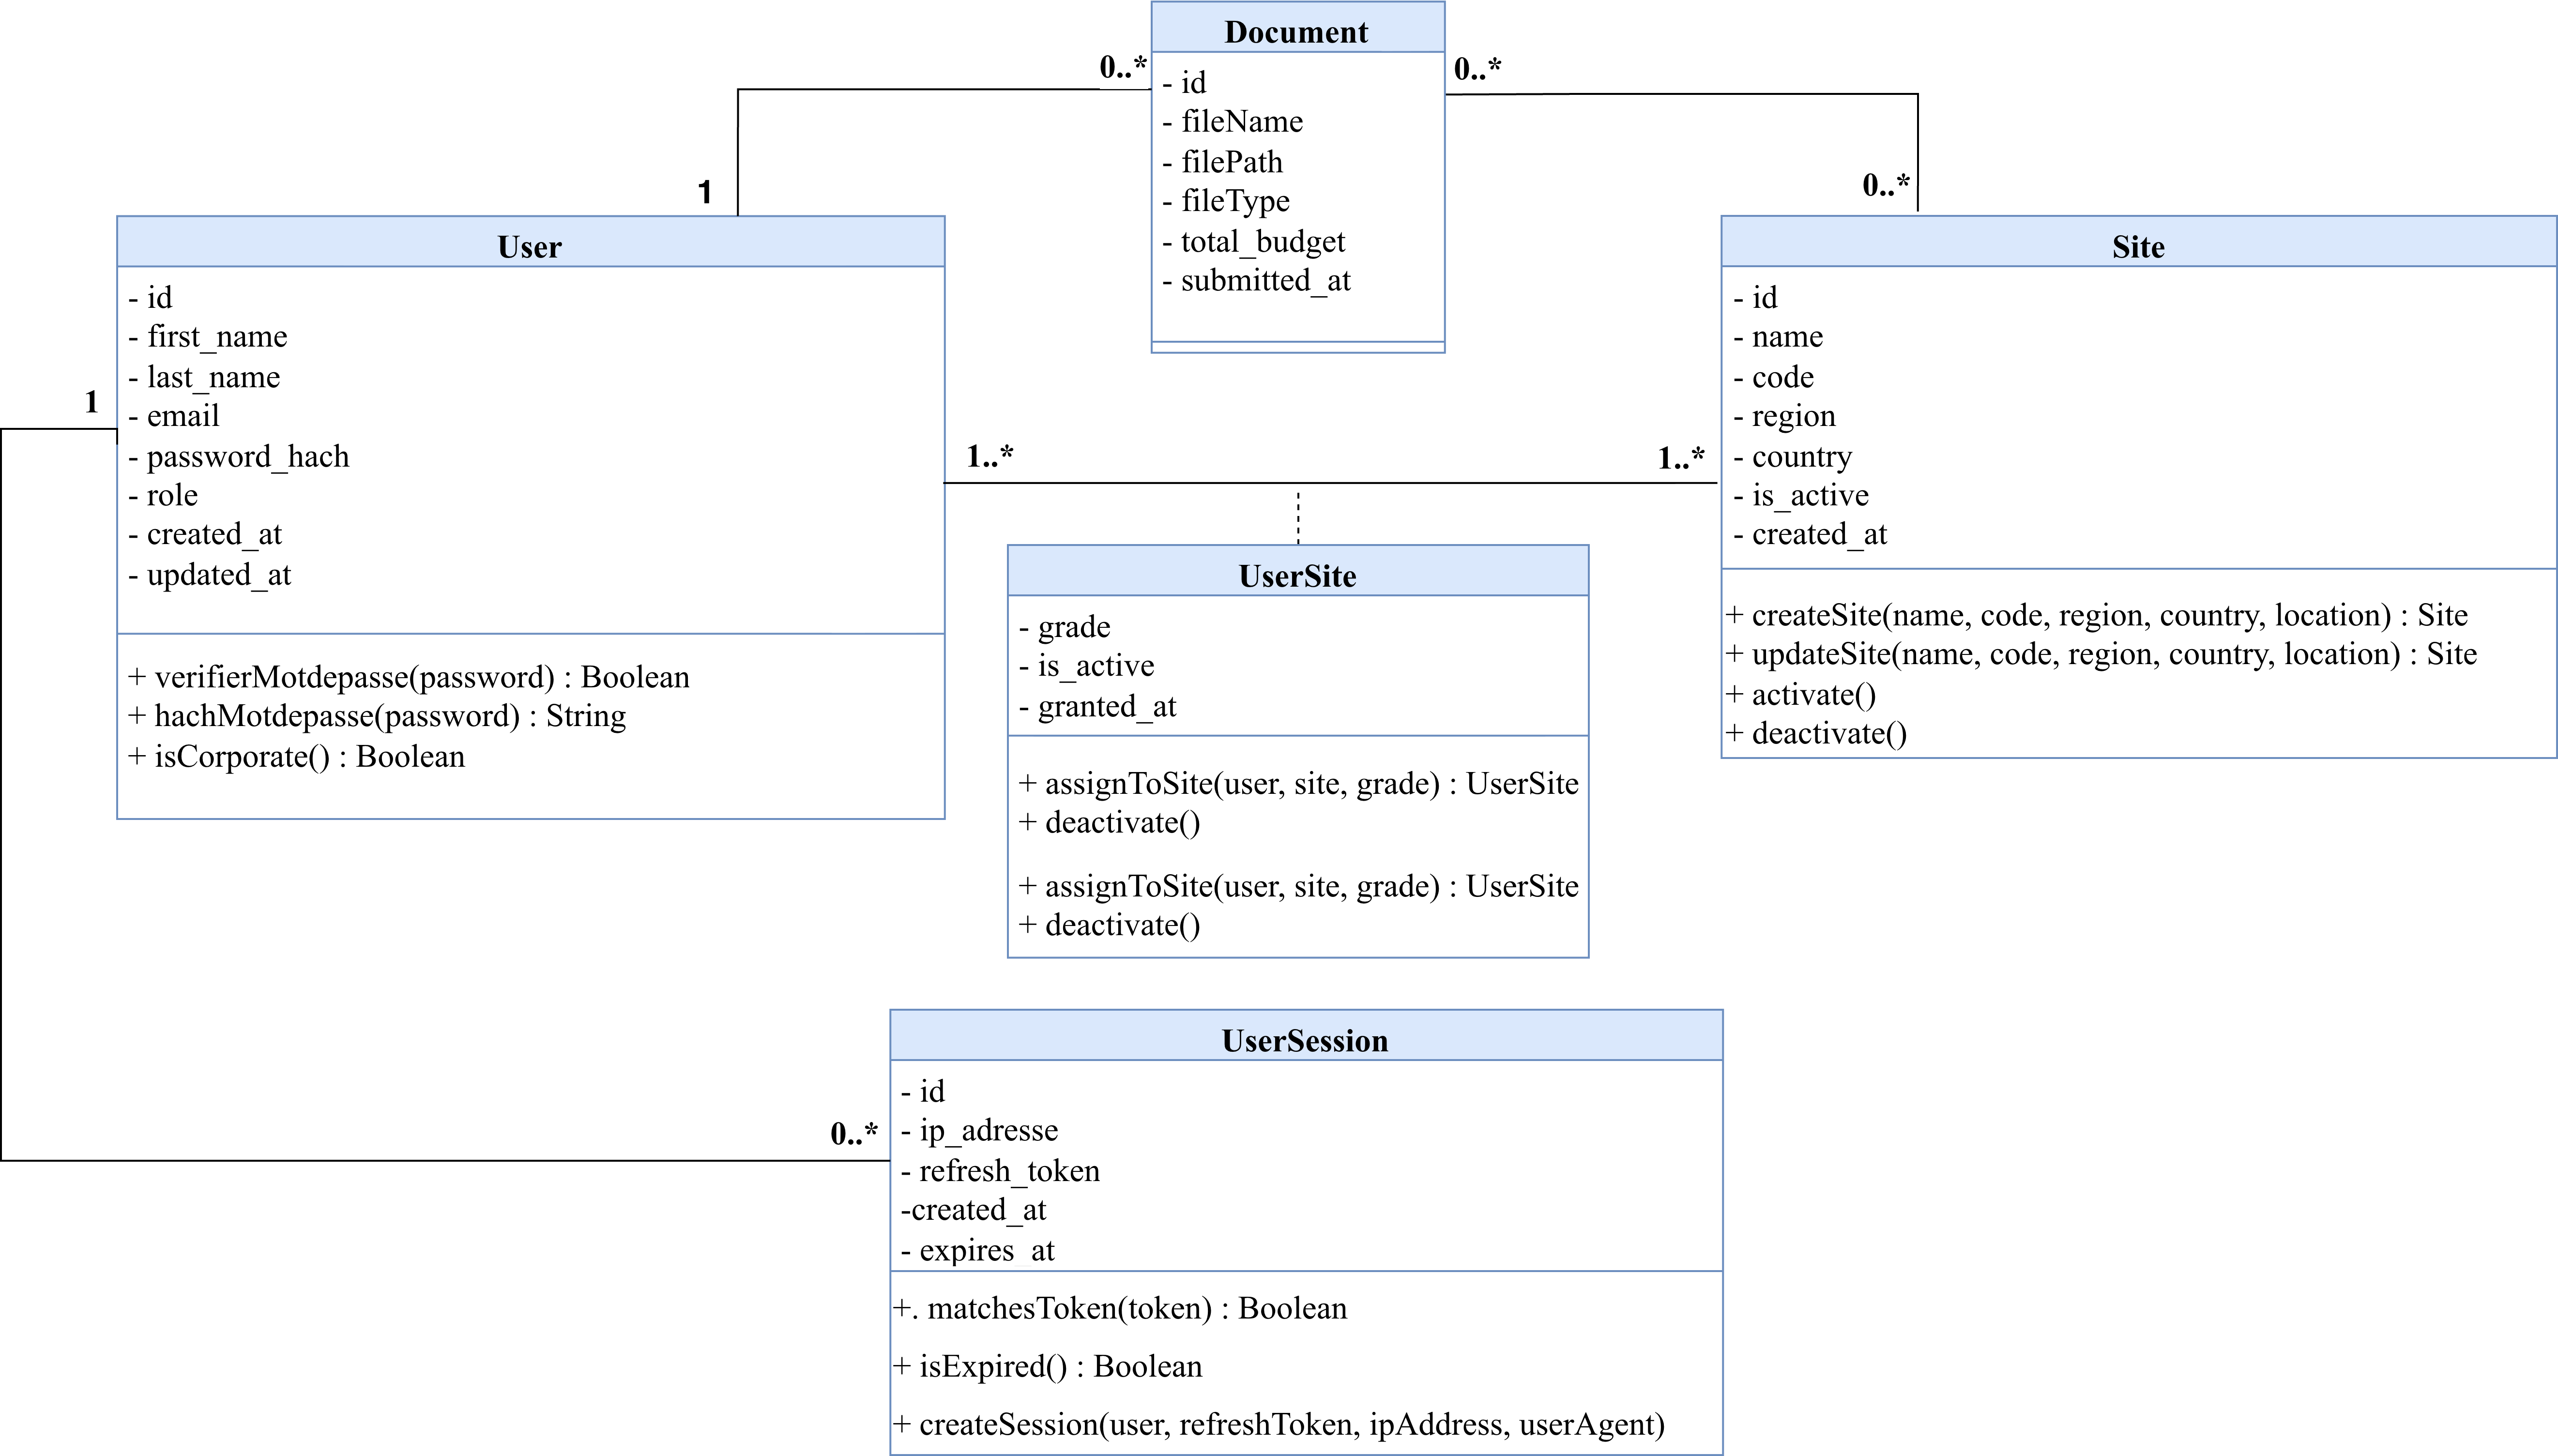
\includegraphics[width=1\linewidth]{figures/chapitre-03/diagramme-classe-auth-sites-documents.png}
  \caption{Diagramme de classe — Authentification \& Architecture de base}
  \label{fig:doc-ch3-2}
\end{figure}

\subsection{Diagramme de séquence}

Les diagrammes de séquences montrent les échanges entre les objets du système. Nous avons documenté les principaux cas d’utilisation du premier sprint : «~S’authentifier~», «~Créer un site~» et «~Créer un utilisateur~».

\subsubsection{Diagramme de séquence : «~S’authentifier~»}

La figure~\ref{fig:doc-ch3-seq-auth} présente le diagramme de séquence du cas d’utilisation «~S’authentifier~».

\IfFileExists{figures/chapitre-03/diagramme-sequence-s-authentifier.png}{%
\begin{figure}[H]
  \centering
  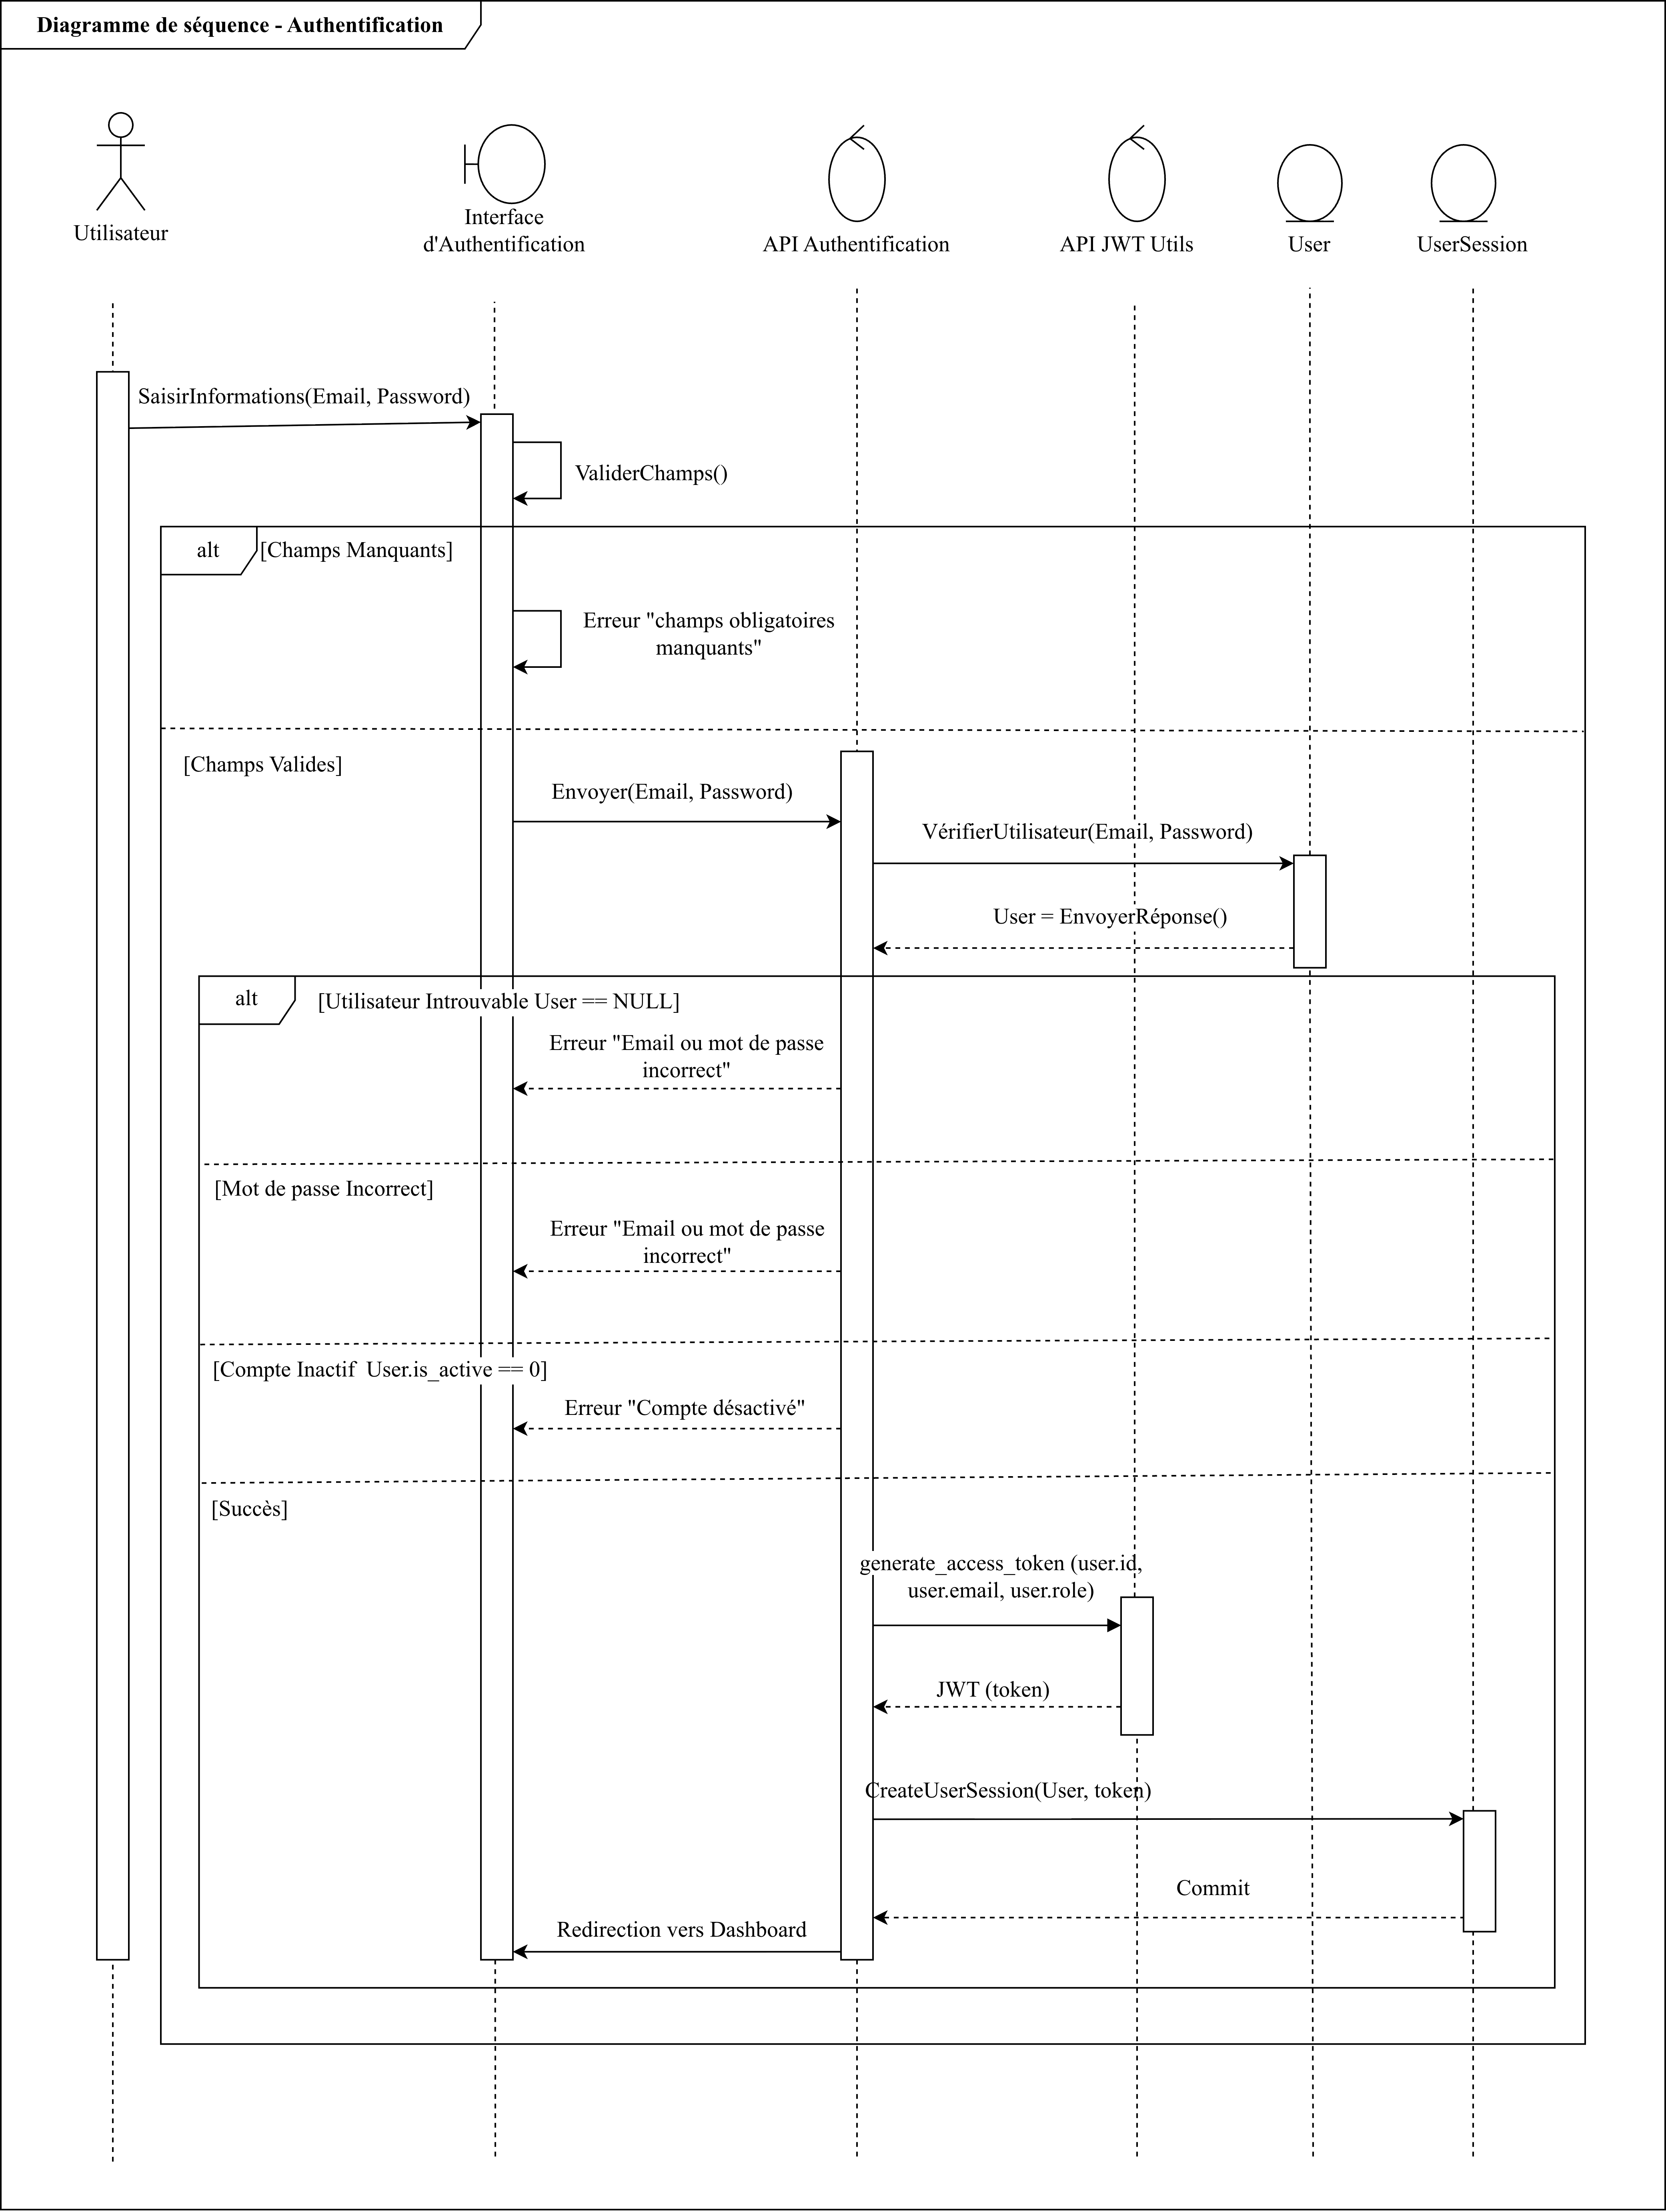
\includegraphics[width=0.92\linewidth]{figures/chapitre-03/diagramme-sequence-s-authentifier.png}
  \caption{Diagramme de séquence — «~S’authentifier~».}
  \label{fig:doc-ch3-seq-auth}
\end{figure}%
}{%
\begin{figure}[H]
  \centering
  \fbox{\parbox{0.92\linewidth}{\centering\vspace{3.2cm}\textit{(Figure à insérer : \texttt{figures/chapitre-03/diagramme-sequence-s-authentifier.png})}\vspace{3.2cm}}}
  \caption{Diagramme de séquence — «~S’authentifier~».}
  \label{fig:doc-ch3-seq-auth}
\end{figure}%
}

\subsubsection{Diagramme de séquence : «~Créer un site~»}

La figure~\ref{fig:doc-ch3-seq-site} présente le diagramme de séquence du cas d’utilisation «~Créer un site~».

\IfFileExists{figures/chapitre-03/diagramme-sequence-creer-un-site.png}{%
\begin{figure}[H]
  \centering
  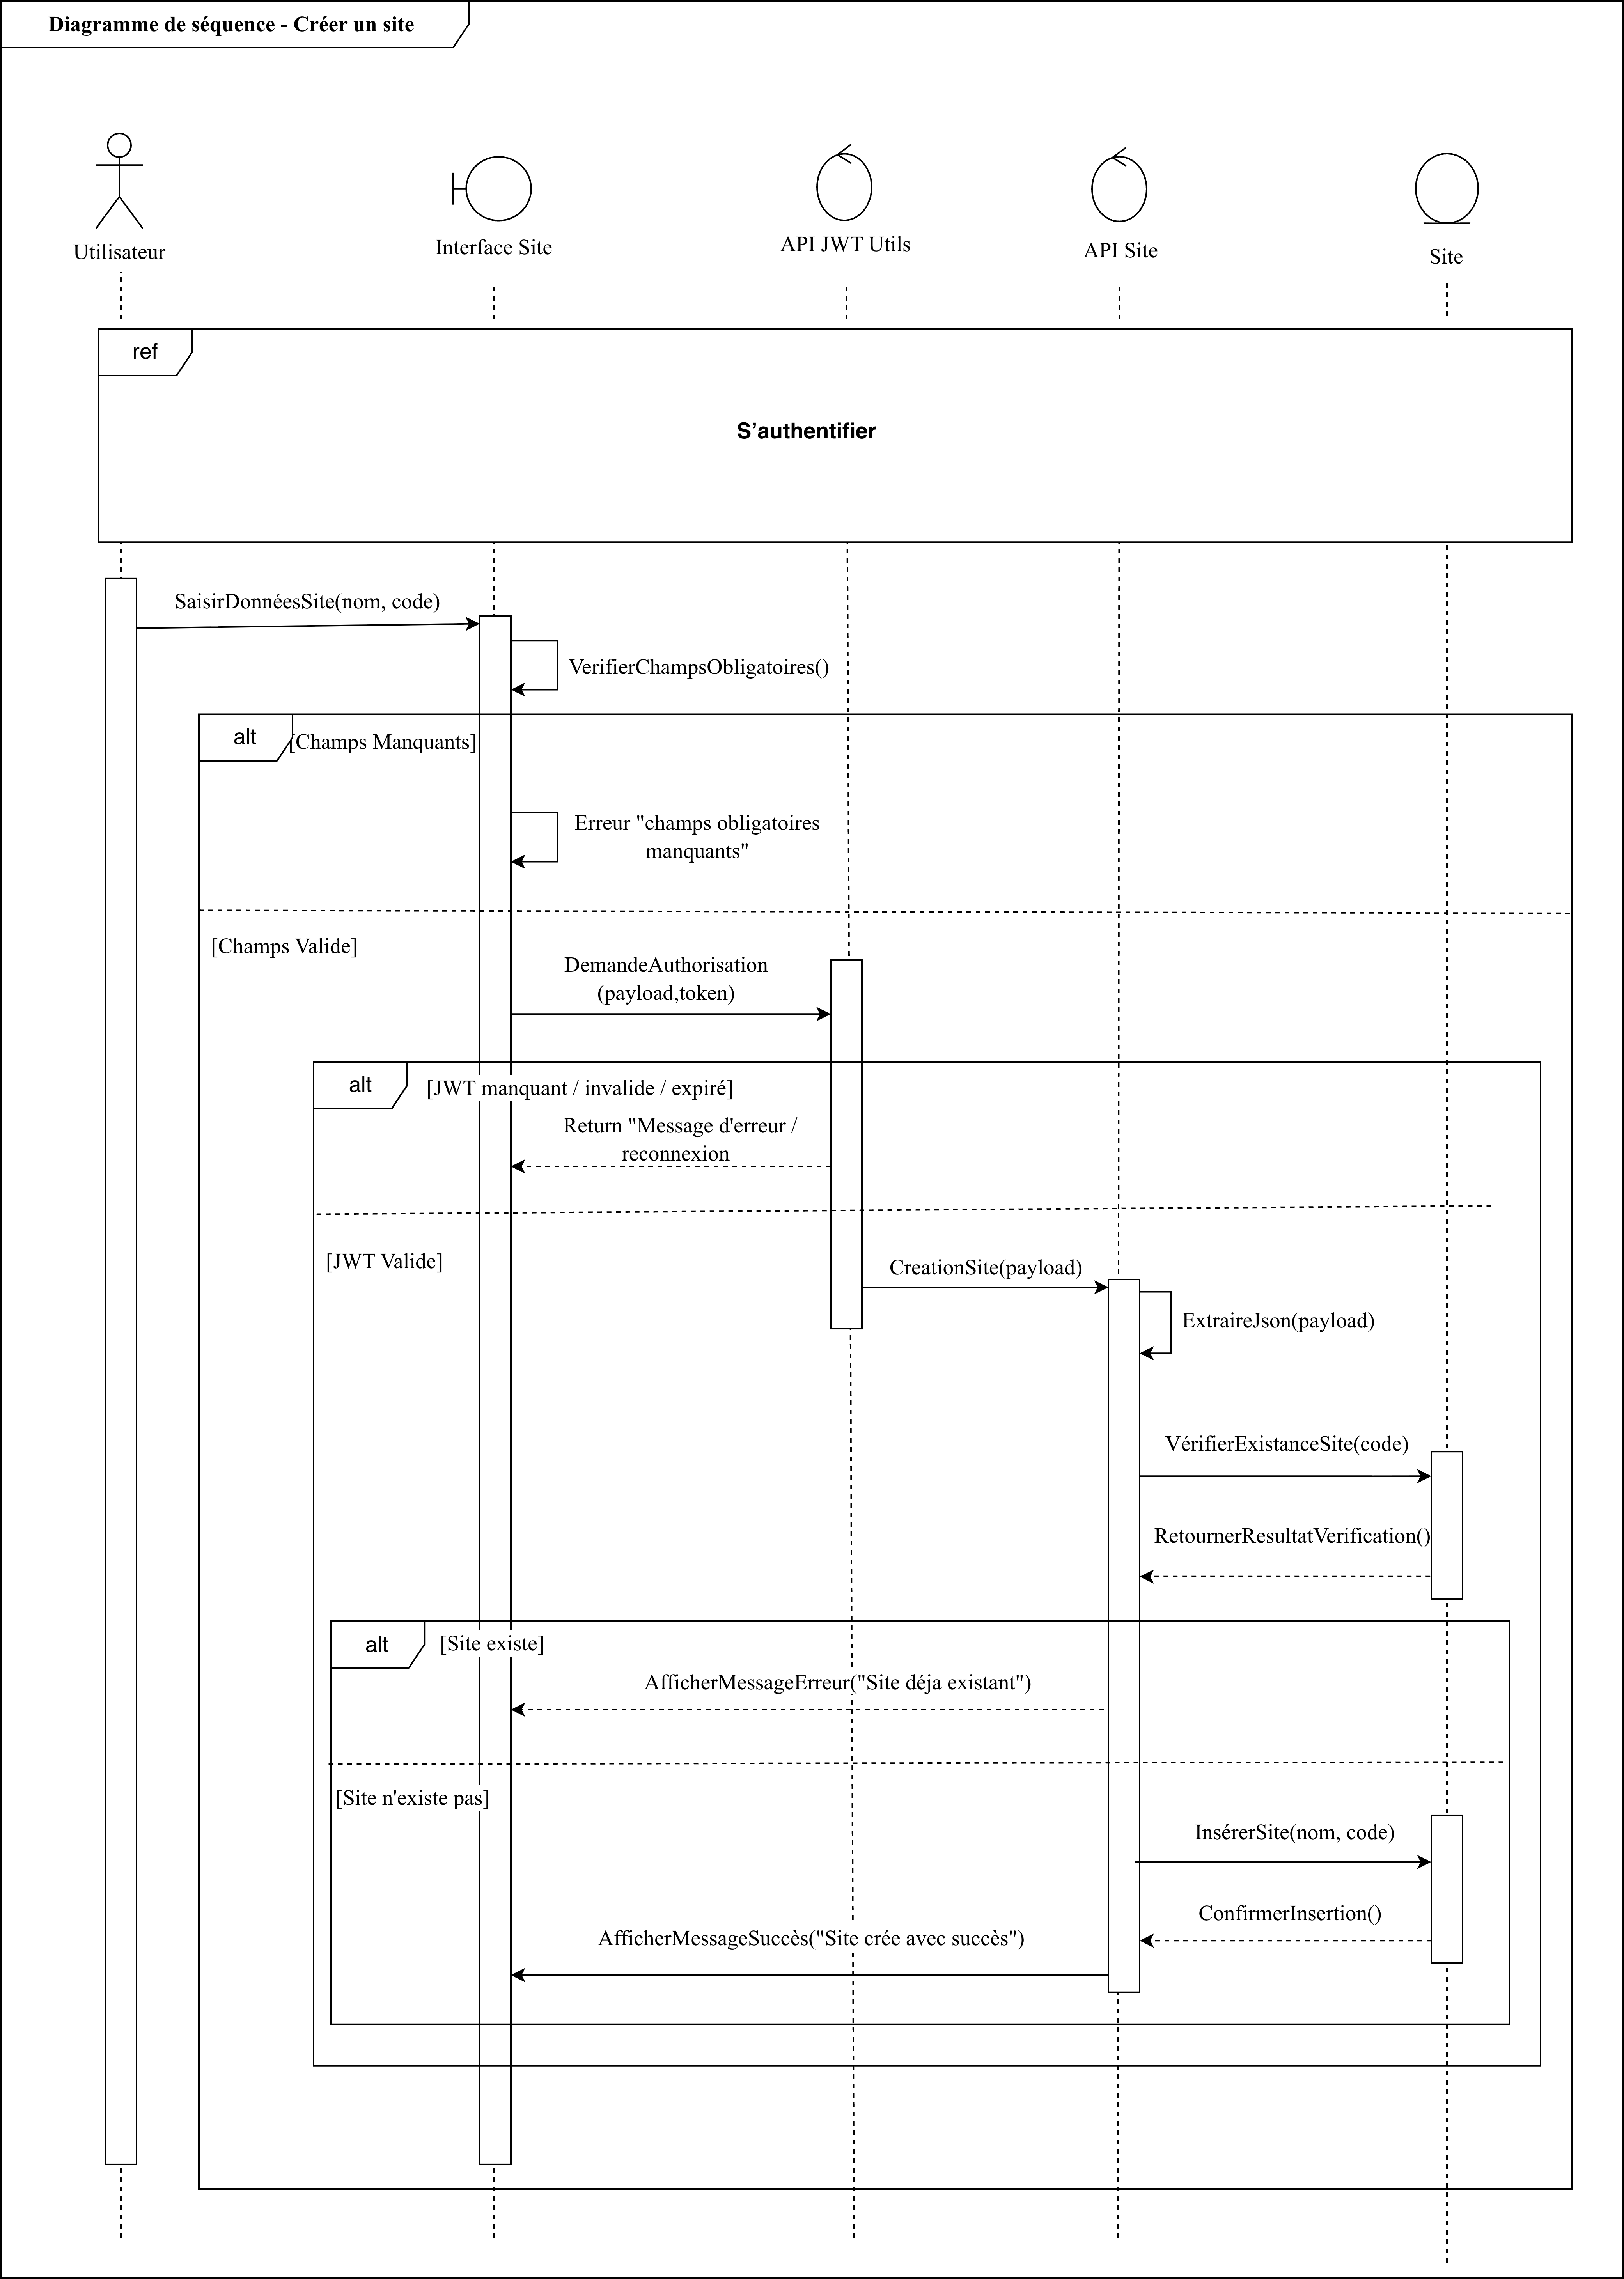
\includegraphics[width=0.92\linewidth]{figures/chapitre-03/diagramme-sequence-creer-un-site.png}
  \caption{Diagramme de séquence — «~Créer un site~».}
  \label{fig:doc-ch3-seq-site}
\end{figure}%
}{%
\begin{figure}[H]
  \centering
  \fbox{\parbox{0.92\linewidth}{\centering\vspace{3.2cm}\textit{(Figure à insérer : \texttt{figures/chapitre-03/diagramme-sequence-creer-un-site.png})}\vspace{3.2cm}}}
  \caption{Diagramme de séquence — «~Créer un site~».}
  \label{fig:doc-ch3-seq-site}
\end{figure}%
}

\subsubsection{Diagramme de séquence : «~Créer un utilisateur~»}

La figure~\ref{fig:doc-ch3-seq-user} présente le diagramme de séquence du cas d’utilisation «~Créer un utilisateur~».

\IfFileExists{figures/chapitre-03/diagramme-sequence-creer-un-utilisateur.png}{%
\begin{figure}[H]
  \centering
  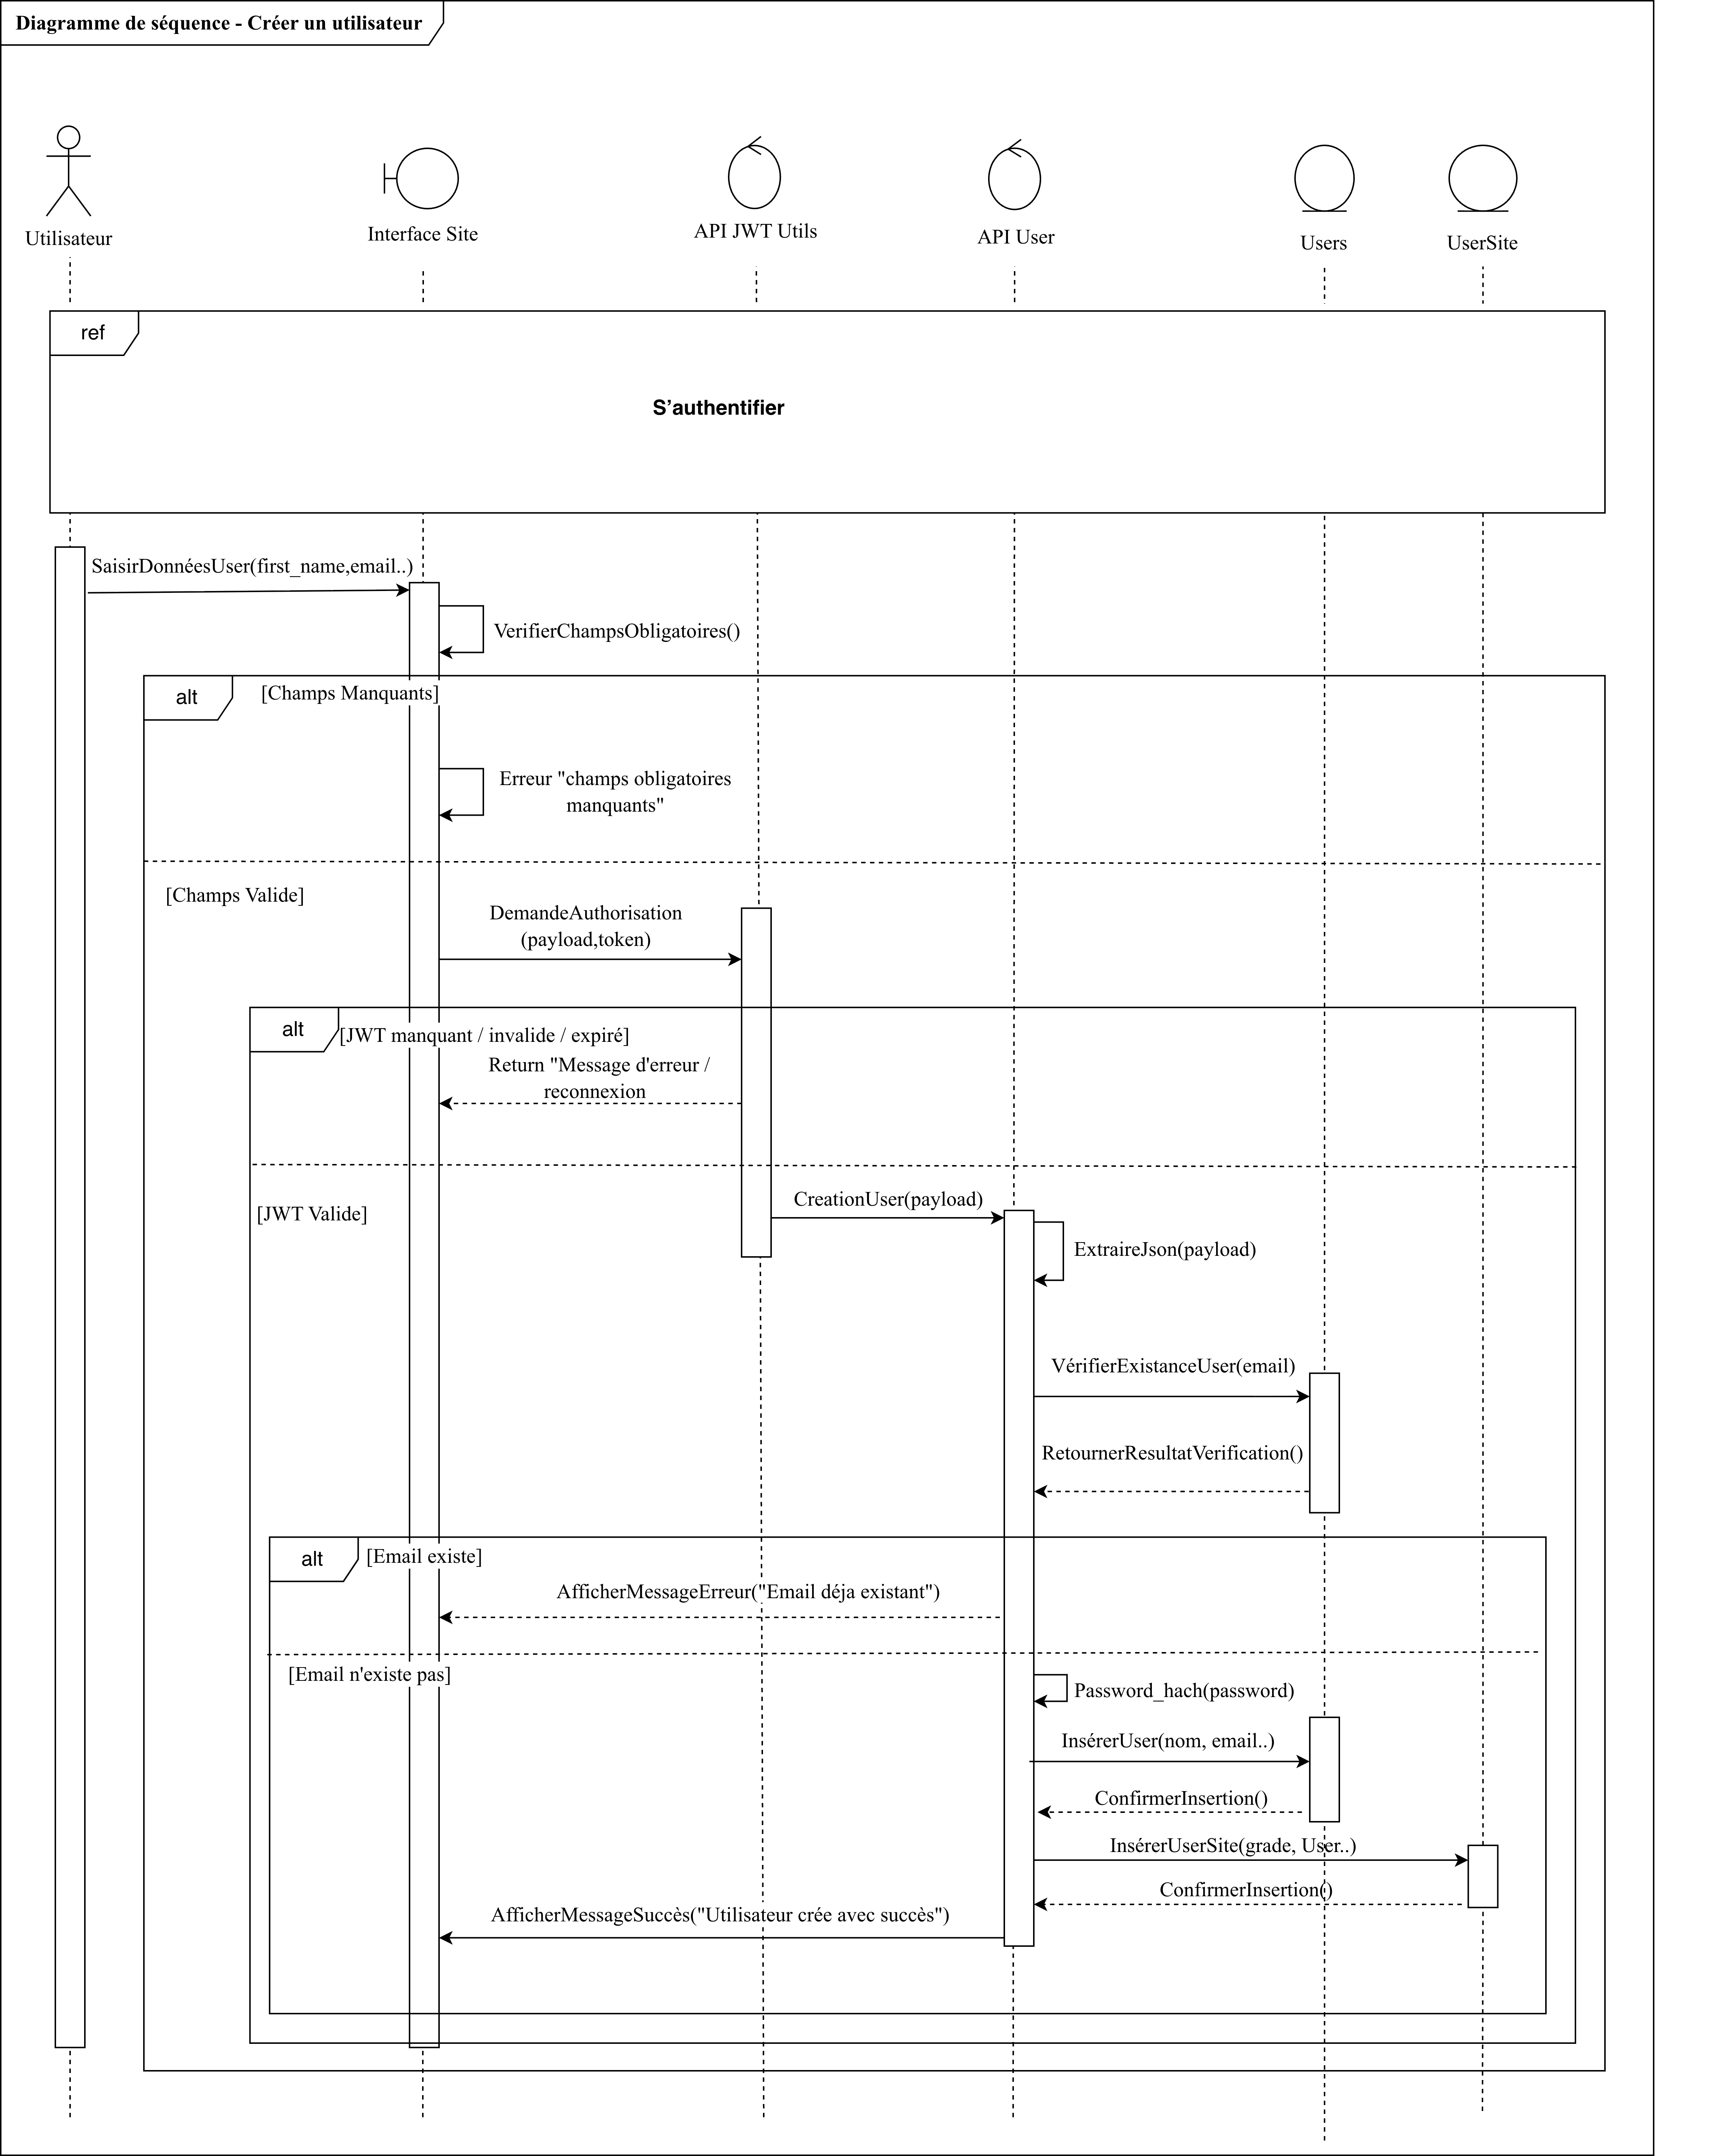
\includegraphics[width=1\linewidth]{figures/chapitre-03/diagramme-sequence-creer-un-utilisateur.png}
  \caption{Diagramme de séquence — «~Créer un utilisateur~».}
  \label{fig:doc-ch3-seq-user}
\end{figure}%
}{%
\begin{figure}[H]
  \centering
  \fbox{\parbox{1\linewidth}{\centering\vspace{3.2cm}\textit{(Figure à insérer : \texttt{figures/chapitre-03/diagramme-sequence-creer-un-utilisateur.png})}\vspace{3.2cm}}}
  \caption{Diagramme de séquence — «~Créer un utilisateur~».}
  \label{fig:doc-ch3-seq-user}
\end{figure}%
}

\subsection{Diagramme d’activité}

Les diagrammes d’activité illustrent le déroulement des traitements métier et les décisions principales pour les cas d'utilisation du sprint 1.

\subsubsection{Diagramme d’activité : «~S’authentifier~»}

La figure~\ref{fig:doc-ch3-act-auth} présente le diagramme d’activité du cas d’utilisation «~S’authentifier~».

\IfFileExists{figures/chapitre-03/Diagramme_dactivite_Sauthentifier.png}{%
\begin{figure}[H]
  \centering
  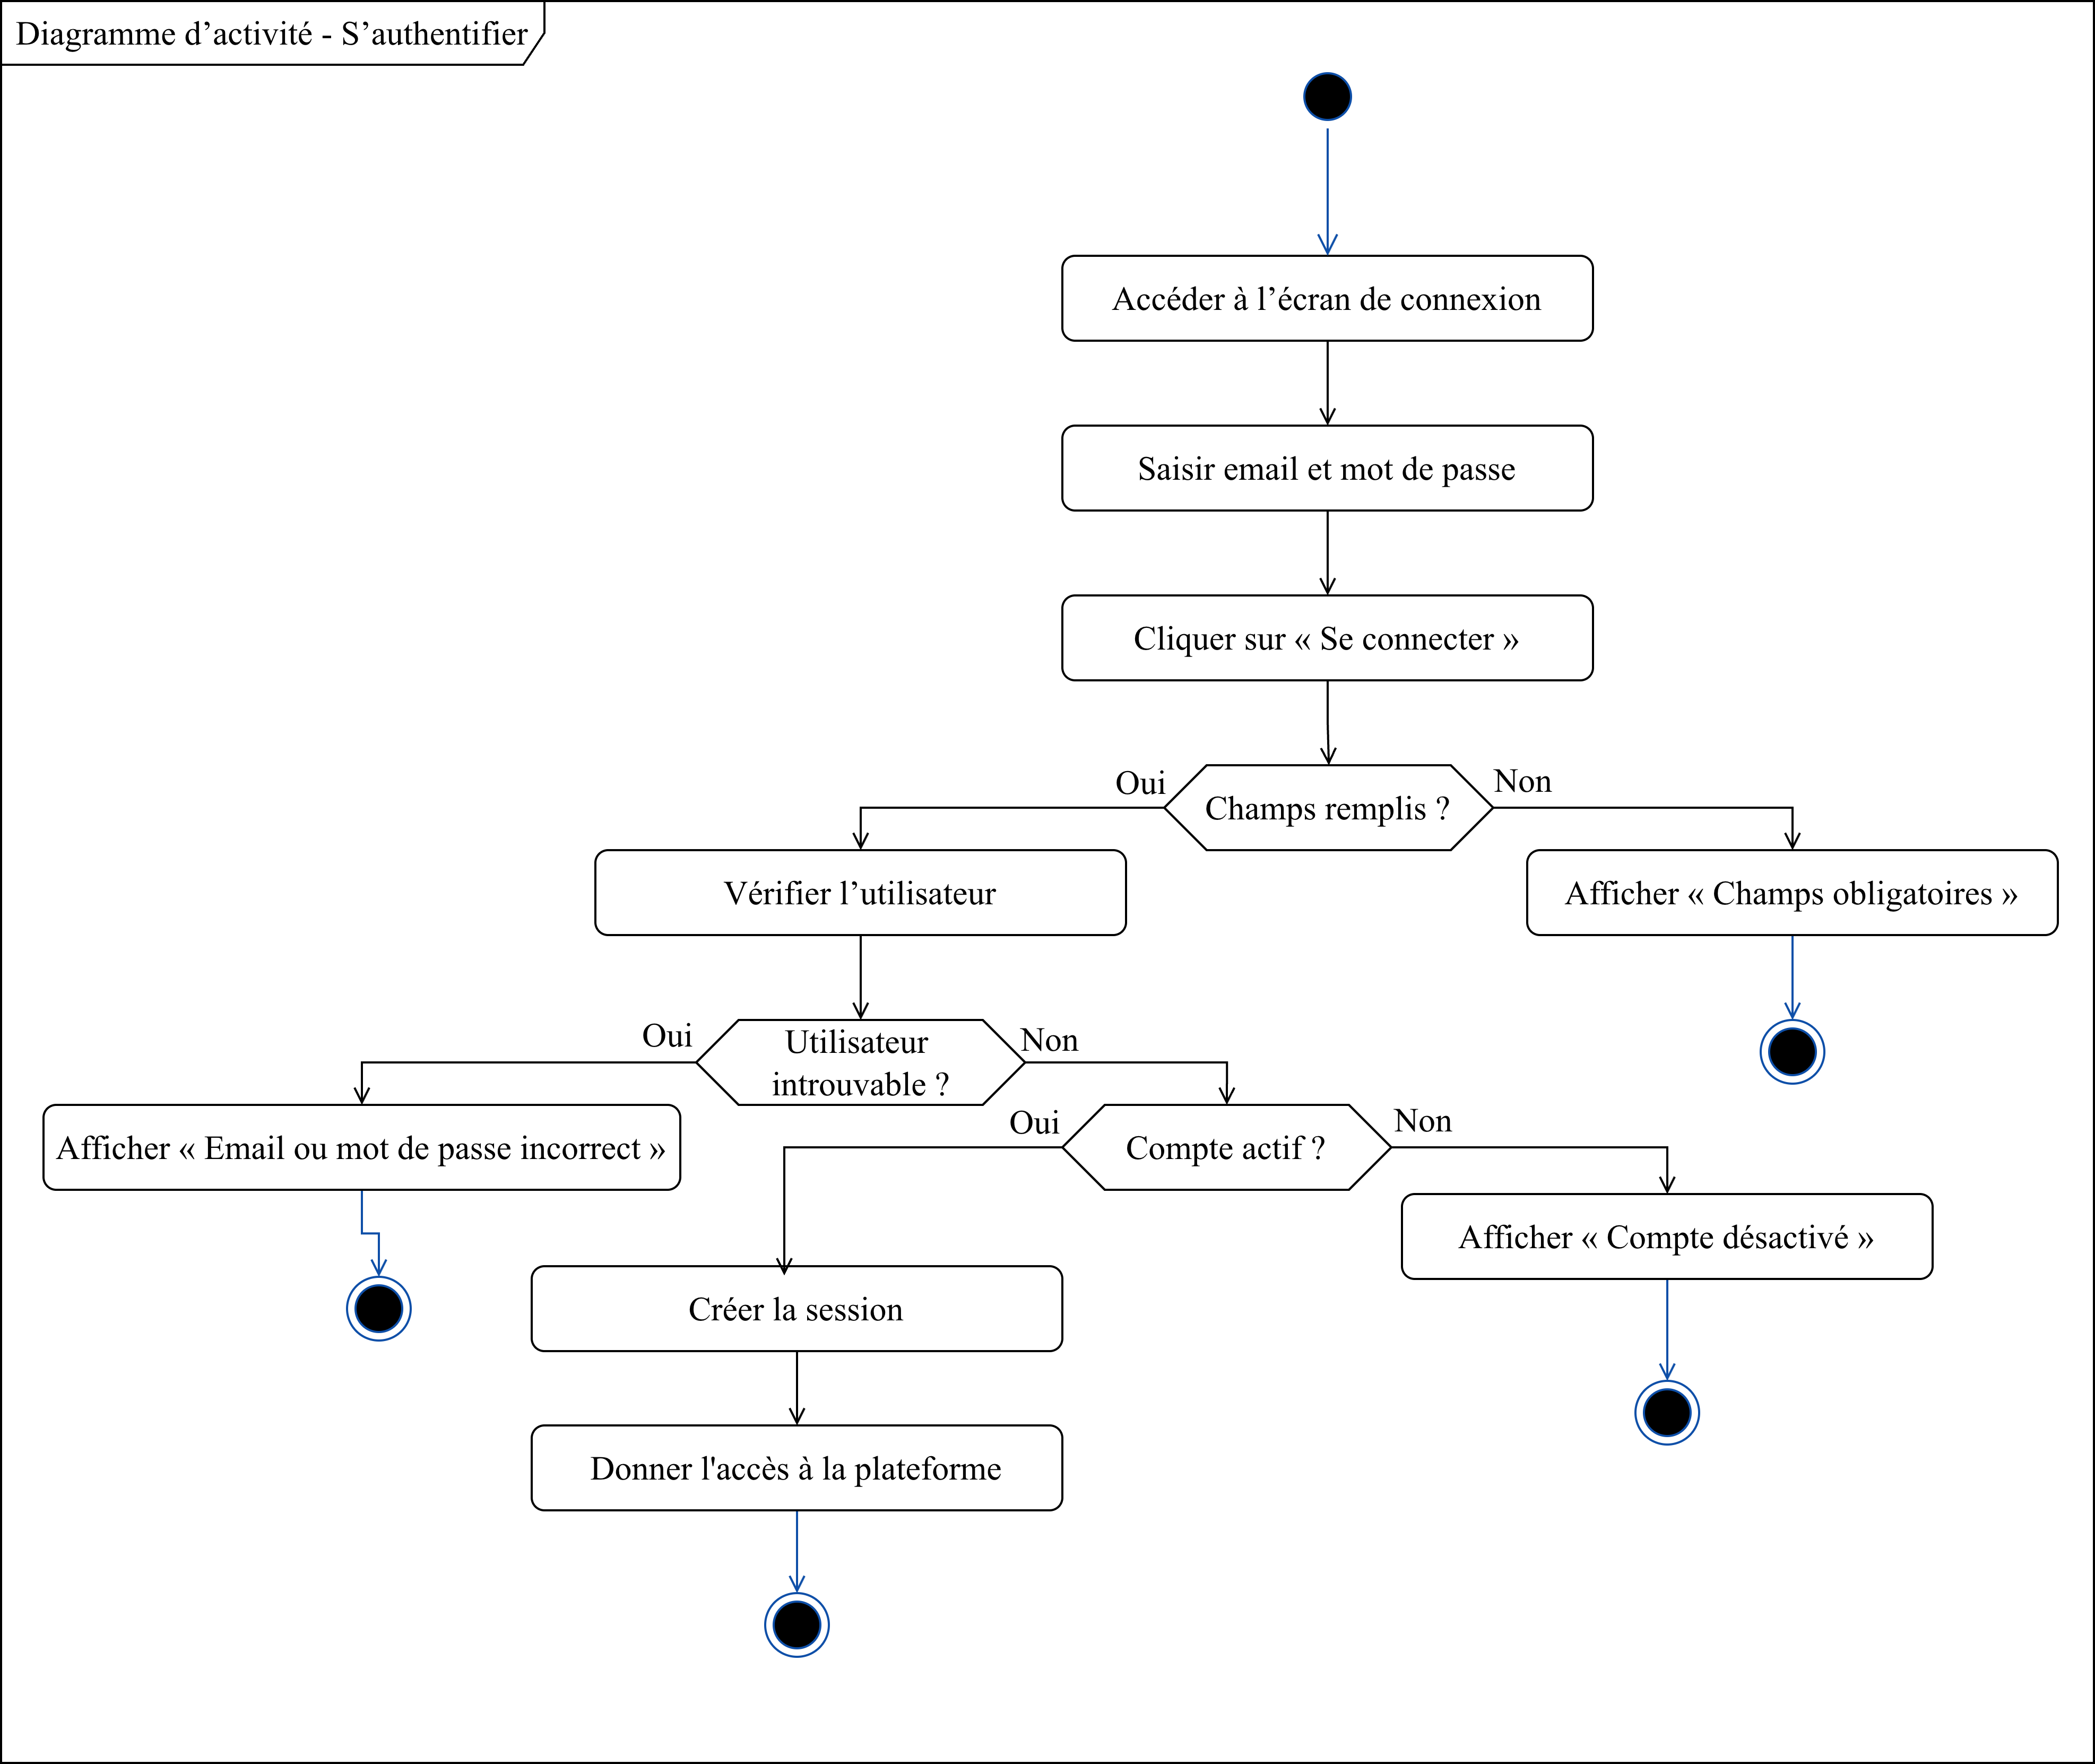
\includegraphics[width=0.92\linewidth]{figures/chapitre-03/Diagramme_dactivite_Sauthentifier.png}
  \caption{Diagramme d’activité — «~S’authentifier~».}
  \label{fig:doc-ch3-act-auth}
\end{figure}%
}{%
\begin{figure}[H]
  \centering
  \fbox{\parbox{0.92\linewidth}{\centering\vspace{3.2cm}\textit{(Figure à insérer : \texttt{figures/chapitre-03/Diagramme\_dactivite\_Sauthentifier.png})}\vspace{3.2cm}}}
  \caption{Diagramme d’activité — «~S’authentifier~».}
  \label{fig:doc-ch3-act-auth}
\end{figure}%
}

\subsubsection{Diagramme d’activité : «~Créer un site~»}

La figure~\ref{fig:doc-ch3-act-site} présente le diagramme d’activité du cas d’utilisation «~Créer un site~».

\IfFileExists{figures/chapitre-03/Diagramme_dactivite_cree_un_site.png}{%
\begin{figure}[H]
  \centering
  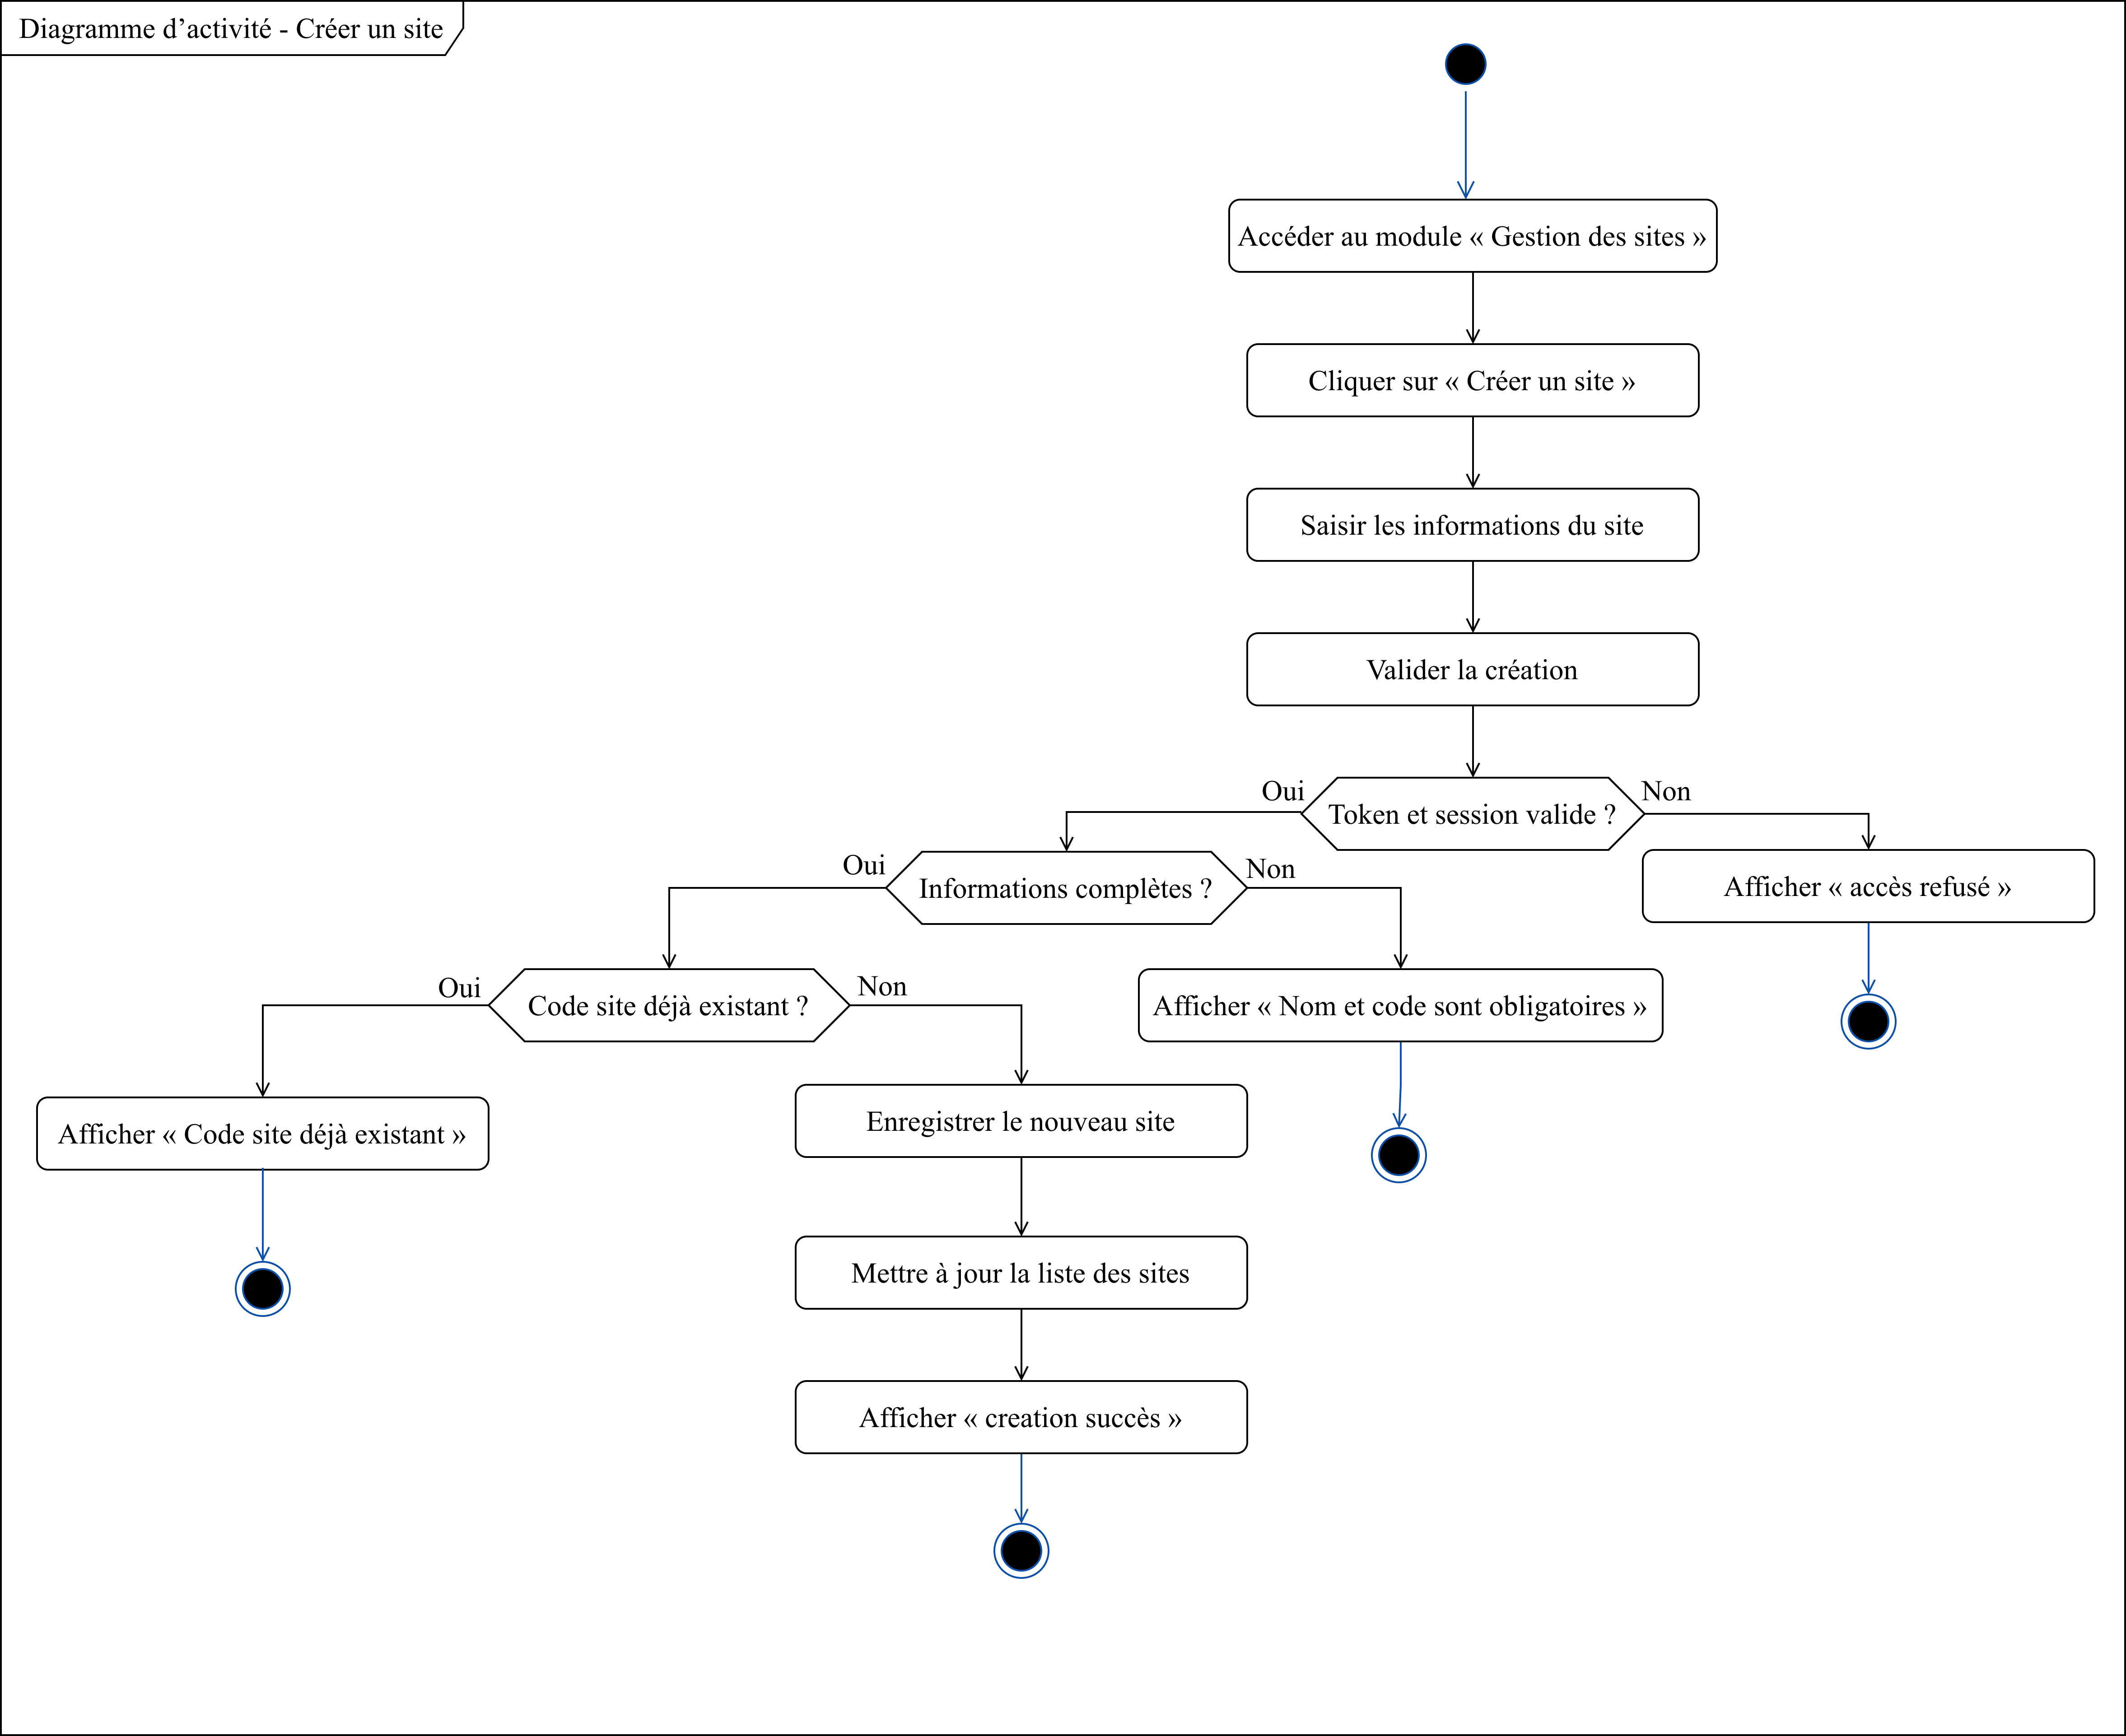
\includegraphics[width=0.92\linewidth]{figures/chapitre-03/Diagramme_dactivite_cree_un_site.png}
  \caption{Diagramme d’activité — «~Créer un site~».}
  \label{fig:doc-ch3-act-site}
\end{figure}%
}{%
\begin{figure}[H]
  \centering
  \fbox{\parbox{0.92\linewidth}{\centering\vspace{3.2cm}\textit{(Figure à insérer : \texttt{figures/chapitre-03/Diagramme\_dactivite\_cree\_un\_site.png})}\vspace{3.2cm}}}
  \caption{Diagramme d’activité — «~Créer un site~».}
  \label{fig:doc-ch3-act-site}
\end{figure}%
}

\subsubsection{Diagramme d’activité : «~Créer un utilisateur~»}

La figure~\ref{fig:doc-ch3-act-user} présente le diagramme d’activité du cas d’utilisation «~Créer un utilisateur~».

\IfFileExists{figures/chapitre-03/Diagramme_dactivite_cree_un_utilisateur.png}{%
\begin{figure}[H]
  \centering
  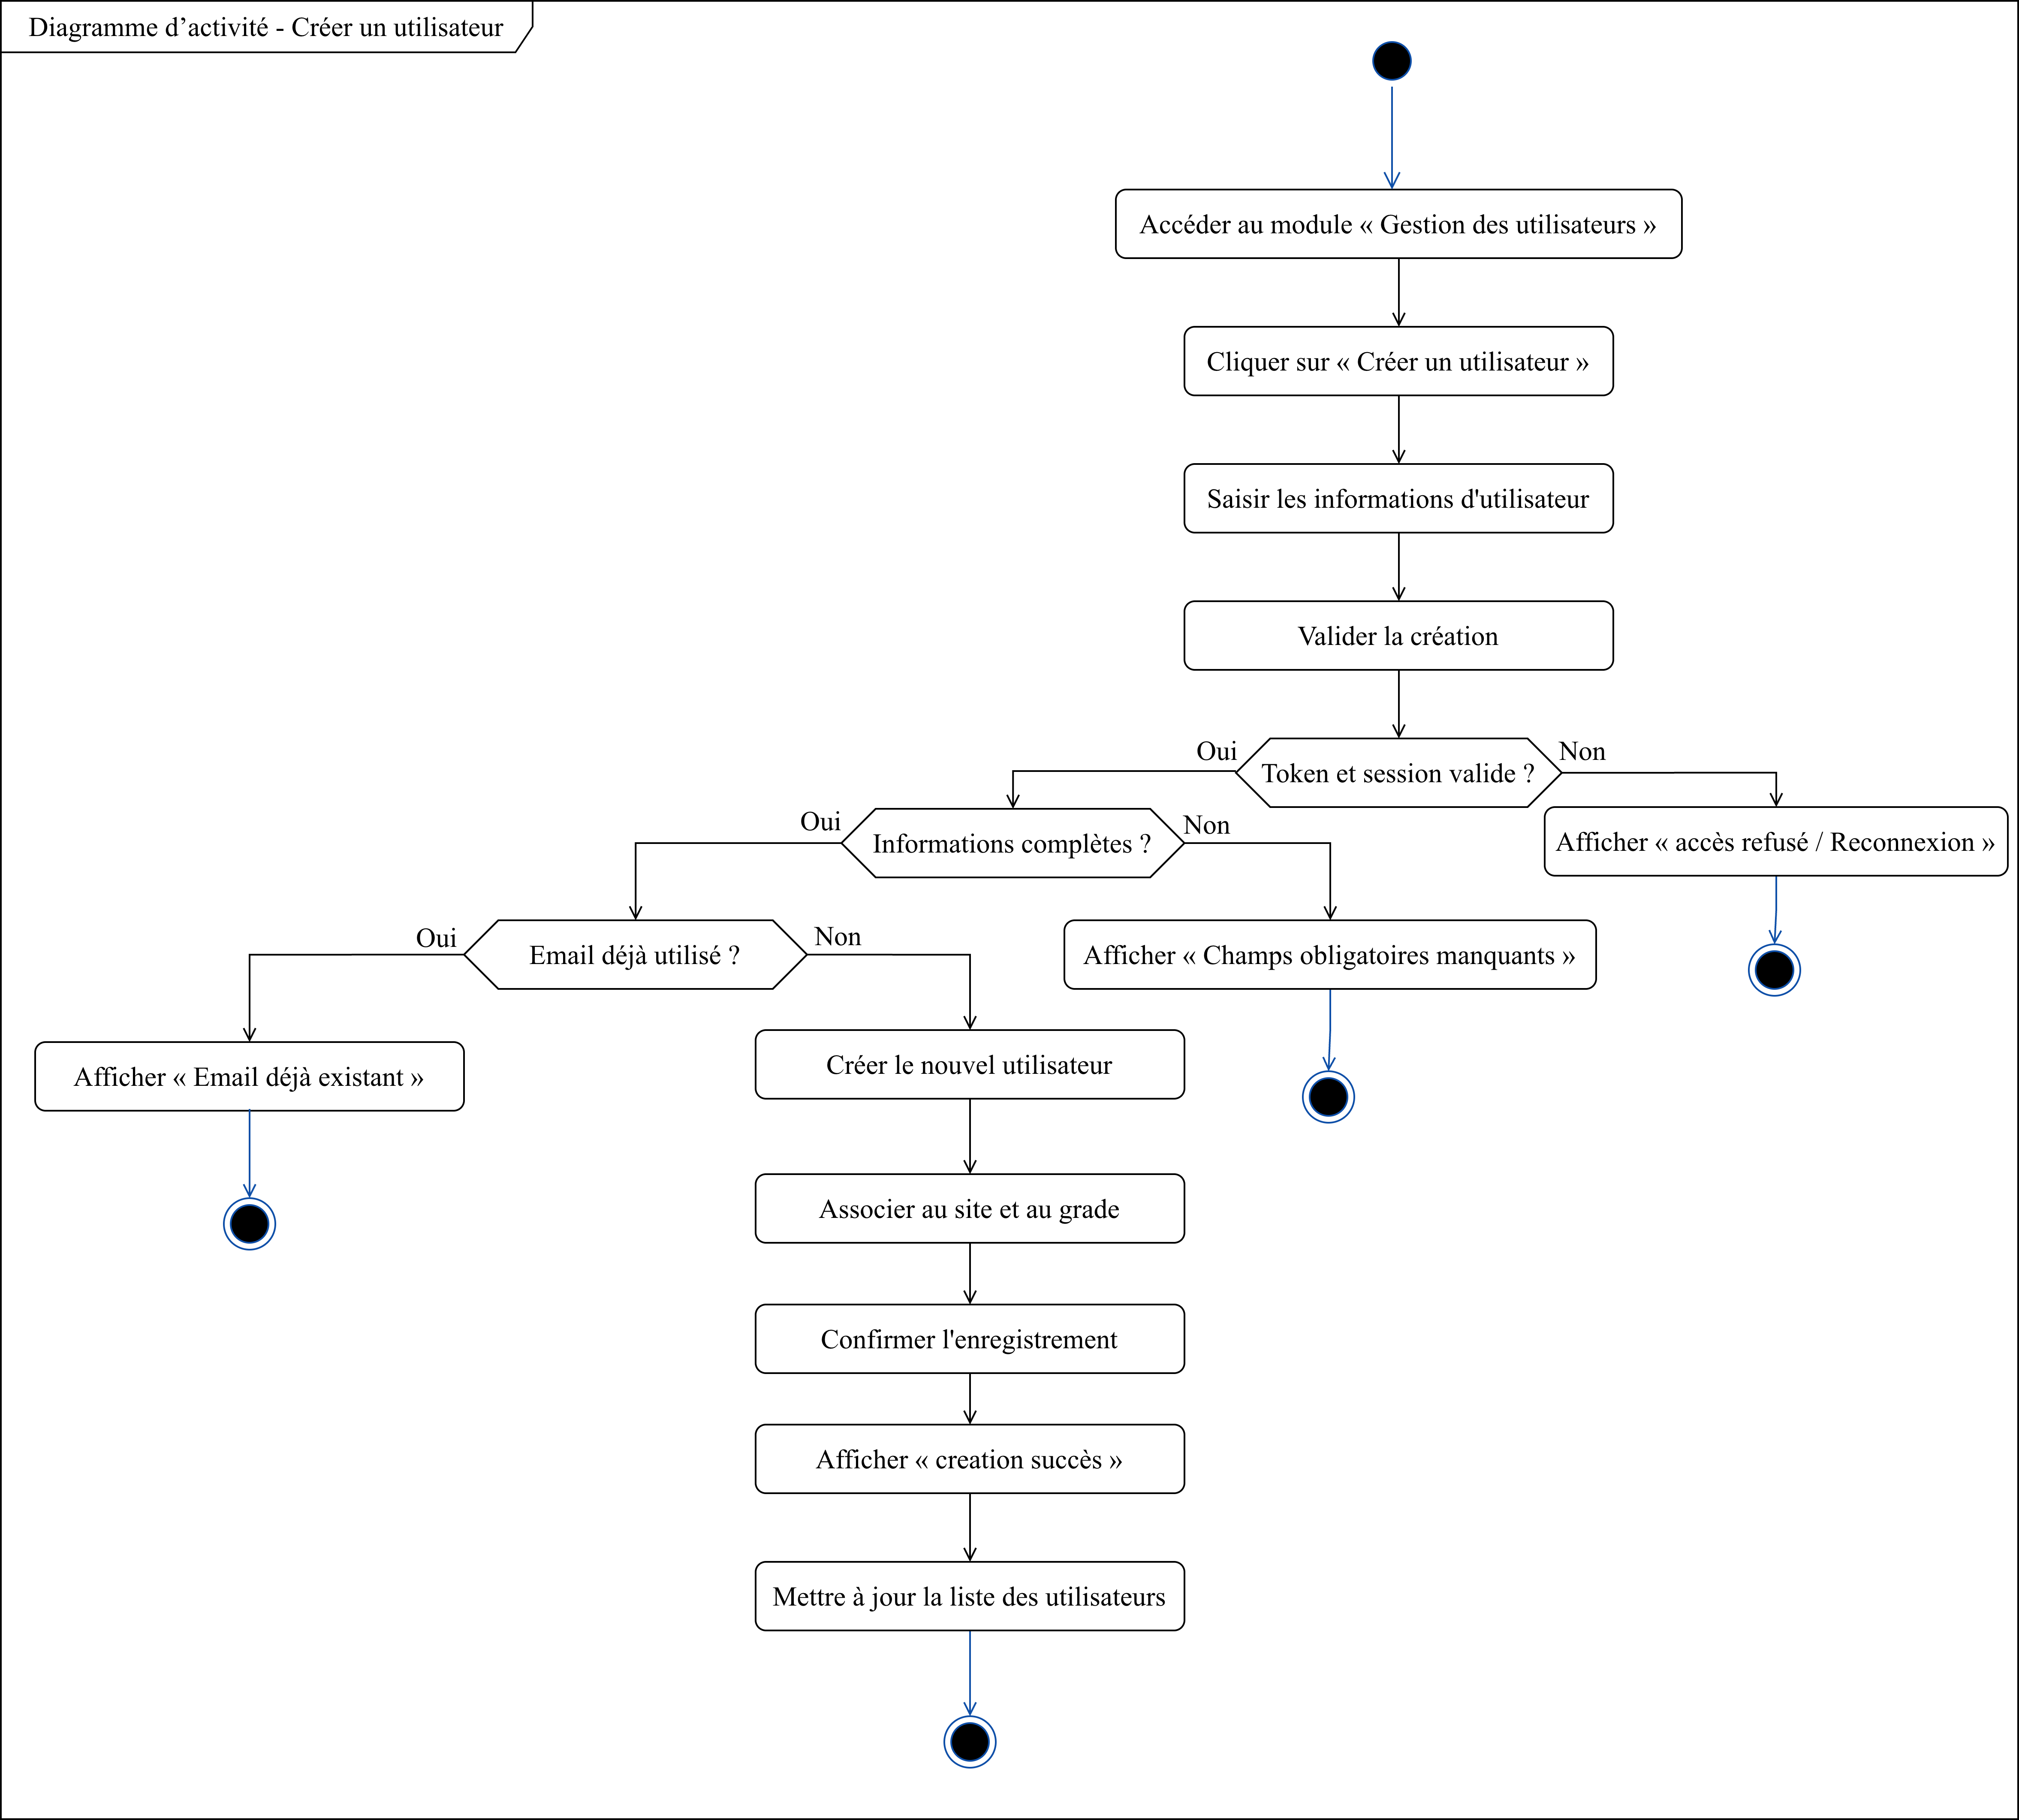
\includegraphics[width=0.92\linewidth]{figures/chapitre-03/Diagramme_dactivite_cree_un_utilisateur.png}
  \caption{Diagramme d’activité — «~Créer un utilisateur~».}
  \label{fig:doc-ch3-act-user}
\end{figure}%
}{%
\begin{figure}[H]
  \centering
  \fbox{\parbox{0.92\linewidth}{\centering\vspace{3.2cm}\textit{(Figure à insérer : \texttt{figures/chapitre-03/Diagramme\_dactivite\_cree\_un\_utilisateur.png})}\vspace{3.2cm}}}
  \caption{Diagramme d’activité — «~Créer un utilisateur~».}
  \label{fig:doc-ch3-act-user}
\end{figure}%
}

\section{Réalisation}

Dans cette section, nous illustrons le travail réalisé durant ce sprint à travers un ensemble de captures d’écran de la plateforme. Ces visuels permettent de mettre en évidence les principales fonctionnalités développées et d'avoir une vision concrète du résultat obtenu.

La figure~\ref{fig:doc-ch3-3} présente l’interface de la liste des utilisateurs.

\begin{figure}[H]
  \centering
  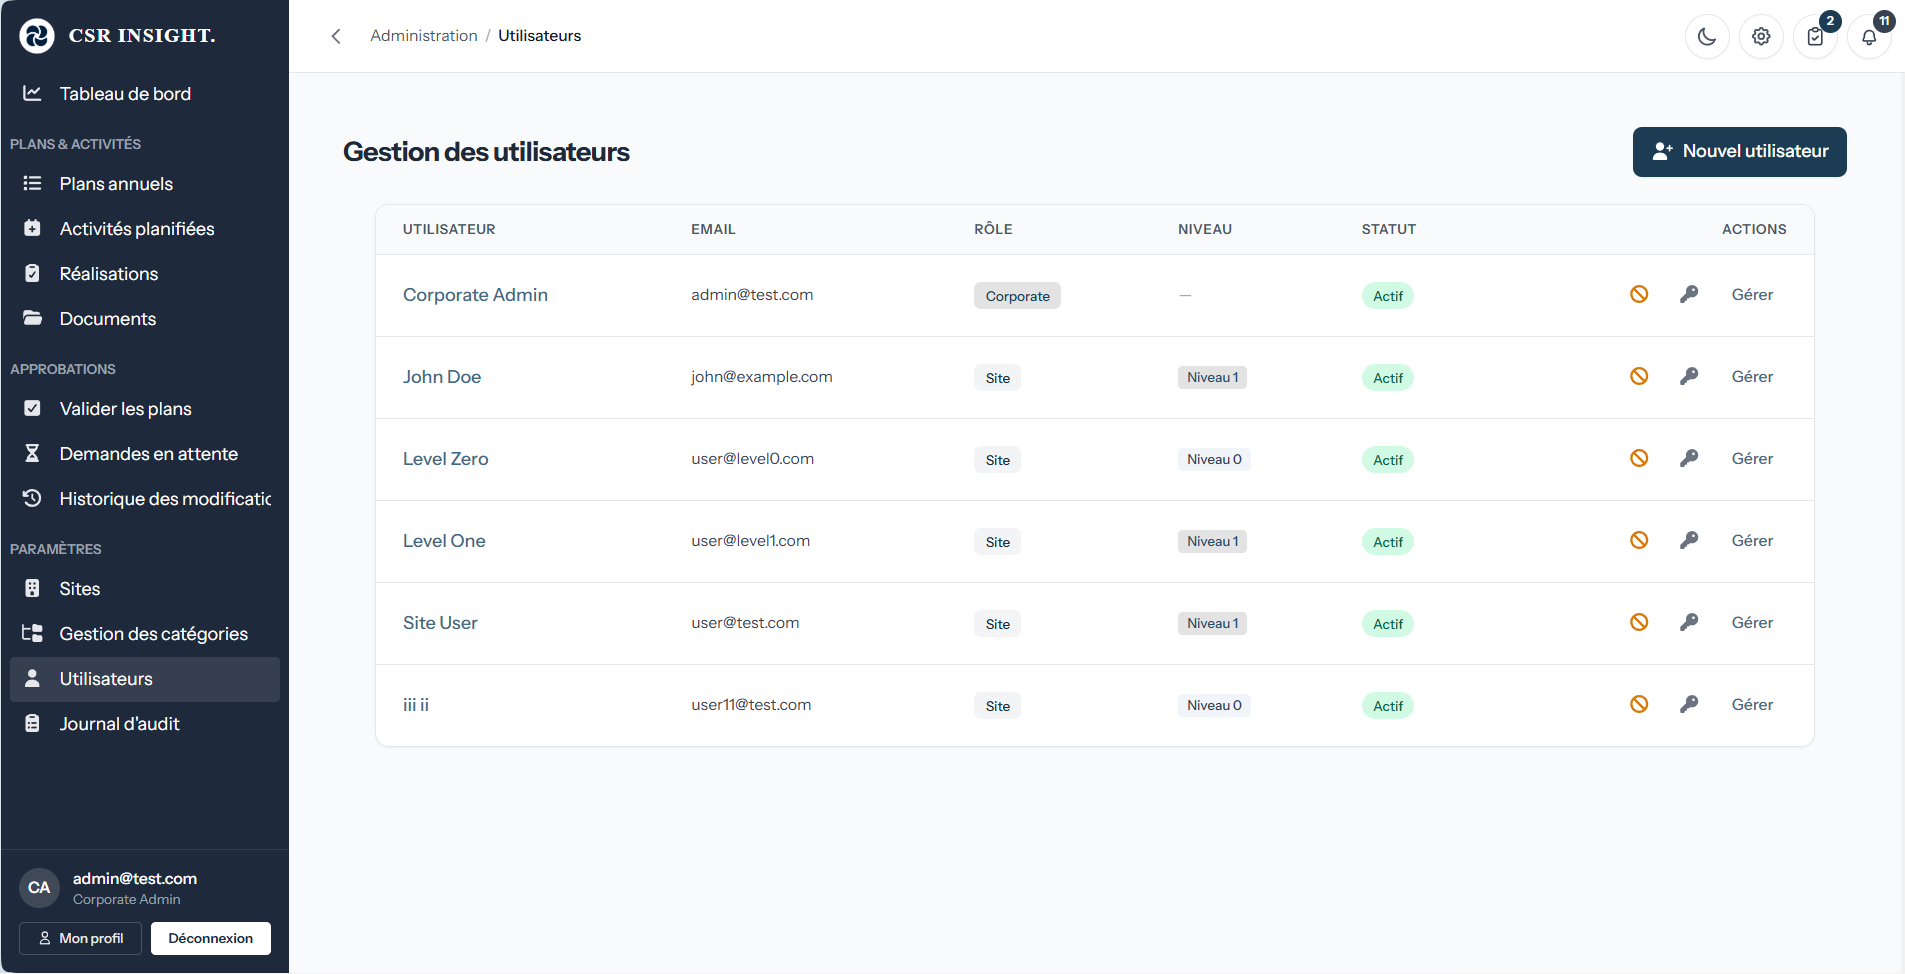
\includegraphics[width=0.92\linewidth]{figures/chapitre-03/ui-gestion-utilisateurs.png}
  \caption{Interface - gestion des utilisateurs.}
  \label{fig:doc-ch3-3}
\end{figure}

Cette interface présente la page de gestion des utilisateurs de la plateforme. Elle permet à l’utilisateur Corporate de consulter les comptes enregistrés via un tableau affichant le nom, le rôle, le niveau d’approbation et le statut. Elle offre également des fonctionnalités de gestion telles que l’ajout, la modification et la désactivation des utilisateurs.

La figure~\ref{fig:doc-ch3-4} présente l’interface de la liste des sites.
\newpage
\begin{figure}[H]
  \centering
  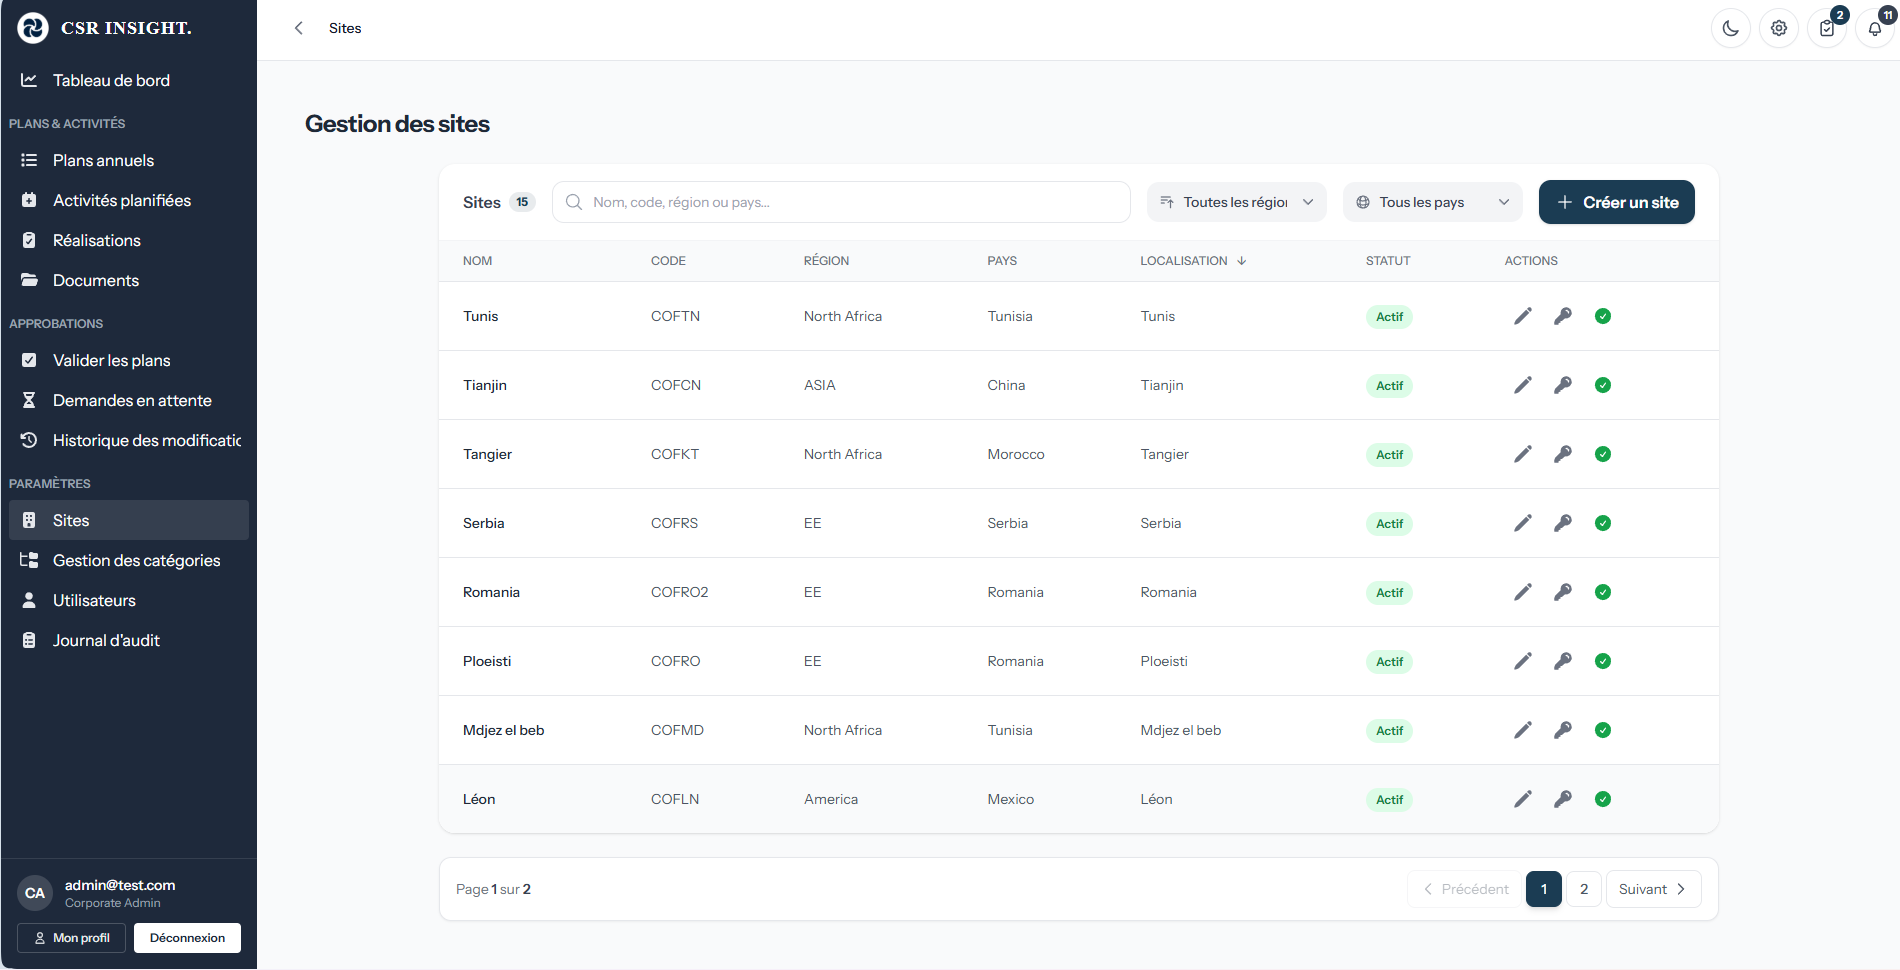
\includegraphics[width=0.92\linewidth]{figures/chapitre-03/ui-gestion-sites.png}
  \caption{Interface - gestion des sites.}
  \label{fig:doc-ch3-4}
\end{figure}

Cette interface présente la page Gestion des sites de la plateforme, dédiée à l’administration et à la configuration des différents sites opérationnels de Coficab à l’échelle internationale. Elle offre une vue centralisée sous forme de tableau listant les sites avec leurs informations essentielles, notamment le nom, le code, la région, le pays, ainsi que leur localisation géographique et leur statut d’activation.

La page intègre des fonctionnalités avancées de recherche et de filtrage permettant d’affiner l’affichage des sites selon plusieurs critères tels que la région ou le pays, facilitant ainsi l’analyse et la gestion dans un contexte multi-sites. L’utilisateur Corporate peut également créer un nouveau site via un bouton dédié, ou effectuer des actions spécifiques sur chaque entrée (modification, activation ou ajouter des utilisateurs à un site bien précis ).


La figure~\ref{fig:doc-ch3-6} présente l’interface de gestion des documents.

\IfFileExists{figures/chapitre-03/ui-gestion-documents.png}{%
\begin{figure}[H]
  \centering
  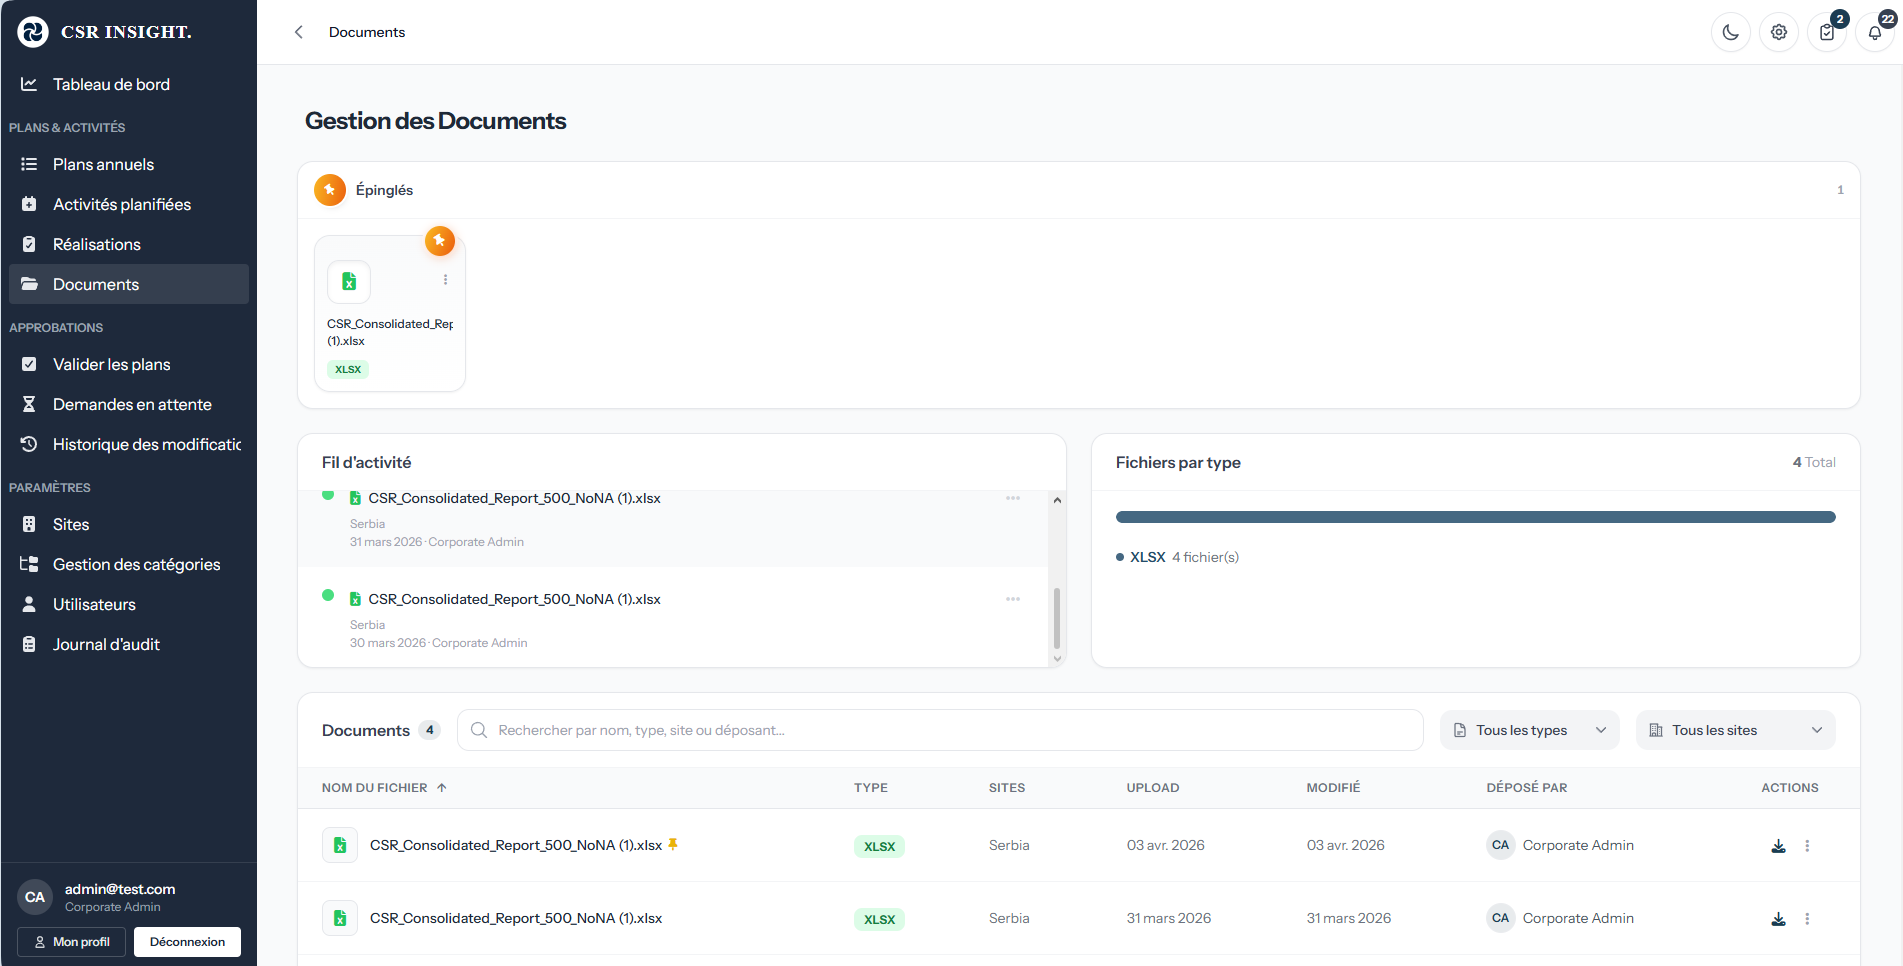
\includegraphics[width=0.92\linewidth]{figures/chapitre-03/ui-gestion-documents.png}
  \caption{Interface : gestion des documents.}
  \label{fig:doc-ch3-6}
\end{figure}%
}{%
\begin{figure}[H]
  \centering
  \fbox{\parbox{0.92\linewidth}{\centering\vspace{3.2cm}\textit{(Figure à insérer : \texttt{figures/chapitre-03/ui-gestion-documents.png})}\vspace{3.2cm}}}
  \caption{Interface : gestion des documents.}
  \label{fig:doc-ch3-6}
\end{figure}%
}

\section{Tests et validation}

Les tests jouent un rôle essentiel dans la méthodologie agile~: ils contribuent à la qualité et à la fiabilité des fonctionnalités livrées. Avant d’enclencher un nouveau sprint, il est nécessaire de vérifier les incréments prioritaires afin de s’assurer du bon fonctionnement et de l’adéquation avec les besoins des acteurs.

\subsection{Test}

Dans cette partie, nous présentons une validation fonctionnelle synthétique des principales fonctionnalités du premier sprint «~Authentification \& Architecture de base~», en couvrant l'\textbf{authentification}, la \textbf{gestion des utilisateurs} et la \textbf{gestion des sites} à travers un tableau consolidé de cas de test.




Le tableau~\ref{tab:ch3-scenarios-tests} présente une synthèse consolidée des cas de test du sprint 1.
% Scénarios de test consolidés — chapitre 3 (authentification, utilisateurs, sites)
\small
\PFETableSetup
\setlength{\LTpre}{0pt}
\setlength{\LTpost}{0pt}
\setlength{\LTleft}{-0.8cm}
\setlength{\LTright}{-0.8cm}
\renewcommand{\arraystretch}{1.25}

\begin{longtable}{|>{\centering\arraybackslash}m{3.1cm}|
>{\raggedright\arraybackslash}p{2.9cm}|
>{\raggedright\arraybackslash}p{4.4cm}|
>{\raggedright\arraybackslash}p{5.0cm}|
>{\centering\arraybackslash}p{1.3cm}|}
\caption{Synthèse des cas de test — Authentification \& Architecture de base}\label{tab:ch3-scenarios-tests}\\
\hline
\tableHeaderStyle
\tableHeaderCell{Nom du cas d'utilisation} &
\tableHeaderCell{Cas de test} &
\tableHeaderCell{Description du cas} &
\tableHeaderCell{Résultat attendu} &
\tableHeaderCell{Résultat réel} \\
\hline
\endfirsthead
\hline
\multicolumn{5}{|c|}{\tablename\ \thetable{} --- \textit{(suite)}} \\
\hline
\tableHeaderStyle
\tableHeaderCell{Nom du cas d'utilisation} &
\tableHeaderCell{Cas de test} &
\tableHeaderCell{Description du cas} &
\tableHeaderCell{Résultat attendu} &
\tableHeaderCell{Résultat réel} \\
\hline
\endhead
\hline
\multicolumn{5}{|r|}{\textit{Suite page suivante\ldots}} \\
\hline
\endfoot
\hline
\endlastfoot

\multirow{2}{=}{\centering S'authentifier} &
Identifiants manquants &
Tentative de connexion sans renseigner l'email ou le mot de passe. &
Message indiquant que les champs d'authentification sont obligatoires. &
Vrai \\
\cline{2-5}

 &
Identifiants invalides &
Tentative de connexion avec des informations incorrectes. &
Message d'échec d'authentification. &
Vrai \\
\hline

Accéder à Dashboard &
Utilisateur non authentifié &
L'utilisateur tente d'accéder au tableau de bord sans session valide. &
Redirection vers la page de connexion ou message d'accès refusé. &
Vrai \\
\hline

\multirow{5}{=}{\centering Gérer \\les utilisateurs} &
Afficher la liste des utilisateurs &
Ouverture du module de gestion des utilisateurs par un profil autorisé. &
La liste des utilisateurs s'affiche correctement. &
Vrai \\
\cline{2-5}

 &
Créer un utilisateur &
Création d'un nouveau compte avec des informations valides. &
Le compte est créé et apparaît dans la liste. &
Vrai \\
\cline{2-5}

 &
Modifier un utilisateur &
Mise à jour des informations d'un utilisateur existant. &
Les modifications sont enregistrées et visibles. &
Vrai \\
\cline{2-5}

 &
Désactiver un utilisateur &
Changement du statut d'un utilisateur actif vers inactif. &
Le compte est désactivé et l'état est mis à jour dans la liste. &
Vrai \\
\cline{2-5}

 &
Associer un utilisateur à un site avec un grade &
Attribution d'un utilisateur à un site avec un niveau de grade. &
L'affectation et le grade sont enregistrés correctement. &
Vrai \\
\hline

\multirow{4}{=}{\centering Gérer les sites} &
Créer un site &
Création d'un site avec les informations requises. &
Le site est créé et visible dans la liste des sites. &
Vrai \\
\cline{2-5}

 &
Modifier un site &
Modification des informations d'un site existant. &
Les nouvelles informations du site sont enregistrées. &
Vrai \\
\cline{2-5}

 &
Désactiver un site &
Passage d'un site actif en état désactivé. &
Le site est désactivé et n'est plus proposé aux actions actives. &
Vrai \\
\cline{2-5}

 &
Consulter un site &
Consultation des détails d'un site depuis la liste. &
Les informations détaillées du site sont affichées. &
Vrai \\
\hline

\multirow{4}{=}{\centering Gérer \\les documents} &
Télécharger un fichier &
Ajout d'un document dans la plateforme. &
Le fichier est importé et disponible dans la liste des documents. &
Vrai \\
\cline{2-5}

 &
Modifier un fichier &
Mise à jour des informations ou métadonnées d'un document existant. &
Les modifications sont enregistrées et visibles. &
Vrai \\
\cline{2-5}

 &
Supprimer un fichier &
Suppression d'un document depuis la gestion documentaire. &
Le fichier est supprimé et n'apparaît plus dans la liste. &
Vrai \\
\cline{2-5}

 &
Gérer les documents &
Accès global aux actions de consultation et de gestion documentaire. &
Les actions autorisées sont accessibles selon le profil utilisateur. &
Vrai \\
\hline

\end{longtable}
\normalsize

\subsubsection{Tests authentification}

Les captures Postman illustrent le contrôle du point d’accès \textbf{/api/auth/login} dans deux scénarios complémentaires. 
\begin{itemize}
\item Dans le premier cas (succès), la soumission de credentials valides retourne le statut \textbf{200 OK} ainsi que les informations de l’utilisateur connecté et un \textbf{token} d’authentification, validant le bon fonctionnement du mécanisme de connexion et de sécurisation de la session.
\item Dans le second cas (échec), l’envoi d’un mot de passe incorrect pour un email existant retourne le statut \textbf{401 Unauthorized} avec un message explicite («~Email ou mot de passe incorrect.~»), ce qui confirme le rejet des identifiants invalides. 
\end{itemize}
Les figures~\ref{fig:ch3-postman-auth-success} et~\ref{fig:ch3-postman-auth-failure} présentent les cas succès/échec pour l'authentification.

\begin{figure}[H]
  \centering
  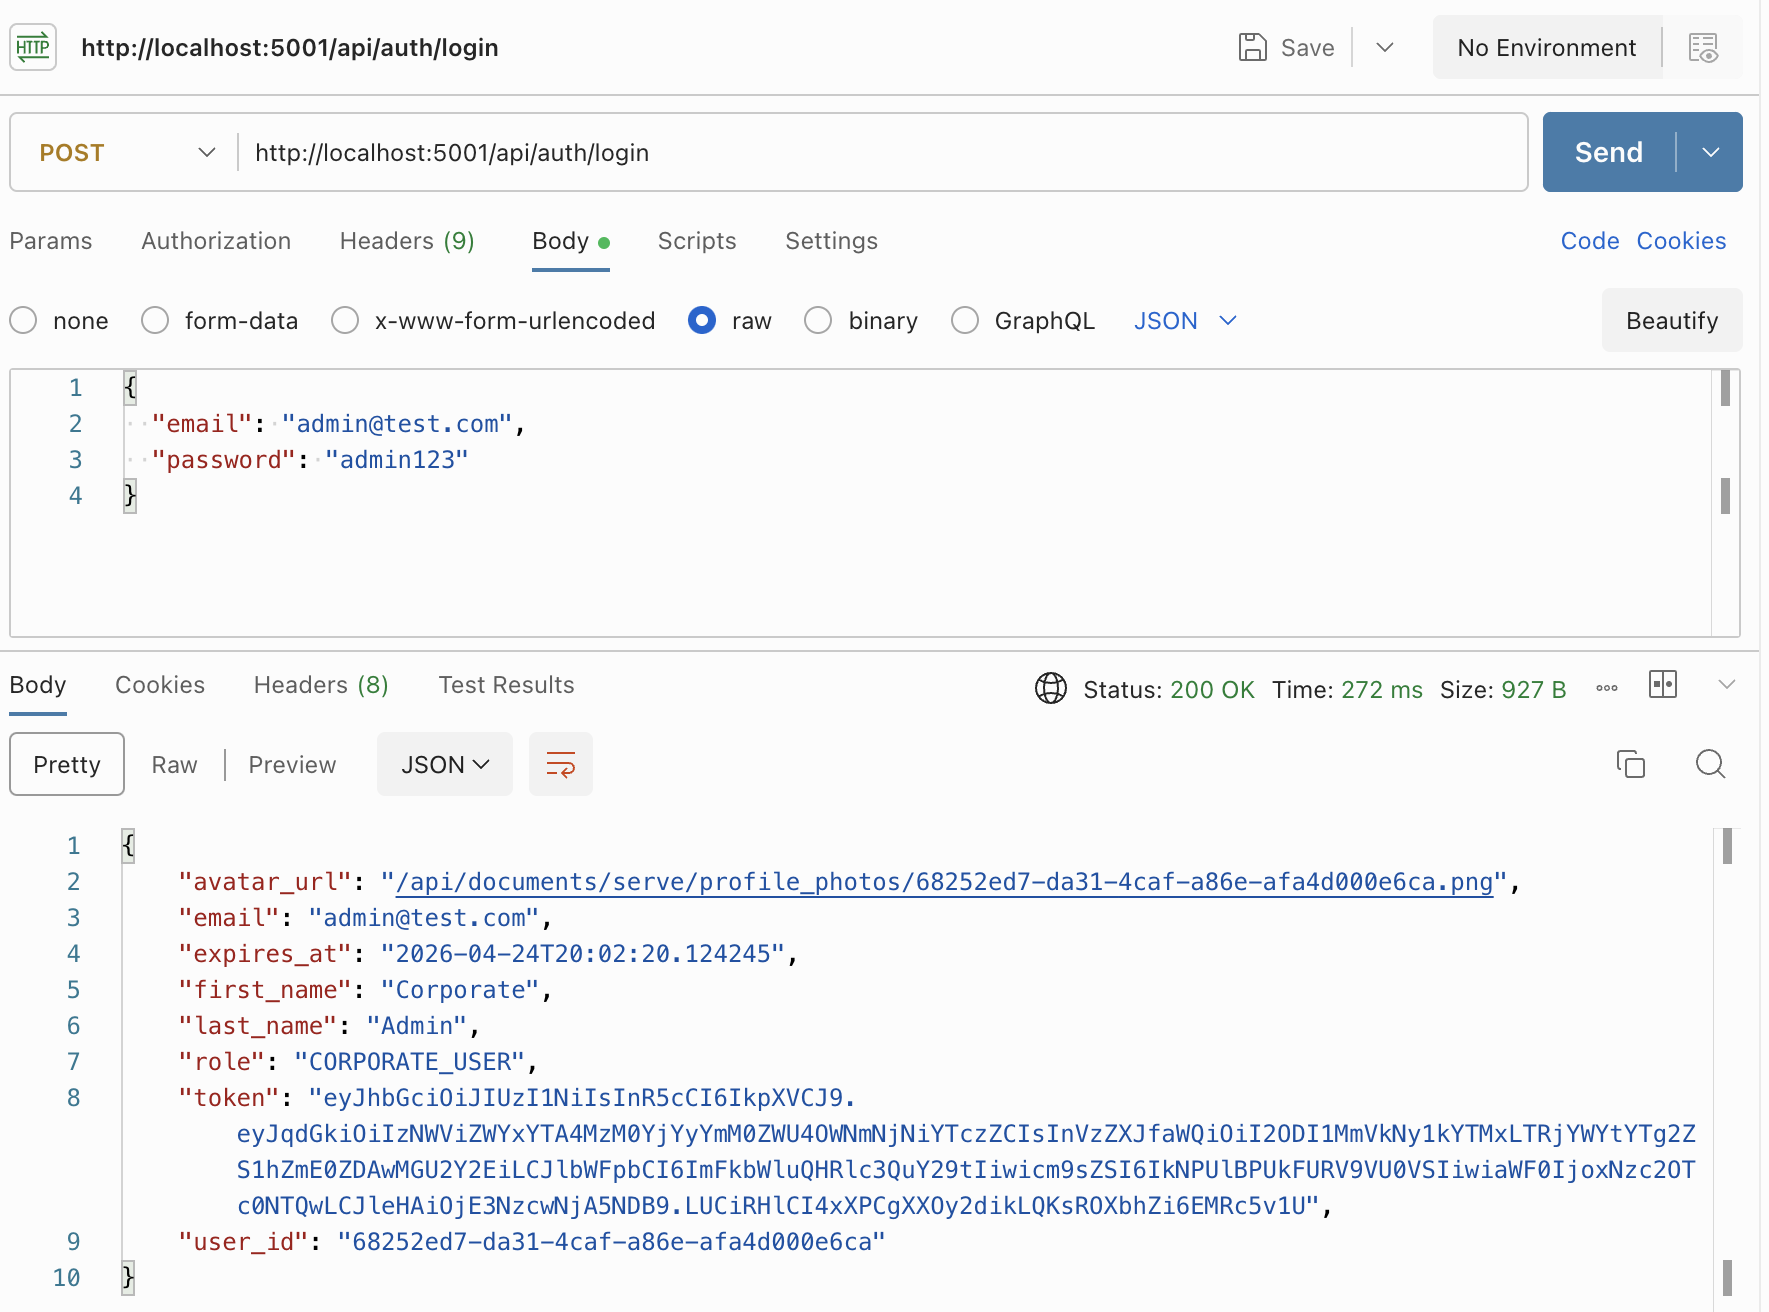
\includegraphics[width=1\linewidth]{figures/chapitre-03/postman-auth-success.png}
  \caption{Tests Postman : authentification réussie.}
  \label{fig:ch3-postman-auth-success}
\end{figure}                 

\begin{figure}[H]
  \centering
  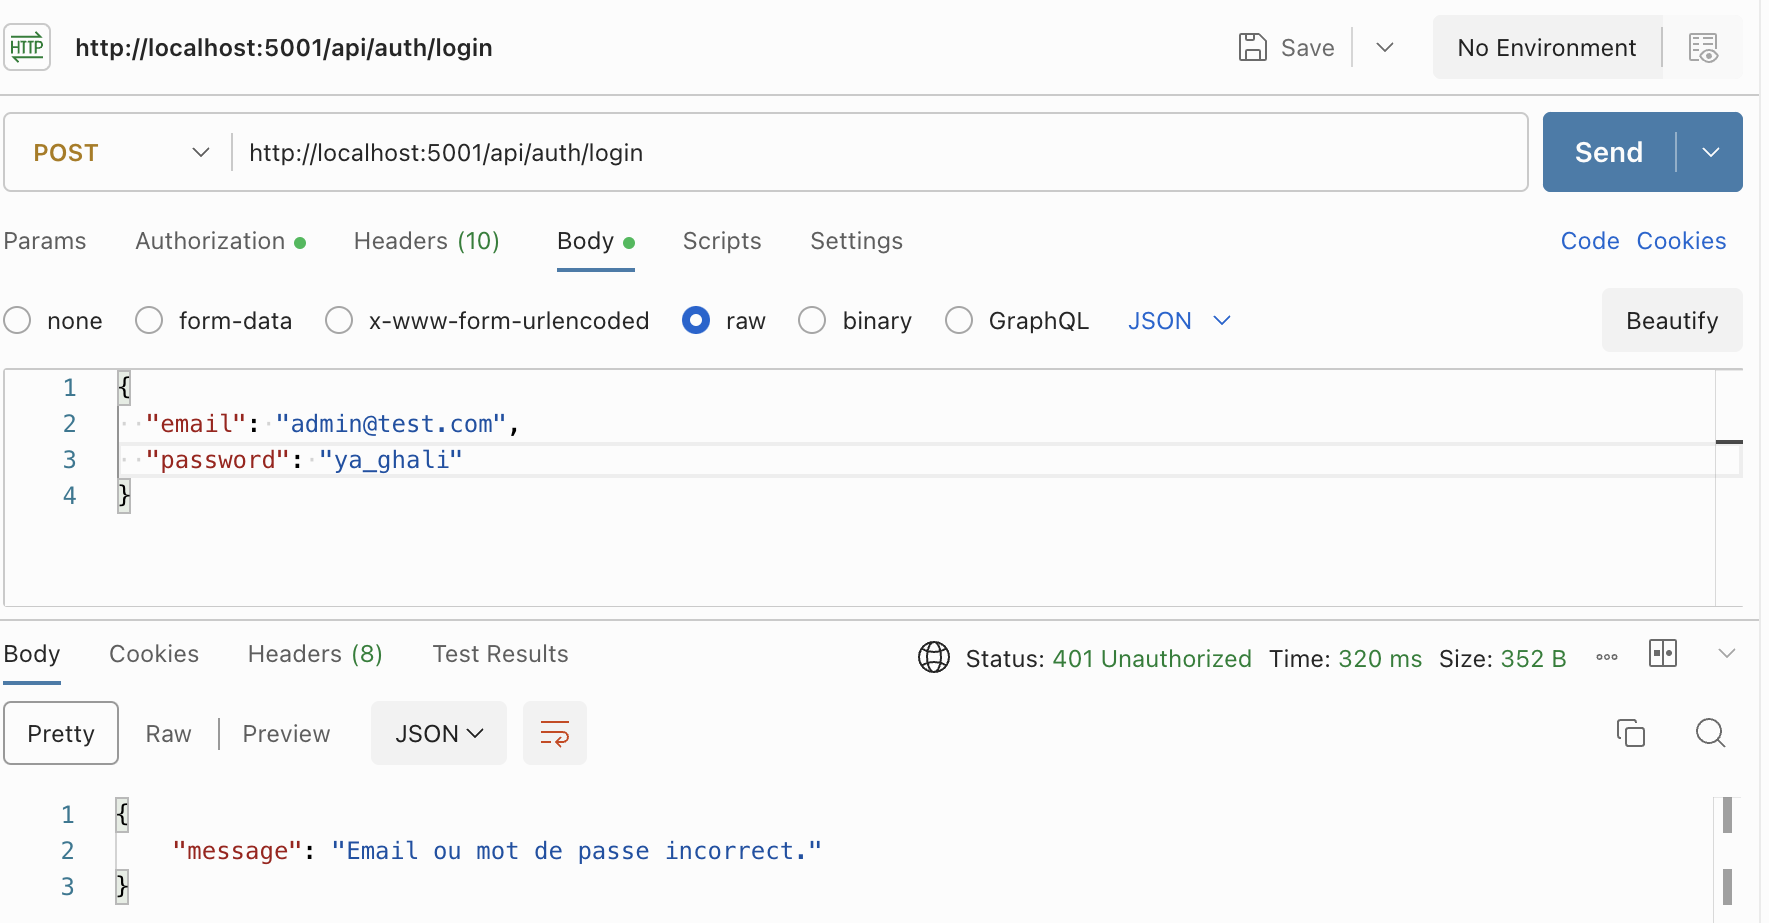
\includegraphics[width=1\linewidth]{figures/chapitre-03/postman-auth-failure.png}
  \caption{Tests Postman : authentification échouée.}
  \label{fig:ch3-postman-auth-failure}
\end{figure}
\subsubsection{Tests création d'un utilisateur}

Les figures~\ref{fig:ch3-postman-user-create-success} et~\ref{fig:ch3-postman-user-create-failure} présentent les cas succès/échec pour la création d'un utilisateur.

Les captures Postman illustrent la vérification du point d’accès \textbf{/api/users} dans deux scénarios complémentaires.
\begin{itemize}
\item Dans le premier cas (succès), l’envoi d’un payload valide pour un nouvel utilisateur retourne le statut \textbf{201 Created} avec les informations du compte créé (identifiant, email, nom, rôle et date de création), ce qui confirme la bonne exécution du processus d’ajout.
\item Dans le second cas (échec), la tentative de création avec un email déjà existant retourne le statut \textbf{409 Conflict} accompagné du message «~Un utilisateur avec cet email existe déjà~», validant le contrôle d’unicité appliqué par l’API.
\end{itemize}

\begin{figure}[H]
  \centering
  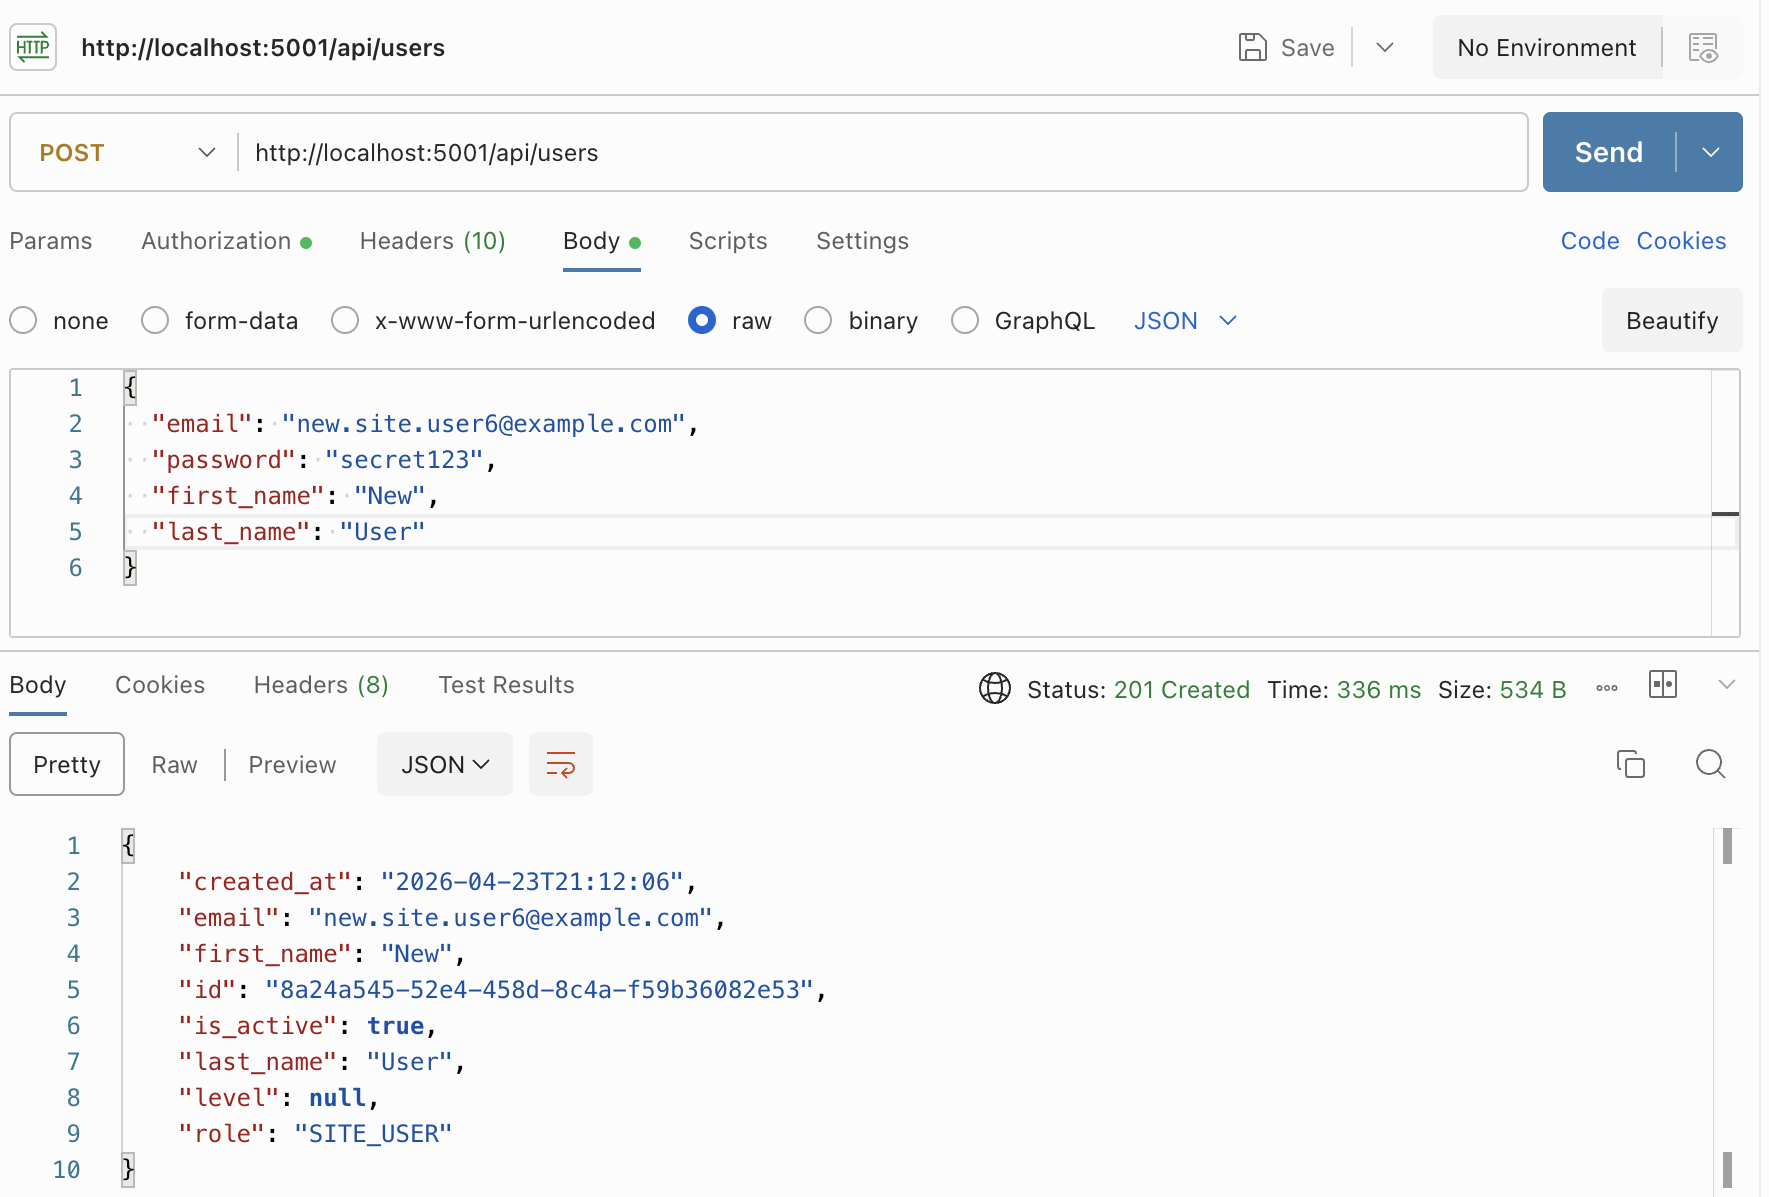
\includegraphics[width=1\linewidth]{figures/chapitre-03/postman-user-create-success.png}
  \caption{Tests Postman : création d'un utilisateur réussie.}
  \label{fig:ch3-postman-user-create-success}
\end{figure}

\begin{figure}[H]
  \centering
  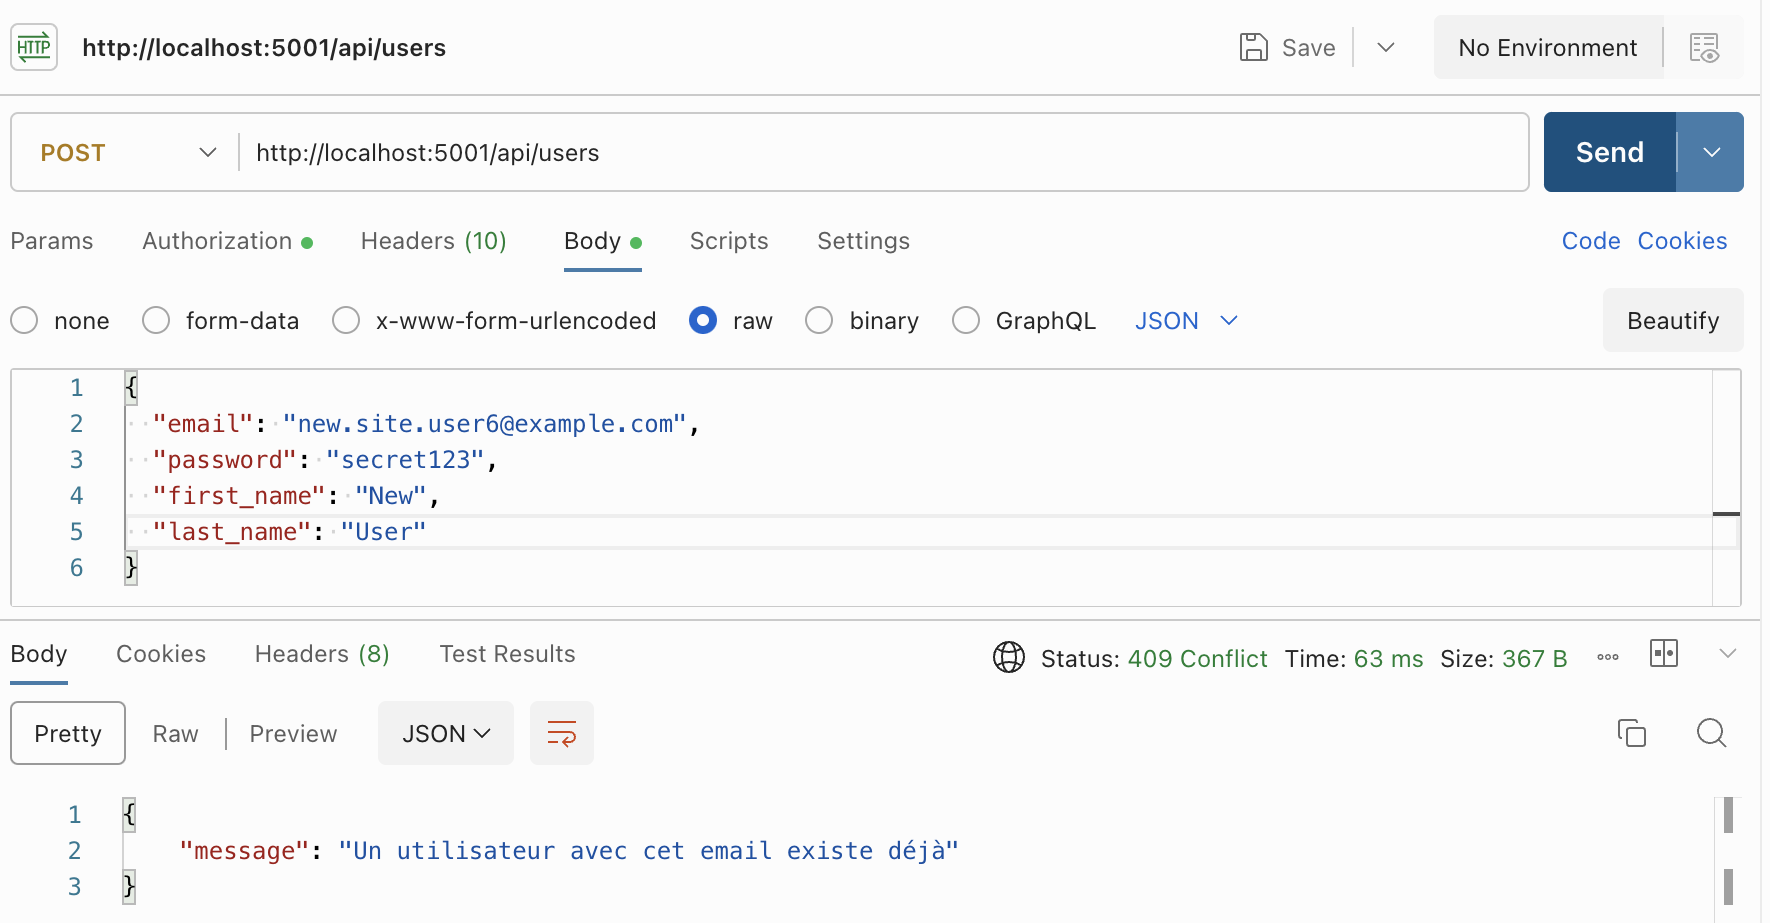
\includegraphics[width=1\linewidth]{figures/chapitre-03/postman-user-create-failure.png}
  \caption{Tests Postman : création d'un utilisateur échouée.}
  \label{fig:ch3-postman-user-create-failure}
\end{figure}


\subsection{Validation}

À la fin du sprint, une réunion de revue a été animée par le \emph{Scrum Master} et le \emph{Product Owner}. Elle a permis de tester les fonctionnalités livrées sur la plateforme CSR (authentification, gestion des utilisateurs, gestion des sites) et de valider leur bon fonctionnement sur les scénarios prioritaires.

Les tests effectués ont confirmé la fiabilité des parcours de gestion des utilisateurs et des sites dans le périmètre de ce sprint. Les éventuels écarts d’affichage ou de formulation signalés lors de la démonstration ont été corrigés afin d’offrir une expérience utilisateur plus claire pour la suite du projet.

\section{Conclusion}

Ce premier sprint a permis de mettre en place les bases essentielles de la plateforme : gestion des utilisateurs, des sites, des accès et des documents. Les fonctionnalités ont été développées et validées, constituant un socle fiable pour la suite du projet.


% Sprint 2 — aligné sur la planification (chapitre 2) et le périmètre « Plans & activités » du product backlog
\PFEChapterOpening{Sprint 2 - Gestion des Plans \& activités}

\section{Introduction}
Ce chapitre présente le deuxième sprint du projet, consacré à la mise en place des fonctionnalités liées aux plans CSR et au suivi des activités. Il marque une étape importante en introduisant le cœur fonctionnel de la plateforme, permettant de structurer les données planifiées et réalisées.
Nous y détaillons les besoins identifiés, les choix de conception adoptés ainsi que les modèles UML utilisés. Des interfaces illustrent également les fonctionnalités développées, accompagnées d’une validation permettant de vérifier leur conformité aux attentes.



\section{Objectif attendu}

Ce deuxième sprint a pour finalité de développer le cœur fonctionnel de la plateforme CSR en mettant en place les modules liés à la planification et au suivi des activités. Il vise à permettre aux utilisateurs de définir les plans annuels CSR par site, de renseigner les activités réalisées tout au long de l’année, et d’assurer un suivi structuré et continu de leur exécution. Ce sprint introduit également des mécanismes de comparaison entre le planifié et le réalisé, afin de mesurer les écarts, d’identifier les dépassements budgétaires et d’évaluer le niveau de réalisation des objectifs fixés. Par ailleurs, il intègre la gestion des activités hors plan, offrant ainsi une meilleure maîtrise opérationnelle. L’ensemble de ces fonctionnalités contribue à renforcer la visibilité sur les performances CSR et constitue une étape clé pour l’exploitation future des données à des fins d’analyse décisionnelle.

\section{Sprint Backlog}

Ce sprint est consacré à la gestion des plans CSR et au suivi des activités, en structurant les informations planifiées et réalisées afin d'assurer un pilotage opérationnel clair au niveau des sites.

Le tableau~\ref{tab:sprint-backlog-2} présente le backlog du deuxième sprint.
% --- Sprint backlog — même style visuel que le product backlog (chapitre 2) ---
% Contenu des user stories / tâches 1.x–6.x issu du tableau Word « Tableau 4.1 » ;
% tâches 1.7–1.10 ajoutées pour refléter le cycle plan côté API (soumission, validation, suppression, bulk).
\small
\PFETableSetup

\setlength{\PFEbacklogTabW}{\dimexpr\textwidth+2.8cm\relax}
\setlength{\LTcapwidth}{\PFEbacklogTabW}
\setlength{\LTleft}{\fill}
\setlength{\LTright}{\fill}

\setlength{\LTpre}{0pt}
\setlength{\LTpost}{0pt}

\PFETableArrayStretch
\setlength{\extrarowheight}{4pt}
\renewcommand{\arraystretch}{1.4}

\arrayrulecolor{black}

\begin{longtable}{|
>{\centering\arraybackslash}m{1.2cm}|
>{\raggedright\arraybackslash}m{5.2cm}|
>{\centering\arraybackslash}m{1.6cm}|
>{\raggedright\arraybackslash}m{5.5cm}|
>{\centering\arraybackslash}m{1.7cm}|}

\caption{Sprint backlog du sprint 2 — Plans \& activités}\label{tab:sprint-backlog-2}\\

\hline
\tableHeaderStyle
\tableHeaderCell{ID} & \tableHeaderCell{User story} & \tableHeaderCell{Tâche ID} & \tableHeaderCell{Tâche} & \tableHeaderCell{Priorité} \\
\hline
\endfirsthead

\hline
\multicolumn{5}{|c|}{\tablename\ \thetable{} — \textit{(suite)}} \\
\hline
\tableHeaderStyle
\tableHeaderCell{ID} & \tableHeaderCell{User story} & \tableHeaderCell{Tâche ID} & \tableHeaderCell{Tâche} & \tableHeaderCell{Priorité} \\
\hline
\endhead

\hline
\multicolumn{5}{|r|}{\textit{Suite page suivante\ldots}} \\
\hline
\endfoot

\hline
\endlastfoot

1 & En tant qu'utilisateur (Site ou Corporate), je veux créer un plan CSR afin de planifier les activités & 1.1 &
Implémenter le module de gestion des plans CSR & +++++ \\
\cline{3-5}
& & 1.2 &
Permettre à l'utilisateur site de créer un plan CSR pour les sites auxquels il est rattaché & +++++ \\
\cline{3-5}
& & 1.3 &
Permettre à l'utilisateur corporate de créer un plan CSR à l'échelle de tous les sites & +++++ \\
\cline{3-5}
& & 1.4 &
Définir les informations du plan (site, année, budget total, \ldots) & +++++ \\
\cline{3-5}
& & 1.5 &
Modifier un plan CSR avant validation & ++++ \\
\cline{3-5}
& & 1.6 &
Consulter les plans CSR par année / statut / site & +++ \\
\cline{3-5}
& & 1.7 &
Soumettre un plan CSR pour validation (passage au statut soumis) & +++++ \\
\cline{3-5}
& & 1.8 &
Permettre à l'utilisateur corporate de valider ou de rejeter un plan soumis avec motif & +++++ \\
\cline{3-5}
& & 1.9 &
Supprimer un plan CSR lorsque les règles métier le permettent & ++++ \\
\cline{3-5}
& & 1.10 &
Soumettre ou supprimer plusieurs plans en une seule opération (actions en masse) & ++++ \\
\cline{3-5}
& & 1.11 &
Rechercher un plan CSR (par mot-clé, site, année) & ++++ \\
\cline{3-5}
& & 1.12 &
Filtrer les plans CSR selon des critères (statut, site, année) & ++++ \\
\cline{3-5}
& & 1.13 &
Soumettre une demande de modification sur un plan verrouillé & ++++ \\
\hline
2 & En tant qu'utilisateur, je veux importer un plan CSR via un fichier Excel afin de gagner du temps & 2.1 &
Implémenter la fonctionnalité d'import Excel & +++++ \\
\cline{3-5}
& & 2.2 &
Lire et parser le fichier Excel avant l'importer & +++++ \\
\cline{3-5}
& & 2.3 &
Valider les données (site, année, mode de validation) pour l'utilisateur site & +++++ \\
\cline{3-5}
& & 2.4 &
Détecter les conflits (doublons, incohérences) & +++++ \\
\cline{3-5}
& & 2.5 &
Afficher un aperçu avant l'importer & ++++ \\
\cline{3-5}
& & 2.6 &
Supprimer les duplicatas avant la validation & ++++ \\
\cline{3-5}
& & 2.7 &
Ignorer les duplicatas et continuer avant la validation & ++++ \\
\hline
3 & En tant qu'utilisateur Site, je veux gérer les activités planifiées afin d'organiser les actions CSR & 3.1 &
Ajouter une méthode pour ajouter activité planifiée & +++++ \\
\cline{3-5}
& & 3.2 &
Ajouter les informations nécessaires de chaque activité planifiée(titre,numéro, catégorie, budget prévu, Impact de l'action prévue \ldots) & +++++ \\
\cline{3-5}
& & 3.3 &
Ajouter une méthode de  modification de l'activité planifiée avant validation & ++++ \\
\cline{3-5}
& & 3.4 &
Ajouter une méthode de suppression de l'activité planifiée avant validation & ++++ \\
\cline{3-5}
& & 3.5 &
Ajouter une méthode de consultation du détail d'une activité planifiée & ++++ \\
\cline{3-5}
& & 3.6 &
Ajouter une fonctionnalité de recherche des activités planifiées & ++++ \\
\cline{3-5}
& & 3.7 &
Ajouter une fonctionnalité de filtrage des activités planifiées & ++++ \\
\hline
4 & En tant qu'utilisateur Site, je veux saisir les activités réalisées afin de suivre l'exécution & 4.1 &
Implémenter le module des activités réalisées & +++++ \\
\cline{3-5}
& & 4.2 &
Ajouter une méthode pour saisir  les données de l'activité réalisée( Budget réalisé, participants, Date de réalisation, \ldots) & +++++ \\
\cline{3-5}
& & 4.3 &
Ajouter une méthode de  modification de l'activité réalisée & ++++ \\
\cline{3-5}
& & 4.4 &
Ajouter une méthode de suppression de l'activité réalisée & ++++ \\
\cline{3-5}
& & 4.5 &
Ajouter une méthode de consultation du détail d'une activité réalisée & ++++ \\
\cline{3-5}
& & 4.6 &
Ajouter une fonctionnalité de recherche des activités réalisées & ++++ \\
\cline{3-5}
& & 4.7 &
Ajouter une fonctionnalité de filtrage des activités réalisées & ++++ \\
\hline
5 & En tant qu'utilisateur Site, je veux ajouter des activités hors plan afin de tracer les actions imprévues & 5.1 &
Ajouter une méthode de création d'une activité hors plan & +++++ \\
\cline{3-5}
& & 5.2 &
Saisir toutes les informations de l'activité hors plan (titre, catégorie, date de réalisation, \ldots) & +++++ \\
\cline{3-5}
& & 5.3 &
Ajouter une méthode de  modification de l'activité hors plan & ++++ \\
\cline{3-5}
& & 5.4 &
Ajouter une méthode de suppression de l'activité hors plan & ++++ \\
\cline{3-5}
& & 5.5 &
Soumettre une activité hors plan pour validation & ++++ \\
\hline
6 & En tant qu'utilisateur, je veux visualiser les informations planifiées et réalisées afin d'avoir une vue complète & 6.1 &
Afficher les données planifiées( Budget prévu, impact prévu de l'action, nombre de participants prévus, \ldots) & +++++ \\
\cline{3-5}
& & 6.2 &
Afficher les données réalisées( Budget réalisé, impact de l'action , nombre réel de participants, \ldots) & +++++ \\
\hline

\end{longtable}

\normalsize

\newpage
\section{Analyse détaillée des besoins}

\subsection{Diagramme de cas d'utilisation}

La figure~\ref{fig:doc-ch4-1} illustre le diagramme de cas d'utilisation du deuxième sprint.

\IfFileExists{figures/chapitre-04/diagramme-cas-utilisation-plans-activites.png}{%
\begin{figure}[H]
  \centering
  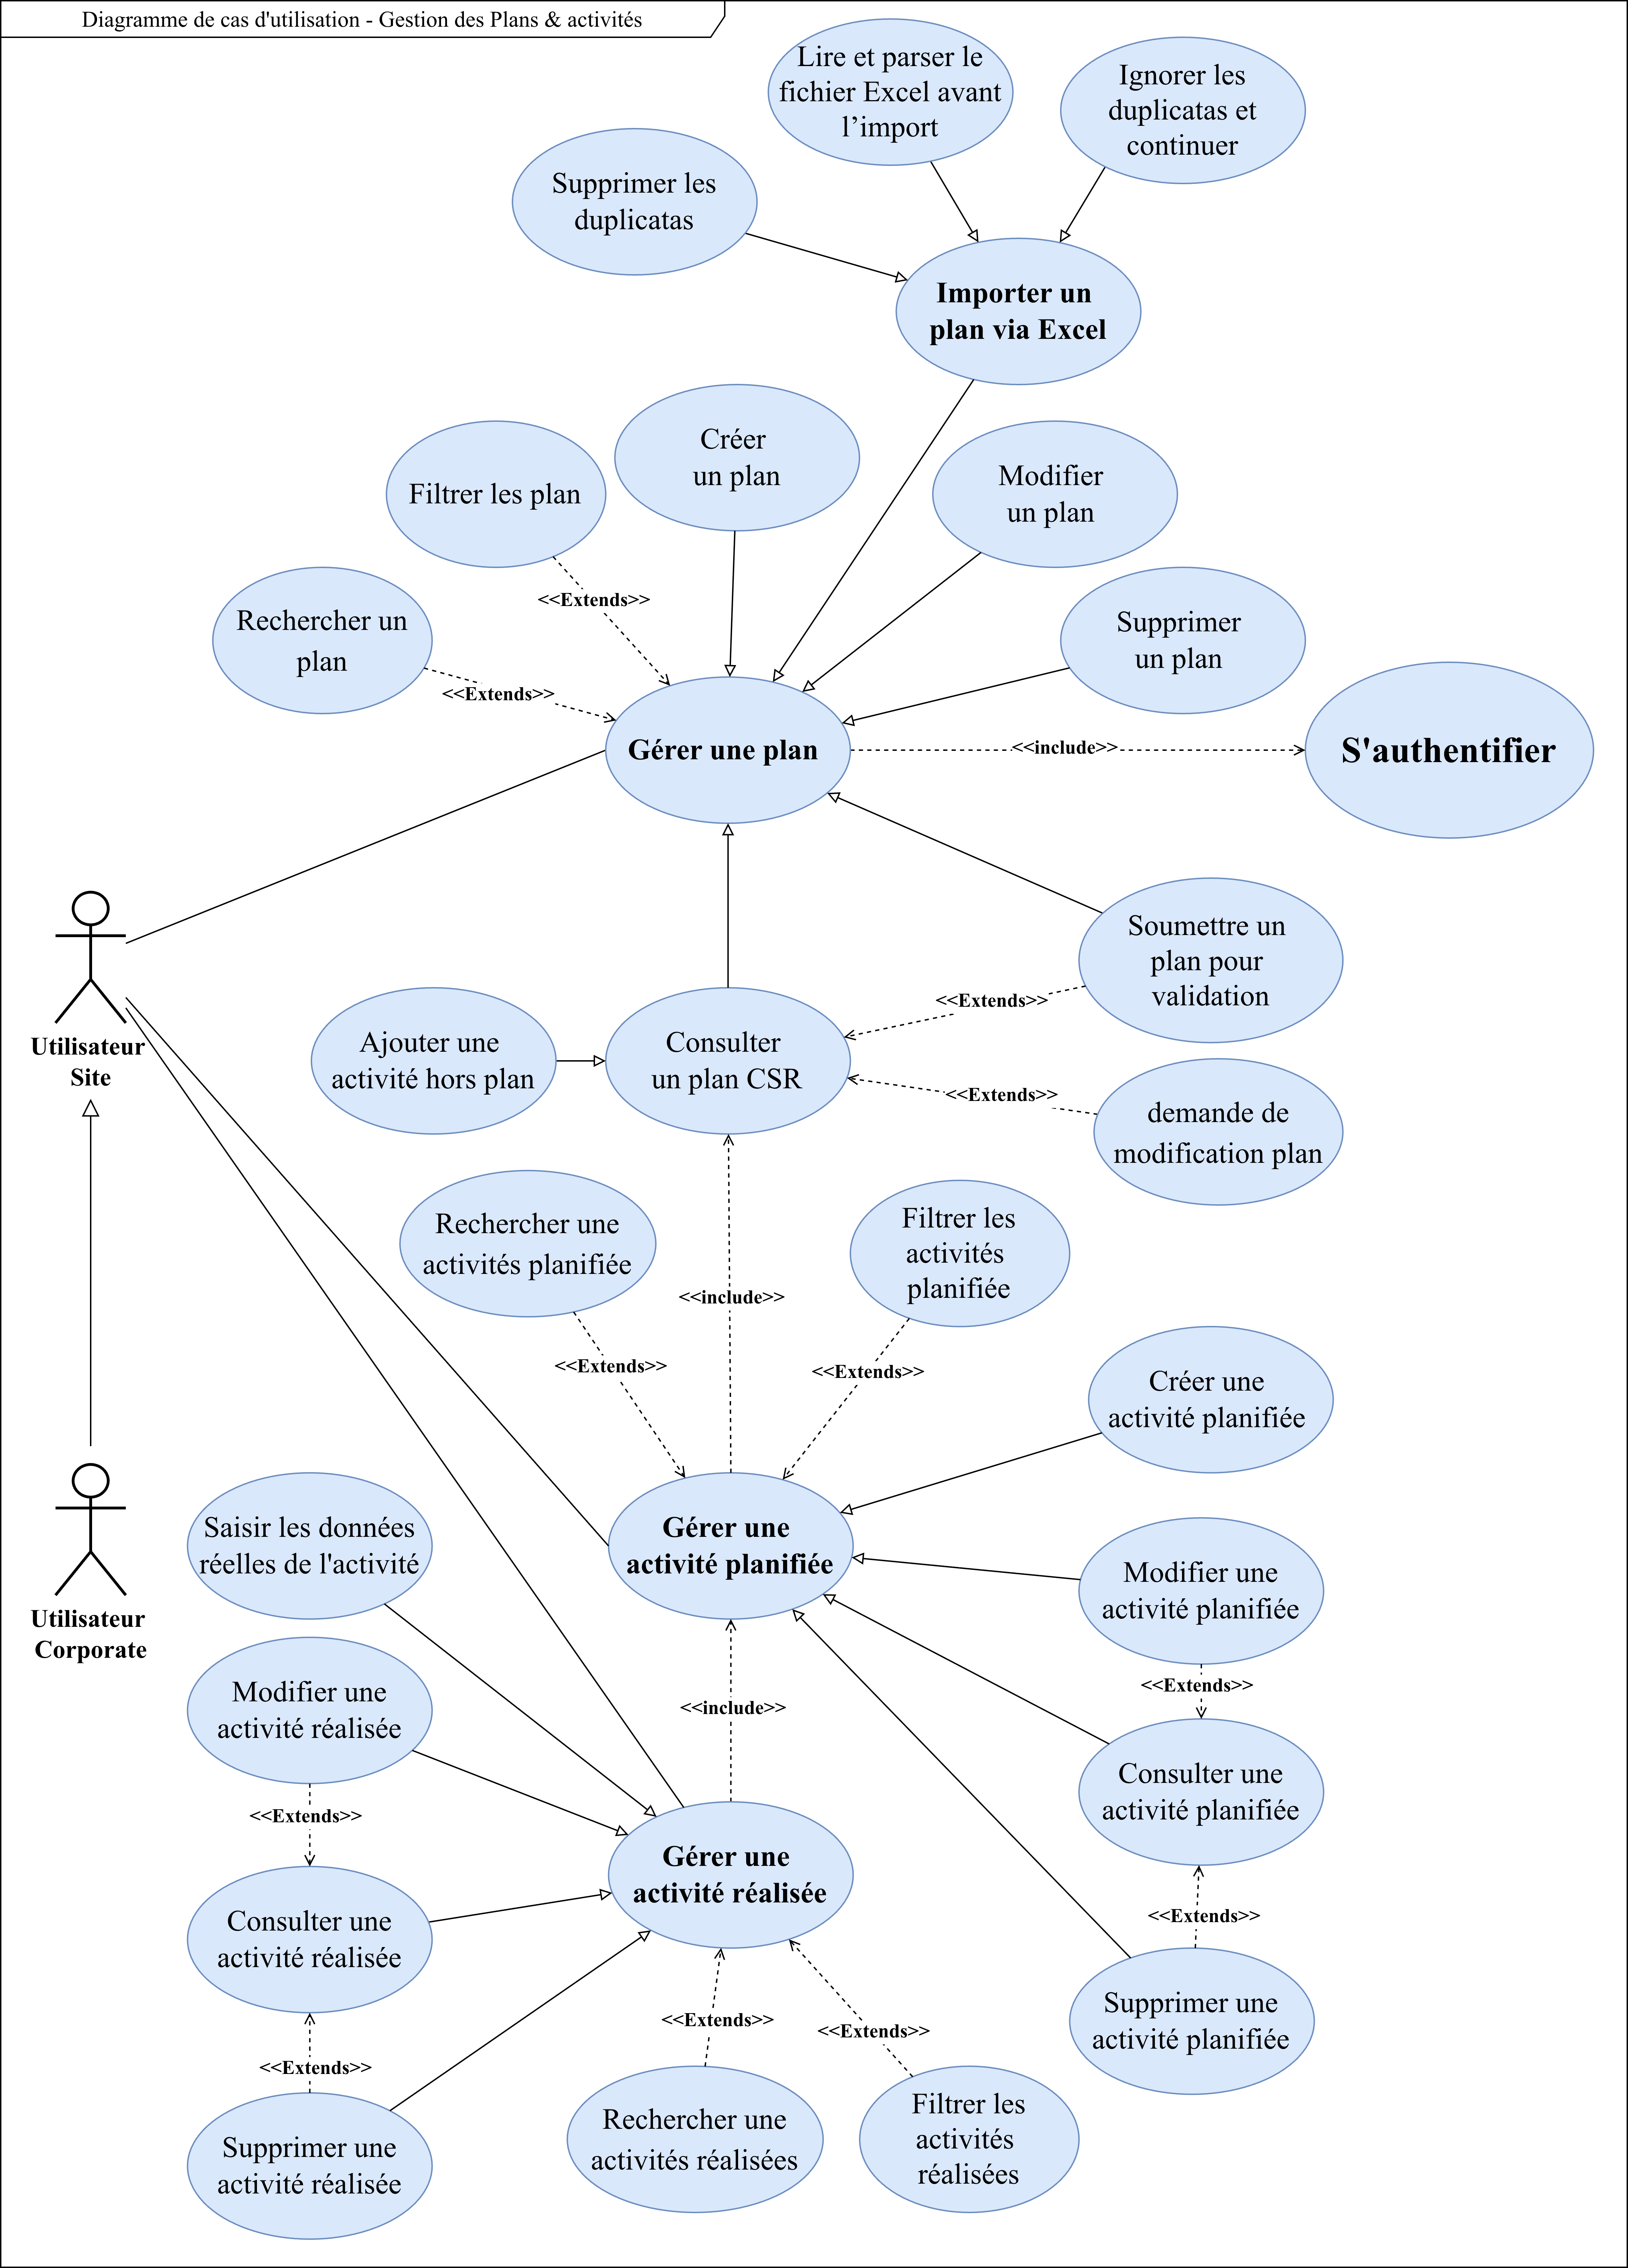
\includegraphics[width=0.92\linewidth]{figures/chapitre-04/diagramme-cas-utilisation-plans-activites.png}
  \caption{Diagramme de cas d'utilisation du deuxième sprint.}
  \label{fig:doc-ch4-1}
\end{figure}%
}{%
\begin{figure}[H]
  \centering
  \fbox{\parbox{0.92\linewidth}{\centering\vspace{3.2cm}\textit{(Figure à insérer : \texttt{figures/chapitre-04/diagramme-cas-utilisation-plans-activites.png})}\vspace{3.2cm}}}
  \caption{Diagramme de cas d'utilisation du deuxième sprint.}
  \label{fig:doc-ch4-1}
\end{figure}%
}
\newpage

\subsection{Description textuelle du cas d'utilisation : «~Créer un plan CSR~»}

Le tableau~\ref{tab:cu-creer-plan-csr} expose la description textuelle du cas d'utilisation «~Créer un plan CSR~».

% Cas d'utilisation « Créer un plan CSR » — inclus sous la sous-section 4.4.2
\begin{table}[H]
  \centering
  \small
  \caption{Description textuelle du cas d'utilisation : «~Créer un plan CSR~»}
  \label{tab:cu-creer-plan-csr}
  \PFETableSetup
  \PFETableRowColors
  \PFETableArrayStretch
  \PFETableTabularXBegin
  \begin{tabularx}{\PFETableBlockWidth}{@{}>{\raggedright\arraybackslash}p{3.2cm} >{\raggedright\arraybackslash}X@{}}
    \tableHeaderStyle \tableHeaderCell{Champ} & \tableHeaderCell{Contenu} \\
    \textbf{Titre} & Créer un plan CSR \\
    \textbf{Acteurs} & Utilisateur Corporate ; utilisateur Site. \\
    \textbf{Objectif} &
      Permettre aux utilisateurs de définir un plan CSR annuel afin de structurer la planification des activités et organiser les initiatives au niveau des sites. \\
    \textbf{Préconditions} &
      1. L'utilisateur est authentifié.\par
      2. Un token est obtenu pour accéder aux ressources protégées. \\
    \textbf{Postconditions} &
      1. Les informations du plan (site, année, budget, etc.) sont sauvegardées.\par
      2. Le plan devient disponible pour l'ajout des activités. \\
    \textbf{Scénario nominal} &
      1. L'utilisateur accède au module des plans CSR.\par
      2. Le système affiche les plans existants.\par
      3. L'utilisateur sélectionne l'option de création d'un plan.\par
      4. Il saisit les informations du plan (site(s), année, budget total, etc.).\par
      5. Le système vérifie la validité des données.\par
      6. Le système enregistre le plan CSR.\par
      7. Le plan apparaît dans la liste des plans disponibles. \\
    \textbf{Scénario alternatif} &
      \textbf{A. Plan déjà existant :} \par
      A.1 L'utilisateur tente de créer un plan pour un site et une année déjà existants. \par
      A.2 Le système rejette l'opération. \par
      A.3 Un message est affiché : «~Un plan existe déjà pour ce site et cette année~». \par\medskip
      \textbf{B. Données invalides :} \par
      B.1 L'utilisateur saisit des informations incomplètes. \par
      B.2 Le système bloque la création du plan. \par
      B.3 Un message d'erreur s'affiche en fonction des informations manquantes. \\
  \end{tabularx}%
  \PFETableTabularXEnd
\end{table}

\newpage

\subsection{Description textuelle du cas d'utilisation : «~Soumettre un plan CSR pour validation~»}

Le tableau~\ref{tab:cu-soumettre-plan-csr} expose la description textuelle du cas d'utilisation «~Soumettre un plan CSR pour validation~».

% Cas d'utilisation « Soumettre un plan CSR pour validation » — inclus sous la sous-section 4.4.3
\begin{table}[H]
  \centering
  \small
  \caption{Description textuelle du cas d'utilisation : «~Soumettre un plan CSR pour validation~»}
  \label{tab:cu-soumettre-plan-csr}
  \PFETableSetup
  \PFETableRowColors
  \PFETableArrayStretch
  \PFETableTabularXBegin
  \begin{tabularx}{\PFETableBlockWidth}{@{}>{\raggedright\arraybackslash}p{3.2cm} >{\raggedright\arraybackslash}X@{}}
    \tableHeaderStyle \tableHeaderCell{Champ} & \tableHeaderCell{Contenu} \\
    \textbf{Titre} & Soumettre un plan CSR pour validation \\
    \textbf{Acteurs} & Utilisateur Corporate ; utilisateur Site. \\
    \textbf{Objectif} &
      Permettre à l'utilisateur de soumettre un plan CSR afin de lancer le processus de validation et de figer les informations avant son exécution. \\
    \textbf{Préconditions} &
      1. L'utilisateur est authentifié.\par
      2. Un token est obtenu pour accéder aux ressources protégées.\par
      3. Un plan CSR existe.\par
      4. Le plan est complet et en état modifiable. \\
    \textbf{Postconditions} &
      1. Le plan CSR passe à l'état «~soumis~».\par
      2. Il devient non modifiable selon les règles métier.\par
      3. Il est prêt pour le processus de validation.\par
      4. Une notification est envoyée à l'utilisateur corporate. \\
    \textbf{Scénario nominal} &
      1. L'utilisateur accède au module des plans CSR.\par
      2. Le système affiche la liste des plans existants.\par
      3. L'utilisateur sélectionne un plan.\par
      4. Le système affiche les détails du plan.\par
      5. L'utilisateur déclenche l'action de soumission.\par
      6. Le système vérifie que les informations requises sont complètes.\par
      7. Le système change le statut du plan en «~soumis~».\par
      8. Le système enregistre la modification. \\
    \textbf{Scénario alternatif} &
      \textbf{A. Données incomplètes :} \par
      A.1 Le système refuse la soumission. \par
      A.2 Il signale les champs ou règles non satisfaits. \par\medskip
      \textbf{B. Plan non modifiable :} \par
      B.1 Le système informe l'utilisateur que la soumission n'est pas possible. \par
      B.2 Le message indique la cause (statut, droits ou fenêtre de modification). \\
  \end{tabularx}%
  \PFETableTabularXEnd
\end{table}


\section{Modélisation conceptuelle}

Dans cette section, nous détaillons les choix de conception adoptés pour le \textbf{deuxième sprint}. Nous y présentons d'abord le diagramme de classes, puis nous illustrons les principaux cas d'utilisation à travers des diagrammes de séquence, afin d'expliciter les interactions entre les composants du système.

\subsection{Diagramme de classe}


La figure~\ref{fig:doc-ch4-2} représente le diagramme de classe du deuxième sprint.

\begin{figure}[H]
  \centering
  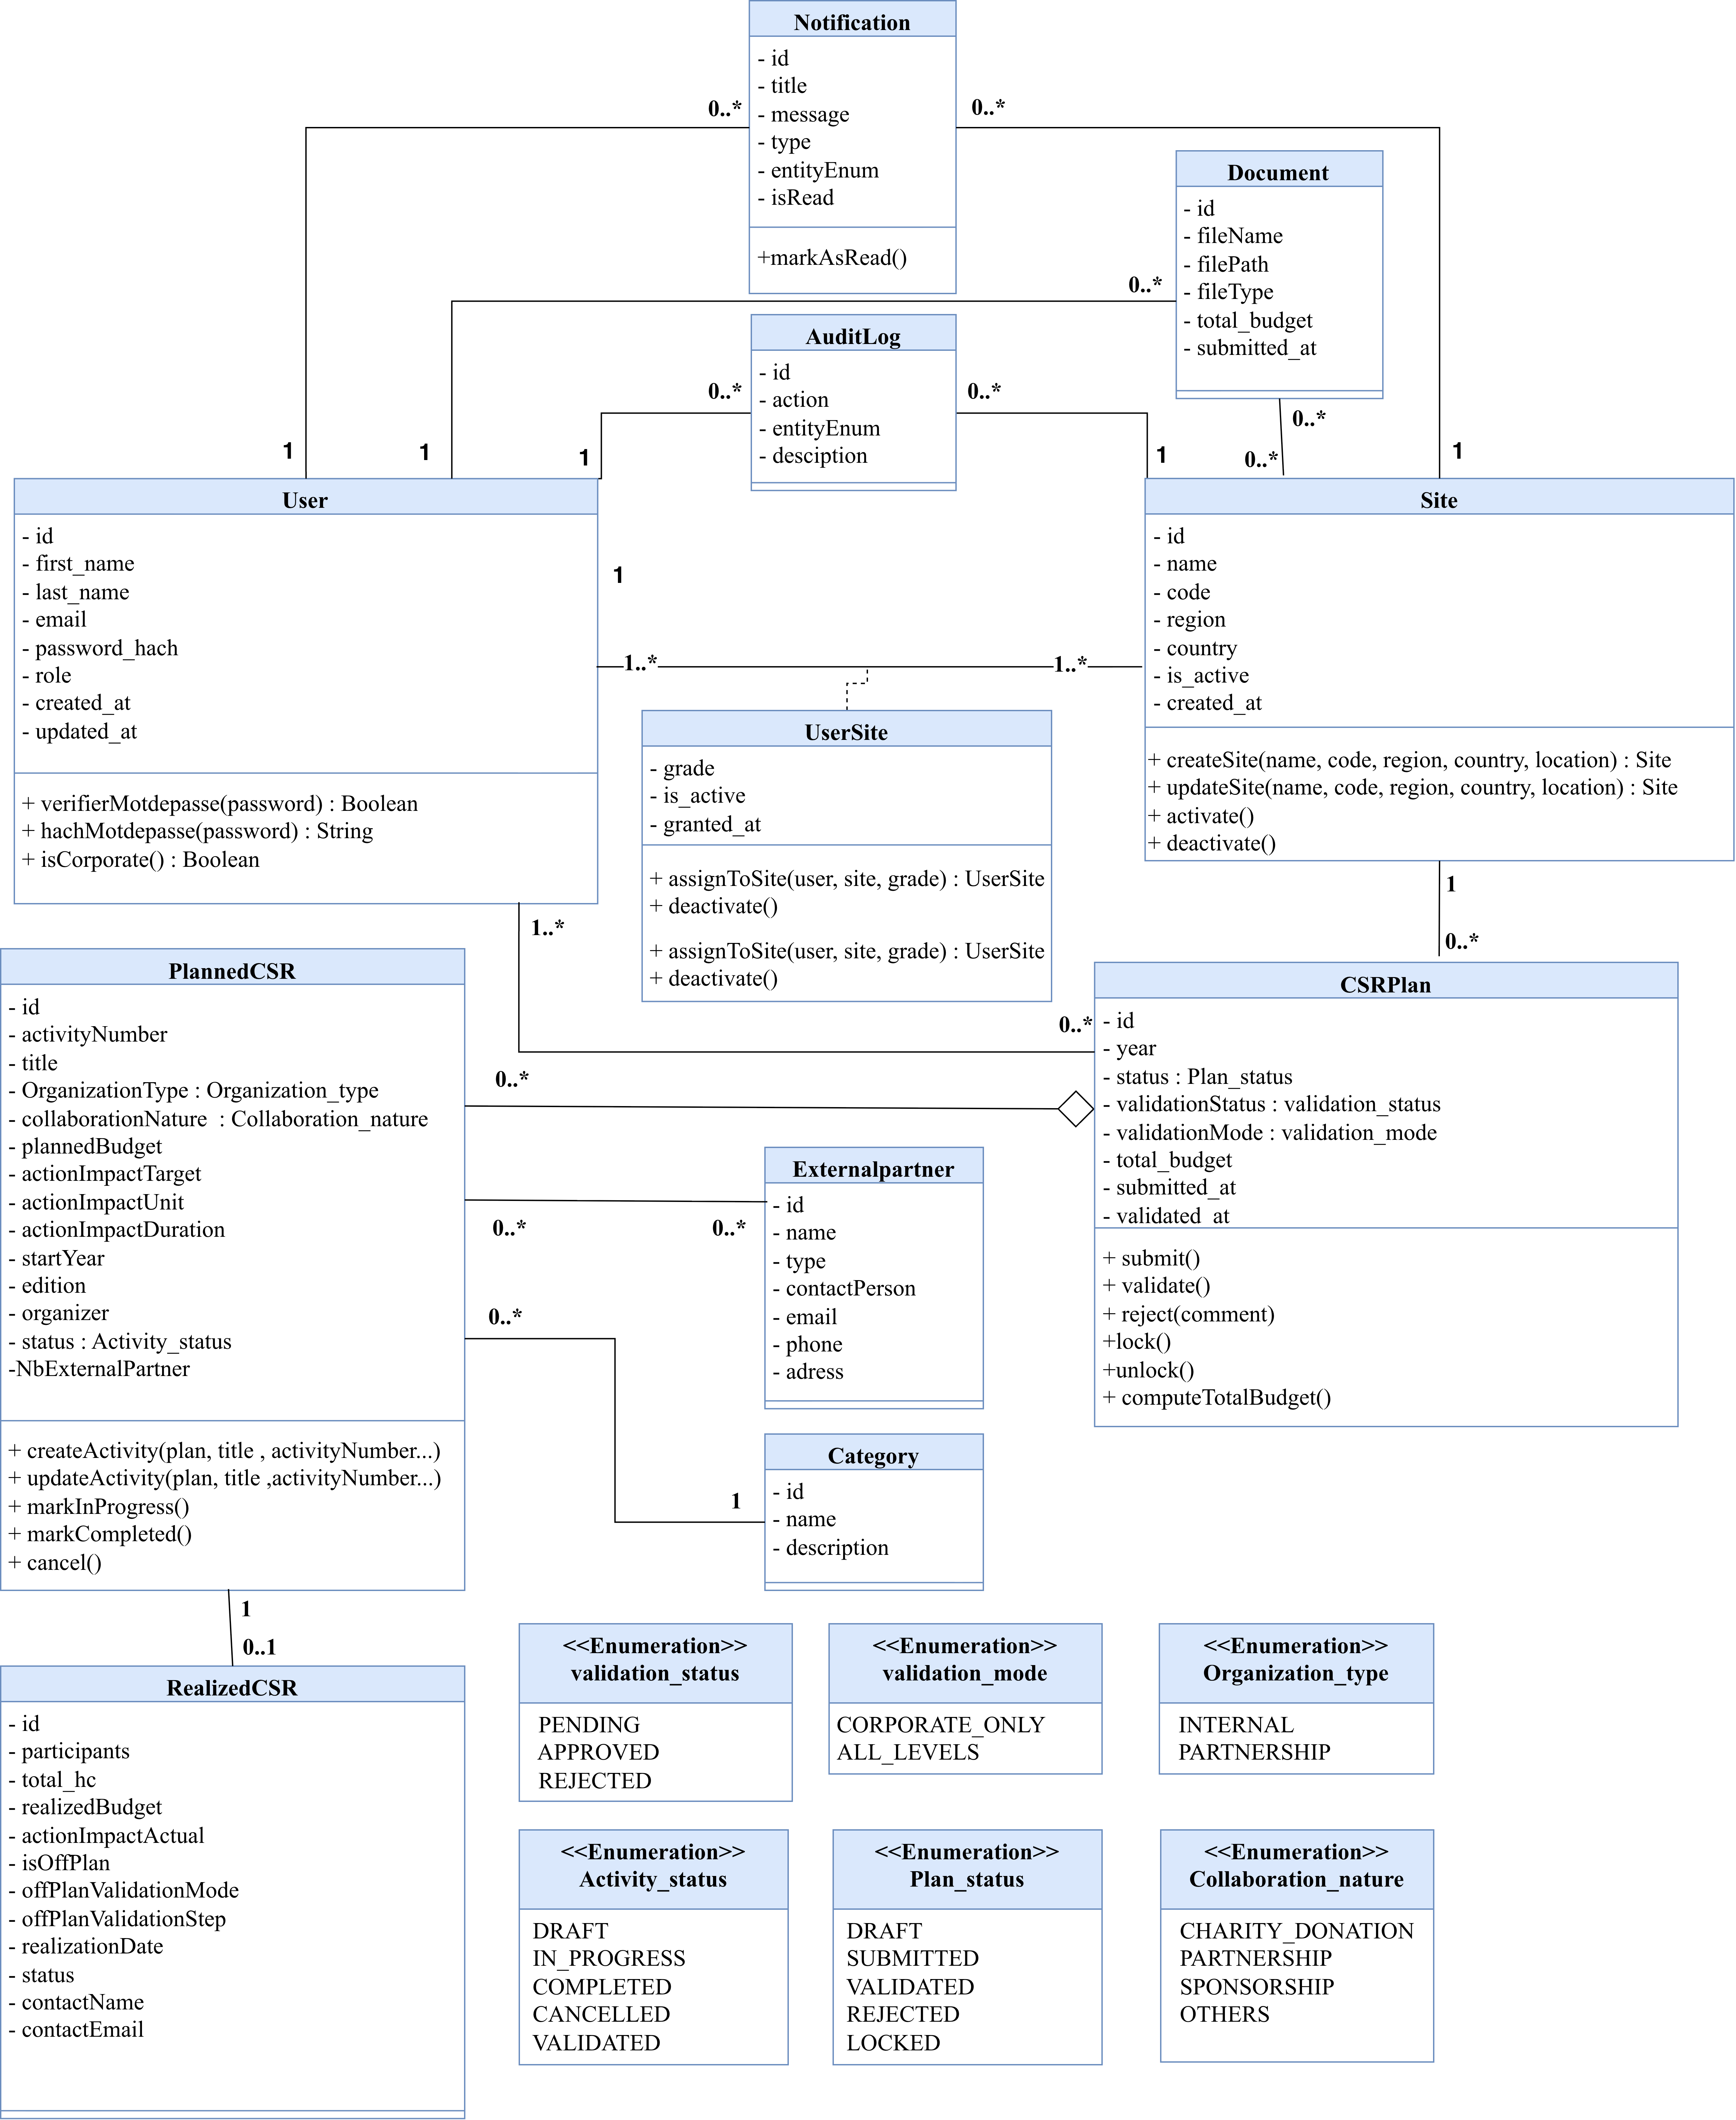
\includegraphics[width=0.82\linewidth]{figures/chapitre-04/diagramme-classe-plans-activites.png}
  \caption{Diagramme de classe -- Gestion des plans \& activités.}
  \label{fig:doc-ch4-2}
\end{figure}%


\subsection{Diagramme de séquence}

Les diagrammes de séquence décrivent les interactions dynamiques entre les composants du système. Nous détaillons ici deux scénarios essentiels du sprint~: la \textbf{création d'un plan CSR} et la \textbf{modification d'une activité planifiée}.        

\subsubsection{Diagramme de séquence : «~Créer un plan CSR~»}

La figure~\ref{fig:doc-ch4-seq-creer-plan} présente le scénario «~Créer un plan CSR~».

\begin{figure}[H]
  \centering
  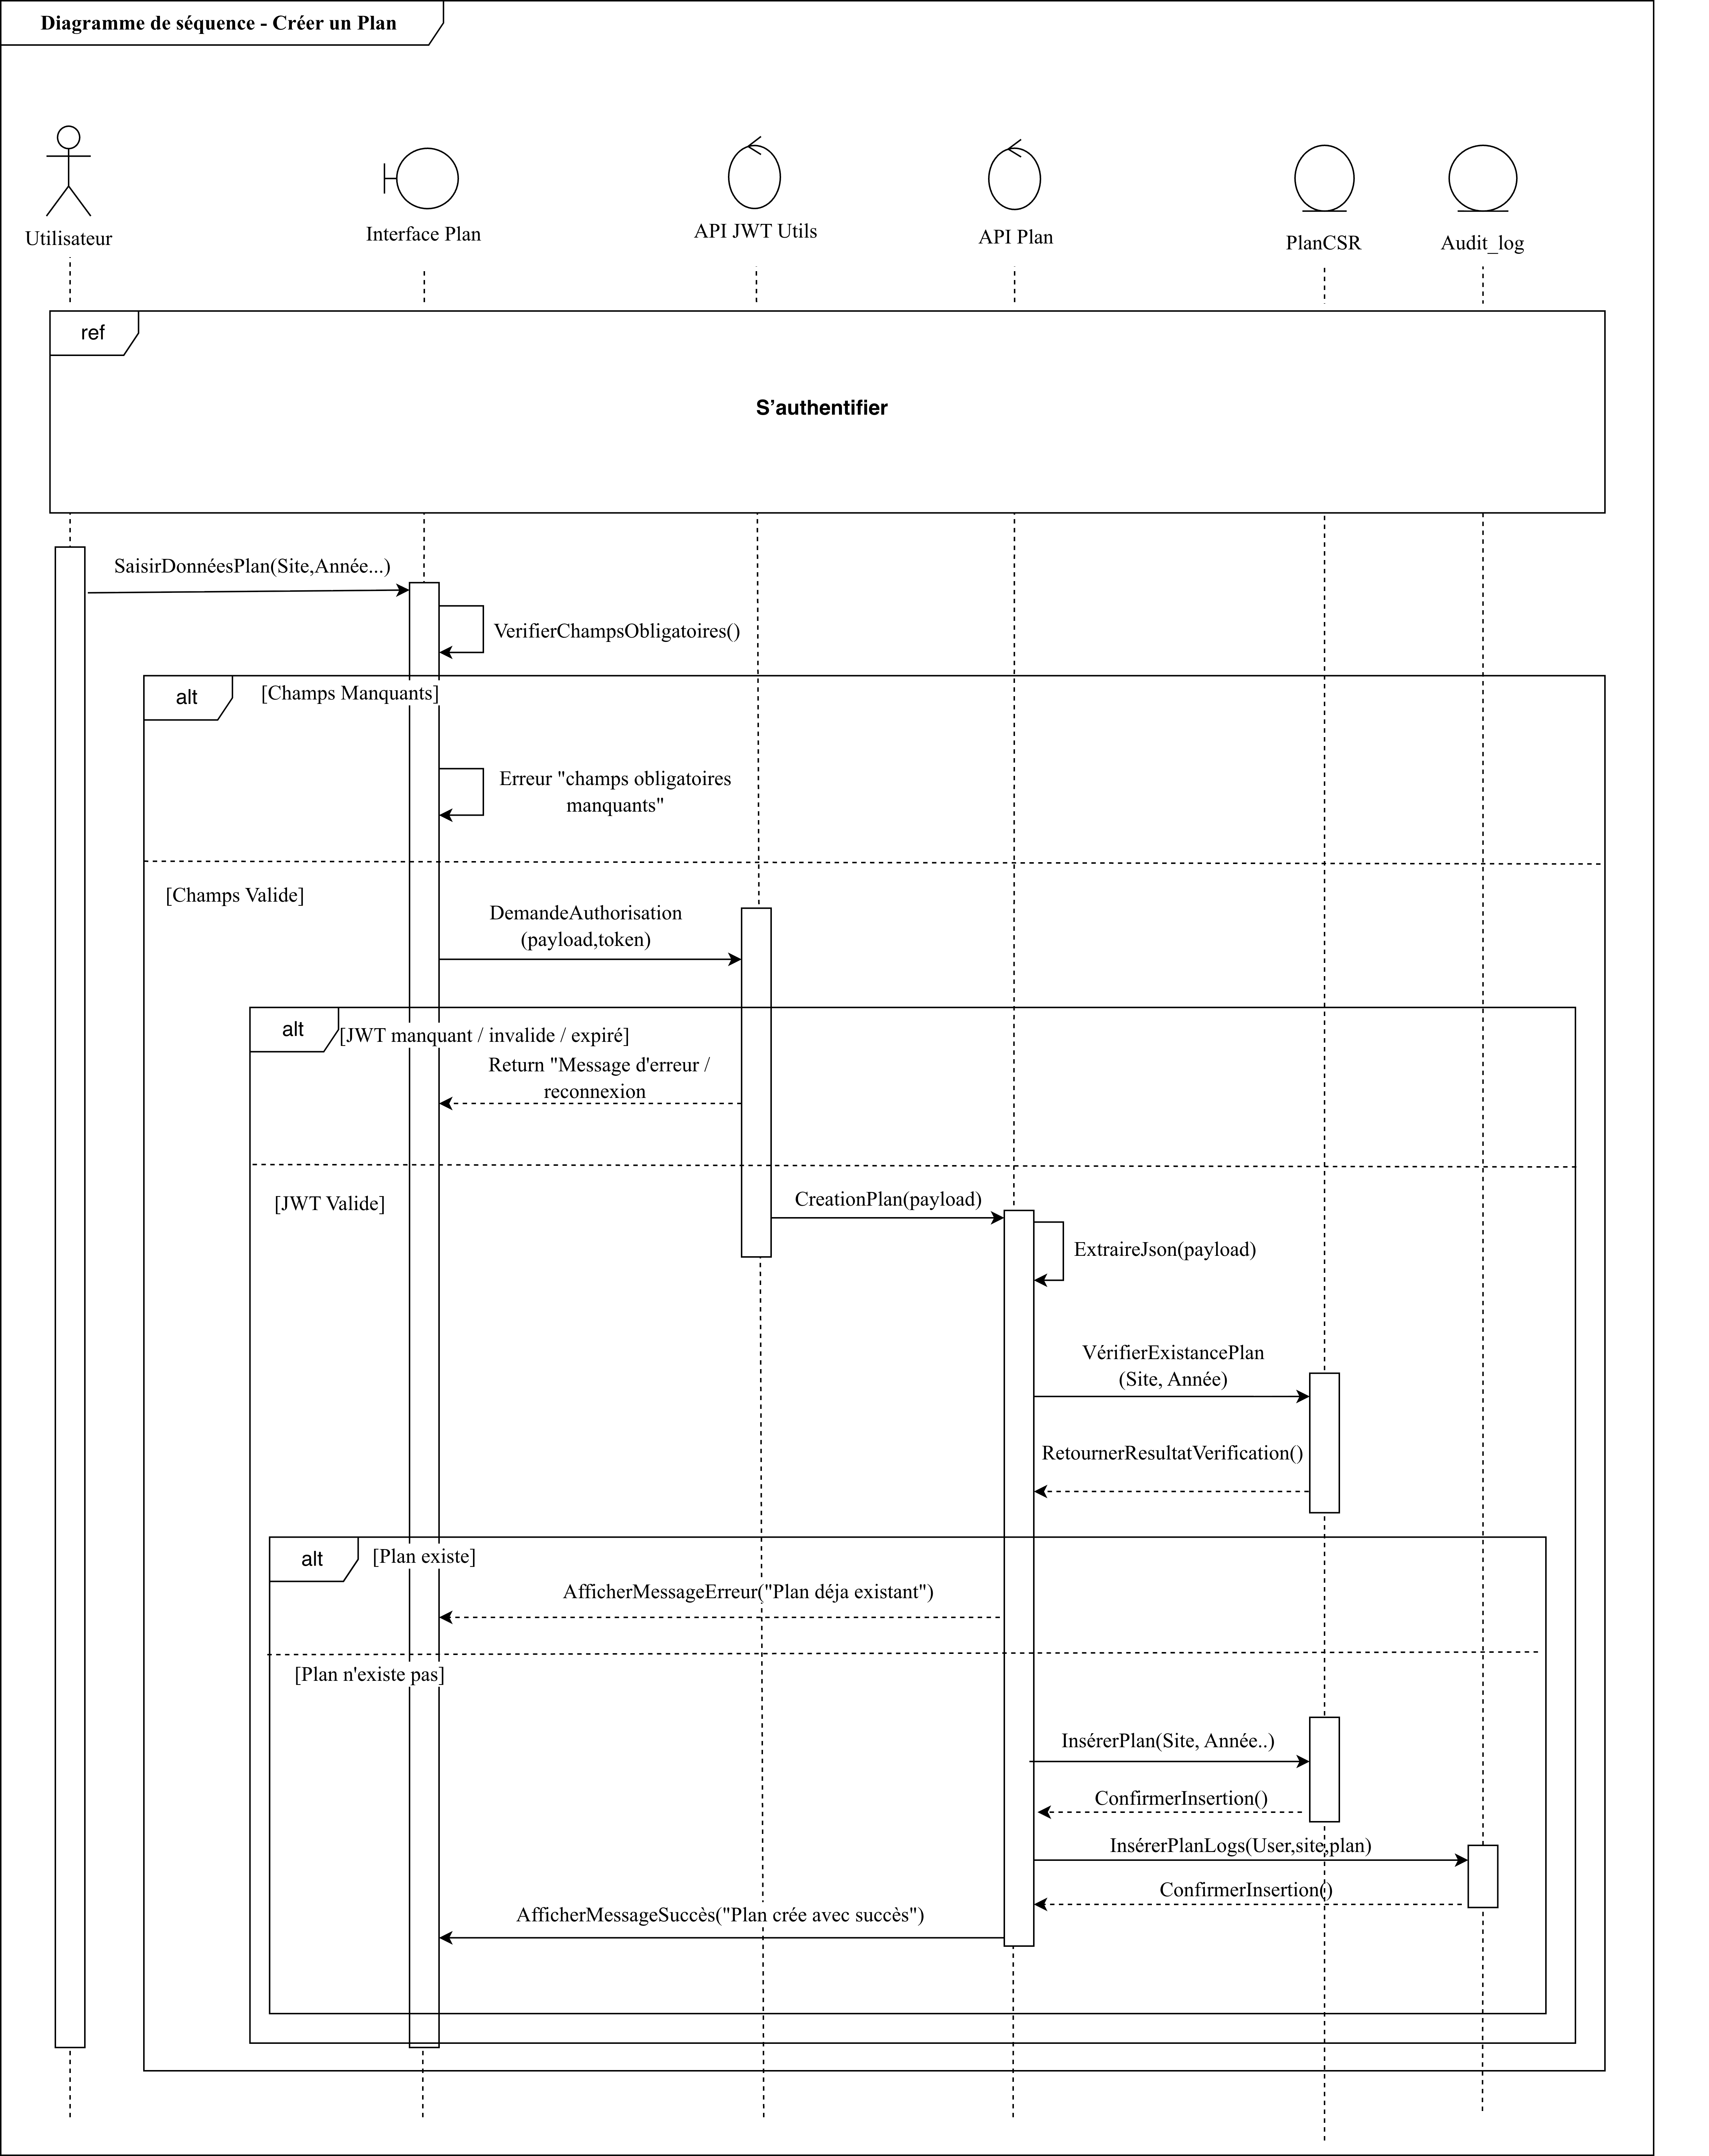
\includegraphics[width=0.92\linewidth]{figures/chapitre-04/diagramme-sequence-creer-plan-csr.png}
  \caption{Diagramme de séquence — «~Créer un plan CSR~».}
  \label{fig:doc-ch4-seq-creer-plan}
\end{figure}

\subsubsection{Diagramme de séquence : «~Modifier une activité planifiée~»}

La figure~\ref{fig:doc-ch4-seq-modif-activite} présente le scénario «~Modifier une activité planifiée~».

\begin{figure}[H]
  \centering
  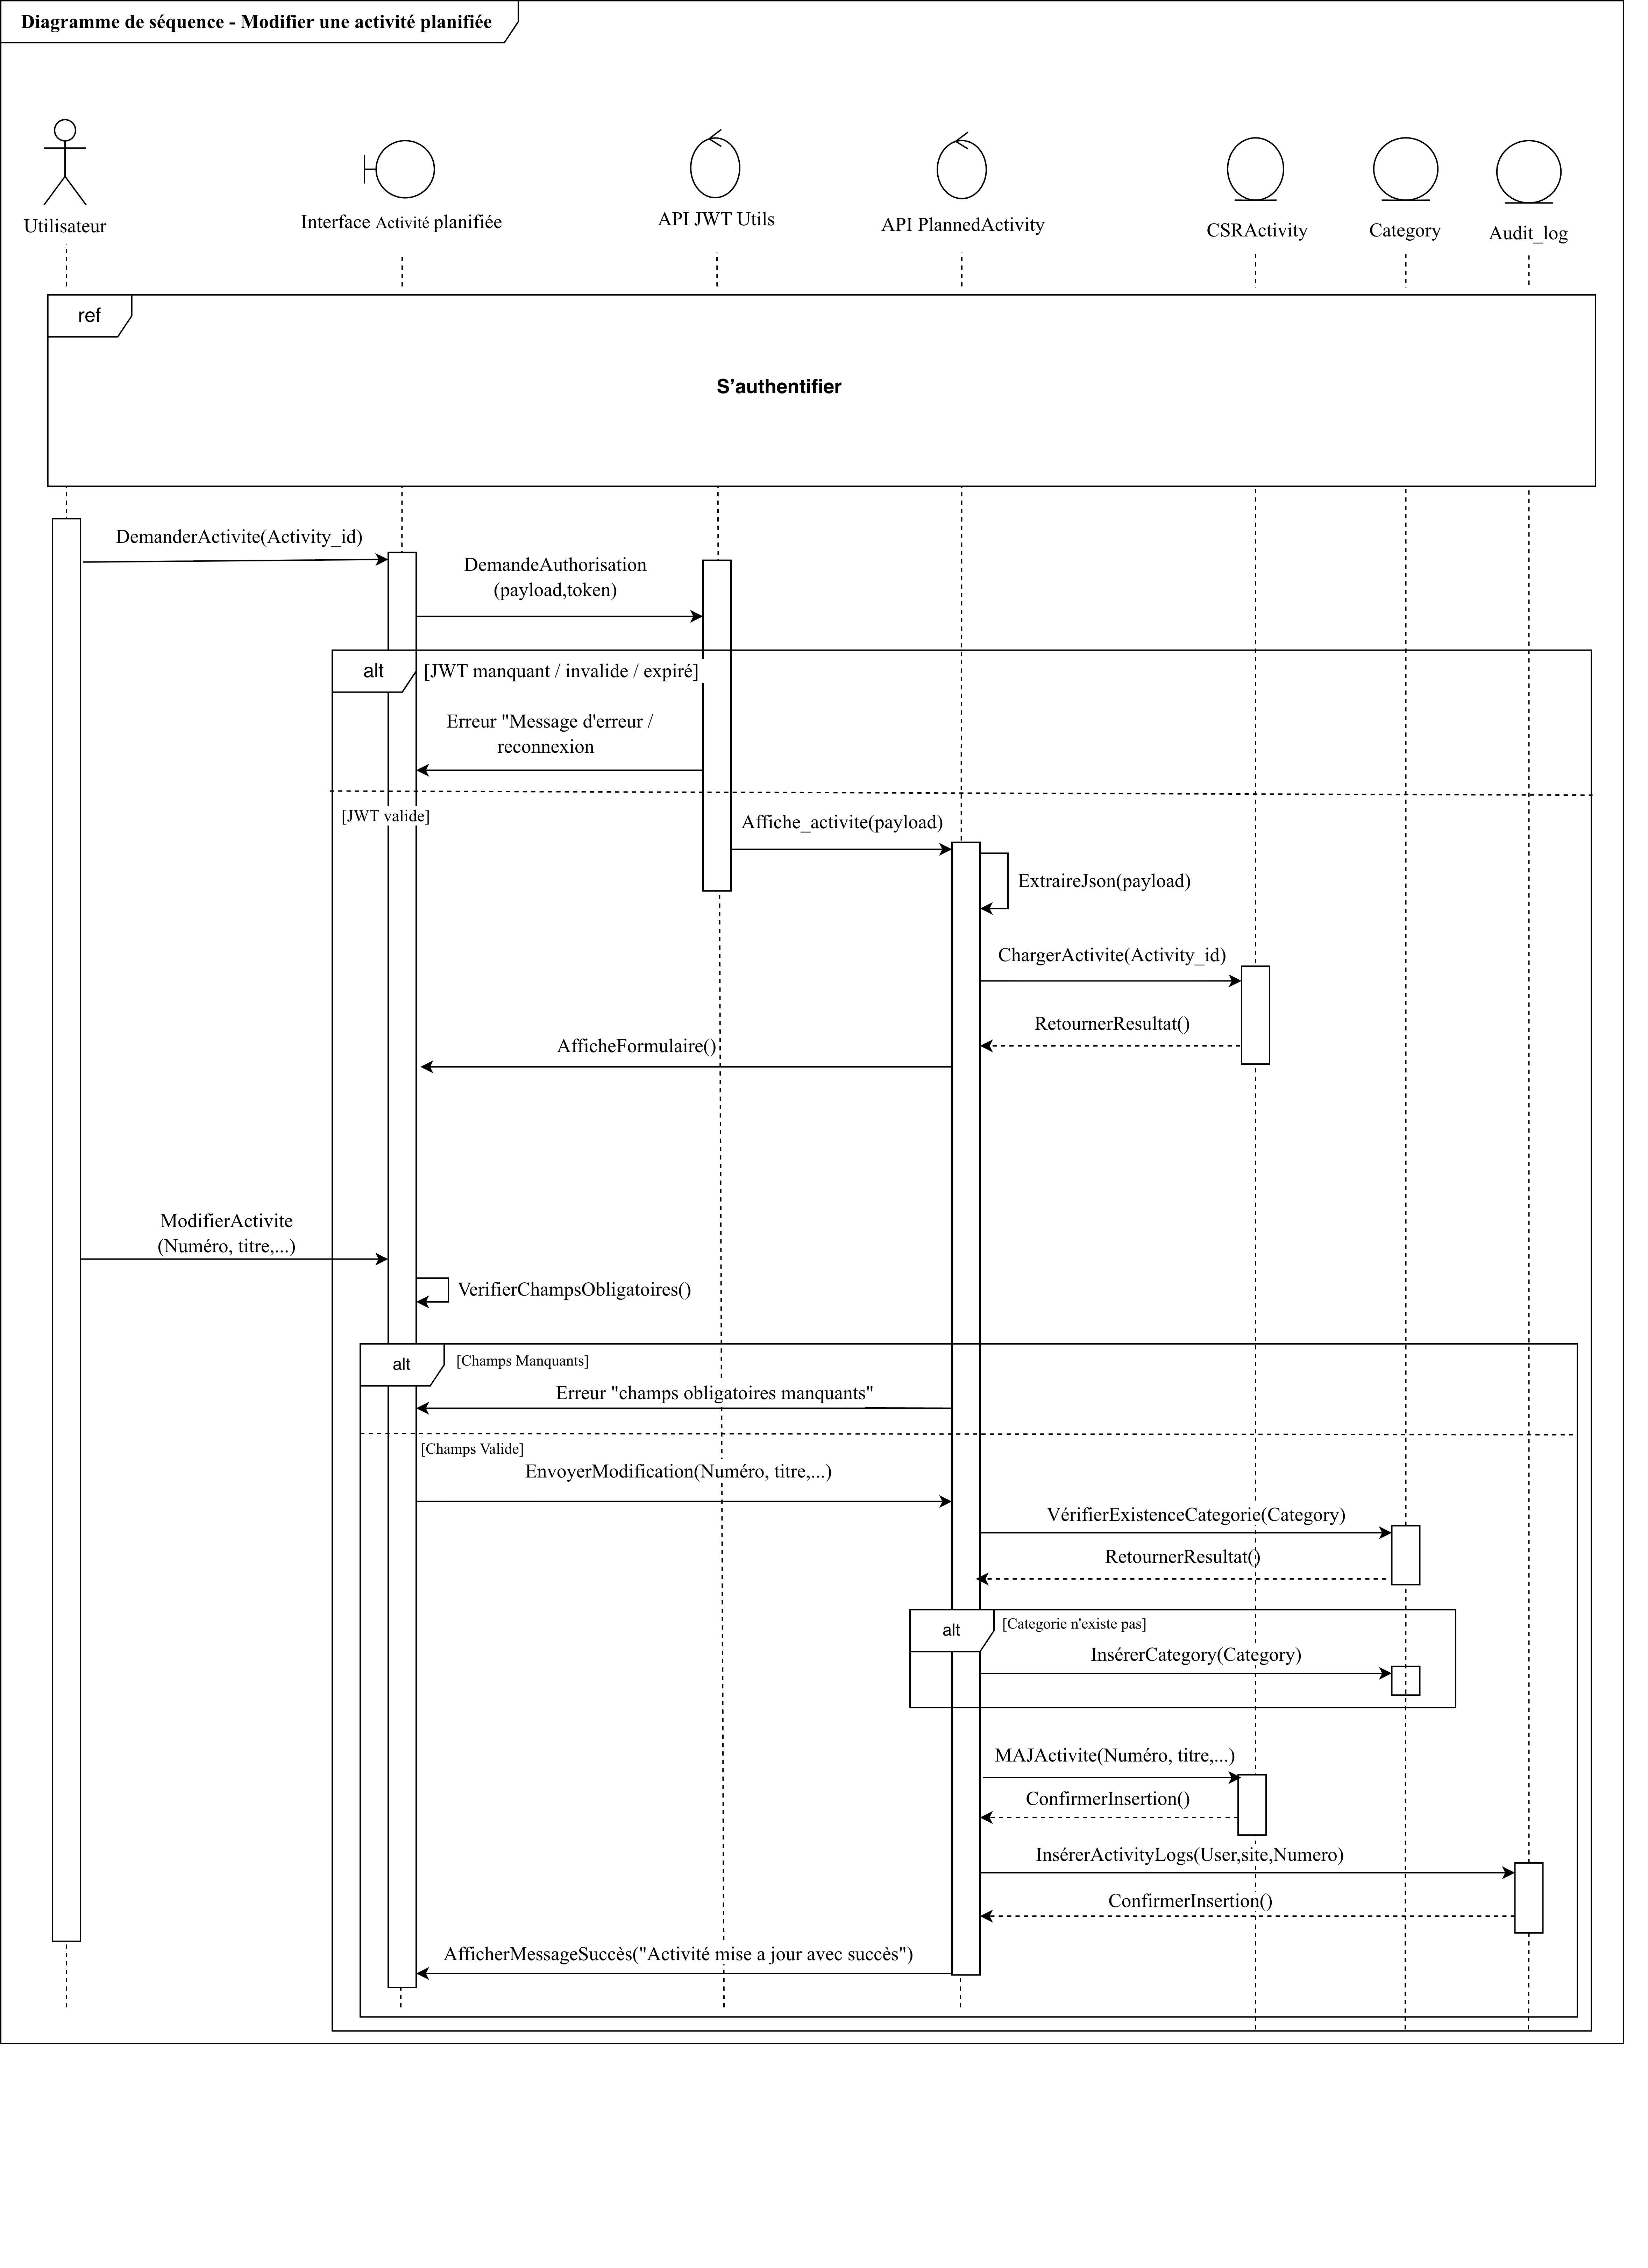
\includegraphics[width=0.92\linewidth]{figures/chapitre-04/diagramme-sequence-modifier-activite-planifiee.png}
  \caption{Diagramme de séquence — «~Modifier une activité planifiée~».}
  \label{fig:doc-ch4-seq-modif-activite}
\end{figure}%

\subsection{Diagramme d’activité}

Les diagrammes d’activité présentent l’enchaînement des traitements et des décisions métier pour les fonctionnalités clés du sprint 2.

\subsubsection{Diagramme d’activité : «~Créer un plan CSR~»}

La figure~\ref{fig:doc-ch4-act-creer-plan} présente le diagramme d’activité du cas «~Créer un plan CSR~».

\begin{figure}[H]
  \centering
  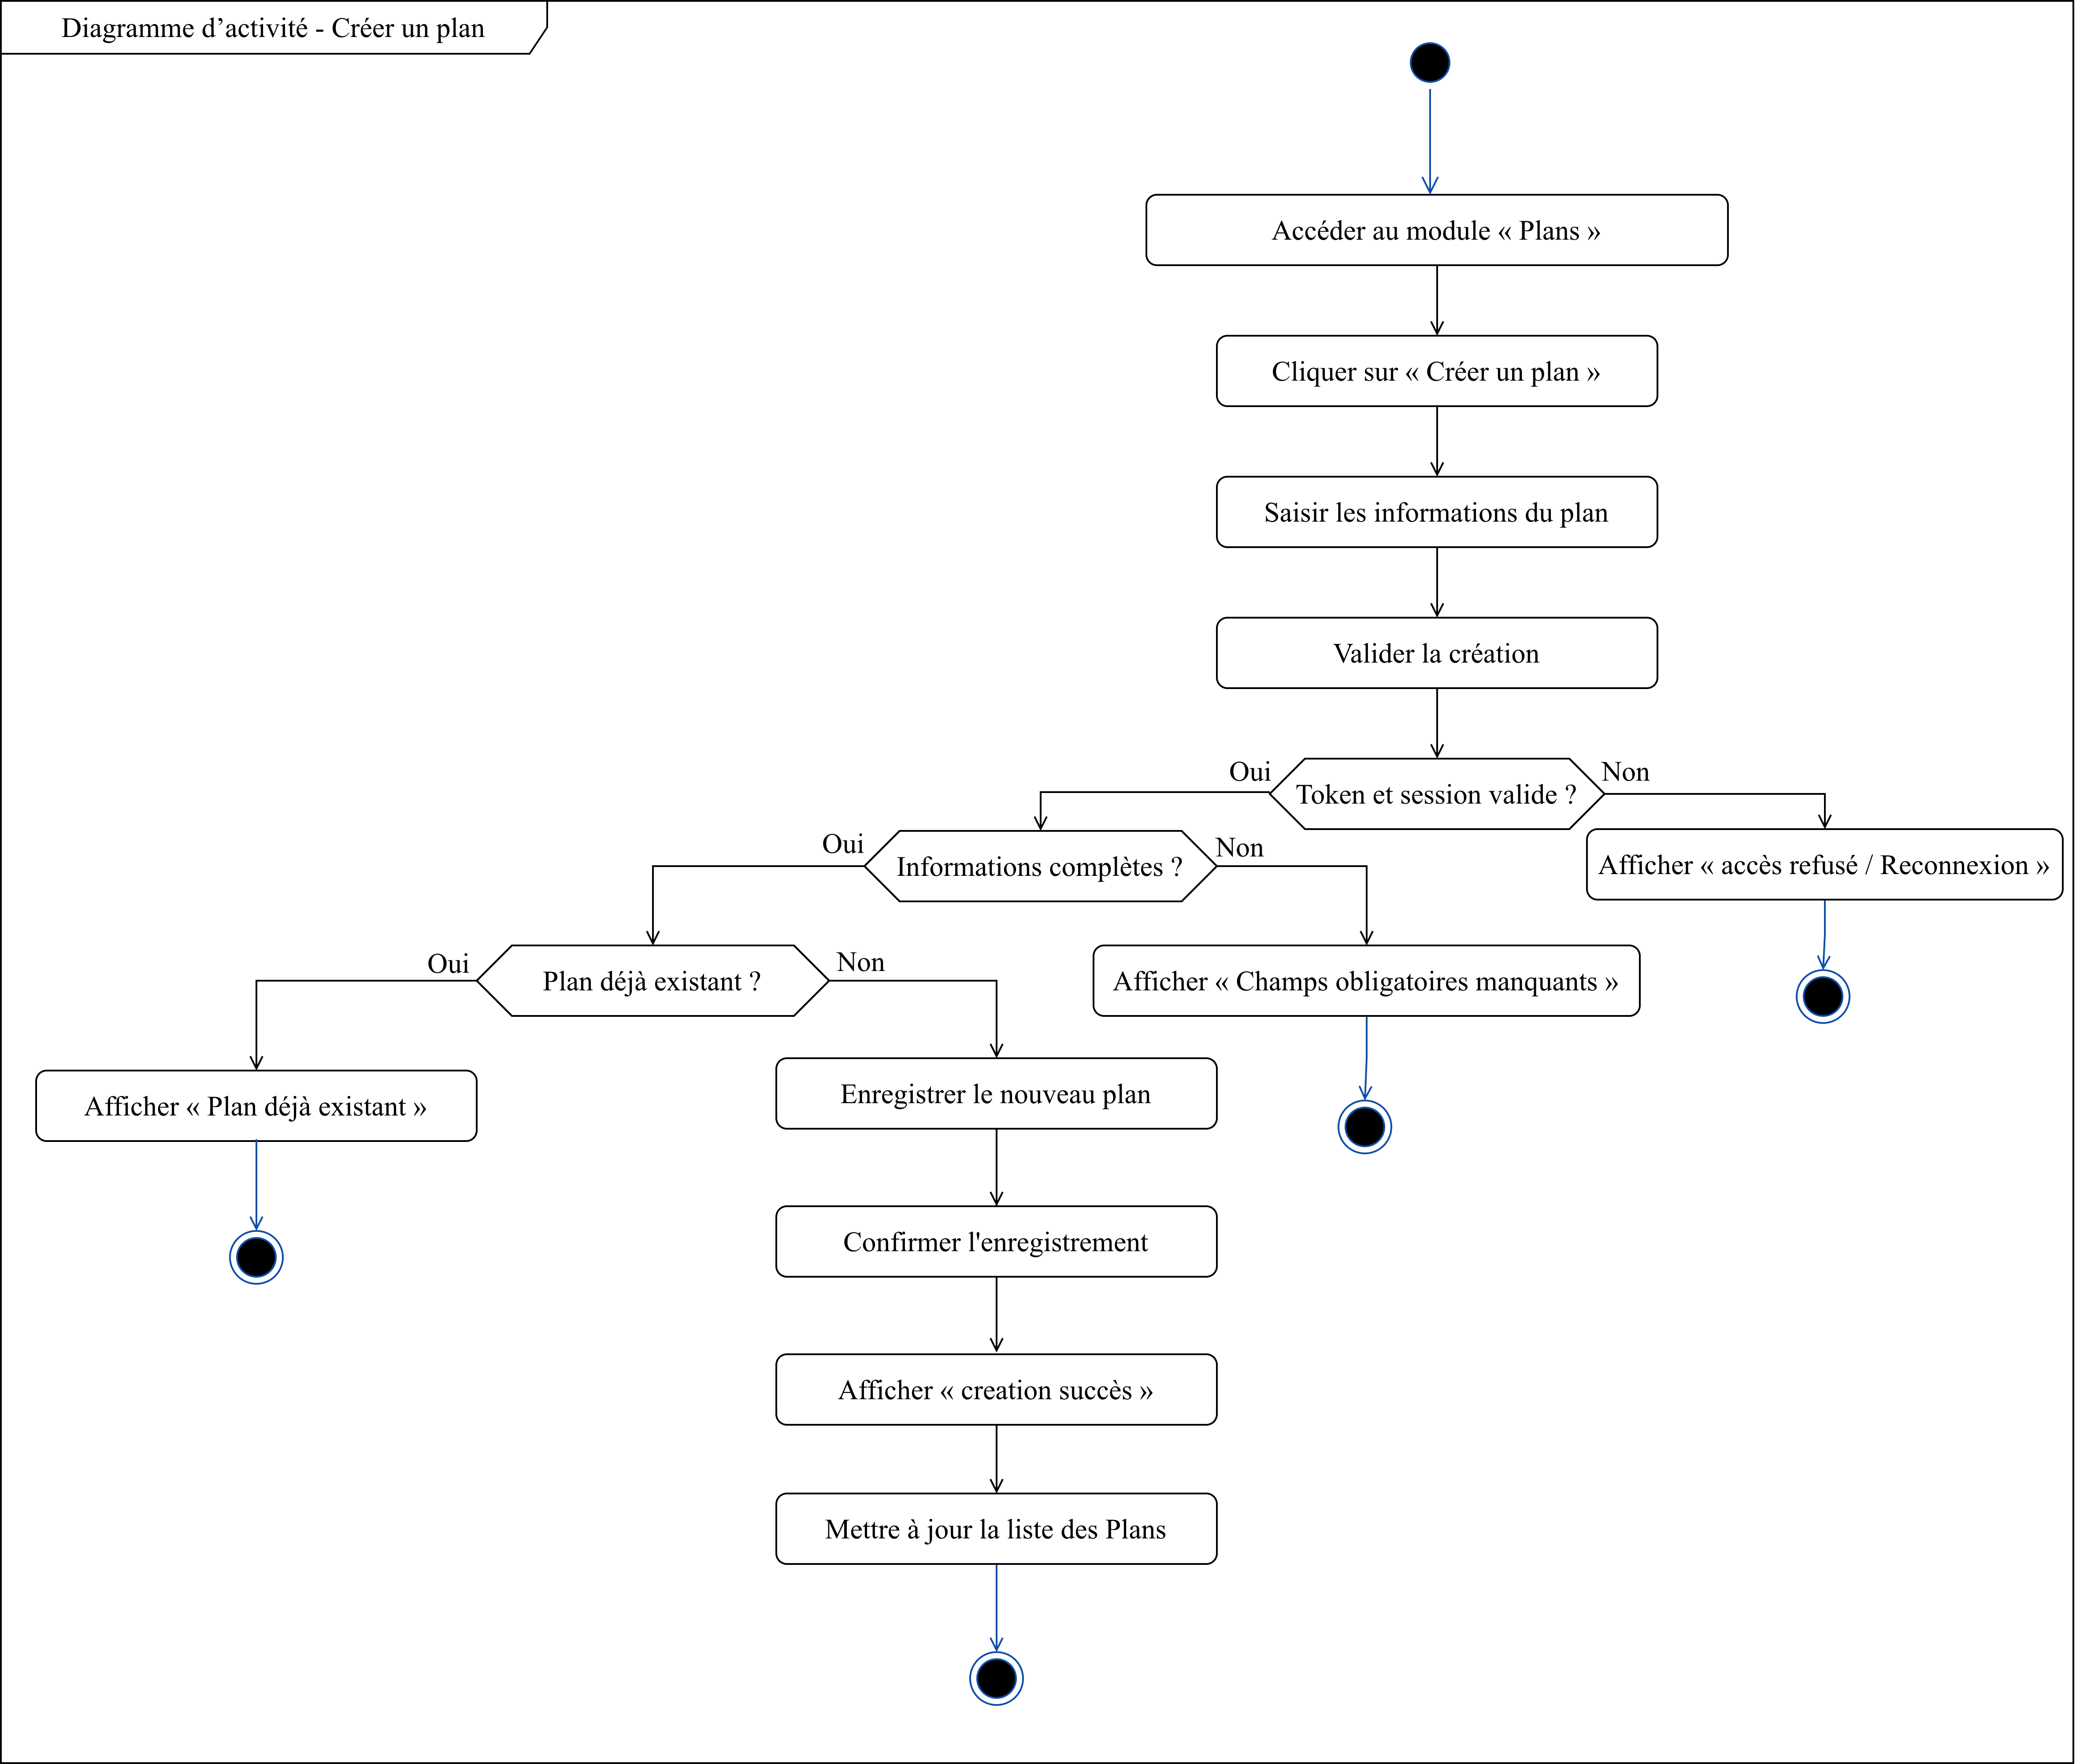
\includegraphics[width=1\linewidth]{figures/chapitre-04/Diagramme_dactivite_cree_un_plan.png}
  \caption{Diagramme d’activité — «~Créer un plan CSR~».}
  \label{fig:doc-ch4-act-creer-plan}
\end{figure}%


\subsubsection{Diagramme d’activité : «~Modifier une activité planifiée~»}

La figure~\ref{fig:doc-ch4-act-modif-activite} présente le diagramme d’activité du cas «~Modifier une activité planifiée~».

\begin{figure}[H]
  \centering
  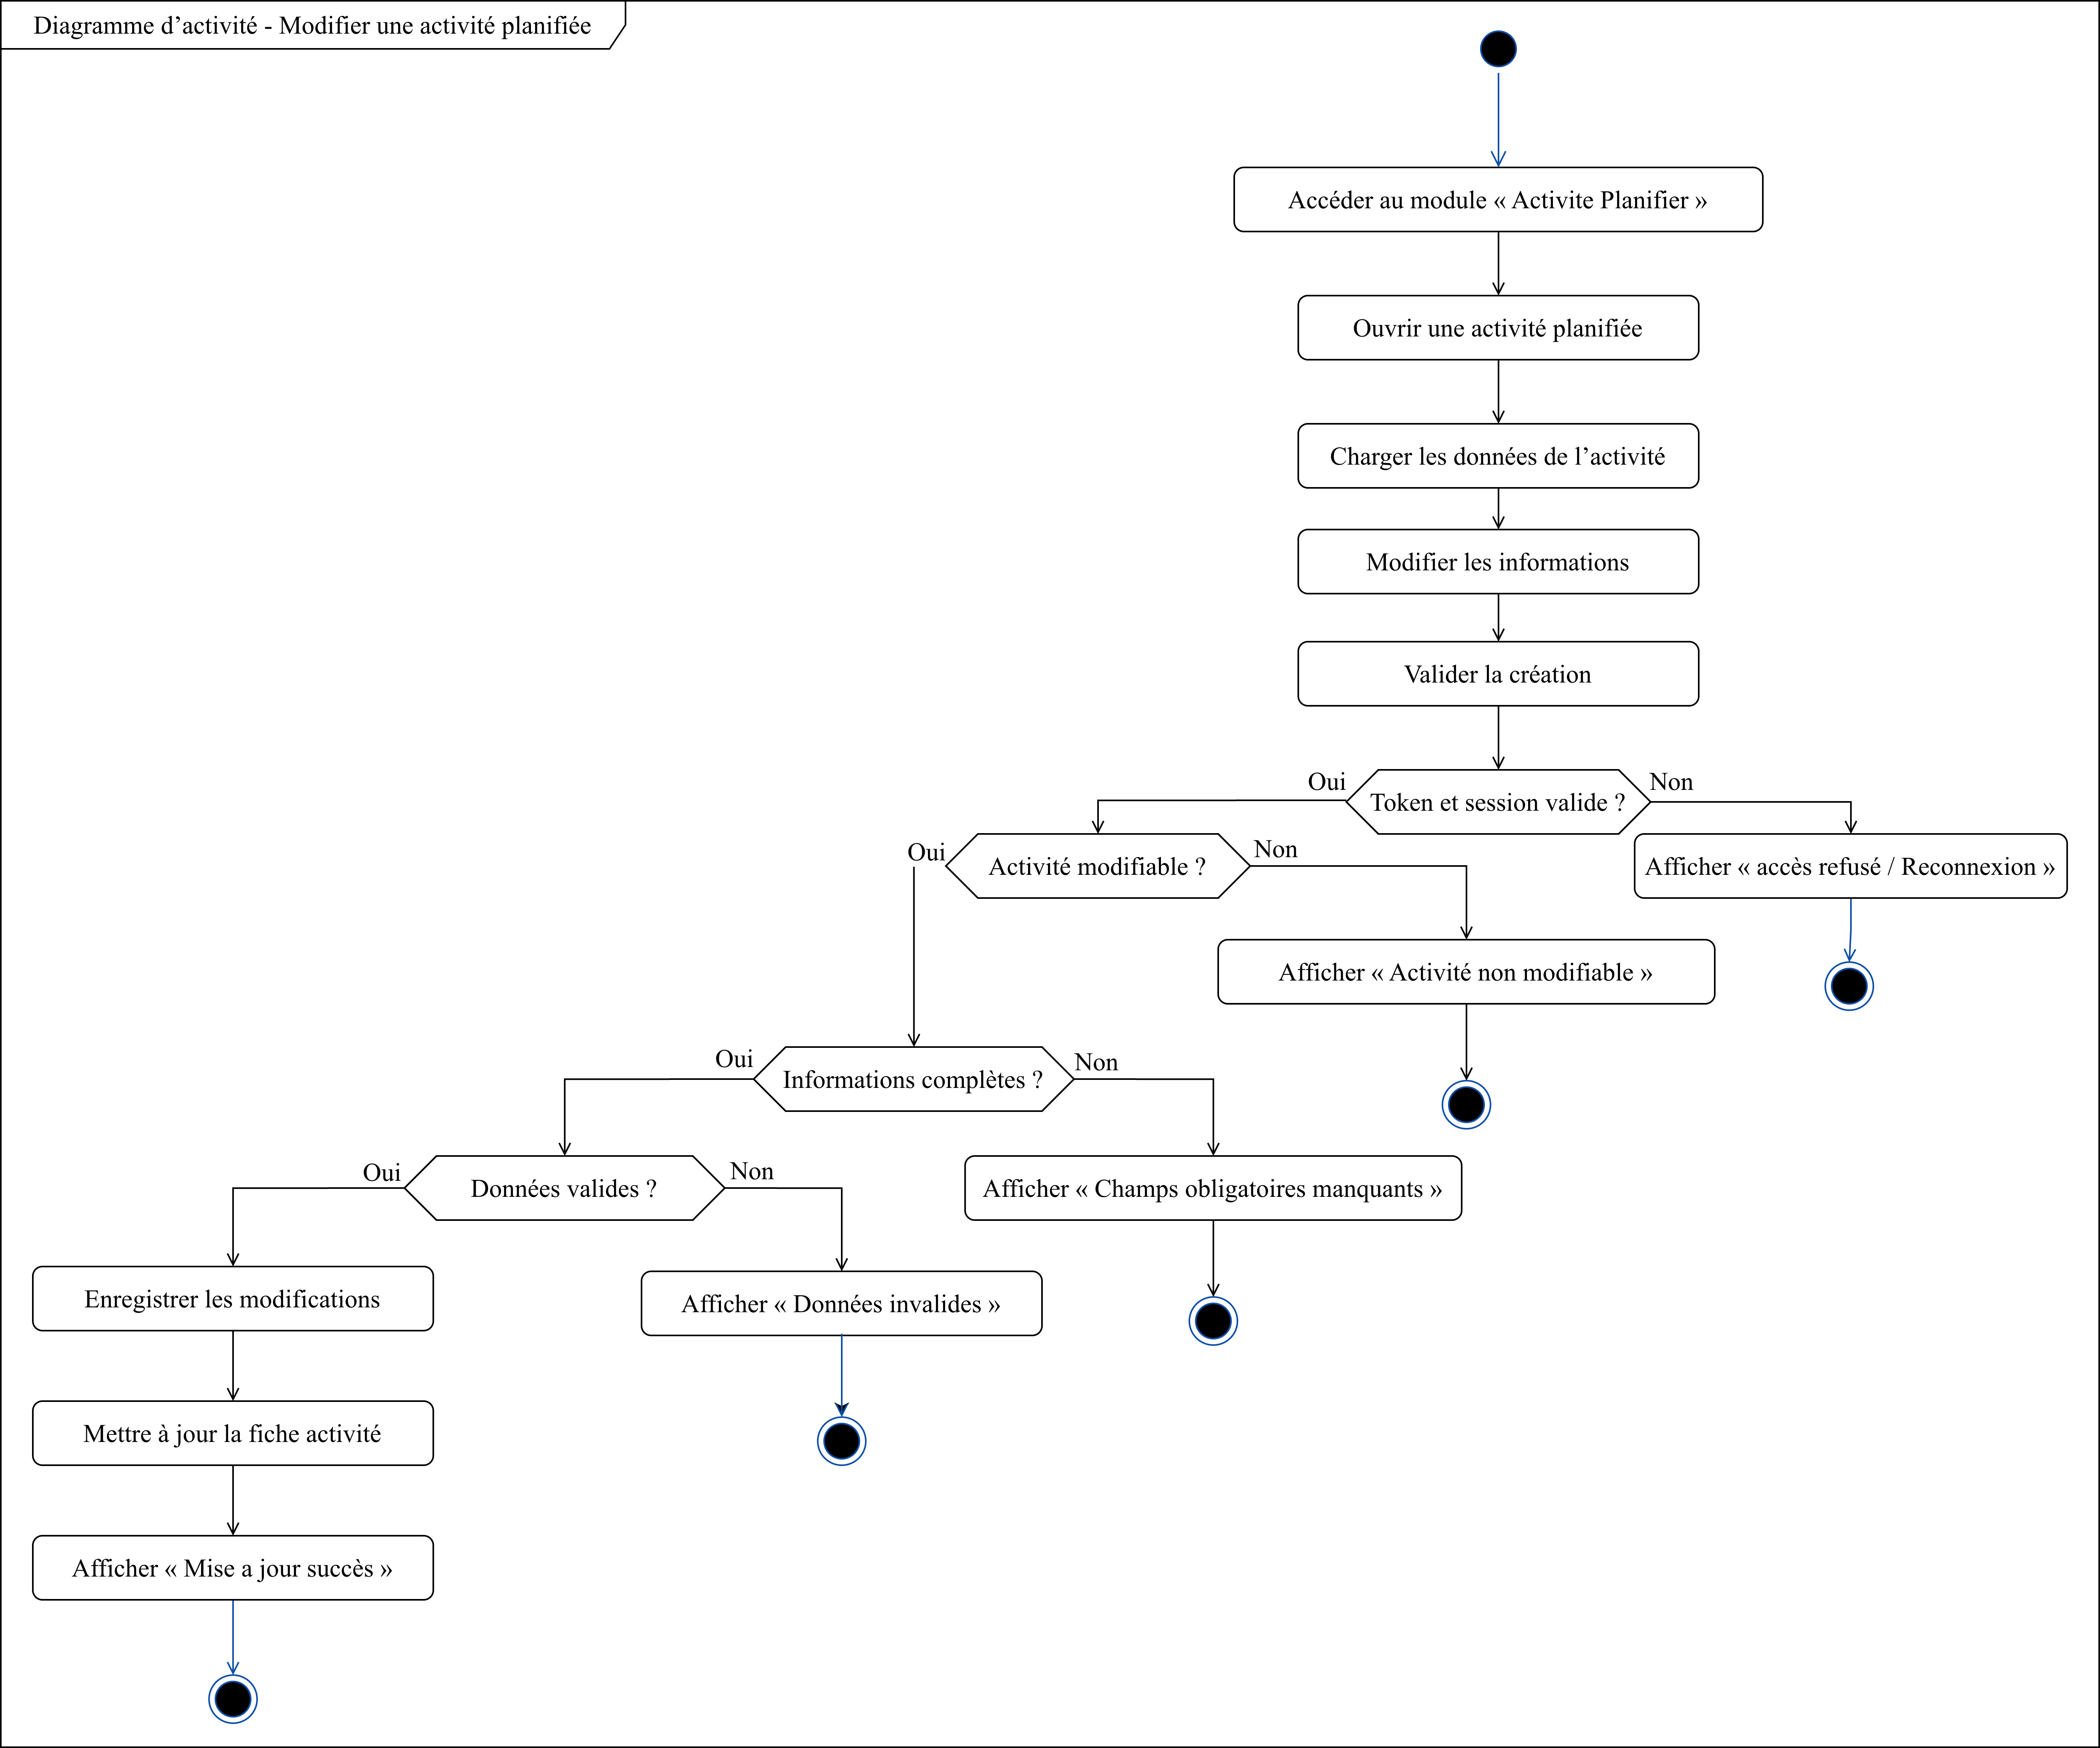
\includegraphics[width=1\linewidth]{figures/chapitre-04/Diagramme_dactivite_modifier_une_activite.png}
  \caption{Diagramme d’activité — «~Modifier une activité planifiée~».}
  \label{fig:doc-ch4-act-modif-activite}
\end{figure}%

\section{Réalisation}

Dans cette section, nous présentons les interfaces réalisées au cours de ce deuxième sprint. Les captures d'écran ci-dessous montrent les principales fonctionnalités développées, notamment la gestion des plans CSR annuels, le suivi des activités planifiées et la saisie des activités réalisées par site. Ces visuels permettent de constater que les fonctionnalités correspondent bien aux besoins définis dans le backlog du sprint.

La figure~\ref{fig:doc-ch4-3} présente la vue liste des plans annuels CSR.

\IfFileExists{figures/chapitre-04/ui-liste-plans-annuels.png}{%
\begin{figure}[H]
  \centering
  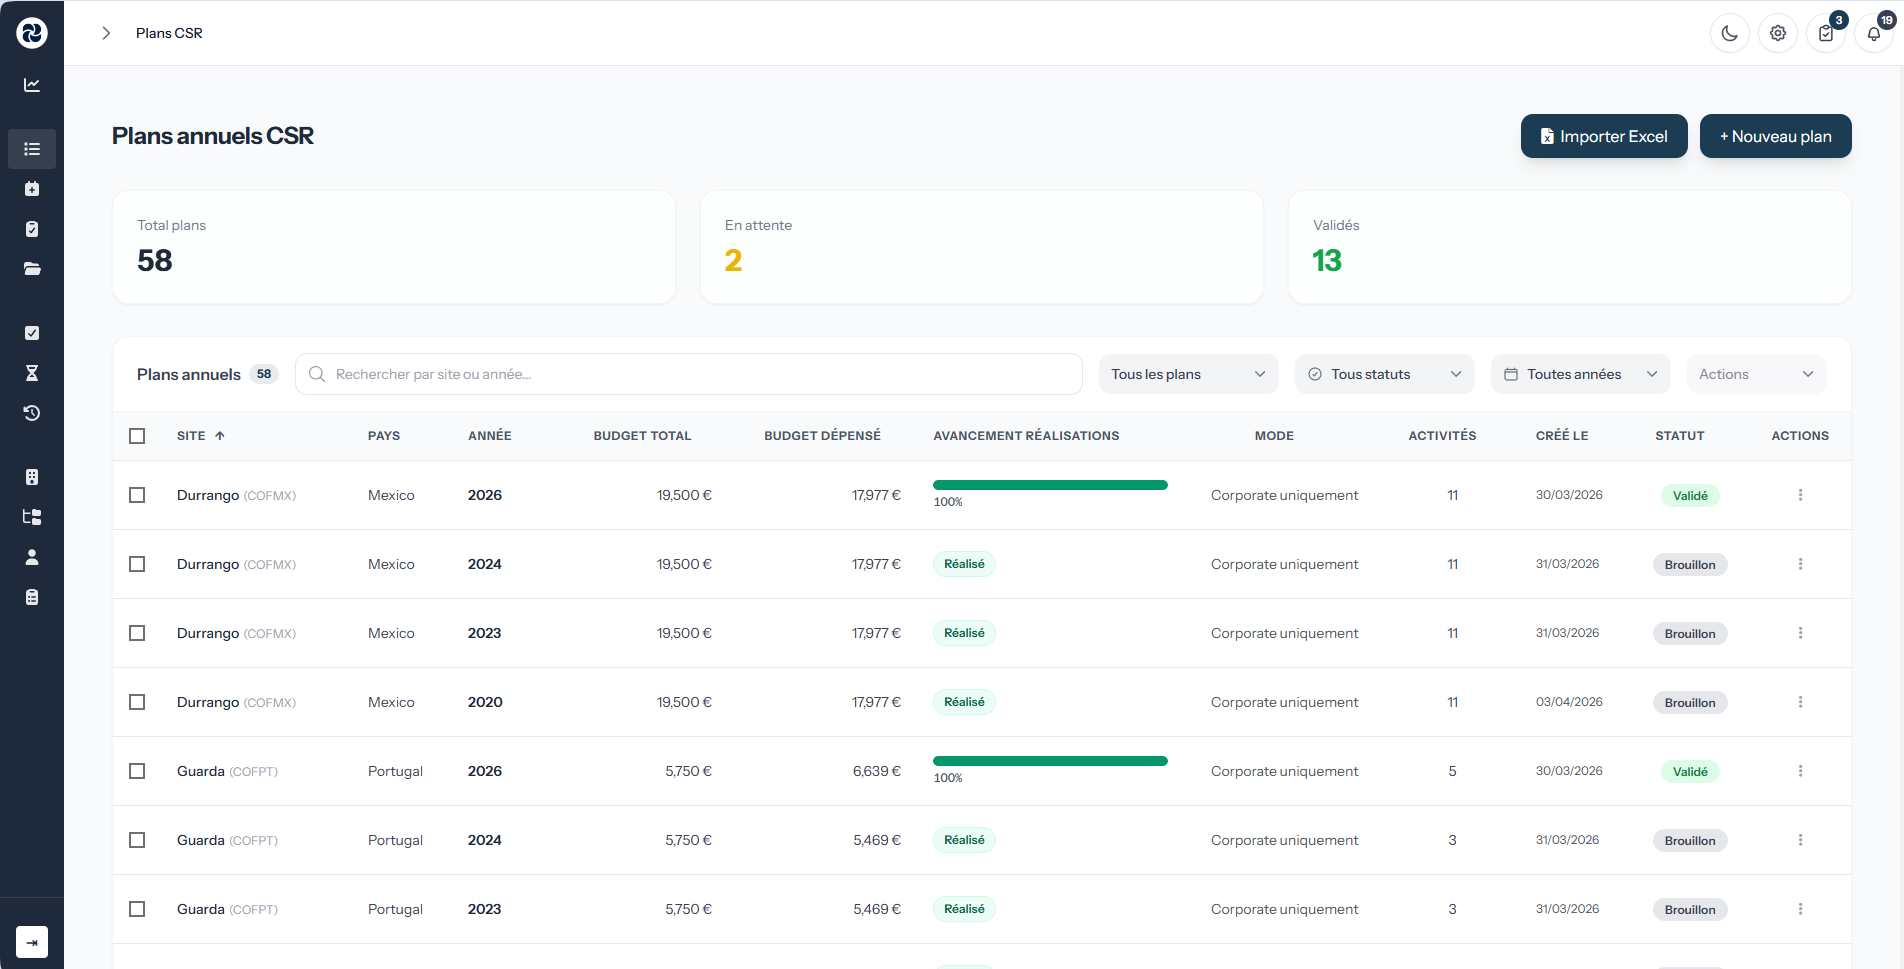
\includegraphics[width=0.92\linewidth]{figures/chapitre-04/ui-liste-plans-annuels.png}
  \caption{Interface : liste des plans annuels CSR.}
  \label{fig:doc-ch4-3}
\end{figure}%
}{%
\begin{figure}[H]
  \centering
  \fbox{\parbox{0.92\linewidth}{\centering\vspace{3.2cm}\textit{(Figure à insérer : \texttt{figures/chapitre-04/ui-liste-plans-annuels.png})}\vspace{3.2cm}}}
  \caption{Interface : liste des plans annuels CSR.}
  \label{fig:doc-ch4-3}
\end{figure}%
}

Cette interface constitue le point d'entrée central du module de planification CSR. Elle offre à l'utilisateur une vue d'ensemble immédiate grâce à trois compteurs affichés en haut de l'écran : le nombre total de plans enregistrés, le nombre de plans en attente de validation et le nombre de plans validés.

Le tableau principal liste les plans par site et par année, en exposant pour chacun le budget total prévu, le budget effectivement dépensé, le taux d'avancement des réalisations sous forme de barre de progression, le mode de validation appliqué, le nombre d'activités rattachées, la date de création ainsi que le statut courant.

Deux actions rapides sont accessibles en haut à droite : la création manuelle d'un nouveau plan et l'import depuis un fichier Excel, couvrant ainsi les deux modes de saisie prévus dans le backlog. Des filtres par site, par statut et par année permettent d'affiner l'affichage selon le besoin de l'utilisateur, qu'il soit responsable d'un seul site ou administrateur corporate supervisant l'ensemble des entités.


\section{Tests et validation}

Les tests occupent une place centrale dans la méthodologie agile, car ils garantissent la qualité ainsi que la fiabilité des fonctionnalités développées. Avant le lancement d’un nouveau sprint, il est indispensable de valider les incréments prioritaires afin de vérifier leur bon fonctionnement et leur conformité aux besoins des parties prenantes.
\subsection{Test}

Dans cette partie, nous présentons une validation fonctionnelle consolidée des fonctionnalités du sprint~2 : gestion des plans CSR, activités planifiées, activités réalisées (y compris hors plan), import Excel et contrôle des doublons.
Le tableau~\ref{tab:ch4-scenarios-tests} synthétise les cas de test correspondants.

% Scénarios de test consolidés — chapitre 4 (plans & activités)
\small
\PFETableSetup
\setlength{\LTpre}{0pt}
\setlength{\LTpost}{0pt}
\setlength{\LTleft}{\fill}
\setlength{\LTright}{\fill}
\setlength{\tabcolsep}{3.5pt}
\renewcommand{\arraystretch}{1.25}

\begin{longtable}{|>{\centering\arraybackslash}m{2.8cm}|
>{\raggedright\arraybackslash}p{2.5cm}|
>{\raggedright\arraybackslash}p{3.8cm}|
>{\raggedright\arraybackslash}p{4.3cm}|
>{\centering\arraybackslash}p{1.1cm}|}
\caption{Synthèse des cas de test du sprint 2}\label{tab:ch4-scenarios-tests}\\
\hline
\tableHeaderStyle
\multicolumn{1}{|c|}{\tableHeaderCell{Nom du cas d'utilisation}} &
\multicolumn{1}{c|}{\tableHeaderCell{Cas de test}} &
\multicolumn{1}{c|}{\tableHeaderCell{Description du cas}} &
\multicolumn{1}{c|}{\tableHeaderCell{Résultat attendu}} &
\multicolumn{1}{c|}{\tableHeaderCell{Résultat réel}} \\
\hline
\endfirsthead
\hline
\multicolumn{5}{|c|}{\tablename\ \thetable{} --- \textit{(suite)}} \\
\hline
\tableHeaderStyle
\multicolumn{1}{|c|}{\tableHeaderCell{Nom du cas d'utilisation}} &
\multicolumn{1}{c|}{\tableHeaderCell{Cas de test}} &
\multicolumn{1}{c|}{\tableHeaderCell{Description du cas}} &
\multicolumn{1}{c|}{\tableHeaderCell{Résultat attendu}} &
\multicolumn{1}{c|}{\tableHeaderCell{Résultat réel}} \\
\hline
\endhead
\hline
\multicolumn{5}{|r|}{\textit{Suite page suivante\ldots}} \\
\hline
\endfoot
\hline
\endlastfoot

\needspace{16\baselineskip}
\multirow{7}{=}{\centering Gérer un plan CSR\\manuellement} &
Créer un plan CSR &
Création d'un nouveau plan annuel avec site, année et budget. &
Le plan est enregistré et visible dans la liste. &
Vrai \\
\cline{2-5}
 &
Consulter un plan CSR &
Ouverture du détail d'un plan déjà créé. &
Les informations du plan sont affichées correctement. &
Vrai \\
\cline{2-5}
 &
Modifier un plan CSR &
Mise à jour des informations d'un plan en état modifiable. &
Les modifications sont enregistrées et visibles. &
Vrai \\
\cline{2-5}
 &
Supprimer un plan CSR &
Suppression d'un plan autorisée selon les règles métier. &
Le plan est supprimé et n'apparaît plus dans la liste. &
Vrai \\
\cline{2-5}
 &
Soumettre un plan CSR pour validation &
Soumission d'un plan complet pour lancer le workflow de validation. &
Le statut passe en « soumis » et le plan devient non modifiable. &
Vrai \\
\cline{2-5}
 &
Importer un plan via Excel &
Import d'un fichier Excel pour créer plan et activités associées. &
Le plan et ses activités sont créés si les données sont valides. &
Vrai \\
\cline{2-5}
 &
Lire et parser le fichier Excel avant l'import &
Vérification de la structure et des données avant confirmation d'import. &
Les erreurs de format sont détectées avant insertion. &
Vrai \\
\hline

\needspace{10\baselineskip}
\multirow{4}{=}{\centering Gérer une activité\\planifiée} &
Créer une activité planifiée &
Ajout d'une nouvelle activité dans un plan CSR. &
L'activité est enregistrée et affichée dans le plan. &
Vrai \\
\cline{2-5}
 &
Consulter une activité planifiée &
Ouverture des détails d'une activité planifiée existante. &
Les informations détaillées sont affichées. &
Vrai \\
\cline{2-5}
 &
Modifier une activité planifiée &
Mise à jour des informations d'une activité planifiée. &
Les modifications sont sauvegardées. &
Vrai \\
\cline{2-5}
 &
Supprimer une activité planifiée &
Suppression d'une activité planifiée selon les règles d'état. &
L'activité est retirée de la liste du plan. &
Vrai \\
\hline

\needspace{10\baselineskip}
\multirow{4}{=}{\centering Gérer une activité\\réalisée} &
Saisir les données réelles de l'activité &
Saisie des données de réalisation (quantités, coûts, période, etc.). &
La réalisation est enregistrée avec succès. &
Vrai \\
\cline{2-5}
 &
Consulter une activité réalisée &
Affichage des détails d'une activité déjà réalisée. &
Les données réelles sont consultables. &
Vrai \\
\cline{2-5}
 &
Modifier une activité réalisée &
Mise à jour des données d'une activité réalisée. &
Les modifications sont enregistrées. &
Vrai \\
\cline{2-5}
 &
Supprimer une activité réalisée &
Suppression d'une réalisation autorisée. &
La réalisation est supprimée de la liste. &
Vrai \\
\hline

\needspace{12\baselineskip}
\multirow{5}{=}{\centering Gérer une activité\\réalisée hors plan} &
Créer une activité réalisée hors plan &
Création d'une activité réalisée non prévue dans le plan initial. &
L'activité hors plan est enregistrée. &
Vrai \\
\cline{2-5}
 &
Consulter une activité réalisée hors plan &
Affichage du détail d'une activité hors plan. &
Les informations sont affichées correctement. &
Vrai \\
\cline{2-5}
 &
Modifier une activité réalisée hors plan &
Mise à jour des informations d'une activité hors plan. &
Les modifications sont sauvegardées. &
Vrai \\
\cline{2-5}
 &
Supprimer une activité réalisée hors plan &
Suppression d'une activité hors plan existante. &
L'activité est supprimée de la liste. &
Vrai \\
\cline{2-5}
 &
Soumettre une activité réalisée hors plan pour validation &
Envoi de l'activité hors plan dans le circuit de validation. &
Le statut passe en attente de validation. &
Vrai \\
\hline

\needspace{7\baselineskip}
\multirow{2}{=}{\centering Contrôler les\\duplicatas (import Excel)} &
Supprimer les duplicatas &
Suppression des lignes dupliquées avant import. &
Les doublons sont retirés du jeu de données. &
Vrai \\
\cline{2-5}
 &
Ignorer les duplicatas et continuer &
Poursuite de l'import en ignorant les lignes dupliquées détectées. &
L'import continue sans bloquer sur les doublons. &
Vrai \\
\hline

\end{longtable}
\normalsize


\newpage

Les figures~\ref{fig:ch4-postman-plans} sont prévues pour les captures correspondantes.

\begin{figure}[H]
  \centering
  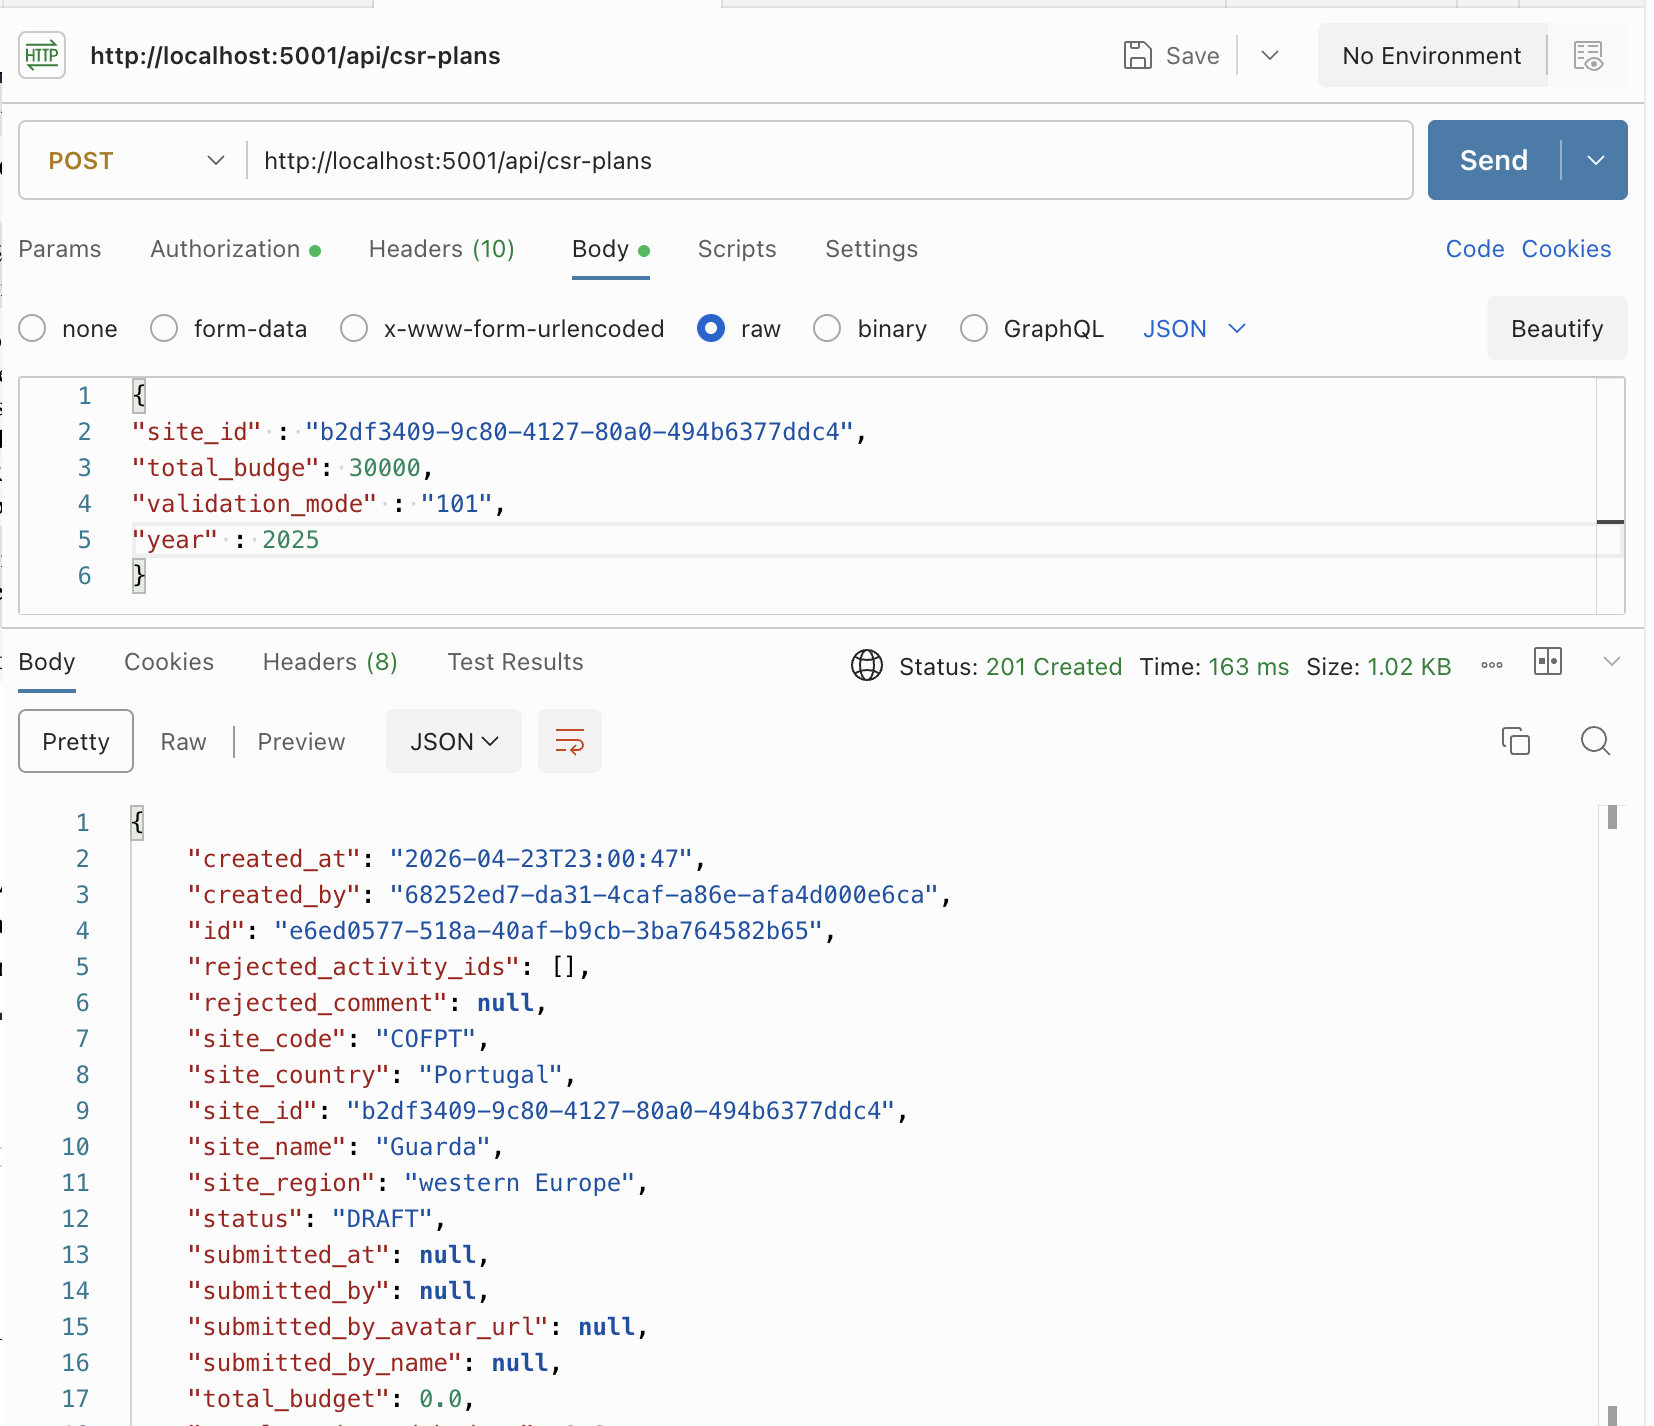
\includegraphics[width=0.92\linewidth]{figures/chapitre-04/postman-csr-plans.png}
  \caption{Tests Postman — création de plan.}
  \label{fig:ch4-postman-plans}
\end{figure}

\subsection{Validation}

Une revue de fin de sprint avec le \emph{Scrum Master} et le \emph{Product Owner} a permis de valider les parcours plans et activités CSR (création, importation, modification, suppression). Les correctifs mineurs d'ergonomie et de messages utilisateur ont été intégrés avant la bascule vers le sprint suivant centré sur les workflows transverses.

\section{Conclusion}

Ce sprint enrichit la plateforme en couvrant le cœur métier de la planification CSR par site et en préparant le terrain pour le suivi de l'exécution.

Il ouvre la voie au sprint suivant, dédié aux workflows transverses (validations croisées, demandes de modification, notifications et traçabilité).



% Sprint 3 — planification ch. 2 : workflow transverse (demandes, notifications, tâches, audit, chatbot)
\PFEChapterOpening{Sprint 3 - Gestion transverse des validations, notifications et traçabilité}

\section{Introduction}

Ce troisième sprint couvre les besoins transverses qui assurent la gouvernance globale de la plateforme CSR:
la soumission et le traitement des demandes de modification, la validation des plans, les notifications,
la gestion des tâches et la traçabilité des actions.

L'objectif est de fiabiliser le cycle de vie des données déjà saisies, en offrant un cadre de contrôle
cohérent entre les utilisateurs Site et Corporate.

\section{Objectif attendu}

Ce troisième sprint a pour objectif d'introduire un mécanisme de gestion globale au sein de la plateforme CSR, en structurant le cycle de validation des plans et des activités.
Il vise à encadrer les différentes étapes du cycle de validation, depuis la soumission jusqu'à la validation ou le rejet, tout en garantissant le respect des règles métier et des niveaux d'approbation définis.

Ce sprint met également en place un système de traçabilité permettant de conserver l'historique des actions effectuées, ainsi qu'un module de gestion des demandes de modification pour encadrer les ajustements après validation.
Par ailleurs, il intègre des fonctionnalités de notification et de gestion des tâches afin d'assurer une meilleure coordination entre les acteurs et un suivi efficace des actions à réaliser.

L'ensemble de ces éléments contribue à renforcer le contrôle, la transparence et la fiabilité des données, tout en assurant une gestion structurée et collaborative des processus CSR.

\section{Sprint Backlog}

Le Sprint Backlog regroupe l'ensemble des fonctionnalités retenues depuis le Product Backlog pour être développées au cours de ce sprint. Il constitue une vision détaillée et opérationnelle du travail à accomplir, en décomposant chaque fonctionnalité en tâches concrètes et réalisables.

Le tableau~\ref{tab:sprint-backlog-3} présente le backlog du troisième sprint.

% --- Sprint backlog — Workflow transverse (issu du Tableau 5.1 du brouillon Word) ---
\small
\PFETableSetup

\setlength{\PFEbacklogTabW}{\dimexpr\textwidth+2.8cm\relax}
\setlength{\LTcapwidth}{\PFEbacklogTabW}
\setlength{\LTleft}{\fill}
\setlength{\LTright}{\fill}

\setlength{\LTpre}{0pt}
\setlength{\LTpost}{0pt}

\PFETableArrayStretch
\setlength{\extrarowheight}{4pt}
\renewcommand{\arraystretch}{1.4}

\arrayrulecolor{black}

\begin{longtable}{|>{\centering\arraybackslash}m{1.2cm}|>{\raggedright\arraybackslash}m{5.2cm}|>{\centering\arraybackslash}m{1.6cm}|>{\raggedright\arraybackslash}m{5.5cm}|>{\centering\arraybackslash}m{1.7cm}|}

\caption{Sprint backlog du sprint 3 — Gestion transverse des validations, notifications et traçabilité}\label{tab:sprint-backlog-3}\\

\hline
\tableHeaderStyle
\tableHeaderCell{ID} & \tableHeaderCell{User story} & \tableHeaderCell{Tâche ID} & \tableHeaderCell{Tâche} & \tableHeaderCell{Priorité} \\
\hline
\endfirsthead

\hline
\multicolumn{5}{|c|}{\tablename\ \thetable{} — \textit{(suite)}} \\
\hline
\tableHeaderStyle
\tableHeaderCell{ID} & \tableHeaderCell{User story} & \tableHeaderCell{Tâche ID} & \tableHeaderCell{Tâche} & \tableHeaderCell{Priorité} \\
\hline
\endhead

\hline
\multicolumn{5}{|r|}{\textit{Suite page suivante\ldots}} \\
\hline
\endfoot

\hline
\endlastfoot

1 & En tant qu'utilisateur, je veux soumettre une entité (plan ou activité) afin de déclencher le processus de validation & 1.1 &
Implémenter le mécanisme de soumission (plan / activité) & +++++ \\
\cline{3-5}
& & 1.2 &
Vérifier la complétude des données avant soumission & +++++ \\
\cline{3-5}
& & 1.3 &
Changer le statut (DRAFT $\rightarrow$ SUBMITTED) & +++++ \\
\cline{3-5}
& & 1.4 &
Enregistrer la date et l'utilisateur de soumission & ++++ \\
\cline{3-5}
& & 1.5 &
Verrouiller l'entité après soumission & ++++ \\
\hline
2 & En tant qu'utilisateur Corporate, je veux valider une entité afin de confirmer sa conformité & 2.1 &
Implémenter la validation des plans et activités & +++++ \\
\cline{3-5}
& & 2.2 &
Mettre à jour le statut (Under Review $\rightarrow$ Approved) & +++++ \\
\cline{3-5}
& & 2.3 &
Enregistrer les informations de validation (date, acteur) & +++++ \\
\cline{3-5}
& & 2.4 &
Permettre la validation multi-niveaux si nécessaire & ++++ \\
\cline{3-5}
& & 2.5 &
Verrouiller l'entité validée & ++++ \\
\hline
3 & En tant qu'utilisateur Corporate, je veux rejeter une entité afin de demander une correction & 3.1 &
Implémenter le rejet des plans et activités & +++++ \\
\cline{3-5}
& & 3.2 &
Ajouter un champ commentaire obligatoire & +++++ \\
\cline{3-5}
& & 3.3 &
Mettre à jour le statut (Under Review $\rightarrow$ Rejected) & +++++ \\
\cline{3-5}
& & 3.4 &
Rendre l'entité modifiable après rejet & +++++ \\
\hline
4 & En tant qu'utilisateur Site, je veux soumettre une demande de modification afin de corriger des données verrouillées & 4.1 &
Implémenter le module de demandes de modification & +++++ \\
\cline{3-5}
& & 4.2 &
Permettre la création d'une demande avec justification et la durée & +++++ \\
\cline{3-5}
& & 4.3 &
Ajouter la gestion des pièces jointes & ++++ \\
\cline{3-5}
& & 4.4 &
Associer la demande à une entité (plan / activité) & +++++ \\
\cline{3-5}
& & 4.5 &
Définir le statut de la demande (En Attente, Approuvée, Rejetée) & ++++ \\
\hline
5 & En tant qu'utilisateur Corporate, je veux traiter les demandes de modification afin de garder le contrôle & 5.1 &
Consulter les demandes de modification & +++++ \\
\cline{3-5}
& & 5.2 &
Approuver une demande de modification & +++++ \\
\cline{3-5}
& & 5.3 &
Rejeter une demande avec justification & ++++ \\
\cline{3-5}
& & 5.4 &
Déverrouiller temporairement l'entité après approbation & ++++ \\
\hline
6 & En tant qu'utilisateur, je veux recevoir des notifications afin d'être informé des actions du système & 6.1 &
Implémenter le module de notifications & +++++ \\
\cline{3-5}
& & 6.2 &
Envoyer une notification lors de la soumission & +++++ \\
\cline{3-5}
& & 6.3 &
Envoyer une notification lors de validation & +++++ \\
\cline{3-5}
& & 6.4 &
Envoyer une notification lors de rejet & +++++ \\
\cline{3-5}
& & 6.5 &
Notifier les demandes de modification & +++++ \\
\cline{3-5}
& & 6.6 &
Permettre la consultation des notifications & ++++ \\
\hline
7 & En tant qu'utilisateur, je veux gérer mes tâches afin de suivre les actions à effectuer & 7.1 &
Implémenter le module de gestion des tâches & +++++ \\
\cline{3-5}
& & 7.2 &
Générer automatiquement une tâche après soumission & +++++ \\
\cline{3-5}
& & 7.3 &
Assigner les tâches aux utilisateurs concernés & +++++ \\
\cline{3-5}
& & 7.4 &
Permettre la consultation des tâches & ++++ \\
\hline
8 & En tant qu'utilisateur Corporate , je veux tracer toutes les actions afin d'assurer la traçabilité du système & 8.1 &
Implémenter le module d'audit & +++++ \\
\cline{3-5}
& & 8.2 &
Enregistrer chaque action (création, modification, validation\ldots) & +++++ \\
\cline{3-5}
& & 8.3 &
Associer chaque action à un utilisateur & +++++ \\
\cline{3-5}
& & 8.4 &
Enregistrer la date et le type d'action & +++++ \\
\cline{3-5}
& & 8.5 &
Permettre la consultation de l'historique & ++++ \\
\cline{3-5}
& & 8.6 &
Filtrer l'historique (par entité, action, site) & ++++ \\
\hline

\end{longtable}

\normalsize

\newpage
\section{Analyse détaillée des besoins}

\subsection{Diagramme de cas d'utilisation}

La figure~\ref{fig:doc-ch5-1} regroupe les cas d'utilisation du sprint 3 : Gestion transverse des validations, notifications et traçabilité.

\begin{figure}[H]
  \centering
  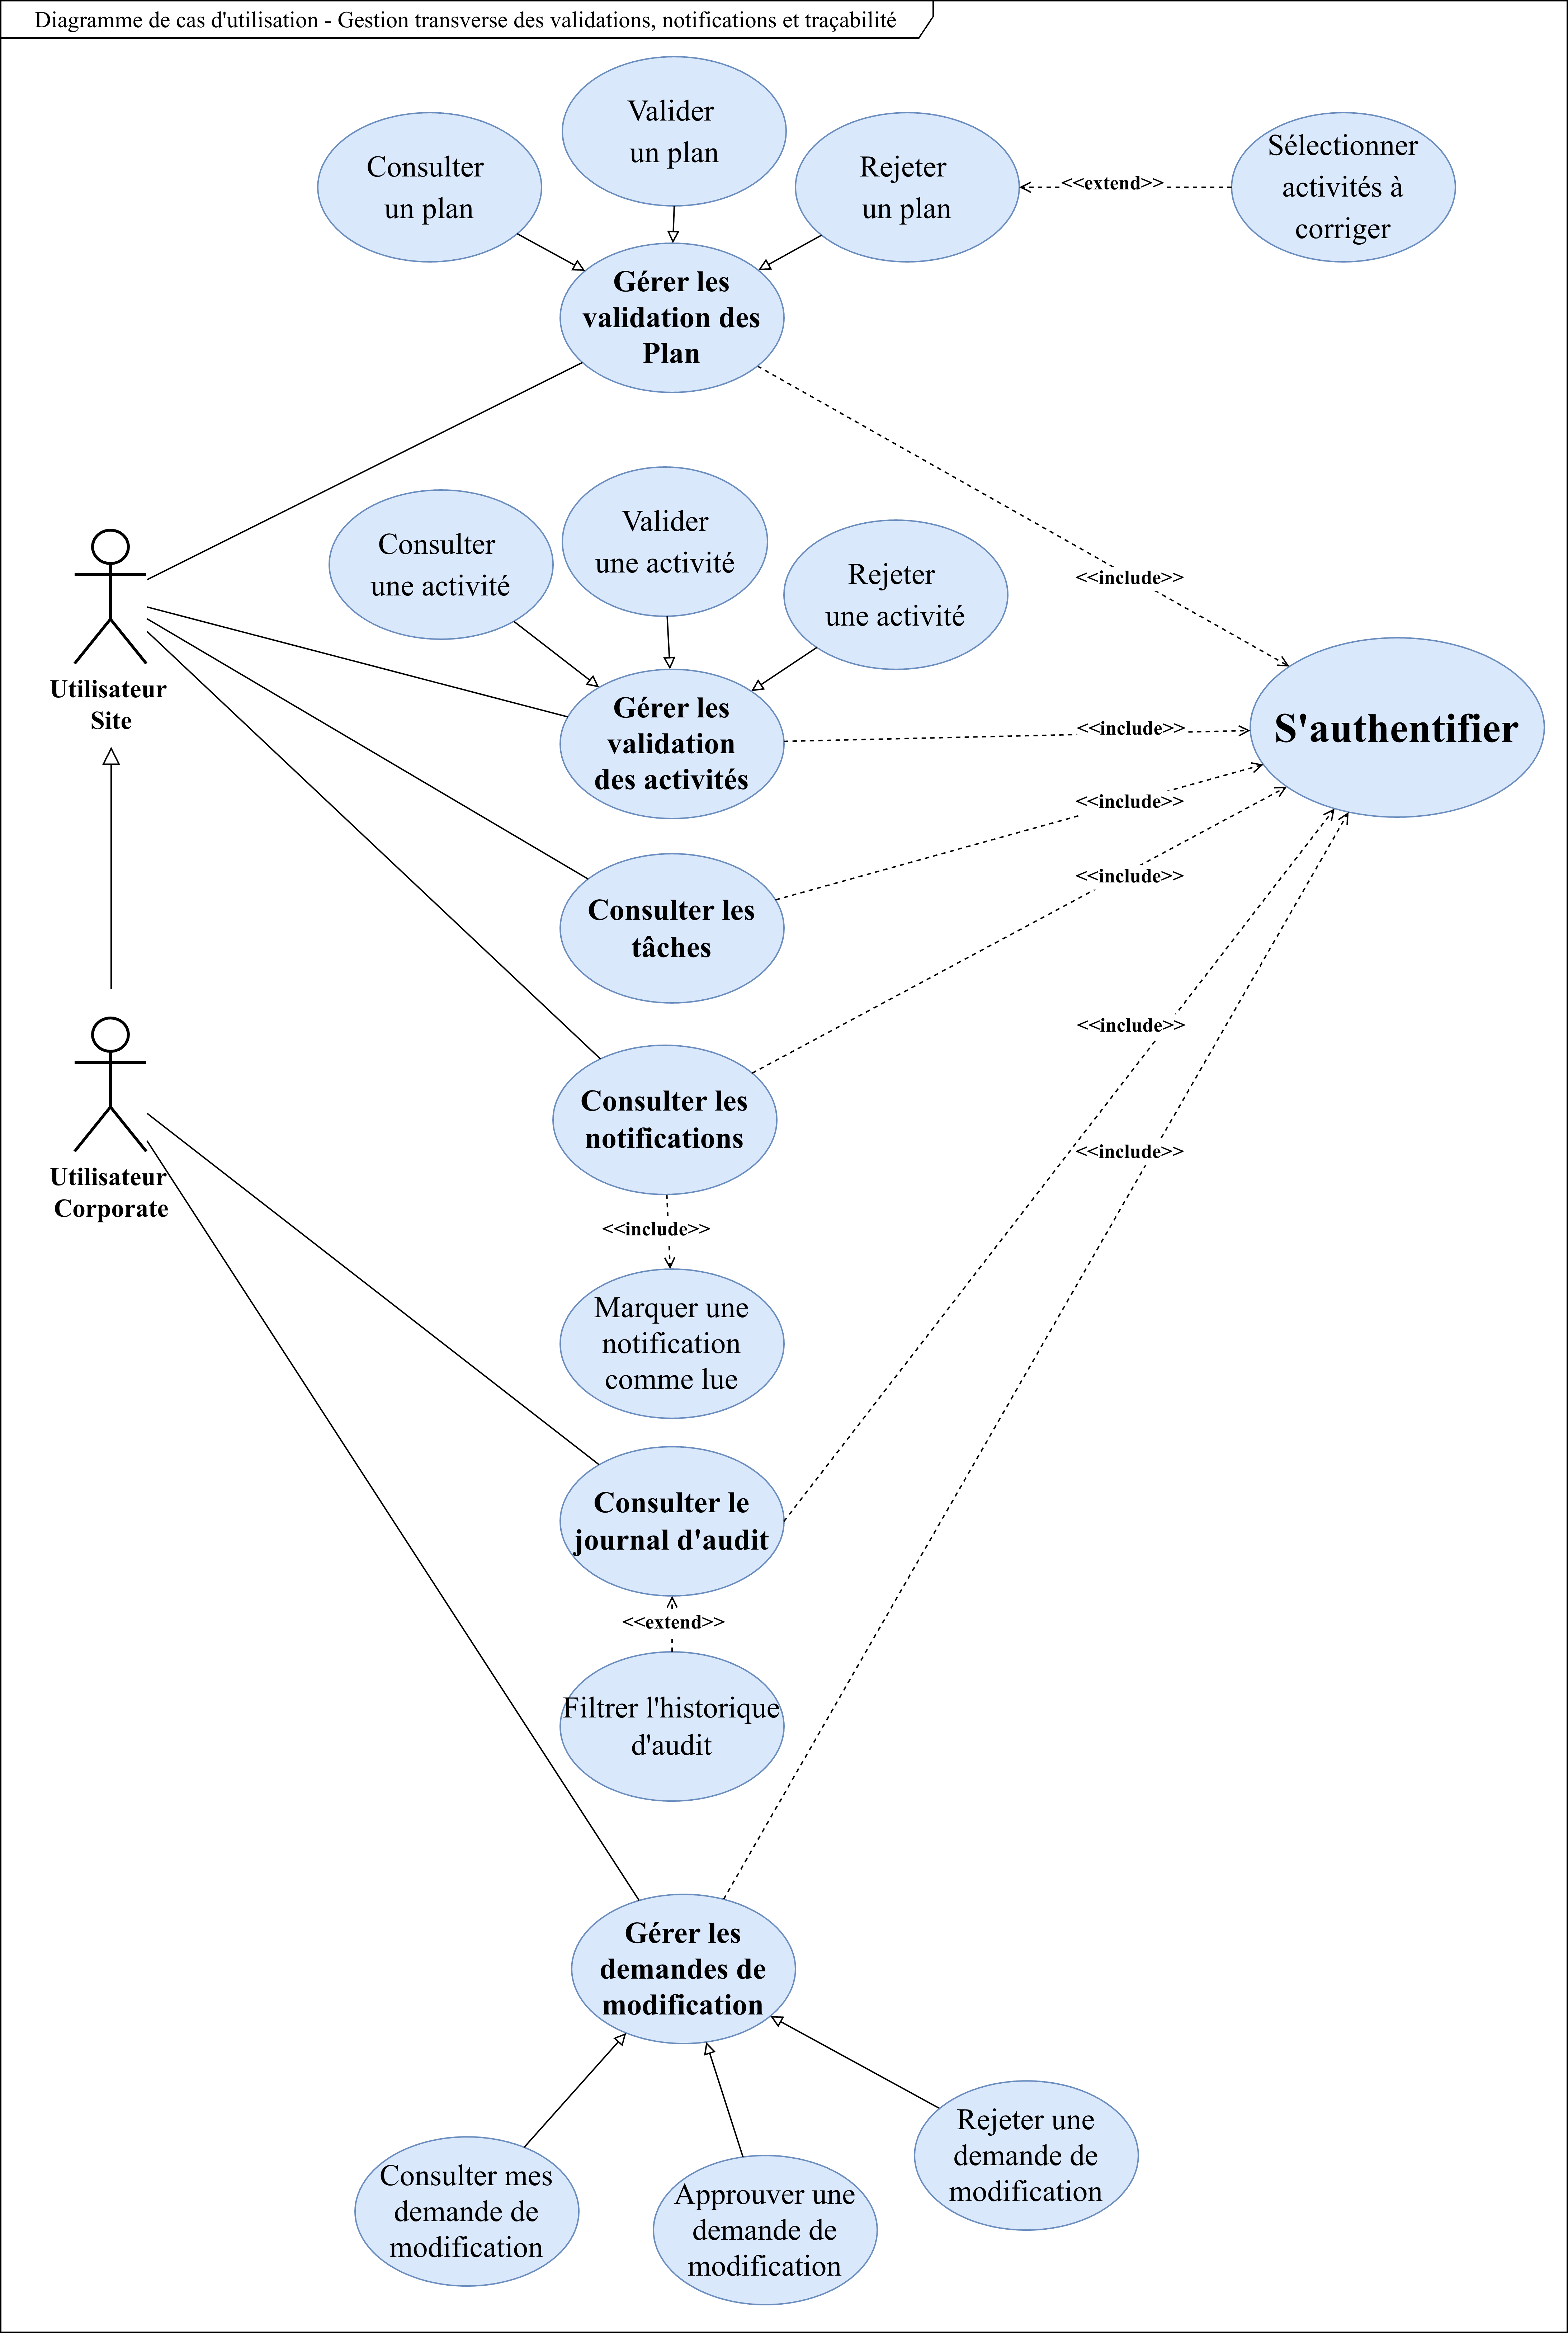
\includegraphics[width=0.85\linewidth]{figures/chapitre-05/diagramme-cas-utilisation-workflow-transverse.png}
  \caption{Diagramme de cas d'utilisation — Gestion transverse des validations, notifications et traçabilité.}
  \label{fig:doc-ch5-1}
\end{figure}%


\subsection{Description textuelle du cas d'utilisation : «~Soumettre une demande de modification pour un plan~»}

Le tableau~\ref{tab:cu-soumettre-demande-modification} expose la description textuelle du cas d'utilisation «~Soumettre une demande de modification pour un plan~».

\begin{table}[H]
  \centering
  \small
  \caption{Description textuelle du cas d'utilisation : «~Soumettre une demande de modification pour un plan~»}
  \label{tab:cu-soumettre-demande-modification}
  \PFETableSetup
  \PFETableRowColors
  \PFETableArrayStretch
  \PFETableTabularXBegin
  \begin{tabularx}{\PFETableBlockWidth}{@{}>{\raggedright\arraybackslash}p{3.2cm} >{\raggedright\arraybackslash}X@{}}
    \tableHeaderStyle
    \tableHeaderCell{Champ} & \tableHeaderCell{Contenu} \\

    \textbf{Titre} & Soumettre une demande de modification pour un plan \\

    \textbf{Acteurs} & Utilisateur Site \\

    \textbf{Objectif} &
      Permettre à l'utilisateur de formuler une demande de modification sur un plan verrouillé, afin de corriger ou ajuster des informations après validation. \\

    \textbf{Préconditions} &
      1. L'utilisateur est authentifié.\par
      2. Il est rattaché au site concerné.\par
      3. Le plan existe.\par
      4. Le plan est dans un état non modifiable. \\

    \textbf{Postconditions} &
      1. La demande de modification est enregistrée.\par
      2. Son statut est défini à «~En attente~».\par
      3. Une notification est envoyée à l'utilisateur Corporate.\par
      4. Une trace est enregistrée dans l'historique. \\

    \textbf{Scénario nominal} &
      1. L'utilisateur accède au plan concerné.\par
      2. Le système affiche les détails du plan.\par
      3. L'utilisateur sélectionne l'option de demande de modification.\par
      4. Le système affiche le formulaire de demande.\par
      5. L'utilisateur saisit les informations requises (raison, durée, ...).\par
      6. L'utilisateur joint une pièce justificative si nécessaire.\par
      7. Le système vérifie la complétude des données saisies.\par
      8. Le système enregistre la demande de modification.\par
      9. Le système déclenche une notification vers l'utilisateur Corporate.\par
      10. Le système enregistre l'action dans l'historique.\par
      11. La demande apparaît dans la liste des demandes en attente. \\

    \textbf{Scénario alternatif} &
      \textbf{1. Données incomplètes :}\par
      1.1 L'utilisateur soumet une demande avec des champs obligatoires manquants.\par
      1.2 Le système refuse la soumission.\par
      1.3 Un message d'erreur précise les informations à compléter. \\
  \end{tabularx}%
  \PFETableTabularXEnd
\end{table}


\subsection{Description textuelle du cas d'utilisation : «~Valider un plan~»}

Le tableau~\ref{tab:cu-valider-plan} expose la description textuelle du cas d'utilisation «~Valider un plan~».

\begin{table}[H]
  \centering
  \small
  \caption{Description textuelle du cas d'utilisation : «~Valider un plan~»}
  \label{tab:cu-valider-plan}
  \PFETableSetup
  \PFETableRowColors
  \PFETableArrayStretch
  \PFETableTabularXBegin
  \begin{tabularx}{\PFETableBlockWidth}{@{}>{\raggedright\arraybackslash}p{3.2cm} >{\raggedright\arraybackslash}X@{}}
    \tableHeaderStyle
    \tableHeaderCell{Champ} & \tableHeaderCell{Contenu} \\

    \textbf{Titre} & Valider un plan \\

    \textbf{Acteurs} &
      1. Utilisateur Corporate.\par
      2. Utilisateur Site (selon le mode de validation). \\

    \textbf{Objectif} &
      Permettre la validation d'un plan en respectant le circuit de validation défini, afin d'assurer la conformité et la cohérence des données avant leur exploitation. \\

    \textbf{Préconditions} &
      1. L'utilisateur est authentifié.\par
      2. Le plan  existe et est en statut «~soumis~».\par
      3. L'utilisateur dispose des droits de validation. \\

    \textbf{Postconditions} &
      1. Le statut du plan est mis à jour.\par
      2. Les informations de validation (date, acteur) sont enregistrées.\par
      3. Le plan est verrouillé après validation complète.\par
      4. Une notification est envoyée aux acteurs concernés. \\

    \textbf{Scénario nominal} &
      1. L'utilisateur accède à la liste des plans soumis.\par
      2. Le système affiche les plans en attente de validation.\par
      3. L'utilisateur sélectionne un plan et lance l'action de validation.\par
      4. Le système vérifie le mode de validation :\par
      \hspace*{1.2em}\textbf{Cas A : Mode validation directe Corporate}\par
      \hspace*{1.2em}4.1 Le système autorise la validation directe.\par
      \hspace*{1.2em}4.2 Le statut du plan passe de Soumis à validé.\par
      \hspace*{1.2em}\textbf{Cas B : Mode validation en deux étapes}\par
      \hspace*{1.2em}4.1 Le manager du site valide le plan.\par
      \hspace*{1.2em}4.2 Le plan est transmis au Corporate.\par
      \hspace*{1.2em}4.3 Le Corporate valide le plan.\par
      \hspace*{1.2em}4.4 Le statut passe à validé.\par
      5. Le système enregistre les informations de validation (acteur, date).\par
      6. Le système verrouille le plan et envoie une notification de validation. \\

    \textbf{Scénario alternatif} &
      \textbf{A. Ordre de validation non respecté :}\par
      A.1 Le Corporate tente de valider avant le manager du site.\par
      A.2 Le système refuse l'opération.\par
      A.3 Un message indique que la validation du site est requise en premier. \\
  \end{tabularx}%
  \PFETableTabularXEnd
\end{table}


\section{Modélisation conceptuelle}

\noindent
Dans cette section, nous présentons les choix de conception adoptés pour le sprint 3.
Nous commençons par le diagramme de classe, puis nous détaillons les interactions clés à travers
des diagrammes de séquence.

\subsection{Diagramme de classe}

La figure~\ref{fig:doc-ch5-2} positionne les entités liées aux demandes, notifications, validations et audit.

\begin{figure}[H]
  \centering
  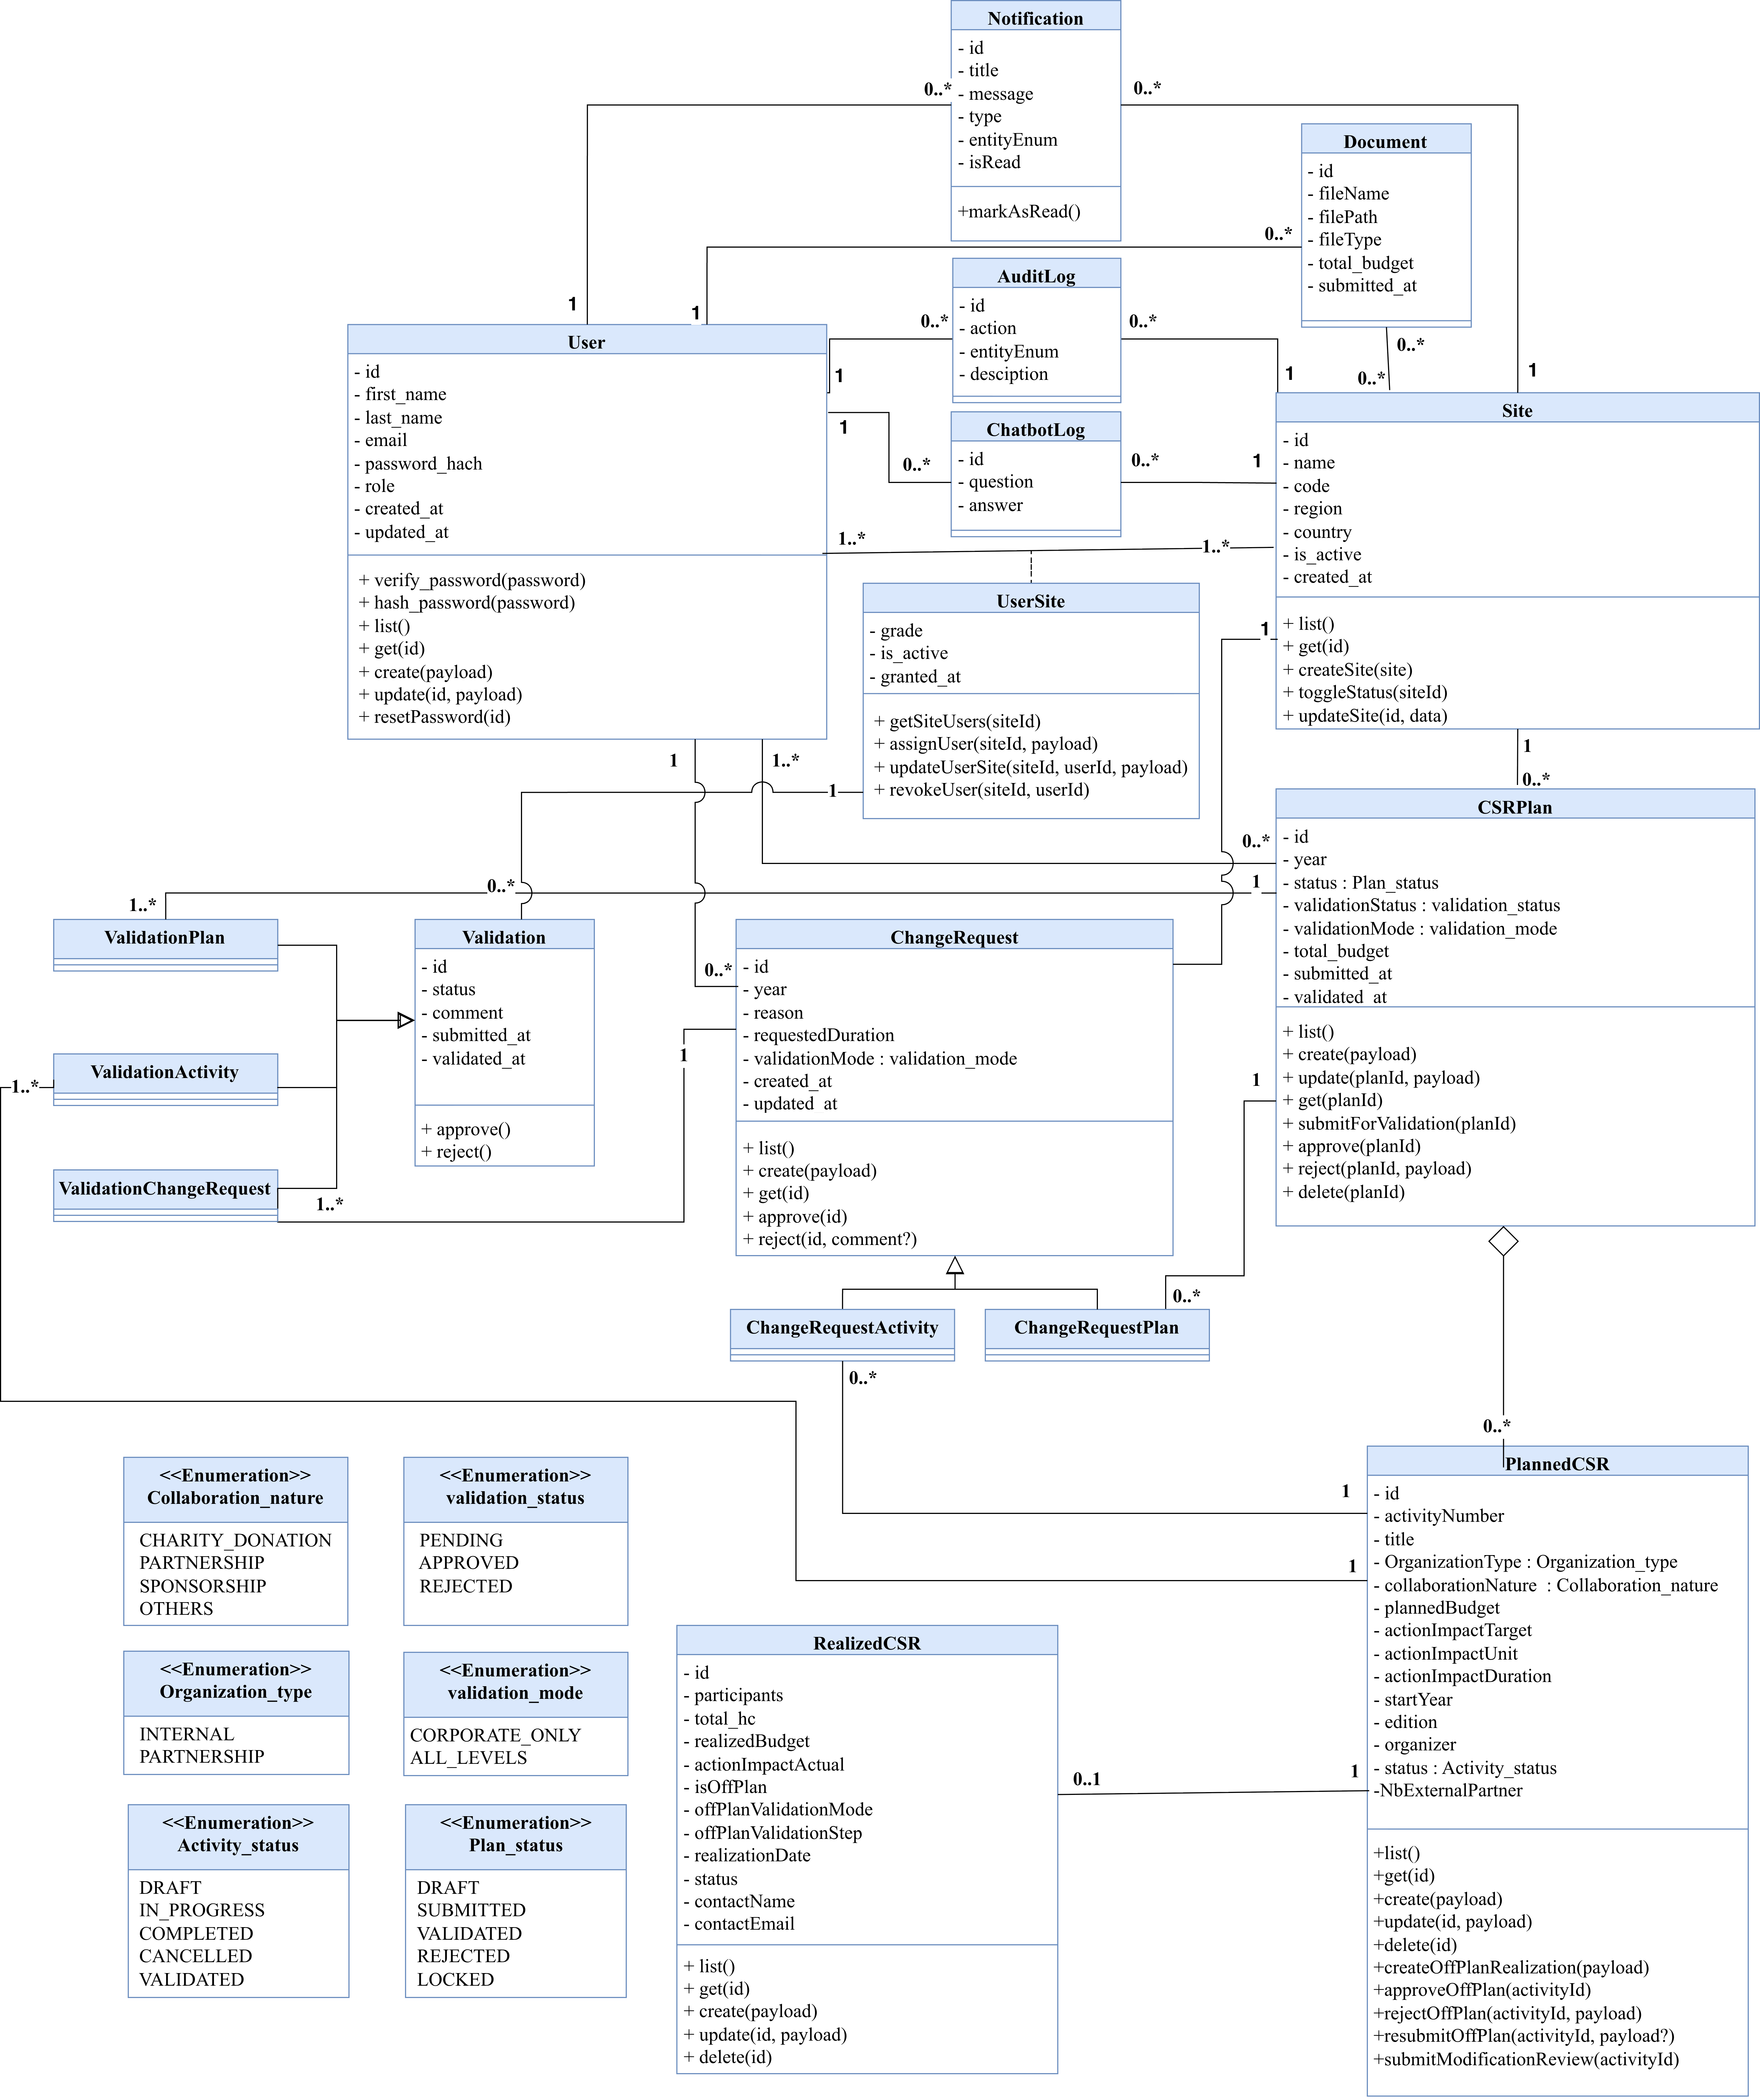
\includegraphics[width=0.92\linewidth]{figures/chapitre-05/diagramme-classe-workflow-transverse.png}
  \caption{Diagramme de classe — Gestion transverse des validations, notifications et traçabilité.}
  \label{fig:doc-ch5-2}
\end{figure}%

\subsection{Diagramme de séquence}

\subsubsection{Diagramme de séquence : «~Soumettre et traiter une demande de modification~»}

La figure~\ref{fig:doc-ch5-seq-cr} présente le scénario «~Soumettre et traiter une demande de modification~».

\IfFileExists{figures/chapitre-05/diagramme-sequence-demande-modification.png}{%
\begin{figure}[H]
  \centering
  \includegraphics[width=0.92\linewidth]{figures/chapitre-05/diagramme-sequence-demande-modification.png}
  \caption{Diagramme de séquence — demande de modification.}
  \label{fig:doc-ch5-seq-cr}
\end{figure}%
}{%
\begin{figure}[H]
  \centering
  \fbox{\parbox{0.92\linewidth}{\centering\vspace{3.2cm}\textit{(Figure à insérer : \texttt{figures/chapitre-05/diagramme-sequence-demande-modification.png})}\vspace{3.2cm}}}
  \caption{Diagramme de séquence — demande de modification.}
  \label{fig:doc-ch5-seq-cr}
\end{figure}%
}

\subsubsection{Diagramme de séquence : «~Propagation notification et tâches~»}

La figure~\ref{fig:doc-ch5-seq-notif} illustre la propagation \textbf{notification + tâche} après un événement métier.

\IfFileExists{figures/chapitre-05/diagramme-sequence-notification-tache.png}{%
\begin{figure}[H]
  \centering
  \includegraphics[width=0.92\linewidth]{figures/chapitre-05/diagramme-sequence-notification-tache.png}
  \caption{Diagramme de séquence — notification et rafraîchissement des tâches.}
  \label{fig:doc-ch5-seq-notif}
\end{figure}%
}{%
\begin{figure}[H]
  \centering
  \fbox{\parbox{0.92\linewidth}{\centering\vspace{3.2cm}\textit{(Figure à insérer : \texttt{figures/chapitre-05/diagramme-sequence-notification-tache.png})}\vspace{3.2cm}}}
  \caption{Diagramme de séquence — notification et rafraîchissement des tâches.}
  \label{fig:doc-ch5-seq-notif}
\end{figure}%
}

\section{Réalisation}

Dans cette partie, nous présentons les interfaces développées durant ce troisième sprint.
Les différentes captures illustrent les fonctionnalités mises en place, notamment le processus de validation des plans et des activités, la gestion des demandes de modification, ainsi que le suivi des notifications et des tâches.
Ces éléments permettent de visualiser concrètement le fonctionnement du workflow et de vérifier l'adéquation des fonctionnalités réalisées avec les exigences définies dans le backlog du sprint.

\subsection{Interface de validation des plans annuels}

La figure~\ref{fig:ch5-realisation-validation-plans} présente l'interface de validation des plans annuels.

\IfFileExists{figures/chapitre-05/realisation-interface-validation-plans-annuels.png}{%
\begin{figure}[H]
  \centering
  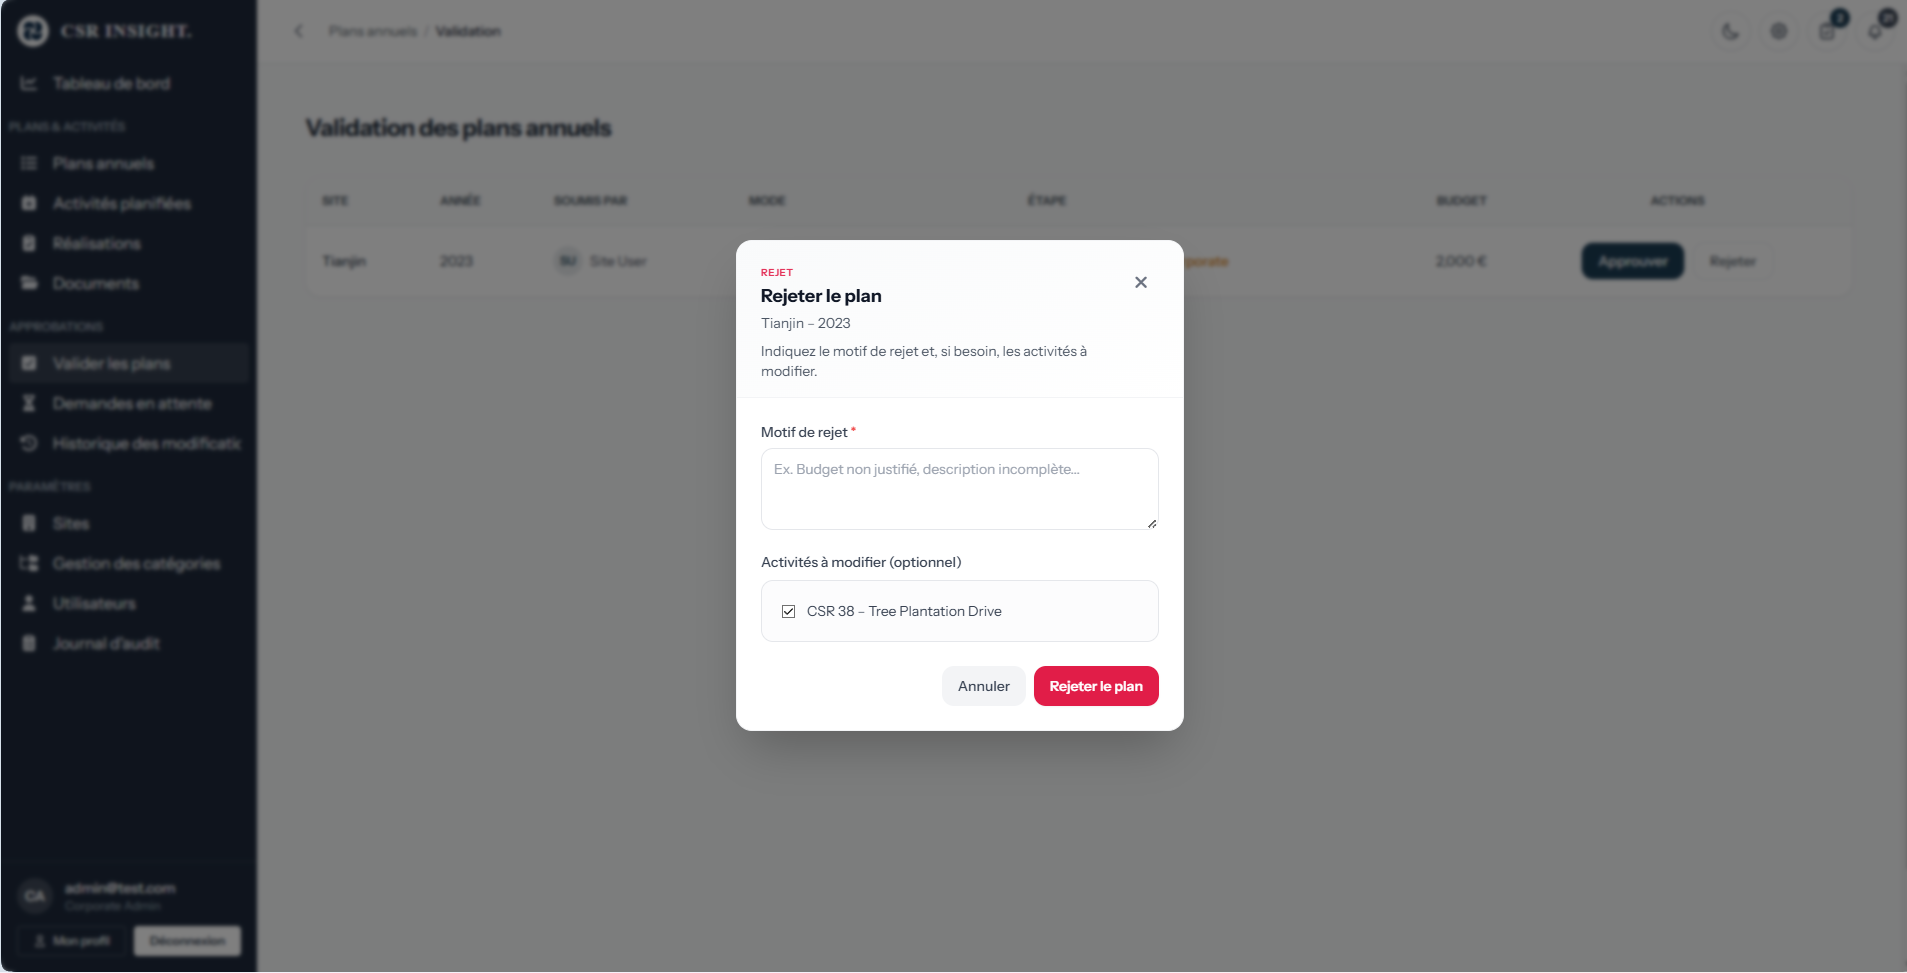
\includegraphics[width=0.92\linewidth]{figures/chapitre-05/realisation-interface-validation-plans-annuels.png}
  \caption{Interface de validation des plans annuels.}
  \label{fig:ch5-realisation-validation-plans}
\end{figure}%
}{%
\begin{figure}[H]
  \centering
  \fbox{\parbox{0.92\linewidth}{\centering\vspace{3.2cm}\textit{(Figure à insérer : \texttt{figures/chapitre-05/realisation-interface-validation-plans-annuels.png})}\vspace{3.2cm}}}
  \caption{Interface de validation des plans annuels.}
  \label{fig:ch5-realisation-validation-plans}
\end{figure}%
}

L'interface ci-dessus est dédiée à la validation des plans CSR, utilisée par l'utilisateur Corporate pour examiner les plans soumis.
Elle repose sur un tableau synthétique affichant les informations essentielles, notamment le site concerné, l'année, l'utilisateur ayant effectué la soumission, le mode de validation, l'état d'avancement ainsi que le budget associé.
Cette organisation permet d'identifier rapidement les plans en attente de décision.

Chaque ligne intègre des actions directes, telles que l'approbation ou le rejet, offrant une interaction rapide et efficace avec le système.
L'utilisateur peut ainsi traiter les demandes de validation de manière centralisée, tout en conservant une vision globale des éléments en cours.
Cette interface constitue un point clé du processus décisionnel, en facilitant le contrôle et la validation des données avant leur finalisation.

\subsection{Interface de rejet d'un plan}

La figure~\ref{fig:ch5-realisation-rejet-plan} présente l'interface de rejet d'un plan.

\IfFileExists{figures/chapitre-05/realisation-interface-rejet-plan.png}{%
\begin{figure}[H]
  \centering
  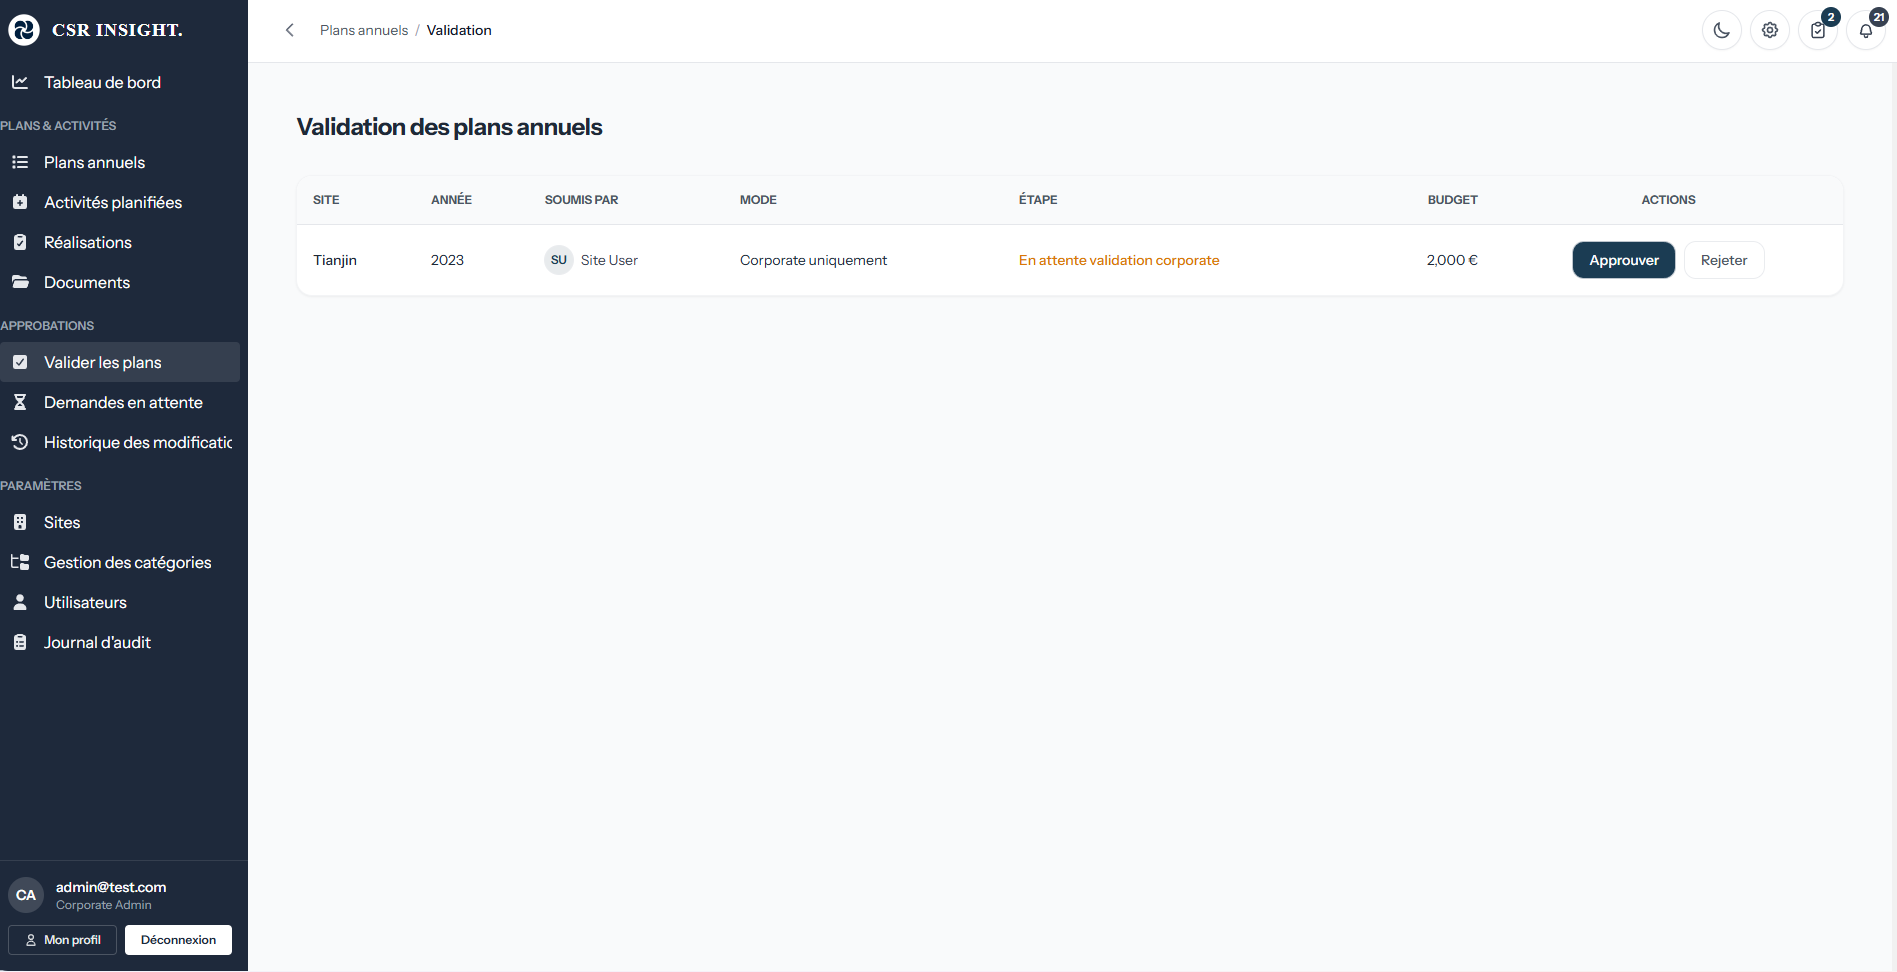
\includegraphics[width=0.92\linewidth]{figures/chapitre-05/realisation-interface-rejet-plan.png}
  \caption{Interface de rejet d'un plan.}
  \label{fig:ch5-realisation-rejet-plan}
\end{figure}%
}{%
\begin{figure}[H]
  \centering
  \fbox{\parbox{0.92\linewidth}{\centering\vspace{3.2cm}\textit{(Figure à insérer : \texttt{figures/chapitre-05/realisation-interface-rejet-plan.png})}\vspace{3.2cm}}}
  \caption{Interface de rejet d'un plan.}
  \label{fig:ch5-realisation-rejet-plan}
\end{figure}%
}

Cette interface illustre la fenêtre de rejet d'un plan, affichée lors de l'activation de l'action correspondante.
Elle permet à l'utilisateur Corporate de renseigner un motif de rejet, champ obligatoire garantissant la justification de la décision.
Elle offre également la possibilité de préciser, de manière optionnelle, les activités nécessitant des corrections.

L'objectif de cette interface est d'assurer un retour structuré et exploitable vers l'utilisateur à l'origine du plan, en encadrant le processus de correction.
Elle contribue également à renforcer la traçabilité des décisions prises, en conservant une justification claire associée à chaque rejet, tout en maintenant la cohérence du workflow global.

\subsection{Interface de demande de modification d'une activité}

La figure~\ref{fig:ch5-realisation-demande-modif-activite} présente l'interface de demande de modification d'une activité.

\IfFileExists{figures/chapitre-05/realisation-interface-demande-modification-activite.png}{%
\begin{figure}[H]
  \centering
  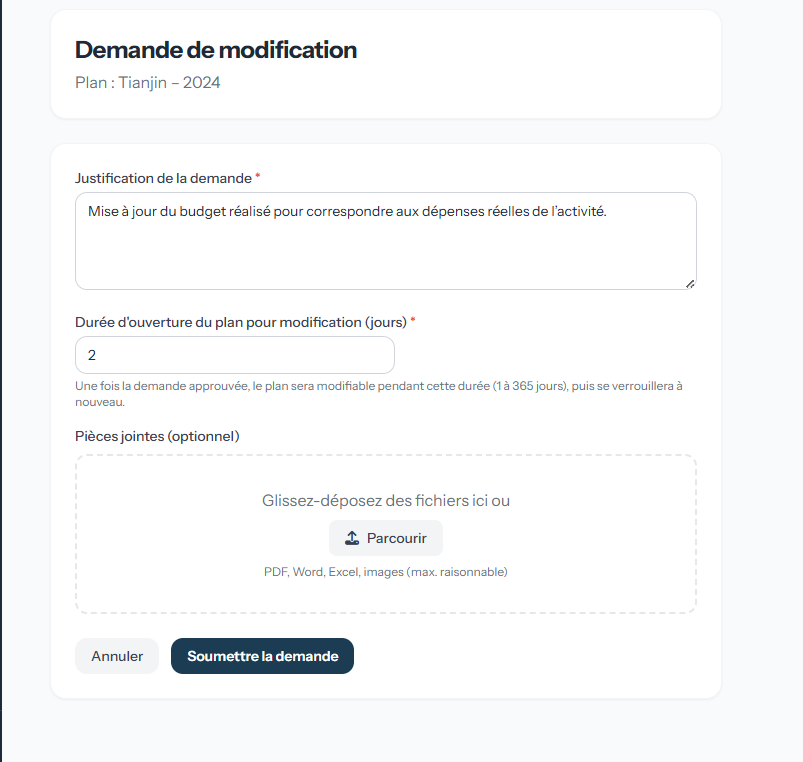
\includegraphics[width=0.92\linewidth]{figures/chapitre-05/realisation-interface-demande-modification-activite.png}
  \caption{Interface de demande de modification d'une activité.}
  \label{fig:ch5-realisation-demande-modif-activite}
\end{figure}%
}{%
\begin{figure}[H]
  \centering
  \fbox{\parbox{0.92\linewidth}{\centering\vspace{3.2cm}\textit{(Figure à insérer : \texttt{figures/chapitre-05/realisation-interface-demande-modification-activite.png})}\vspace{3.2cm}}}
  \caption{Interface de demande de modification d'une activité.}
  \label{fig:ch5-realisation-demande-modif-activite}
\end{figure}%
}

Cette interface présente la soumission d'une demande de modification d'une activité, permettant à l'utilisateur Site d'intervenir sur une activité déjà validée.
Elle se présente sous forme d'un formulaire structuré facilitant la saisie des informations nécessaires à l'analyse de la demande.

L'utilisateur doit renseigner une justification détaillée expliquant les raisons de la modification.
Il définit également une durée d'ouverture durant laquelle l'activité pourra être temporairement modifiée après approbation.
Une section spécifique permet d'ajouter des pièces jointes afin d'appuyer la demande avec des éléments justificatifs pertinents.

L'interface intègre des contrôles de validation pour garantir la complétude des informations avant la soumission.
Une fois envoyée, la demande est enregistrée et transmise à l'utilisateur Corporate pour traitement.
Elle s'inscrit ainsi dans un processus de contrôle post-validation, permettant de corriger les données tout en assurant la traçabilité et la cohérence du système.

\subsection{Interface du journal d'audit}

La figure~\ref{fig:ch5-realisation-journal-audit} présente l'interface du journal d'audit.

\IfFileExists{figures/chapitre-05/realisation-interface-journal-audit.png}{%
\begin{figure}[H]
  \centering
  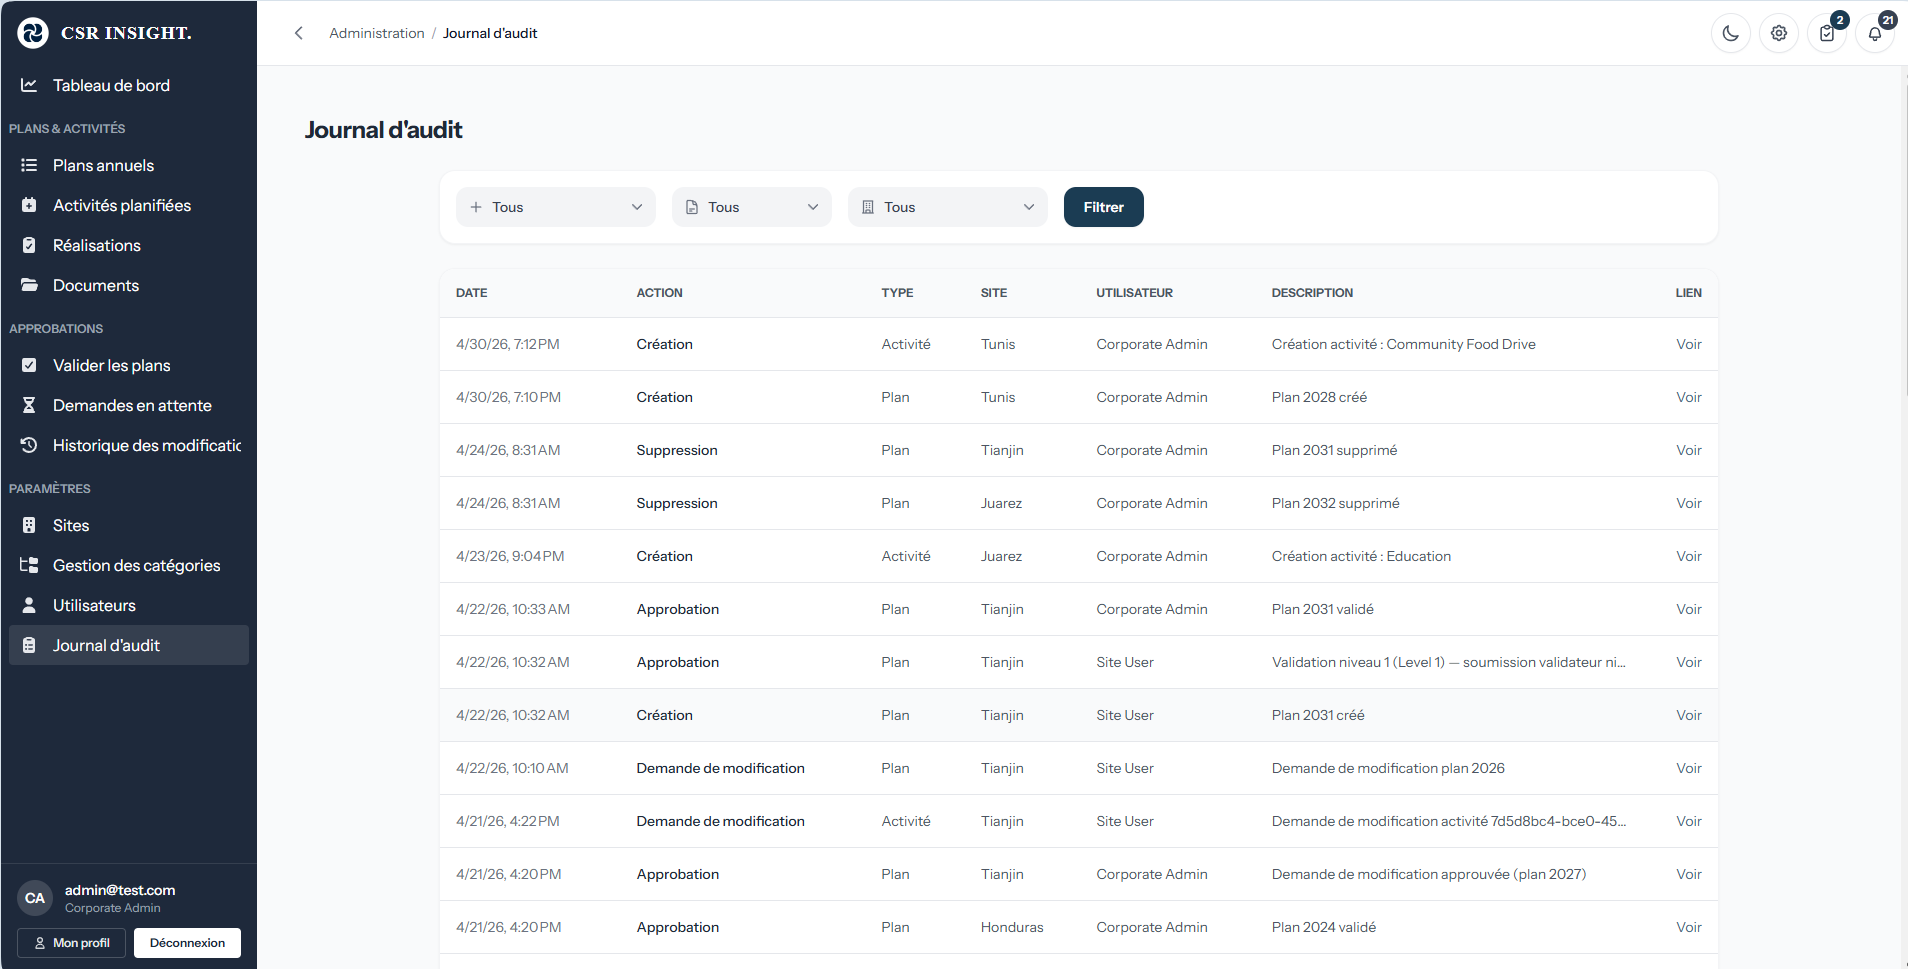
\includegraphics[width=0.92\linewidth]{figures/chapitre-05/realisation-interface-journal-audit.png}
  \caption{Interface du journal d'audit.}
  \label{fig:ch5-realisation-journal-audit}
\end{figure}%
}{%
\begin{figure}[H]
  \centering
  \fbox{\parbox{0.92\linewidth}{\centering\vspace{3.2cm}\textit{(Figure à insérer : \texttt{figures/chapitre-05/realisation-interface-journal-audit.png})}\vspace{3.2cm}}}
  \caption{Interface du journal d'audit.}
  \label{fig:ch5-realisation-journal-audit}
\end{figure}%
}

L'interface du journal d'audit est conçue pour assurer le suivi et la traçabilité de l'ensemble des actions effectuées sur la plateforme.
Ce module est accessible uniquement aux utilisateurs Corporate, afin de garantir un contrôle centralisé et sécurisé des opérations réalisées sur le système.

Elle offre une vue structurée sous forme de tableau chronologique regroupant les événements liés aux différentes entités, notamment les plans et les activités.
Chaque enregistrement détaille des informations clés telles que la date et l'heure de l'action, son type (création, validation, suppression, demande de modification, etc.), l'entité concernée, le site associé ainsi que l'utilisateur à l'origine de l'opération.
Une description explicite permet de comprendre rapidement le contexte de chaque action, avec la possibilité d'accéder directement à l'élément concerné.

Des options de filtrage sont également disponibles pour affiner l'affichage selon plusieurs critères, facilitant ainsi la recherche et l'analyse des opérations.
Cette interface constitue un élément essentiel du système, en assurant la transparence, la traçabilité et le suivi rigoureux de toutes les actions dans le cadre du workflow global.

\section{Tests et validation}

Les tests occupent une place centrale dans la méthodologie agile, car ils garantissent la qualité ainsi que la fiabilité des fonctionnalités développées. Avant le lancement d'un nouveau sprint, il est indispensable de valider les incréments prioritaires afin de vérifier leur bon fonctionnement et leur conformité aux besoins des parties prenantes.

\subsection{Test}

Dans cette partie, nous présentons une validation fonctionnelle consolidée des fonctionnalités du sprint~3 : validation et rejet des plans CSR, demandes de modification (plan), notifications, tâches et consultation du journal d'audit.
Le tableau~\ref{tab:ch5-scenarios-tests} synthétise les cas de test correspondants.

% Scénarios de test consolidés — chapitre 5 (workflow transverse)
\small
\PFETableSetup
\setlength{\LTpre}{0pt}
\setlength{\LTpost}{0pt}
\setlength{\LTleft}{\fill}
\setlength{\LTright}{\fill}
\setlength{\tabcolsep}{3.5pt}
\renewcommand{\arraystretch}{1.25}

\begin{longtable}{|>{\centering\arraybackslash}m{2.8cm}|
>{\raggedright\arraybackslash}p{2.5cm}|
>{\raggedright\arraybackslash}p{3.8cm}|
>{\raggedright\arraybackslash}p{4.3cm}|
>{\centering\arraybackslash}p{1.1cm}|}
\caption{Synthèse des cas de test du sprint 3}\label{tab:ch5-scenarios-tests}\\
\hline
\tableHeaderStyle
\multicolumn{1}{|c|}{\tableHeaderCell{Nom du cas d'utilisation}} &
\multicolumn{1}{c|}{\tableHeaderCell{Cas de test}} &
\multicolumn{1}{c|}{\tableHeaderCell{Description du cas}} &
\multicolumn{1}{c|}{\tableHeaderCell{Résultat attendu}} &
\multicolumn{1}{c|}{\tableHeaderCell{Résultat réel}} \\
\hline
\endfirsthead
\hline
\multicolumn{5}{|c|}{\tablename\ \thetable{} --- \textit{(suite)}} \\
\hline
\tableHeaderStyle
\multicolumn{1}{|c|}{\tableHeaderCell{Nom du cas d'utilisation}} &
\multicolumn{1}{c|}{\tableHeaderCell{Cas de test}} &
\multicolumn{1}{c|}{\tableHeaderCell{Description du cas}} &
\multicolumn{1}{c|}{\tableHeaderCell{Résultat attendu}} &
\multicolumn{1}{c|}{\tableHeaderCell{Résultat réel}} \\
\hline
\endhead
\hline
\multicolumn{5}{|r|}{\textit{Suite page suivante\ldots}} \\
\hline
\endfoot
\hline
\endlastfoot

\needspace{18\baselineskip}
\multirow{3}{=}{\centering Valider un plan CSR} &
Validation corporate (mode direct) &
Un utilisateur Corporate valide un plan soumis lorsque le mode le permet sans étape site préalable. &
Le plan passe au statut validé et n'est plus modifiable. &
Vrai \\
\cline{2-5}
 &
Validation en deux étapes &
Le Corporate tente de valider avant la validation du site lorsque le mode l'exige. &
Le système refuse et indique que la validation du site est requise en premier. &
Vrai \\
\cline{2-5}
 &
Consultation liste des plans soumis &
Ouverture de l'interface listant les plans en attente de décision. &
Les informations essentielles (site, année, statut, budget) sont affichées. &
Vrai \\
\hline

\needspace{12\baselineskip}
\multirow{2}{=}{\centering Rejeter un plan CSR} &
Motif obligatoire manquant &
Tentative de rejet sans saisir le motif de rejet. &
La soumission est refusée et le champ motif est signalé comme obligatoire. &
Vrai \\
\cline{2-5}
 &
Rejet avec motif valide &
Saisie d'un motif de rejet et confirmation du rejet. &
Le plan est rejeté, le statut est mis à jour et le motif est conservé. &
Vrai \\
\hline

\needspace{18\baselineskip}
\multirow{3}{=}{\centering Soumettre une demande\\de modification pour un plan} &
Données incomplètes &
Soumission d'une demande sans justification ou sans durée d'ouverture requise. &
Message d'erreur listant les champs à compléter. &
Vrai \\
\cline{2-5}
 &
Pièce jointe non conforme &
Ajout d'un fichier de type ou taille non autorisé. &
Le fichier est refusé avec un message explicite. &
Vrai \\
\cline{2-5}
 &
Soumission valide &
Demande complète sur un plan verrouillé avec justification et durée. &
La demande est enregistrée avec le statut « en attente » et associée au plan. &
Vrai \\
\hline

\needspace{12\baselineskip}
\multirow{2}{=}{\centering Traiter une demande\\de modification} &
Approbation corporate &
Examen puis approbation d'une demande en attente. &
Le statut de la demande est mis à jour et le site est notifié. &
Vrai \\
\cline{2-5}
 &
Rejet avec justification &
Rejet d'une demande avec commentaire obligatoire. &
Le statut est mis à jour et le motif est conservé pour le site. &
Vrai \\
\hline

\needspace{12\baselineskip}
\multirow{2}{=}{\centering Recevoir des\\notifications} &
Notification après validation &
Un événement de validation génère une notification pour les acteurs concernés. &
La notification apparaît dans le centre de notifications. &
Vrai \\
\cline{2-5}
 &
Marquer comme lue &
L'utilisateur ouvre ou marque une notification comme lue. &
L'état de lecture est mis à jour et le compteur reflète le changement. &
Vrai \\
\hline

\needspace{12\baselineskip}
\multirow{2}{=}{\centering Gérer les tâches} &
Tâche créée après un événement &
Soumission ou validation déclenchant la création d'une tâche assignée. &
La tâche apparaît dans la liste des tâches de l'utilisateur concerné. &
Vrai \\
\cline{2-5}
 &
Ouverture d'une tâche &
Clic sur une tâche pour accéder au contexte (plan ou demande). &
La navigation mène à l'écran attendu. &
Vrai \\
\hline

\needspace{12\baselineskip}
\multirow{2}{=}{\centering Consulter le\\journal d'audit} &
Affichage chronologique &
Consultation de la liste des événements par un profil Corporate autorisé. &
Les actions sont listées avec date, type, entité et auteur. &
Vrai \\
\cline{2-5}
 &
Filtrage par critères &
Application de filtres (site, type d'action, période). &
La liste se restreint aux enregistrements correspondants. &
Vrai \\
\hline

\end{longtable}
\normalsize


\newpage

Les flux liés aux demandes de modification, aux notifications et aux tâches ont également été vérifiés avec \emph{Postman}, en contrôlant les réponses après enchaînement des actions corporate.
Les figures~\ref{fig:ch5-postman-cr},~\ref{fig:ch5-postman-notif} et~\ref{fig:ch5-postman-tasks} illustrent des exemples de ces vérifications.

\IfFileExists{figures/chapitre-05/postman-change-requests.png}{%
\begin{figure}[H]
  \centering
  \includegraphics[width=0.92\linewidth]{figures/chapitre-05/postman-change-requests.png}
  \caption{Tests Postman : demandes de modification.}
  \label{fig:ch5-postman-cr}
\end{figure}%
}{%
\begin{figure}[H]
  \centering
  \fbox{\parbox{0.92\linewidth}{\centering\vspace{3.2cm}\textit{(Figure à insérer : \texttt{figures/chapitre-05/postman-change-requests.png})}\vspace{3.2cm}}}
  \caption{Tests Postman : demandes de modification.}
  \label{fig:ch5-postman-cr}
\end{figure}%
}

\IfFileExists{figures/chapitre-05/postman-notifications.png}{%
\begin{figure}[H]
  \centering
  \includegraphics[width=0.92\linewidth]{figures/chapitre-05/postman-notifications.png}
  \caption{Tests Postman : notifications.}
  \label{fig:ch5-postman-notif}
\end{figure}%
}{%
\begin{figure}[H]
  \centering
  \fbox{\parbox{0.92\linewidth}{\centering\vspace{3.2cm}\textit{(Figure à insérer : \texttt{figures/chapitre-05/postman-notifications.png})}\vspace{3.2cm}}}
  \caption{Tests Postman : notifications.}
  \label{fig:ch5-postman-notif}
\end{figure}%
}

\IfFileExists{figures/chapitre-05/postman-tasks.png}{%
\begin{figure}[H]
  \centering
  \includegraphics[width=0.92\linewidth]{figures/chapitre-05/postman-tasks.png}
  \caption{Tests Postman : tâches.}
  \label{fig:ch5-postman-tasks}
\end{figure}%
}{%
\begin{figure}[H]
  \centering
  \fbox{\parbox{0.92\linewidth}{\centering\vspace{3.2cm}\textit{(Figure à insérer : \texttt{figures/chapitre-05/postman-tasks.png})}\vspace{3.2cm}}}
  \caption{Tests Postman : tâches.}
  \label{fig:ch5-postman-tasks}
\end{figure}%
}

\subsection{Validation}

Une revue de fin de sprint avec le \emph{Scrum Master} et le \emph{Product Owner} a permis de valider les parcours du sprint 3 : Gestion transverse des validations, notifications et traçabilité (validation et rejet de plans, demandes de modification, notifications, tâches et journal d'audit). Les correctifs portent notamment sur les messages utilisateur, la cohérence des statuts entre demandes et entités concernées, ainsi que sur le rafraîchissement des listes après action corporate.

\section{Conclusion}

Ce sprint renforce la gouvernance des données CSR en introduisant un mécanisme de gestion globale:
contrôle des validations, traitement des demandes de modification, notifications, tâches et audit.

Le chapitre suivant présente le sprint \emph{BI \& KPI} (tableaux de bord, intégration Power BI et indicateurs de pilotage).



% ------\input{chapters/chapitre-06-sprint4-bi-kpi}

% ----- Conclusion générale -----
\cleardoublepage
% Conclusion (hors numérotation de chapitre)
\PFEDedicatedChapterPage{Conclusion générale}
\PFEChapterSilentHeadtrue
\chapter*{Conclusion générale}
\PFEChapterSilentHeadfalse
\addcontentsline{toc}{chapter}{Conclusion générale}
Synthèse finale.


% ----- Webographie / Références -----
\cleardoublepage
\chapter*{Webographie}
\addcontentsline{toc}{chapter}{Webographie}

\begin{thebibliography}{99}
\bibitem{elloumi-website}
Groupe Elloumi, \textit{Site officiel du Groupe Elloumi}. Consulté le 03/02/2026. \url{https://www.elloumi.com/}
    
\bibitem{coficab-website}
COFICAB, \textit{Site officiel de COFICAB}. Consulté le 03/02/2026. \url{https://www.coficab.com/}

\bibitem{global-footprint-coficab}
COFICAB, \textit{Global Footprint - COFICAB Group}. Consulté le 03/02/2026. \url{https://www.coficab.com/global-footprint/}
\bibitem{odoo-docs}
Odoo, \textit{Odoo Documentation}. Consulté le 14/04/2026. \url{https://www.odoo.com/documentation/17.0/}

\bibitem{powerbi-docs}
Microsoft, \textit{Power BI Documentation}. Consulté le 14/04/2026. \url{https://learn.microsoft.com/power-bi/}

\bibitem{mes-docs}
MES, \textit{MES Documentation}. Consulté le 14/04/2026. \url{https://www.mes.com/}

\bibitem{trello-docs}
Trello, \textit{Trello Documentation}. Consulté le 14/04/2026. \url{https://trello.com/documentation/}

\bibitem{monday-docs}
Monday.com, \textit{Monday.com Help Center}. Consulté le 01/05/2026. \url{https://support.monday.com/hc/en-us}

\bibitem{Generous-Connect}
Generous Connect, \textit{Generous Connect Documentation}. Consulté le 14/04/2026. \url{https://www.generousconnect.com/documentation/}

\bibitem{Optimy}
Optimy, \textit{Optimy Documentation}. Consulté le 14/04/2026. \url{https://www.optimy.com/documentation/}

\bibitem{pm-partners-scrum-overview}
PM Partners, \textit{The Agile Journey: A Scrum Overview}. Consulté le 14/04/2026. \url{https://www.pm-partners.com.au/insights/the-agile-journey-a-scrum-overview/}

\bibitem{sketchbubble-rup}
SketchBubble, \textit{Rational Unified Process (RUP) (presentation)}. Consulté le 14/04/2026. \url{https://www.sketchbubble.com/en/presentation-rational-unified-process.html}

\bibitem{headmind-bi-intro}
HeadMind Partners, \textit{Business Intelligence: Introduction}. Consulté le 14/04/2026. \url{https://www.headmind.com/en/business-intelligence-introduction/}

\bibitem{pacheco-stacey-matrix}
J. F. Pacheco, \textit{Navigating the Maze: Mastering the Stacey Matrix for Project Success}. Consulté le 14/04/2026. \url{https://juanfernandopacheco.medium.com/navigating-the-maze-mastering-the-stacey-matrix-for-project-success-313d27764987}

\bibitem{angular-docs}
Google / Angular Team, \textit{Angular — documentation officielle}. Consulté le 14/04/2026. \url{https://angular.dev/}

\bibitem{flask-docs}
Pallets Projects, \textit{Flask — documentation}. Consulté le 14/04/2026. \url{https://flask.palletsprojects.com/en/stable/}

\bibitem{mysql-docs}
Oracle / MySQL, \textit{MySQL 8.4 Reference Manual}. Consulté le 14/04/2026. \url{https://dev.mysql.com/doc/refman/8.4/en/}

\bibitem{sqlalchemy-docs}
SQLAlchemy, \textit{SQLAlchemy Documentation}. Consulté le 14/04/2026. \url{https://docs.sqlalchemy.org/en/20/}

\bibitem{primeng-docs}
PrimeTek, \textit{PrimeNG — documentation}. Consulté le 14/04/2026. \url{https://primeng.org/}

\bibitem{socketio-docs}
Socket.IO, \textit{Socket.IO Documentation}. Consulté le 14/04/2026. \url{https://socket.io/docs/v4/}

\bibitem{postman-docs}
Postman, \textit{Postman Learning Center}. Consulté le 29/04/2026. \url{https://learning.postman.com/}

\bibitem{python-docs}
Python Software Foundation, \textit{The Python Language Reference}. Consulté le 14/04/2026. \url{https://docs.python.org/3/reference/index.html}

\bibitem{typescript-docs}
Microsoft / TypeScript, \textit{TypeScript Documentation}. Consulté le 14/04/2026. \url{https://www.typescriptlang.org/docs/}

\bibitem{tailwind-docs}
Tailwind Labs, \textit{Tailwind CSS — documentation}. Consulté le 14/04/2026. \url{https://tailwindcss.com/docs}

\bibitem{heidisql-docs}
Ansgar Becker, \textit{HeidiSQL — aide et documentation}. Consulté le 14/04/2026. \url{https://www.heidisql.com/help.php}

\bibitem{vscode-docs}
Microsoft, \textit{Visual Studio Code — documentation}. Consulté le 14/04/2026. \url{https://code.visualstudio.com/docs}

\bibitem{diagrams-net-docs}
JGraph Ltd, \textit{diagrams.net (draw.io) — documentation}. Consulté le 14/04/2026. \url{https://www.diagrams.net/doc}

\bibitem{git-docs}
Software Freedom Conservancy, \textit{Git — documentation}. Consulté le 14/04/2026. \url{https://git-scm.com/doc}

\bibitem{github-docs}
GitHub, \textit{GitHub Docs}. Consulté le 14/04/2026. \url{https://docs.github.com/}

\bibitem{xampp-docs}
Apache Friends, \textit{XAMPP — documentation}. Consulté le 14/04/2026. \url{https://www.apachefriends.org/}

\bibitem{latex-docs}
The \LaTeX\ Project, \textit{\LaTeX\ documentation}. Consulté le 14/04/2026. \url{https://www.latex-project.org/help/documentation/}

\bibitem{visualstudio-docs}
Microsoft, \textit{Visual Studio — documentation}. Consulté le 14/04/2026. \url{https://learn.microsoft.com/visualstudio/}

\bibitem{sqlserver-docs}
Microsoft, \textit{SQL Server — documentation}. Consulté le 14/04/2026. \url{https://learn.microsoft.com/sql/sql-server/}

\bibitem{ssms-docs}
Microsoft, \textit{SQL Server Management Studio (SSMS) — documentation}. Consulté le 15/04/2026. \url{https://learn.microsoft.com/sql/ssms/sql-server-management-studio-ssms}

\bibitem{ssis-docs}
Microsoft, \textit{SQL Server Integration Services — documentation}. Consulté le 15/04/2026. \url{https://learn.microsoft.com/sql/integration-services/sql-server-integration-services}

\bibitem{orm-wikipedia}
Wikipédia, \textit{Mapping objet-relationnel}. Consulté le 15/04/2026. \url{https://fr.wikipedia.org/wiki/Mapping_objet-relationnel}

\end{thebibliography}



% ----- Annexes -----
\appendix
% Annexe A (après \appendix dans main.tex)
\PFEChapterOpening{Première annexe}
\label{chap:annexe-premiere}

\section{Matrice de Stacey}

\begin{figure}[H]
  \centering
  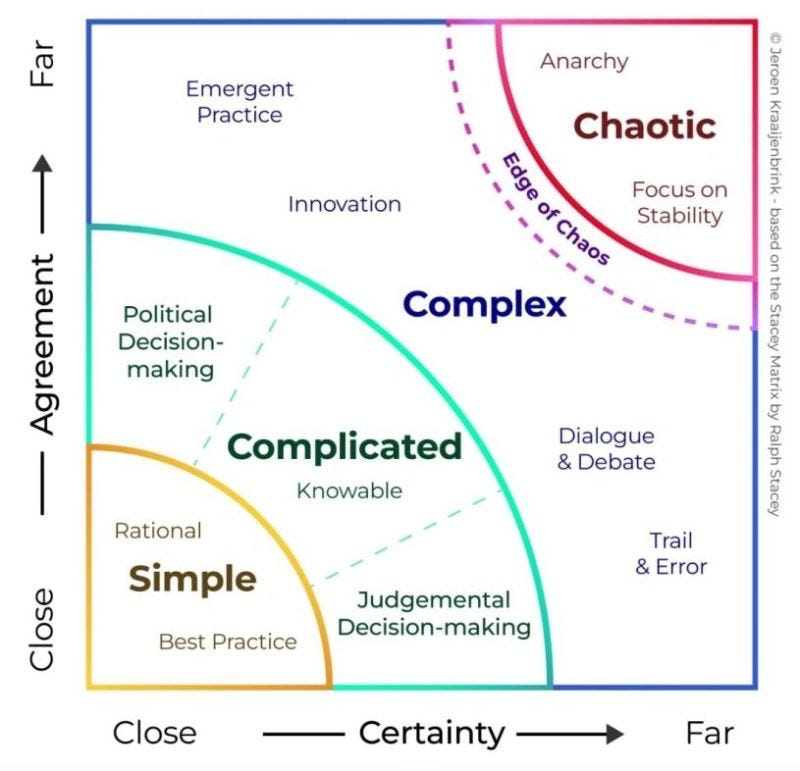
\includegraphics[width=0.75\linewidth]{figures/chapitre-01/matrice-stacey.png}
  \caption{Matrice de Stacey.}\cite{pacheco-stacey-matrix}
  \label{fig:annexe-matrice-stacey}
\end{figure}

% Annexe B — Dictionnaire de données (diagramme de classes général)
\PFEChapterOpening{Dictionnaire de données du diagramme de classes général}
\label{chap:annexe-dictionnaire-donnees}

% Dictionnaire de données : même style visuel que tables/chapitre-01-tab-synthese.tex
% (tabularx, \PFETableSetup, bandeau d'en-tête, lignes alternées, sans filets verticaux).
% Table un peu plus large que \textwidth et centrée sur la page (comme chapitre-02-product-backlog).
\begingroup
\small
\setlength{\PFEdictTabW}{\dimexpr\textwidth+26mm\relax}
\setlength{\LTcapwidth}{\PFEdictTabW}
\setlength{\LTleft}{\dimexpr(\textwidth-\PFEdictTabW)/2\relax}
\setlength{\LTright}{\dimexpr(\textwidth-\PFEdictTabW)/2\relax}
\setlength{\LTpre}{4pt}
\setlength{\LTpost}{6pt}
\PFETableSetup
\PFETableRowColors
\PFETableArrayStretch
\PFETableTabularXBegin
\begin{xltabular}{\PFEdictTabW}{@{}%
  >{\centering\arraybackslash\hsize=0.5\hsize}X%
  >{\raggedright\arraybackslash\hsize=1.0\hsize}X%
  >{\raggedright\arraybackslash\hsize=1.65\hsize}X%
  >{\raggedright\arraybackslash\hsize=0.85\hsize}X%
@{}}
  \caption{Dictionnaire de données du diagramme de classes général.}
  \label{tab:dictionnaire-donnees-classe} \\
  \tableHeaderStyle
  \tableHeaderCell{N\textsuperscript{o}} &
  \tableHeaderCell{Attribut} &
  \tableHeaderCell{Libellé} &
  \tableHeaderCell{Type} \\
  \endfirsthead
  \multicolumn{4}{c}{\small\itshape Suite du tableau~\ref{tab:dictionnaire-donnees-classe}.} \\
  \tableHeaderStyle
  \tableHeaderCell{N\textsuperscript{o}} &
  \tableHeaderCell{Attribut} &
  \tableHeaderCell{Libellé} &
  \tableHeaderCell{Type} \\
  \endhead
  \endfoot
  \endlastfoot
  \multicolumn{4}{@{}l@{}}{\cellcolor{tableHeader}\textcolor{white}{\textbf{Classe User} (\texttt{users})}} \\
  1 & \texttt{id} & Identifiant unique de l'utilisateur & \texttt{CHAR(36)} \\
  2 & \texttt{first\_name} & Prénom & \texttt{VARCHAR(255)} \\
  3 & \texttt{last\_name} & Nom & \texttt{VARCHAR(255)} \\
  4 & \texttt{email} & Adresse email (identifiant de connexion) & \texttt{VARCHAR(255)} \\
  5 & \texttt{password\_hach} & Mot de passe hashé (schéma ; colonne ORM \texttt{password\_hash}) & \texttt{VARCHAR(255)} \\
  6 & \texttt{role} & Rôle (\texttt{SITE\_USER} / \texttt{CORPORATE\_USER}) & \texttt{VARCHAR(50)} \\
  7 & \texttt{is\_active} & Compte actif ou désactivé & \texttt{BOOLEAN} \\
  8 & \texttt{is\_corporate\_global} & Accès corporate global (tous les sites) & \texttt{BOOLEAN} \\
  \multicolumn{4}{@{}l@{}}{\cellcolor{tableHeader}\textcolor{white}{\textbf{Classe Site} (\texttt{sites})}} \\
  9 & \texttt{id} & Identifiant unique du site & \texttt{CHAR(36)} \\
  10 & \texttt{name} & Nom du site & \texttt{VARCHAR(255)} \\
  11 & \texttt{code} & Code du site (ex.\ COFXX) & \texttt{VARCHAR(50)} \\
  12 & \texttt{region} & Région (ex.\ EE, America) & \texttt{VARCHAR(255)} \\
  13 & \texttt{country} & Pays & \texttt{VARCHAR(255)} \\
  14 & \texttt{is\_active} & Site actif ou non & \texttt{BOOLEAN} \\
  \multicolumn{4}{@{}l@{}}{\cellcolor{tableHeader}\textcolor{white}{\textbf{Classe UserSite} (\texttt{user\_sites})}} \\
  15 & \texttt{id} & Identifiant de l'association utilisateur--site & \texttt{CHAR(36)} \\
  16 & \texttt{grade} & Niveau d'accès sur le site & \texttt{VARCHAR(20)} \\
  17 & \texttt{is\_active} & Accès actif ou non & \texttt{BOOLEAN} \\
  \multicolumn{4}{@{}l@{}}{\cellcolor{tableHeader}\textcolor{white}{\textbf{Classe UserSession} (\texttt{user\_sessions})}} \\
  18 & \texttt{id} & Identifiant de la session & \texttt{CHAR(36)} \\
  19 & \texttt{refresh\_token} & Jeton de rafraîchissement & \texttt{VARCHAR(512)} \\
  20 & \texttt{is\_expires} & Date d'expiration (équivalent ORM \texttt{expires\_at}) & \texttt{DATETIME} \\
  \multicolumn{4}{@{}l@{}}{\cellcolor{tableHeader}\textcolor{white}{\textbf{Classe CSRPlan} (\texttt{csr\_plans})}} \\
  21 & \texttt{id} & Identifiant du plan & \texttt{CHAR(36)} \\
  22 & \texttt{year} & Année du plan & \texttt{INTEGER} \\
  23 & \texttt{status} & Statut du plan (brouillon, soumis, validé, etc.) & \texttt{VARCHAR(30)} \\
  24 & \texttt{validation\_mode} & Mode de validation (\texttt{101} / \texttt{111}) & \texttt{VARCHAR(10)} \\
  25 & \texttt{total\_budget} & Budget total du plan (€) & \texttt{DECIMAL(15,2)} \\
  26 & \texttt{submitted\_at} & Date de soumission & \texttt{DATETIME} \\
  27 & \texttt{validated\_at} & Date de validation finale & \texttt{DATETIME} \\
  \multicolumn{4}{@{}l@{}}{\cellcolor{tableHeader}\textcolor{white}{\textbf{Classe PlannedCSR} (\texttt{planned\_activity})}} \\
  28 & \texttt{id} & Identifiant de l'activité & \texttt{CHAR(36)} \\
  29 & \texttt{activityNumber} & Numéro d'activité (ORM \texttt{activity\_number}) & \texttt{VARCHAR(50)} \\
  30 & \texttt{title} & Titre / intitulé & \texttt{VARCHAR(255)} \\
  31 & \texttt{collaborationNature} & Nature de la collaboration (ORM \texttt{collaboration\_nature}) & \texttt{VARCHAR(30)} \\
  32 & \texttt{periodicity} & Périodicité & \texttt{VARCHAR(100)} \\
  33 & \texttt{plannedBudget} & Budget prévu (€) (ORM \texttt{planned\_budget}) & \texttt{DECIMAL(15,2)} \\
  34 & \texttt{actionImpactTarget} & Objectif d'impact (nombre) (ORM \texttt{action\_impact\_target}) & \texttt{DECIMAL(15,2)} \\
  35 & \texttt{actionImpactUnit} & Unité d'impact cible (ORM \texttt{action\_impact\_unit}) & \texttt{VARCHAR(100)} \\
  36 & \texttt{actionImpactDuration} & Durée de l'impact (ORM \texttt{action\_impact\_duration}) & \texttt{VARCHAR(100)} \\
  37 & \texttt{startYear} & Année de démarrage (ORM \texttt{start\_year}) & \texttt{INTEGER} \\
  38 & \texttt{edition} & Numéro d'édition & \texttt{INTEGER} \\
  39 & \texttt{organizer} & Organisateur (ex.\ HR) & \texttt{VARCHAR(255)} \\
  40 & \texttt{status} & Statut de l'activité & \texttt{VARCHAR(20)} \\
  41 & \texttt{NbExternalPartner} & Nombre de partenaires externes (ORM \texttt{number\_external\_partners}) & \texttt{INTEGER} \\
  \multicolumn{4}{@{}l@{}}{\cellcolor{tableHeader}\textcolor{white}{\textbf{Classe RealizedCSR} (\texttt{realized\_csr})}} \\
  42 & \texttt{id} & Identifiant de la réalisation & \texttt{CHAR(36)} \\
  43 & \texttt{participants} & Nombre de participants internes & \texttt{INTEGER} \\
  44 & \texttt{total\_hc} & Effectif total du site & \texttt{INTEGER} \\
  45 & \texttt{realizedBudget} & Budget réel dépensé (€) (ORM \texttt{realized\_budget}) & \texttt{DECIMAL(15,2)} \\
  46 & \texttt{actionImpactActual} & Impact réalisé (nombre) (ORM \texttt{action\_impact\_actual}) & \texttt{DECIMAL(15,2)} \\
  47 & \texttt{actionImpactUnit} & Unité d'impact réalisée (ORM \texttt{action\_impact\_unit}) & \texttt{VARCHAR(100)} \\
  48 & \texttt{isOffPlan} & Activité hors plan (ORM \texttt{is\_off\_plan}) & \texttt{BOOLEAN} \\
  49 & \texttt{offPlanValidationMode} & Mode validation hors plan (ORM \texttt{off\_plan\_validation\_mode}) & \texttt{VARCHAR(10)} \\
  50 & \texttt{offPlanValidationStep} & Étape de validation (ORM \texttt{off\_plan\_validation\_step}) & \texttt{INTEGER} \\
  51 & \texttt{realizationDate} & Date de réalisation (ORM \texttt{realization\_date}) & \texttt{DATE} \\
  52 & \texttt{status} & Statut de la réalisation & \texttt{VARCHAR(20)} \\
  53 & \texttt{contactName} & Nom du contact (ORM \texttt{contact\_name}) & \texttt{VARCHAR(255)} \\
  54 & \texttt{contactEmail} & Email du contact (ORM \texttt{contact\_email}) & \texttt{VARCHAR(255)} \\
  \multicolumn{4}{@{}l@{}}{\cellcolor{tableHeader}\textcolor{white}{\textbf{Classe Category} (\texttt{categories})}} \\
  55 & \texttt{id} & Identifiant de la catégorie & \texttt{CHAR(36)} \\
  56 & \texttt{name} & Nom (ex.\ Environment, Social) & \texttt{VARCHAR(255)} \\
  57 & \texttt{description} & Description de la catégorie & \texttt{TEXT} \\
  \multicolumn{4}{@{}l@{}}{\cellcolor{tableHeader}\textcolor{white}{\textbf{Classe Externalpartner} (\texttt{external\_partners})}} \\
  58 & \texttt{id} & Identifiant du partenaire & \texttt{CHAR(36)} \\
  59 & \texttt{name} & Nom du partenaire & \texttt{VARCHAR(255)} \\
  60 & \texttt{type} & Type de partenaire & \texttt{VARCHAR(50)} \\
  61 & \texttt{contactPerson} & Personne contact (ORM \texttt{contact\_person}) & \texttt{VARCHAR(255)} \\
  62 & \texttt{email} & Email & \texttt{VARCHAR(255)} \\
  63 & \texttt{phone} & Téléphone & \texttt{VARCHAR(50)} \\
  64 & \texttt{adress} & Adresse (schéma \texttt{adress} ; ORM \texttt{address}) & \texttt{TEXT} \\
  \multicolumn{4}{@{}l@{}}{\cellcolor{tableHeader}\textcolor{white}{\textbf{Classe Document} (\texttt{documents})}} \\
  65 & \texttt{id} & Identifiant du document & \texttt{CHAR(36)} \\
  66 & \texttt{fileName} & Nom du fichier (ORM \texttt{file\_name}) & \texttt{VARCHAR(255)} \\
  67 & \texttt{filePath} & Chemin de stockage (ORM \texttt{file\_path}) & \texttt{VARCHAR(512)} \\
  68 & \texttt{fileType} & Type de fichier (ORM \texttt{file\_type}) & \texttt{VARCHAR(20)} \\
  69 & \texttt{total\_budget} & Non mappé sur \texttt{documents} (champs homonymes sur \texttt{csr\_plans}) & \textemdash \\
  70 & \texttt{submitted\_at} & Non mappé sur \texttt{documents} (voir \texttt{csr\_plans.submitted\_at}) & \textemdash \\
  71 & \texttt{validated\_at} & Non mappé sur \texttt{documents} (voir \texttt{csr\_plans.validated\_at}) & \textemdash \\
  \multicolumn{4}{@{}l@{}}{\cellcolor{tableHeader}\textcolor{white}{\textbf{Classe AuditLog} (\texttt{audit\_logs})}} \\
  72 & \texttt{id} & Identifiant de la ligne d'audit & \texttt{CHAR(36)} \\
  73 & \texttt{action} & Action (CREATE, UPDATE, DELETE, \ldots) & \texttt{VARCHAR(64)} \\
  74 & \texttt{entityEnum} & Type d'entité concernée (ORM \texttt{entity\_type}) & \texttt{VARCHAR(20)} \\
  75 & \texttt{desciption} & Description / détail (schéma \texttt{desciption} ; ORM \texttt{description}) & \texttt{TEXT} \\
  \multicolumn{4}{@{}l@{}}{\cellcolor{tableHeader}\textcolor{white}{\textbf{Classe Notification} (\texttt{notifications})}} \\
  76 & \texttt{id} & Identifiant de la notification & \texttt{CHAR(36)} \\
  77 & \texttt{title} & Titre & \texttt{VARCHAR(255)} \\
  78 & \texttt{message} & Contenu du message & \texttt{TEXT} \\
  79 & \texttt{type} & Type (\texttt{info}, \texttt{success}, \texttt{warning}, \texttt{error}) & \texttt{ENUM} \\
  80 & \texttt{entityEnum} & Type d'entité liée (ORM \texttt{entity\_type}) & \texttt{VARCHAR(50)} \\
  81 & \texttt{isRead} & Notification lue ou non (ORM \texttt{is\_read}) & \texttt{BOOLEAN} \\
  \multicolumn{4}{@{}l@{}}{\cellcolor{tableHeader}\textcolor{white}{\textbf{Classe Validation} (\texttt{validations})}} \\
  82 & \texttt{id} & Identifiant de la validation & \texttt{CHAR(36)} \\
  83 & \texttt{entityEnum} & Type \texttt{PLAN} ou \texttt{ACTIVITY} (schéma ; ORM \texttt{entity\_type}) & \texttt{VARCHAR(20)} \\
  84 & \texttt{grade} & Niveau de validation (\texttt{level\_0}, \texttt{level\_1}, \ldots) & \texttt{VARCHAR(20)} \\
  85 & \texttt{status} & Statut (\texttt{PENDING}, \texttt{APPROVED}, \texttt{REJECTED}) & \texttt{VARCHAR(20)} \\
  86 & \texttt{comment} & Commentaire (motif de rejet ou remarque) & \texttt{TEXT} \\
  87 & \texttt{submitted\_at} & Date de création / soumission (ORM \texttt{created\_at}) & \texttt{DATETIME} \\
  88 & \texttt{validated\_at} & Date de décision & \texttt{DATETIME} \\
  \multicolumn{4}{@{}l@{}}{\cellcolor{tableHeader}\textcolor{white}{\textbf{Classe ChangeRequest} (\texttt{change\_requests})}} \\
  89 & \texttt{id} & Identifiant de la demande & \texttt{CHAR(36)} \\
  90 & \texttt{entityEnum} & Type \texttt{PLAN} ou \texttt{ACTIVITY} (schéma ; ORM \texttt{entity\_type}) & \texttt{VARCHAR(20)} \\
  91 & \texttt{year} & Année / période concernée & \texttt{INTEGER} \\
  92 & \texttt{reason} & Justification de la demande & \texttt{TEXT} \\
  93 & \texttt{status} & Statut (\texttt{PENDING}, \texttt{APPROVED}, \texttt{REJECTED}) & \texttt{VARCHAR(20)} \\
  94 & \texttt{requestedDuration} & Durée demandée de déverrouillage (ORM \texttt{requested\_duration}) & \texttt{VARCHAR(100)} \\
  95 & \texttt{requestMode} & Mode de validation \texttt{101} / \texttt{111} (schéma ; ORM \texttt{validation\_mode}) & \texttt{VARCHAR(10)} \\
  \multicolumn{4}{@{}l@{}}{\cellcolor{tableHeader}\textcolor{white}{\textbf{Classe ChatbotLog} (\texttt{chatbot\_logs})}} \\
  96 & \texttt{id} & Identifiant & \texttt{CHAR(36)} \\
  97 & \texttt{question} & Question posée & \texttt{TEXT} \\
  98 & \texttt{answer} & Réponse du chatbot & \texttt{TEXT} \\
  \multicolumn{4}{@{}l@{}}{\cellcolor{tableHeader}\textcolor{white}{\textbf{Classe CsrSnapshot} (\texttt{csr\_snapshots})}} \\
  99 & \texttt{id} & Identifiant du snapshot & \texttt{CHAR(36)} \\
  100 & \texttt{year} & Année & \texttt{INTEGER} \\
  101 & \texttt{month} & Mois & \texttt{INTEGER} \\
  102 & \texttt{totalBudget} & Budget total (ORM \texttt{total\_budget}) & \texttt{DECIMAL(15,2)} \\
  103 & \texttt{totalRealized} & Montant réalisé (ORM \texttt{total\_realized}) & \texttt{DECIMAL(15,2)} \\
  104 & \texttt{completionRate} & Taux de réalisation (ORM \texttt{completion\_rate}) & \texttt{DECIMAL(5,2)} \\
  105 & \texttt{validated\_at} & Date de création du snapshot (colonne ORM \texttt{created\_at} ; schéma \texttt{validated\_at}) & \texttt{DATETIME} \\
\end{xltabular}%
\PFETableTabularXEnd
\endgroup



\end{document}
